% !TeX program = xelatex
\documentclass[french,a4paper,12pt]{report}

% =========================
% Encodage et langue
% =========================
\usepackage{iftex}
\ifPDFTeX
    \usepackage[utf8]{inputenc}
    \usepackage[T1]{fontenc}
    \usepackage[main=french, english]{babel}
\else
    \usepackage{fontspec}
    \usepackage[main=french, english]{babel}
    \babelprovide[import]{arabic}
    \babelfont{rm}{Latin Modern Roman}
    \babelfont[arabic]{rm}{Amiri}
\fi
\usepackage{xspace}
\usepackage{csquotes}

% =========================
% Mise en page
% =========================
\usepackage[margin=1in]{geometry}
\setlength{\parskip}{1em}

% =========================
% Liens hypertextes
% =========================
\usepackage{hyperref}
\hypersetup{
    colorlinks=true,
    linkcolor=blue,
    filecolor=magenta,
    urlcolor=cyan,
    citecolor=blue,
    pdftitle={RevMine : Conception et Validation d'un Outil LLM pour l'analyse des Revues de Code},
    pdfpagemode=FullScreen,
}

% =========================
% Bibliographie
% =========================
\usepackage[backend=biber, style=authoryear, sortcites, pagetracker=false]{biblatex}
\addbibresource{ref.bib}
\usepackage[nottoc]{tocbibind}

% =========================
% Figures, tableaux et algorithmes
% =========================
\usepackage{graphicx}
\graphicspath{{./figures/}}

\usepackage{array}
\usepackage{float}
\usepackage{lscape}
\usepackage{wrapfig}
\usepackage{framed}
\usepackage{caption}
\usepackage{placeins}
\usepackage{makecell}
\usepackage{tabularx}
\usepackage{booktabs}
\usepackage{tablefootnote}
\usepackage{ltablex}
\keepXColumns
\usepackage[table]{xcolor}
\usepackage{algorithm}

\newcolumntype{Y}{>{\centering\arraybackslash}X}

% =========================
% Mathématiques
% =========================
\usepackage{amsmath}
\usepackage{amssymb}

% =========================
% Insertion PDF
% =========================
\usepackage[final]{pdfpages}

% =========================
% Code blocks
% =========================
\usepackage{listings}

\definecolor{javared}{rgb}{0.6,0,0}
\definecolor{javagreen}{rgb}{0.25,0.5,0.35}
\definecolor{javapurple}{rgb}{0.5,0,0.35}
\definecolor{javadocblue}{rgb}{0.25,0.35,0.75}
\definecolor{lightgrey}{rgb}{0.9,0.9,0.9}
\definecolor{codegray}{rgb}{0.5,0.5,0.5}

\lstset{
    numbers=left,
    backgroundcolor=\color{lightgrey},
    commentstyle=\color{javagreen},
    keywordstyle=\color{javapurple},
    numberstyle=\tiny\color{codegray},
    stringstyle=\color{javadocblue},
    basicstyle=\ttfamily\footnotesize,
    captionpos=b,
    showspaces=false,
    showstringspaces=false
}

% =========================
% Profondeur de numérotation
% =========================
\setcounter{tocdepth}{4}
\setcounter{secnumdepth}{4}

% =========================
% En-têtes et pieds de page
% =========================
\usepackage{fancyhdr}

\pagestyle{fancy}
\fancyhf{}
\lhead{\bfseries\nouppercase{\leftmark}}
\rfoot{\bfseries\thepage}
\setlength{\headheight}{15.3pt}

\fancypagestyle{plain}{
  \fancyhead{}
  \fancyfoot[R]{\bfseries\thepage}
  \renewcommand{\headrulewidth}{1pt}
}

\let\headruleORIG\headrule
\renewcommand{\headrule}{\color{black}\headruleORIG}
\renewcommand{\headrulewidth}{1.0pt}

% =========================
% Informations du document
% =========================
\title{RevMine : Conception et Validation d'un Outil LLM pour l'analyse des Revues de Code}
\author{Cherguelaine Oussama \\ Merabet Mohamed Riad}
\date{2026}

% =========================
% Listes personnalisées
% =========================
\usepackage{tocloft}

\renewcommand{\listalgorithmname}{Liste des Algorithmes}

\newcommand{\listequationsname}{Liste des Equations}
\newlistof{myequations}{equ}{\listequationsname}
\newcommand{\myequations}[1]{%
\addcontentsline{equ}{myequations}{\protect\numberline{\theequation}#1}\par}

% =========================
% Configuration des parties
% (numérotation des chapitres globale et continue — pas de reset par partie)
% =========================
\newlength\mylen
\renewcommand\thepart{\Roman{part}}
\renewcommand\cftpartpresnum{}
\settowidth\mylen{\bfseries\cftpartpresnum\cftpartaftersnum}
\addtolength\cftpartnumwidth{\mylen}

% =========================
% Commande pour chapitres non numérotés
% Usage : \mychapter{<numéro ignoré>}{<titre>}
% =========================
\newcommand{\mychapter}[2]{
    \chapter*{#2}
    \addcontentsline{toc}{chapter}{#2}
    \markboth{#2}{#2}
}

\begin{document}

% =========================
% Page de garde
% =========================
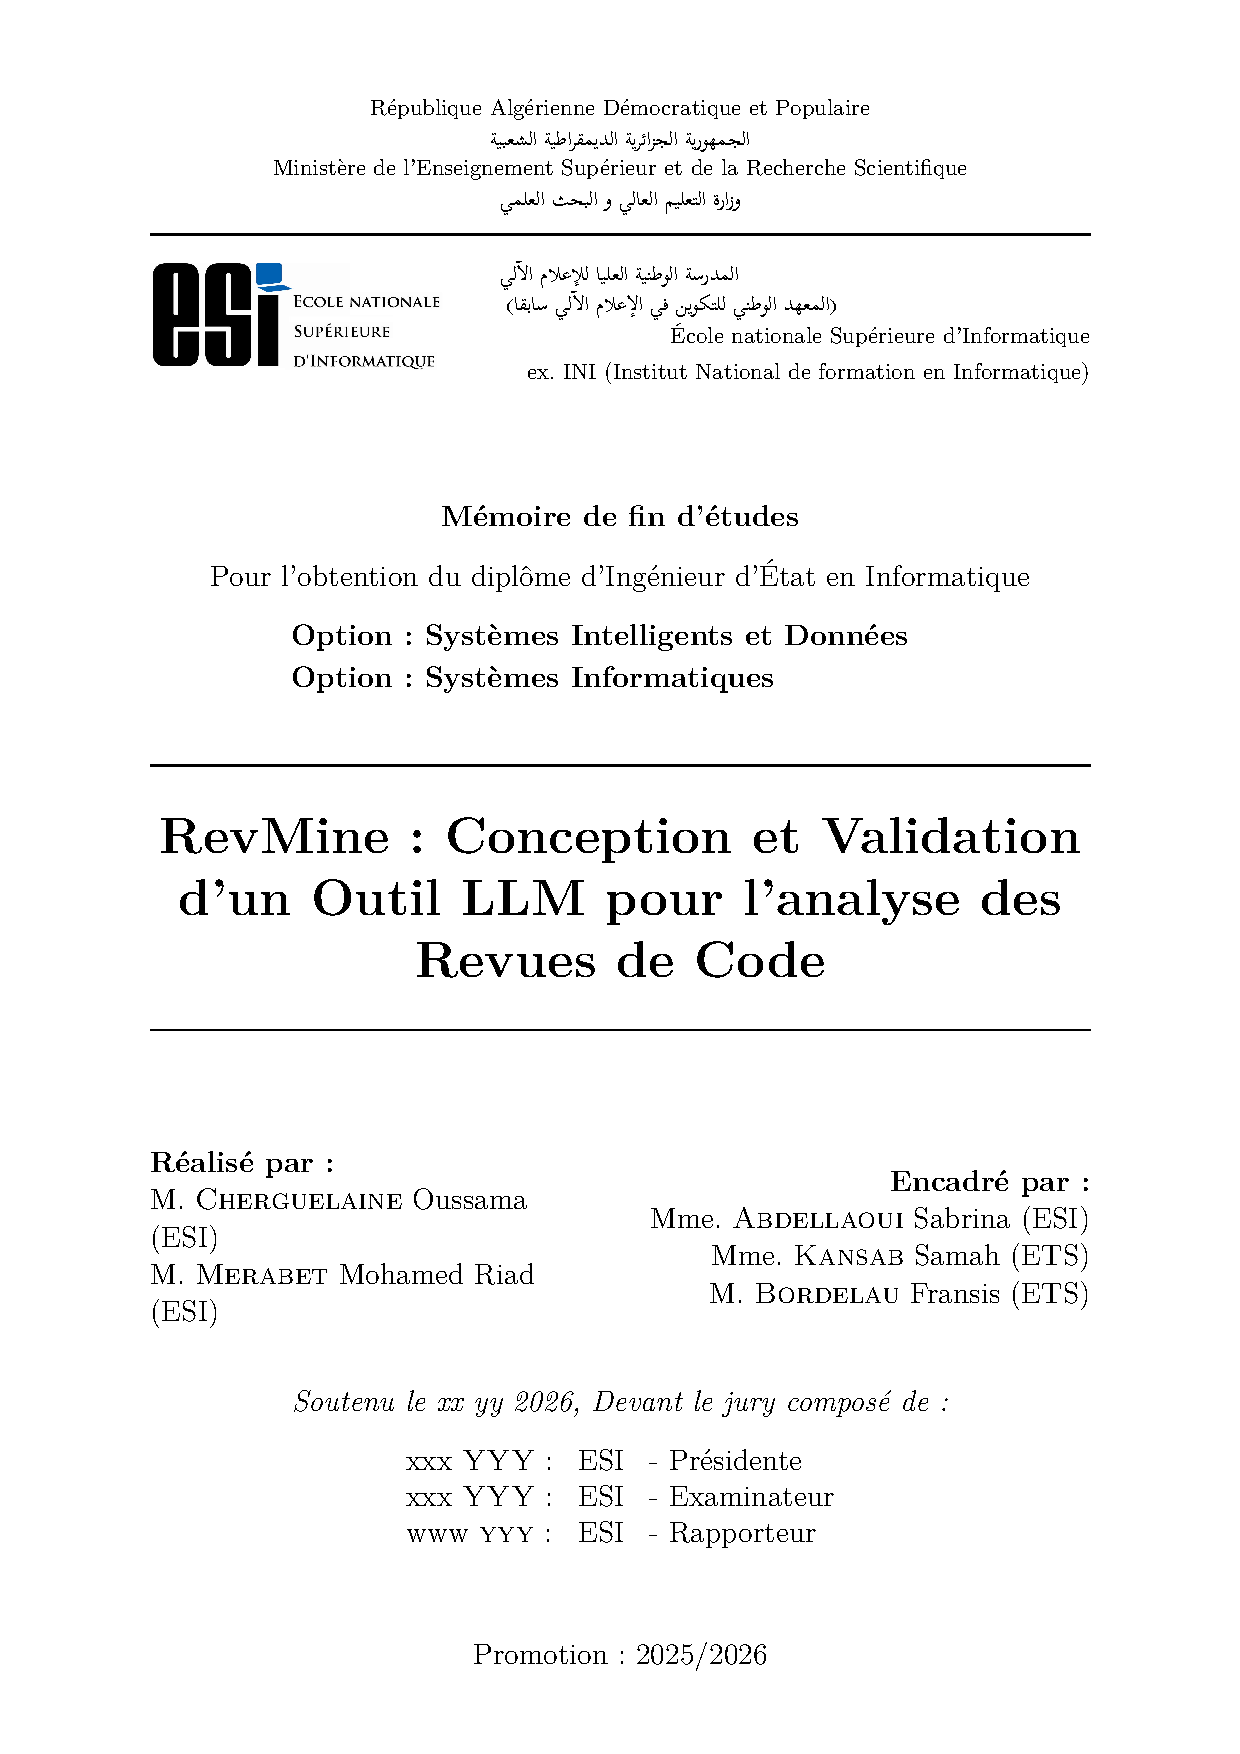
\includepdf[pages=-]{00_Page_De_Garde.pdf}

% =========================
% Pages préliminaires
% =========================
\pagenumbering{Roman}

\mychapter{0}{Dédicaces}

\begin{center}
\textbf{\textit{\large Dédicace de Oussama}}
\end{center}

\begingroup
\itshape

À ma très chère mère, source de tendresse, de patience et de force. Ton amour, tes sacrifices et tes prières ont toujours été la lumière qui m'a guidé dans les moments de doute comme dans les moments de réussite. Cette réalisation porte une part de ton courage et de ta confiance inépuisable.

À mon père, pour son soutien constant, ses conseils justes et les valeurs qu'il m'a transmises. Ton sens de la responsabilité, ton exigence et ta présence discrète m'ont appris à avancer avec sérieux, dignité et persévérance.

À ma sœur Maroua, pour son affection, sa bienveillance et sa présence rassurante. Merci pour tes encouragements, pour tes mots simples qui apaisent, et pour cette complicité qui rend les étapes difficiles plus légères.

À mes deux grandes-mères, dont les prières sincères, les sourires et l'aide précieuse m'ont accompagné tout au long de ce parcours. Votre tendresse et votre bénédiction occupent une place particulière dans cette réussite.

À mon amie Maroua, pour son soutien, son écoute et sa fidélité dans les moments importants. Merci d'avoir été présente avec autant de générosité et d'attention.

À Nibras, pour son aide précieuse et son expertise en design graphique, qui ont contribué à donner une meilleure forme visuelle à ce travail.

À tous mes amis, pour les encouragements, les échanges, les moments partagés et la force morale qu'ils m'ont apportée. À toutes les personnes qui m'ont soutenu de près ou de loin, je dédie ce travail avec gratitude.

\endgroup

\vspace{1.5em}
\begin{flushright}
\textbf{\textit{\large{- Oussama}}}
\end{flushright}

\clearpage

\begin{center}
\textbf{\textit{\large Dédicace de Riad}}
\end{center}

\vspace*{0.72\textheight}

\begin{flushright}
\textbf{\textit{\large{- Riad}}}
\end{flushright}

\clearpage

\mychapter{0}{Remerciements}

Nous remercions avant tout Dieu, qui nous a accordé la force, la patience et la volonté nécessaires pour mener ce projet à son terme.

Nous exprimons notre profonde gratitude à nos encadrants pour leur accompagnement, leur disponibilité et la qualité de leurs orientations. Nous remercions tout particulièrement Mme Sabrina de l'École nationale Supérieure d'Informatique, ainsi que Mme Samah Kansab et M. Francis Bordeleau de l'École de technologie supérieure de Montréal, pour leurs conseils, leurs remarques constructives et la confiance qu'ils nous ont accordée tout au long de ce travail.

Nous remercions également l'équipe de recherche de l'ÉTS pour les échanges enrichissants, les retours scientifiques et l'environnement de travail stimulant qui ont contribué à améliorer la qualité de notre projet.

Nos remerciements s'adressent aussi à l'ensemble des enseignants de l'ESI, qui ont participé à notre formation et nous ont transmis les connaissances, la rigueur et l'esprit d'analyse nécessaires à la réalisation de ce mémoire.

Enfin, nous remercions nos familles, nos amis et toutes les personnes qui nous ont soutenus, encouragés et aidés, de près ou de loin, à avancer jusqu'à cette réussite.

\clearpage

\mychapter{0}{Résumé}

La revue de code est une étape clé du développement logiciel moderne. Elle contribue à détecter les défauts, à améliorer la qualité du code, à renforcer la collaboration et à diffuser les bonnes pratiques. L’analyse des données issues des revues de code, notamment les requêtes de fusion, les commentaires et les commits, permet d’évaluer le processus de revue et d’étudier des aspects tels que la productivité des développeurs, l’adaptation des équipes et la charge de révision.

Ces analyses offrent des leviers concrets pour améliorer les pratiques DevOps, en identifiant les causes des ralentissements, des défauts et des problèmes de qualité de code. En effet, lorsqu’elle est mal maîtrisée, la revue de code peut devenir un goulot d’étranglement dans le pipeline DevOps, en retardant les livraisons, en bloquant l’intégration des changements ou en affectant la prise de décision. Une meilleure compréhension des dynamiques de revue permet d’optimiser les priorités et de fluidifier le cycle de développement.

Cependant, l’exploitation de ces données reste complexe. Elle nécessite la maîtrise des interfaces de programmation des plateformes, de l’authentification, de la pagination, des limitations de requêtes et de l’hétérogénéité des formats. Les données collectées doivent ensuite être nettoyées, filtrées, normalisées et transformées en métriques fiables, ce qui rend le processus long, technique et difficilement reproductible.

Ce mémoire présente RevMine, une plateforme à code source ouvert dédiée à la collecte, au nettoyage, au filtrage, à l’analyse et à la visualisation des données de revue de code issues de GitHub et GitLab. RevMine calcule automatiquement des métriques liées aux délais de traitement, aux changements de code, à l’historique des contributions et à l’engagement des réviseurs, puis génère des visualisations interactives.

La plateforme intègre une assistance par modèles de langage, permettant aux utilisateurs d’exprimer leurs besoins en langage naturel. Ce travail contribue ainsi à rendre l’analyse des données de revue de code plus accessible et reproductible pour les chercheurs en génie logiciel empirique ainsi que pour les praticiens DevOps.

\vspace{1em}
\noindent\rule[2pt]{\textwidth}{0.5pt}

\noindent\textbf{Mots clés :} Revue de code, Mining Software Repositories, DevOps, GitHub/GitLab, LLM

\noindent\rule[2pt]{\textwidth}{0.9pt}

\clearpage

\selectlanguage{english}
\section*{Abstract}

Code review is a key activity in modern software development. It helps detect defects, improve code quality, strengthen collaboration, and promote the sharing of best practices. The analysis of code review data, including pull/merge requests, comments, and commits, makes it possible to evaluate the review process and study important aspects such as developer productivity, team adaptability, and review workload.

Such analyses provide valuable insights for improving DevOps practices by identifying the causes of delays, defects, and code quality issues. When not properly managed, code review may become a bottleneck in the DevOps pipeline, delaying deliveries, blocking the integration of changes, or affecting decision-making. A better understanding of review dynamics can therefore help optimize priorities and improve the overall development cycle.

However, exploiting these data remains challenging. It requires knowledge of platform APIs, authentication mechanisms, pagination, request limits, and heterogeneous data formats. In addition, the collected data must be cleaned, filtered, normalized, and transformed into reliable metrics, which makes the process time-consuming, technical, and difficult to reproduce.

This dissertation presents RevMine, an open-source platform dedicated to the collection, cleaning, filtering, analysis, and visualization of code review data from GitHub and GitLab. RevMine automatically computes metrics related to processing time, code changes, contribution history, and reviewer engagement, then generates interactive visualizations to support analysis.

The platform also integrates language-model assistance, allowing users to express their needs in natural language. This work therefore contributes to making code review data analysis more accessible and reproducible for both empirical software engineering researchers and DevOps practitioners.

\vspace{1em}
\noindent\rule[2pt]{\textwidth}{0.5pt}

\noindent\textbf{Keywords:} Code Review, Mining Software Repositories, DevOps, GitHub/GitLab, LLM

\noindent\rule[2pt]{\textwidth}{0.9pt}

\selectlanguage{french}
\clearpage

\begin{otherlanguage*}{arabic}
\section*{ملخص}

تُعد مراجعة الشيفرة مرحلة أساسية في تطوير البرمجيات الحديثة، إذ تساعد على اكتشاف العيوب، وتحسين جودة الشيفرة، وتعزيز التعاون بين المطورين، ونشر الممارسات الجيدة داخل فرق العمل. ويسمح تحليل البيانات الناتجة عن مراجعات الشيفرة، مثل طلبات الدمج، والتعليقات، والالتزامات البرمجية، بفهم سير عملية المراجعة وقياس جوانب مهمة مثل زمن المعالجة، وعبء المراجعة، ومشاركة المراجعين.

غير أن استغلال هذه البيانات يبقى عملية معقدة، لأنه يتطلب التعامل مع واجهات برمجة التطبيقات الخاصة بمنصات GitHub وGitLab، وآليات المصادقة، وترقيم الصفحات، وحدود الطلبات، واختلاف صيغ البيانات بين المنصات. كما يجب تنظيف البيانات المجمعة، وترشيحها، وتوحيدها، وتحويلها إلى مقاييس قابلة للاستعمال، مما يجعل العملية طويلة وصعبة التكرار.

يقدم هذا العمل منصة RevMine، وهي منصة مفتوحة المصدر مخصصة لجمع بيانات مراجعة الشيفرة من GitHub وGitLab، وتنظيفها، وتحليلها، وعرض نتائجها بصريا. تحسب المنصة مجموعة من المقاييس المتعلقة بزمن المراجعة، وحجم التغييرات، وتاريخ المساهمات، وتفاعل المراجعين، ثم تولد تصورات تفاعلية تساعد الباحثين والممارسين في مجال DevOps على فهم عملية المراجعة وتحسينها.

كما تدمج المنصة مساعدة قائمة على نماذج اللغة الكبيرة، مما يسمح للمستخدم بالتعبير عن احتياجاته باللغة الطبيعية وتحويلها إلى خطة جمع وتحليل منظمة. وبذلك يساهم هذا المشروع في جعل تحليل بيانات مراجعة الشيفرة أكثر سهولة، وقابلية للتكرار، وفائدة للبحث في هندسة البرمجيات التجريبية ولممارسات DevOps.

\vspace{1em}
\noindent\rule[2pt]{\textwidth}{0.5pt}

\noindent\textbf{الكلمات المفتاحية:} مراجعة الشيفرة، تنقيب مستودعات البرمجيات، DevOps، GitHub/GitLab، نماذج اللغة الكبيرة

\noindent\rule[2pt]{\textwidth}{0.9pt}
\end{otherlanguage*}

\selectlanguage{french}
\clearpage

% \mychapter{0}{Glossaire}

Ce glossaire présente les principaux termes et concepts utilisés tout au long de ce mémoire.

\vspace{1em}

\begin{description}
    \item[Revue de code (Code Review)] Processus systématique d'examen du code source par des pairs développeurs dans le but de détecter les défauts, d'améliorer la qualité du code et de partager les connaissances au sein d'une équipe.
    
    \item[Pull Request (PR) / Merge Request (MR)] Mécanisme permettant à un développeur de proposer des modifications de code à un projet. Les autres membres de l'équipe peuvent alors examiner, commenter et approuver ces modifications avant leur intégration.
    
    \item[LLM (Large Language Model)] Modèle de langage de grande taille basé sur l'apprentissage profond, capable de comprendre et de générer du texte en langage naturel. Exemples : GPT, Claude, LLaMA.
    
    \item[DevOps] Approche combinant le développement logiciel (Dev) et les opérations informatiques (Ops) visant à raccourcir le cycle de développement et à fournir des livraisons continues de haute qualité.
    
    \item[API (Application Programming Interface)] Interface de programmation permettant à différentes applications de communiquer entre elles. GitHub et GitLab fournissent des APIs pour accéder aux données des dépôts.
    
    \item[Bottleneck (Goulot d'étranglement)] Point de congestion dans un processus qui ralentit l'ensemble du flux de travail. Dans le contexte DevOps, une revue de code inefficace peut devenir un bottleneck.
    
    \item[GitLab] Plateforme web de gestion de versions basée sur Git, offrant des fonctionnalités de revue de code, d'intégration continue et de déploiement continu.
    
    \item[GitHub] Plateforme d'hébergement de code source utilisant Git, proposant des outils de collaboration, de revue de code et de gestion de projets.
    
    \item[Commit] Enregistrement d'une modification dans l'historique d'un dépôt Git, incluant les changements apportés au code ainsi qu'un message descriptif.
    
    \item[Dataset] Ensemble de données collectées et organisées dans un format structuré, utilisé pour l'analyse et la recherche.
    
    \item[Ingénierie Logicielle Empirique] Approche de recherche en génie logiciel basée sur l'observation, l'expérimentation et l'analyse de données réelles provenant de projets logiciels.
    
    \item[Open Source] Logiciel dont le code source est accessible publiquement, permettant à quiconque de l'examiner, le modifier et le distribuer.
    
    \item[Pipeline DevOps] Ensemble automatisé de processus permettant de passer du code source au déploiement en production, incluant les tests, la revue de code, et l'intégration continue.
    
    \item[Pagination] Technique de division de grandes quantités de données en pages plus petites lors de requêtes API, permettant de gérer efficacement les limitations de transfert de données.
    
    \item[Authentification] Processus de vérification de l'identité d'un utilisateur ou d'une application, souvent nécessaire pour accéder aux APIs des plateformes comme GitHub ou GitLab.
    
    \item[RevMine] Outil développé dans le cadre de ce projet, conçu pour faciliter la collecte et l'analyse des données de revue de code à partir de plateformes comme GitHub et GitLab.
    
\end{description}

\clearpage

\tableofcontents
\clearpage

\listoffigures
\clearpage

\listoftables
\clearpage

\addcontentsline{toc}{chapter}{\listalgorithmname}
\listofalgorithms
\clearpage

\addcontentsline{toc}{chapter}{\listequationsname}
\listofmyequations
\clearpage

% =========================
% Début du mémoire (chiffres arabes)
% =========================
\pagenumbering{arabic}

% =========================
% Introduction générale
% =========================
\let\oldthesection\thesection

\mychapter{}{Introduction générale}
\renewcommand{\thesection}{\arabic{section}}
\section{Contexte}

Dans le développement logiciel moderne, la revue de code est devenue une pratique incontournable pour garantir la qualité et la maintenabilité des applications. Cette pratique consiste à examiner systématiquement le code source écrit par les développeurs avant son intégration dans la base de code principale. Au-delà de la simple détection de bugs, la revue de code favorise le partage de connaissances, l'uniformisation des pratiques de codage et l'apprentissage collectif au sein des équipes.

Avec l'adoption massive des méthodologies Agiles et DevOps, les cycles de développement se sont accélérés, multipliant ainsi le nombre de modifications de code à réviser. Les plateformes de gestion de versions comme GitHub et GitLab sont devenues centrales dans ce processus, offrant des outils intégrés pour faciliter les revues via les requêtes de fusion (Pull Requests (PR) / Merge Requests (MR)). Ces plateformes génèrent d'importantes quantités de données : commentaires, approbations, rejets, temps de révision, historiques de modifications, etc.

L’exploitation de ces données représente une opportunité majeure pour comprendre et optimiser les processus de développement. Dans le domaine de l’ingénierie logicielle empirique, les travaux de Mining Software Repositories montrent l’intérêt croissant de l’analyse des données issues des dépôts logiciels pour extraire des connaissances actionnables sur les projets et leurs processus \cite{vidoni2022systematic}. Dans un contexte DevOps, ces données permettent d’évaluer la performance des équipes, d’identifier les ralentissements dans le cycle de livraison et d’orienter les actions d’amélioration continue \cite{debellis2024dora,kudrjavets2024speed}. Elles sont également utilisées pour étudier la collaboration entre développeurs, la dynamique des revues de code et les risques associés aux changements proposés \cite{bacchelli2013expectations,gocmen2025enhanced}.

Cependant, l’accès à ces données et leur analyse restent problématiques. La collecte nécessite une connaissance approfondie des APIs des plateformes, une gestion complexe de l'authentification, de la pagination et des quotas de requêtes. De plus, les formats de données sont hétérogènes et nécessitent un traitement important avant toute analyse exploitable. Cette complexité technique constitue un frein majeur pour les chercheurs et les équipes souhaitant tirer parti de ces données.

\section{Présentation de l’organisme d’accueil et du cadre de collaboration}
Ce projet de fin d’études a été réalisé au sein de l’École nationale Supérieure d’Informatique d’Alger (ESI), en collaboration avec l’École de technologie supérieure de Montréal (ÉTS). Ce cadre de collaboration a permis d’associer un environnement de formation en ingénierie informatique à une expertise de recherche appliquée en génie logiciel.

L’École nationale Supérieure d’Informatique d’Alger est un établissement algérien spécialisé dans la formation supérieure en informatique. Créée en 1969 sous le nom de Centre d’Études et de Recherche en Informatique (CERI), elle est devenue l’Institut National de Formation en Informatique (INI) avant d’être transformée en École nationale supérieure en 2008. L’ESI assure notamment une formation d’ingénieur d’État en informatique sur cinq années, articulée autour d’un cycle préparatoire et d’un second cycle de spécialisation \cite{esiPresentation}.

L’École de technologie supérieure de Montréal est une université québécoise spécialisée en génie appliqué. Sa mission repose sur l’enseignement universitaire, la recherche appliquée et le transfert technologique, en lien étroit avec l’industrie. L’ÉTS occupe une place importante dans la formation en ingénierie au Québec, puisqu’elle forme une part significative des ingénieurs québécois et s’inscrit dans une dynamique d’innovation technologique \cite{etsAccueil}.

Dans ce contexte, le projet RevMine s’inscrit dans une collaboration académique entre l’ESI et l’ÉTS. La réalisation du projet a été encadrée côté ESI par notre encadrante académique, tandis que l’accompagnement scientifique côté ÉTS a été assuré par les promotrices associées au projet. Cette organisation a permis de bénéficier à la fois d’un suivi académique local et d’une expertise de recherche spécialisée dans l’analyse des processus logiciels et des données de revue de code.

La figure suivante illustre l’organisation de l’encadrement du projet RevMine. Elle met en évidence les étudiants porteurs du projet, l’encadrement assuré par l’ESI Alger ainsi que la collaboration scientifique avec l’ÉTS Montréal.


\begin{figure}[H]
\centering
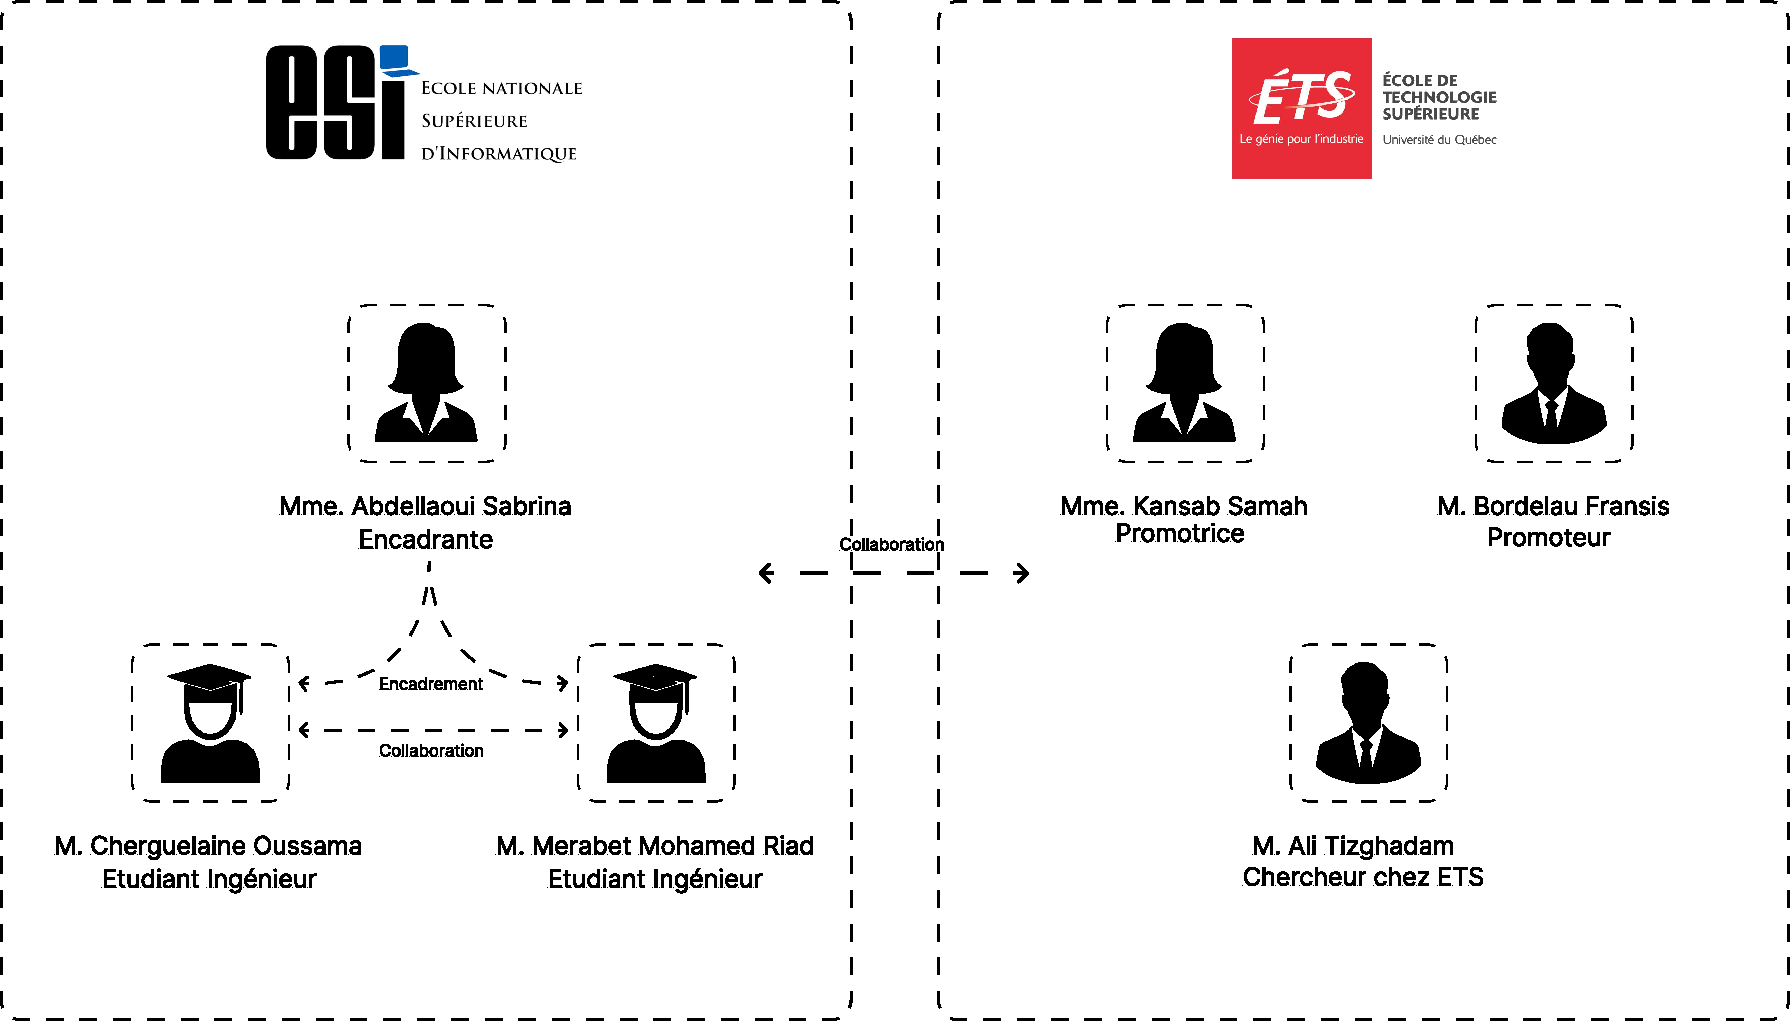
\includegraphics[width=0.9\textwidth]{figures/organisme_d_acceuil.pdf}
\caption{Organisation du projet RevMine}
\label{fig:encadrement-revmine}
\end{figure}


\section{Problématique}

Malgré l'importance croissante de la revue de code dans les pratiques DevOps et l'abondance de données générées par les plateformes comme GitHub et GitLab, plusieurs obstacles limitent leur exploitation efficace :

\begin{itemize}
     \item \textbf{Complexité de préparation de la collecte :}
    L’exploitation des données de revue de code ne se limite pas à l’appel des APIs. Elle nécessite un effort manuel important pour comprendre la structure des plateformes, sélectionner les bons points d’accès, gérer l’authentification, la pagination, les erreurs, les filtres de collecte et la normalisation des données. Cette phase de préparation impose souvent l’écriture de scripts spécifiques et rend le processus difficilement accessible aux utilisateurs non experts, en particulier lorsque l’objectif est de produire une collecte fiable et reproductible \cite{gousios2012ghtorrent,duenas2018perceval,vidoni2022systematic}.
    
    \item \textbf{Hétérogénéité des formats :} Les données provenant de différentes sources (GitHub, GitLab) présentent des structures et des formats variés, nécessitant des transformations et normalisations spécifiques.
    
    \item \textbf{Absence d'outils intégrés :} Il n'existe pas de solution unifiée permettant à la fois la collecte, le nettoyage, l'analyse et la visualisation des données de revue de code de manière accessible aux non-experts.
    
    \item \textbf{Barrière d'accessibilité :} Les chercheurs et praticiens qui ne possèdent pas de compétences avancées en programmation ou en manipulation d'APIs sont souvent exclus de ce type d'analyses.
    
    \item \textbf{Manque d'interactivité :} Les outils existants proposent généralement des analyses prédéfinies, sans permettre aux utilisateurs de formuler leurs propres questions ou d'explorer librement les données selon leurs besoins spécifiques.
\end{itemize}

Face à ces constats, la question centrale de ce projet est : \textbf{Comment faciliter l'accès, la collecte et l'analyse des données de revue de code pour les rendre exploitables par un large public, tout en offrant une interface intuitive et interactive ?}

\section{Objectifs}

Pour répondre à cette problématique, ce projet de fin d'études vise à développer \textbf{RevMine}, un outil interactif et accessible pour la collecte et l'analyse des données de revue de code. Les objectifs spécifiques sont les suivants :
\FloatBarrier
\begin{table}[h]
\centering
\caption{Objectifs du projet RevMine}
\label{tab:objectifs_smart}
\begin{tabular}{|c|p{0.8\textwidth}|}
\hline
\textbf{ID} & \textbf{Objectif} \\
\hline
\textbf{O1} & Réduire le temps de collecte de données de revue de code depuis GitHub et GitLab de 70\% en gérant l’authentification, la pagination et la normalisation. \\
\hline
\textbf{O2} & Développer une interface no-code accessible aux non-experts permettant la configuration complète sans programmation. \\
\hline
\textbf{O3} & Centraliser les phases de collecte, nettoyage, analyse et visualisation dans une plateforme unique, éliminant le besoin de recourir à 3-4 outils séparés. \\
\hline
\textbf{O4} & Intégrer un module LLM réduisant de 80\% le temps de personnalisation via requêtes en langage naturel et génération automatique d'analyses. \\
\hline
\textbf{O5} & Valider RevMine sur 3+ projets open source de tailles variées avec collecte réussie de plus de 90\% des données disponibles. \\
\hline
\textbf{O6} & Produire une documentation complète (installation, tutoriels, architecture) et un package de réplication open source. \\
\hline
\end{tabular}
\end{table}
\FloatBarrier
% \subsection{Objectif 1 : Collecte automatisée des données}

% Développer un module robuste capable de collecter automatiquement les données de revue de code à partir des APIs de GitHub et GitLab, en gérant :
% \begin{itemize}
%     \item L'authentification sécurisée
%     \item La pagination pour récupérer de grands volumes de données
%     \item Les quotas et limitations d'API
%     \item La gestion des erreurs et la reprise en cas d'échec
%     \item La normalisation des formats de données
% \end{itemize}

% \subsection{Objectif 2 : Interface utilisateur intuitive}

% Concevoir une interface graphique conviviale permettant :
% \begin{itemize}
%     \item La configuration facile des sources de données (dépôts, tokens d'accès)
%     \item Le suivi en temps réel de la progression de la collecte
%     \item L'exploration visuelle des données collectées
%     \item La sélection guidée des analyses à effectuer
% \end{itemize}

% \subsection{Objectif 3 : Intégration d'un module LLM pour les requêtes en langage naturel}

% Intégrer un modèle de langage (LLM) permettant aux utilisateurs de :
% \begin{itemize}
%     \item Formuler leurs questions d'analyse en langage naturel
%     \item Obtenir des réponses contextualisées basées sur les données collectées
%     \item Générer automatiquement des scripts d'analyse ou des visualisations
%     \item Bénéficier de suggestions d'analyses pertinentes
% \end{itemize}

% \subsection{Objectif 4 : Validation sur des projets open source}

% Valider l'outil sur plusieurs projets open source représentatifs pour :
% \begin{itemize}
%     \item Démontrer sa capacité à gérer différents types et tailles de projets
%     \item Collecter des datasets de référence utilisables par la communauté de recherche
%     \item Identifier et corriger les limitations de l'outil
%     \item Produire des analyses concrètes démontrant l'utilité de RevMine
% \end{itemize}

% \subsection{Objectif 5 : Documentation et reproductibilité}

% Fournir une documentation complète comprenant :
% \begin{itemize}
%     \item Un guide d'installation et de configuration
%     \item Des tutoriels d'utilisation avec exemples
%     \item Une documentation technique de l'architecture
%     \item Des exemples d'analyses reproductibles
% \end{itemize}

\section{Structure du mémoire}

Ce mémoire est structuré en deux grandes parties complémentaires, précédées d’une introduction générale et suivies d’une conclusion générale.

\textbf{Première partie : Étude bibliographique}

La première partie de ce mémoire présente les fondements théoriques et le contexte scientifique du projet RevMine. Elle vise à introduire les concepts essentiels liés à la revue de code, aux pratiques DevOps, à l’analyse des données logicielles, ainsi qu’à l’utilisation des modèles de langage (LLMs) dans l’ingénierie logicielle.

Le premier chapitre propose un état de l’art sur la revue de code et son rôle dans les pipelines DevOps modernes. Il aborde également les différentes approches d’analyse des données de développement logiciel ainsi que l’intégration des modèles de langage dans ces processus.

Le second chapitre est consacré à l’étude de l’existant. Il présente une analyse comparative des outils actuels de collecte et d’analyse des données issues des plateformes telles que GitHub et GitLab. Cette étude met en évidence les limites des solutions existantes et justifie la nécessité d’un outil comme RevMine.

\textbf{Deuxième partie : Contribution}

La deuxième partie de ce mémoire est dédiée à la contribution principale de ce projet, à savoir la conception, le développement et la validation de la plateforme RevMine.

Le premier chapitre de cette partie présente l’analyse des besoins, en identifiant les différents acteurs du système ainsi que les exigences fonctionnelles et non fonctionnelles auxquelles la plateforme doit répondre.

Le second chapitre décrit la conception de la solution proposée. Il détaille l’architecture générale du système, les différents modules, ainsi que les choix techniques et architecturaux adoptés.

Le troisième chapitre présente les métriques et les visualisations supportées par RevMine, en mettant en évidence leur intérêt pour l’analyse des processus de revue de code.

Le quatrième chapitre expose la réalisation de la plateforme. Il décrit les technologies utilisées, l’architecture microservices mise en place, ainsi que les différents composants développés, tant au niveau du backend que du frontend.

Enfin, un dernier chapitre est consacré à la validation et à l’évaluation de la solution proposée. Il présente les tests réalisés, les résultats obtenus ainsi que les limites du système.

Le mémoire se termine par une conclusion générale qui synthétise les contributions réalisées et propose des perspectives d’amélioration.
\let\thesection\oldthesection
% =========================================================
% PARTIE I : Fondements et analyse de l'existant
% =========================================================
\part{État de l'art et étude des solutions commerciales existantes}

\chapter{État de l'art}

\section{Notions de base}

\subsection{Processus DevOps}

Le DevOps désigne une approche organisationnelle et technique visant à rapprocher le développement logiciel et les opérations informatiques afin d’améliorer la rapidité, la fiabilité et la continuité de la livraison logicielle. Il repose notamment sur l’automatisation, l’intégration continue, la livraison continue, la collaboration entre équipes et l’amélioration continue des processus \cite{bass2015devops,leite2020devops}.

Dans ce mémoire, le DevOps constitue le cadre général dans lequel s’inscrit la revue de code. En effet, les modifications de code doivent être conçues, implémentées, vérifiées, révisées puis intégrées avant d’être livrées. La revue de code intervient donc comme une étape de contrôle et de collaboration au sein du cycle de développement logiciel.



\subsection{Pipeline DevOps}

Un pipeline DevOps désigne un enchaînement automatisé et structuré d’étapes permettant de faire évoluer une modification logicielle depuis le code source jusqu’à sa livraison ou son déploiement. Il inclut généralement des phases telles que la compilation, les tests automatisés, l’analyse qualité, la validation, le déploiement et la surveillance. Selon l’organisation du projet, la revue de code peut également constituer une étape préalable à l’intégration des changements dans la branche principale \cite{humble2010continuous,shahin2017continuous}.

L’objectif d’un tel pipeline est de rendre la livraison logicielle plus rapide, fiable et répétable. Toute interruption ou attente prolongée dans l’une de ses étapes peut ralentir le cycle global de livraison.



\subsection{Revue de code}

La revue de code est une activité consistant à examiner le code source produit par un développeur avant son intégration dans la base de code principale. Les inspections formelles de code ont été popularisées par les travaux de Fagan, qui ont montré leur intérêt pour la détection précoce des défauts et la réduction des coûts de correction \cite{fagan1976design}.

Dans les environnements modernes, la revue de code est généralement réalisée de manière outillée et asynchrone à travers des plateformes collaboratives. Elle ne se limite pas à la détection d’erreurs : elle contribue également à améliorer la qualité du code, à assurer le respect des conventions, à favoriser le partage de connaissances et à renforcer la collaboration entre développeurs \cite{bacchelli2013expectations,mcintosh2014impact}.



\subsection{Plateformes de développement collaboratif}

Les plateformes de développement collaboratif, telles que GitHub et GitLab, sont des environnements permettant d’héberger des dépôts logiciels, de gérer l’historique du code source et de coordonner le travail entre développeurs. Elles offrent des fonctionnalités telles que la gestion des branches, le suivi des issues, les requêtes de fusion, les commentaires de revue, les permissions d’accès et, dans certains cas, l’intégration et le déploiement continus.

Ces plateformes jouent un rôle central dans le développement logiciel distribué, car elles fournissent à la fois l’infrastructure technique de gestion du code et les mécanismes de collaboration nécessaires à la revue et à l’intégration des changements \cite{kalliamvakou2014promises,github_about_pr,gitlab_merge_requests}.



\subsection{Logiciel à code source ouvert}
Un logiciel à code source ouvert, ou open source, est un logiciel dont les conditions de distribution permettent l’accès au code source, sa redistribution et la création de versions modifiées. Selon l’Open Source Initiative, l’accès au code source ne suffit pas à lui seul : la licence doit également autoriser la redistribution et les travaux dérivés selon des conditions compatibles avec la définition de l’open source. Dans ce mémoire, cette notion est importante à deux niveaux : d’une part, RevMine est développé comme une plateforme à code source ouvert ; d’autre part, les projets open source constituent des sujets d’étude privilégiés pour la collecte et la validation expérimentale \cite{osi_osd}.


\subsection{Requête de fusion (Pull Request / Merge Request)}

Une requête de fusion (Pull Request sur GitHub ou Merge Request sur GitLab) est un mécanisme permettant à un développeur de proposer l’intégration de ses modifications dans une branche cible.

Comme le décrivent \cite{gousios2014exploratory}, elle constitue le support principal du modèle de développement basé sur les contributions (pull-based development), en centralisant les modifications de code, l’historique des commits, ainsi que les discussions et commentaires associés. Elle est ainsi au cœur du processus de revue de code moderne.

\subsection{Cycle de vie d’une requête de fusion}
\begin{figure}[H]
\centering
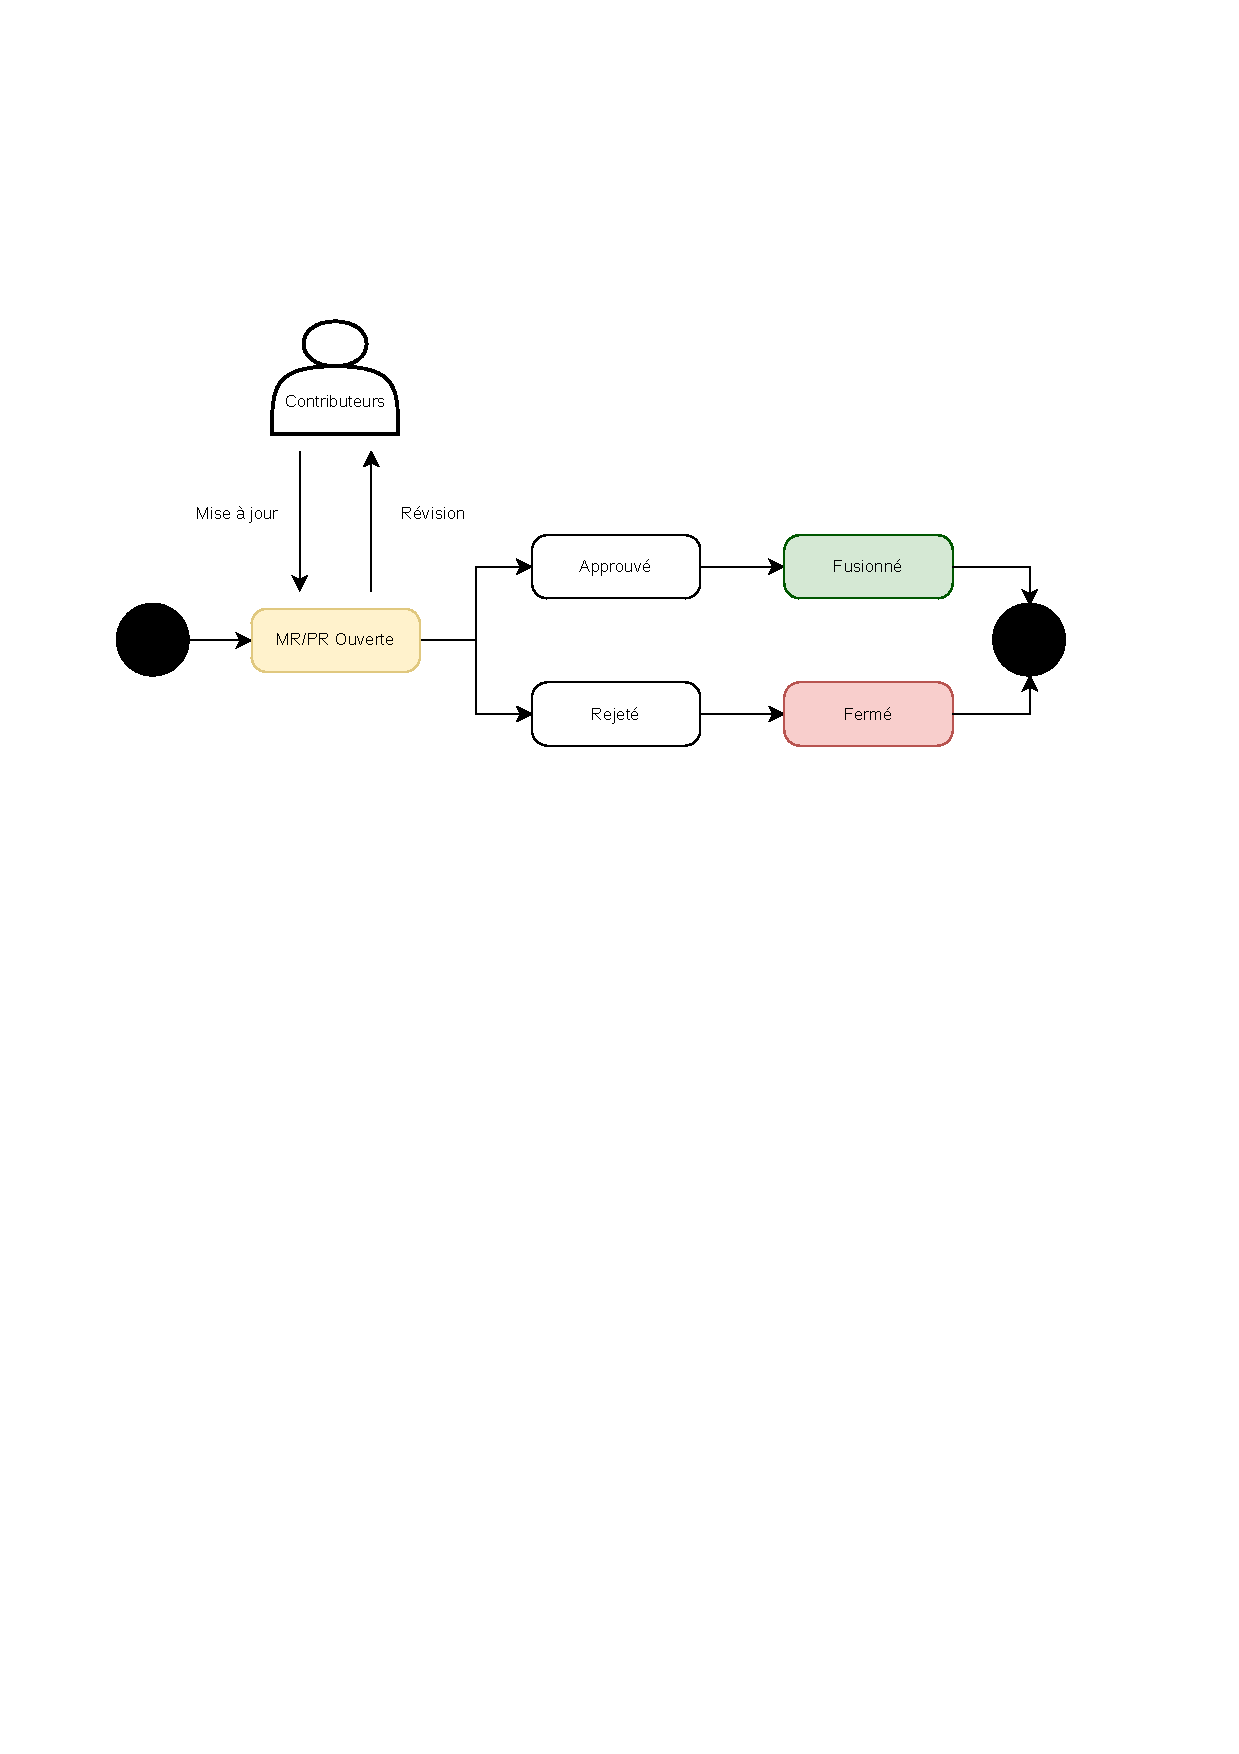
\includegraphics[width=0.8\textwidth, height=0.6\textheight, keepaspectratio]{figures/diag-mrlc (1).pdf}
\caption{\label{fig:lc}Cycle de vie d’une requête de fusion}
\end{figure}
Dans ce mémoire, nous considérons le cycle de vie d’une requête de fusion tel qu’illustré à la figure \ref{fig:lc}. Une requête de fusion peut passer par plusieurs états :

\begin{itemize}
\item \textbf{Ouverte :} Il s’agit de l’état initial au moment de la création d’une requête de fusion. Cet état indique que la requête est disponible pour révision et discussion.
\item \textbf{Fermée :} La requête a été clôturée sans qu’une fusion ait été effectuée. Cela peut se produire lorsque les modifications proposées ne sont plus nécessaires, jugées inappropriées ou lorsque certains problèmes ne peuvent pas être résolus.

\item \textbf{Fusionnée :} Les changements proposés ont été validés et intégrés dans la branche cible. Le code est désormais inclus dans la base de code principale.

\item \textbf{Autres états :} Dans certains cas, les développeurs marquent leurs requêtes comme « Work In Progress (WIP) » ou « brouillon » afin de partager l’avancement de leur travail sans solliciter immédiatement une révision.
\end{itemize}

\subsection{Commit}

Un commit est une unité d’enregistrement dans l’historique d’un dépôt Git. Il représente un ensemble cohérent de modifications appliquées à un ou plusieurs fichiers, accompagné d’un message décrivant les changements réalisés. Chaque commit possède un identifiant unique, généralement appelé hash ou SHA, qui permet de le retrouver dans l’historique du projet \cite{github_about_commits}.

Dans le contexte des revues de code, les commits associés à une requête de fusion permettent d’analyser l’évolution des changements proposés, le volume de code modifié et le rythme de contribution.



% \begin{figure}
% \centering
% \includegraphics[width=0.8\textwidth, height=0.6\textheight, keepaspectratio]{figures/diag-mrlc.pdf}
% \caption{\label{fig:lc}Cycle de vie d’une requête de fusion}
% \end{figure}

\subsection{Acteurs de la revue de code}

Comme le montre la figure \ref{fig:mc}, plusieurs acteurs interviennent dans le processus de revue d’une requête de fusion afin d’en assurer l’efficacité et la qualité :

\begin{itemize}
\item \textbf{Auteur :} Le développeur qui a soumis les modifications et créé la requête de fusion. Il est chargé d’envoyer les demandes de révision et de répondre aux commentaires formulés par les réviseurs.

\item \textbf{Contributeurs (Committers) :} Ce groupe regroupe les membres de l’équipe travaillant sur les changements proposés, y compris l’auteur. Ils sont responsables des mises à jour successives du code.

\item \textbf{Réviseurs :} Les personnes en charge d’examiner le nouveau code afin d’en évaluer la qualité, la cohérence et la conformité. Ils échangent avec les contributeurs pour proposer des corrections ou des améliorations.

\item \textbf{Commentateurs :} Tous les participants (auteurs, contributeurs, réviseurs ou autres intervenants) qui laissent des commentaires pour discuter des modifications apportées. GitLab permet également à des bots d’ajouter des commentaires automatiques pour fournir des informations standardisées.

\item \textbf{Intégrateur :} L’individu chargé de décider si la requête doit être fusionnée, rejetée ou encore modifiée. Ce rôle peut être tenu par l’auteur ou un autre membre de l’équipe de contributeurs.

\end{itemize}

\begin{figure}[H]
\centering
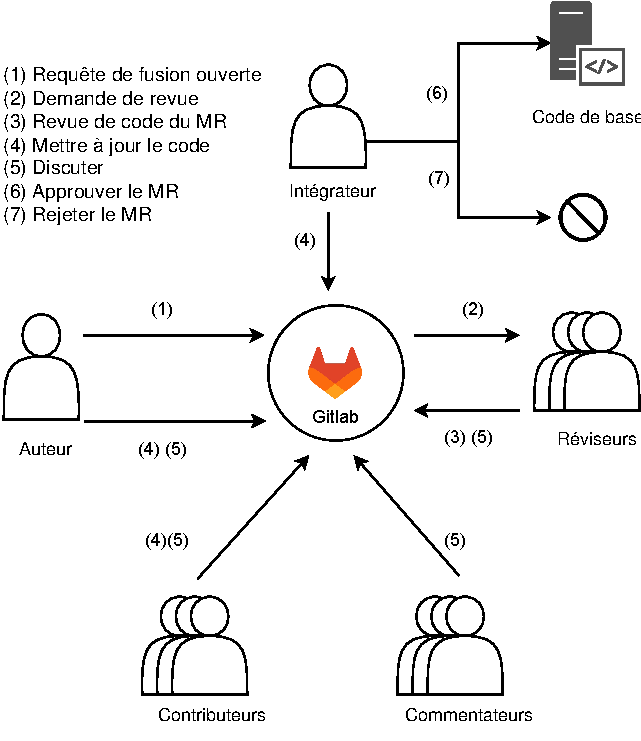
\includegraphics[width=0.8\textwidth, height=0.4\textheight]{figures/diag-Mrm (1).pdf}
\caption{\label{fig:mc}Mécanisme d’interaction autour d’une requête de fusion}
\end{figure}



\subsection{Goulot d’étranglement en revue de code}

Un goulot d’étranglement désigne un point de ralentissement qui limite la progression globale d’un processus. Dans un contexte DevOps, la revue de code peut devenir un goulot d’étranglement lorsque les requêtes de fusion restent en attente trop longtemps, lorsque les réviseurs ne sont pas disponibles ou lorsque les échanges nécessaires à la validation prennent un temps excessif.

Ces ralentissements peuvent retarder l’intégration des changements et affecter la vitesse de livraison. Des travaux récents montrent que le temps de réaction et le temps jusqu’à la fusion sont des préoccupations importantes pour les praticiens, car ils influencent directement la vélocité du développement \cite{kudrjavets2024speed}. D’autres travaux ont également montré que la couverture et la participation dans la revue de code sont liées à la qualité logicielle \cite{mcintosh2014impact}.





\subsection{Métriques en ingénierie logicielle}

Les métriques logicielles sont des indicateurs quantitatifs utilisés pour évaluer les processus et les produits logiciels.  \cite{fenton2014software} soulignent qu’elles doivent être valides, fiables et exploitables.

Avec l’évolution du génie logiciel, l’utilisation de métriques est devenue essentielle pour améliorer les pratiques DevOps. Les métriques DORA (DevOps Research and Assessment) ont été largement adoptées comme référence pour évaluer la performance des équipes.

Cependant, des métriques plus spécifiques sont aujourd’hui utilisées pour analyser des aspects précis, notamment la revue de code. Dans ce contexte, on s’intéresse à des indicateurs tels que le temps de revue (lead time), l’engagement des réviseurs ou encore le volume de modifications (code churn).

\subsection{Ingénierie logicielle empirique et Mining Software Repositories}

L’ingénierie logicielle empirique est une approche de recherche qui étudie les produits, les processus et les pratiques du développement logiciel à partir d’observations, de mesures et de données issues de projets réels. Elle permet de formuler, vérifier ou nuancer des conclusions sur le fonctionnement effectif des équipes et des systèmes logiciels.

Dans ce cadre, le Mining Software Repositories consiste à exploiter les données provenant de dépôts logiciels et de plateformes de développement afin d’extraire des connaissances sur l’évolution du code, la collaboration, la qualité logicielle et les processus de développement. Les travaux de ce domaine soulignent l’importance de protocoles de collecte et d’analyse systématiques afin de garantir la validité et la reproductibilité des résultats \cite{hassan2008road,vidoni2022systematic}.

% \subsection{Jeu de données}

% Un jeu de données, ou dataset, désigne un ensemble organisé de données collectées, structurées et préparées en vue d’être analysées, partagées ou réutilisées. Dans ce mémoire, un jeu de données de revue de code regroupe des informations extraites depuis GitHub ou GitLab, telles que les requêtes de fusion, les commits, les commentaires, les dates de création, de fermeture ou de fusion, les auteurs, les réviseurs et les fichiers modifiés.

% La qualité d’un jeu de données dépend de plusieurs facteurs, notamment la complétude des informations collectées, la cohérence des formats, la traçabilité de la collecte et la documentation des métadonnées associées \cite{datacite_metadata_2024}.



Dans ce mémoire, cette notion est importante à deux niveaux. D’une part, RevMine est développé comme une plateforme à code source ouvert. D’autre part, les projets open source constituent des sujets d’étude privilégiés pour la collecte, l’analyse et la validation expérimentale des données de revue de code.

\subsection{Intelligence artificielle générative}

L’intelligence artificielle générative désigne une catégorie de systèmes capables de produire du contenu, tel que du texte, du code, des images ou des structures de données, à partir de modèles appris sur de grands volumes de données. Cette famille de systèmes s’appuie notamment sur des modèles de fondation capables d’être adaptés à plusieurs tâches en aval \cite{bommasani2021foundation}.

Dans le domaine du génie logiciel, l’intelligence artificielle générative est de plus en plus utilisée pour assister certaines activités telles que la génération de code, la documentation, l’aide à la compréhension de programmes, l’analyse de requêtes utilisateur et l’automatisation partielle de tâches de développement \cite{hou2024llmse}.

\subsection{Modèles de langage}

Les grands modèles de langage, ou Large Language Models (LLMs), sont des modèles d’intelligence artificielle entraînés sur de très grands corpus textuels et capables de traiter, générer et transformer du langage naturel. Certains modèles sont également entraînés ou adaptés sur du code source, ce qui leur permet d’être utilisés dans des tâches de génie logiciel \cite{brown2020language,hou2024llmse}.

Dans le contexte de RevMine, les modèles de langage ne remplacent pas les services de collecte ou d’analyse. Ils servent plutôt de couche d’assistance permettant d’interpréter des besoins exprimés en langage naturel et de les transformer en configurations structurées exploitables par la plateforme.

\subsection{Analyse des données de revue de code}

L’analyse des données de revue de code consiste à exploiter les informations produites par les plateformes collaboratives afin de comprendre, mesurer et améliorer les pratiques de revue. Ces informations peuvent inclure les requêtes de fusion, les commits, les commentaires, les approbations, les dates, les auteurs, les réviseurs, les fichiers modifiés et les métadonnées associées.

Cette analyse permet d’étudier des aspects tels que les délais de revue, la charge des réviseurs, l’engagement des participants, le volume de modifications, les zones fréquemment modifiées et les points de ralentissement du processus. Elle s’inscrit ainsi dans une démarche d’ingénierie logicielle empirique et de Mining Software Repositories, où les décisions d’amélioration sont fondées sur des données observables plutôt que sur des impressions subjectives \cite{bacchelli2013expectations,gousios2014exploratory,vidoni2022systematic}.



\section{Étude de literature sur la revue de code}

La revue de code représente une composante essentielle du processus d’amélioration logicielle. De nombreuses recherches ont mis en évidence son rôle déterminant dans la garantie de la qualité du code et la fiabilité des produits logiciels \parencite{tufano2021towards, oh2005reflective}. Elle contribue non seulement à la détection précoce des anomalies, mais aussi à l’amélioration continue des pratiques de développement \parencite{mcintosh2014impact, bavota2015four}.

Plusieurs travaux se sont attachés à identifier les facteurs qui influencent le déroulement et l’efficacité des revues, notamment ceux liés à la qualité du code et aux dynamiques de collaboration entre développeurs \parencite{kononenko2016code, dougan2022towards}.

Toutefois, la dépendance à l’intervention humaine rend le processus sujet à divers aléas : comportements inattendus \parencite{fuggetta2000software}, retards parfois significatifs — pouvant atteindre plusieurs heures \parencite{bosu2013impact} — et variations dans la qualité des révisions \parencite{dougan2022towards}.
Face à ces limites, la communauté scientifique a proposé diverses approches visant à automatiser, rationaliser et optimiser la revue de code afin d’en renforcer la rigueur et l’efficacité.

\subsection{Automatisation de la revue de code}
Pour automatiser le processus de revue de code, \textcite{tufano2021towards} se concentre sur l’amélioration simultanée des rôles du contributeur et du réviseur. Leur approche repose sur deux architectures d’apprentissage profond distinctes, entraînées à partir de scénarios réels de revues de code. Le modèle proposé suggère des modifications à l’auteur avant la soumission officielle, et propose également aux réviseurs des commentaires inspirés de situations similaires déjà rencontrées. Cette méthode a permis d’obtenir 16 \% de suggestions pertinentes du côté des contributeurs et une amélioration de 31 \% du côté des réviseurs.

De leur côté, \textcite{gupta2017deepfix} ont introduit un modèle séquence-à-séquence à plusieurs couches capable d’identifier et de corriger de manière itérative les erreurs présentes dans des programmes écrits en C. Leur approche a réussi à automatiser la correction de 27 \% des échantillons de test. De façon similaire, \textcite{chen2019sequencer} ont développé un modèle destiné à corriger automatiquement les bogues à une seule ligne dans le code Java ; leur meilleure configuration a atteint une précision de 20 \% sur les exemples testés. D’autres travaux se sont intéressés à la complétion de code afin de générer du code correct et prévenir l’introduction d’erreurs \cite{sadovykh2021veridevops, alon2020structural}.

Dans un contexte industriel, l'automatisation de la revue de code demeure un défi complexe en raison de la diversité des environnements de développement, de la fréquence élevée des demandes de revue, de la taille considérable des projets logiciels et de la variabilité des processus entre équipes. Plusieurs études ont proposé des solutions adaptées à ces contraintes. Par exemple, \textcite{kim2022understanding} ont conçu un bot de revue de code pour Samsung Electronics, capable de mesurer la taille des changements soumis, de détecter les fautes de frappe, les défauts potentiels et les violations de style. Les ingénieurs de l’entreprise ont exprimé leur satisfaction face à cet outil, qui leur permet d’accélérer significativement les révisions.

De même, Google a mis au point un système d’analyse et de revue de code intégré à son flux de développement \cite{sadowski2015tricorder, potvin2016google}, tandis que Microsoft a adopté divers outils d’assurance qualité effectuant des analyses automatisées du code \cite{bird2015lessons}. Ces systèmes, bien qu’efficaces, ne suppriment toutefois pas totalement la nécessité d’une intervention humaine dans le processus de revue.

\subsection{Explication du processus de revue de code à l’aide de modèles d’apprentissage automatique}

Les travaux portant sur l’automatisation de la revue de code montrent qu’une automatisation complète du processus reste impossible et nécessitera toujours une intervention humaine. Face à cette limite, plusieurs recherches se sont orientées vers l’utilisation de l’apprentissage automatique afin de mieux comprendre l’influence de divers indicateurs associés aux revues, dans le but d’en améliorer l’efficacité et la rapidité.

Par exemple, \textcite{chouchen2023learning} ont conçu un modèle d’apprentissage automatique capable de prédire le temps nécessaire à la finalisation d’une revue de code, tout en identifiant les facteurs qui influencent cette durée. \textcite{hasan2023understanding} ont montré qu’un délai de première réponse plus court — qu’elle provienne d’un bot ou d’un humain — est généralement associé à une durée de revue plus brève. Toutefois, cette corrélation ne se vérifie pas toujours dans les cas où les bots initient la première interaction, en raison d’une moindre implication des développeurs.

Selon \textcite{bosu2014impact}, les développeurs expérimentés reçoivent un retour initial plus rapide, ce qui se traduit par une réduction du temps global de revue. \textcite{jiang2013will} ont quant à eux démontré que le nombre de réviseurs influe sur la durée du processus. De plus, \textcite{thongtanunam2017review} se sont intéressés aux caractéristiques des correctifs de code qui attirent un plus grand nombre de réviseurs.
D’autres études, telles que celles de \textcite{li2020redundancy} et \textcite{khatoonabadi2023wasted}, se sont penchées sur les demandes de fusion dupliquées ou abandonnées, qui mobilisent inutilement le temps et les efforts des développeurs. Enfin, \textcite{fan2018early} et \textcite{islam2022early} ont proposé des approches permettant de prédire, dès les premières étapes, si les modifications proposées seront intégrées dans la base de code principale.

Dans le contexte industriel, plusieurs études ont également tenté d’expliquer et d’optimiser le processus de revue de code. Chez Microsoft, par exemple, \textcite{maddila2023nudge} ont proposé un modèle capable de prédire la durée des revues, de détecter les activités et d’identifier les acteurs responsables des blocages dans les demandes de fusion. \textcite{hasan2021using} ont présenté une approche globale visant à évaluer et prédire la qualité des revues tout en abordant les défis rencontrés par les réviseurs.
De leur côté, \textcite{wang2019leveraging, wang2021large} ont formulé le problème de l’estimation de l’effort de revue comme une tâche de classification binaire, définissant les revues exigeant un effort important comme celles ayant nécessité plus de deux itérations de correction chez Microsoft. Enfin, \textcite{baysal2016investigating}, dans une étude empirique sur les projets Webkit et Google Blink, ont montré que la durée des revues dépend à la fois de facteurs techniques (liés au code) et non techniques (liés aux interactions humaines).

\subsection{L'intelligence artificielle générative (GenAI) et les grands modèles de langage (LLMs) pour la revue de code}

Les récentes avancées en intelligence artificielle générative (GenAI) et en grands modèles de langage (LLMs) ont considérablement transformé les tâches liées à la revue de code, notamment grâce à l’apprentissage par peu d’exemples (few-shot learning) et aux approches hybrides. \textcite{pornprasit2024fine} ont comparé le fine-tuning et le few-shot prompting de GPT-3.5 et Magicoder, montrant que les méthodes par peu d’exemples améliorent les prédictions préliminaires lorsque les données annotées sont limitées.
De leur côté, \textcite{haider2024prompting} ont démontré que l’enrichissement des invites par des métadonnées sémantiques du code — telles que les graphes d’appels de fonctions — permet d’améliorer sensiblement la génération de commentaires de revue, atteignant jusqu’à 90 % de score BLEU-4.
\textcite{jaoua2025combining} ont proposé une approche hybride combinant des LLMs et des analyseurs statiques à différentes étapes du processus, dans le but d’accroître la qualité des revues.

Des travaux antérieurs, tels que ceux de \textcite{tufano2022using}, ont utilisé les modèles T5 pour automatiser la revue de code, obtenant de meilleures performances que les méthodes classiques. De manière similaire, \textcite{li2022auger} ont introduit AUGER, un système basé sur T5 capable de générer des commentaires de revue pour des modifications de code Java, améliorant les scores ROUGE-L de 37 \% et produisant 29 % de commentaires jugés utiles.
Bien que ces approches aient permis d’importants progrès dans l’automatisation, elles reposent généralement sur des scénarios de revue standard et ne tiennent pas compte des déviations structurelles — un aspect que notre travail explore spécifiquement.

\subsection{Analyse critique de la littérature et conclusion}

L'examen de la littérature révèle que la plupart des travaux sur la revue de code suivent un schéma méthodologique similaire : collecte des données via les APIs des plateformes (GitHub, GitLab), nettoyage et préparation des jeux de données, calcul et agrégation des métriques, puis application de modèles d'analyse ou de prédiction. Bien que ces étapes soient indispensables, elles sont répétées indépendamment dans chaque étude, mobilisant un temps et des ressources considérables pour des tâches souvent redondantes.

\textbf{Problèmes de reproductibilité et d'hétérogénéité méthodologique.} Les chercheurs en génie logiciel ont identifié des problèmes significatifs concernant la validité des résultats de recherche en génie logiciel empirique, notamment l'impossibilité de reproduire les analyses de données en raison du manque de données brutes ou de documentation insuffisante \cite{madeyski2017wider}. Bien que les études basées sur l'extraction de données depuis les dépôts de développement soient particulièrement adaptées à la reproduction car elles reposent sur des données facilement partageables, leur statut de reproductibilité peut varier considérablement \cite{gonzalez2012reproducibility}. De plus, la diversité des méthodes employées pour calculer les métriques (par exemple, le temps de revue, le nombre de commentaires, le délai de première réponse ou le taux de participation) rend difficile la comparaison entre études. Les métriques de revue de code les plus utiles selon les ingénieurs sont le temps jusqu'à la fusion (time-to-merge), suivi du temps jusqu'à l'acceptation (time-to-accept) et du temps jusqu'à la première réponse (time-to-first-response) \cite{sadowski2018modern}, mais ces métriques sont définies et calculées différemment selon les études, créant des écarts importants dans les résultats.

\textbf{Barrières d'accès aux données et coûts répétitifs.} Kalliamvakou et al. ont documenté les promesses et les pièges de l'extraction de données depuis GitHub, soulignant les défis liés à la collecte et au nettoyage des données \cite{kalliamvakou2014promises}. Cette redondance est amplifiée par la complexité croissante des APIs : GitHub impose des limites strictes (5000 requêtes/heure pour les utilisateurs authentifiés), tandis que GitLab présente des structures de données hétérogènes selon les versions. Gousios et Spinellis ont présenté un tutoriel sur l'extraction de données depuis GitHub pour la recherche quantitative à grande échelle, discutant des contraintes techniques et des pièges courants à éviter lors de l'utilisation des APIs GitHub \cite{gousios2017mining}.

\textbf{Difficulté de comparaison inter-projets.} Rahman et Devanbu ont démontré que les métriques de processus sont généralement plus efficaces que les métriques de code dans la prédiction de défauts \cite{rahman2013process}, mais l'absence de standardisation dans le calcul des métriques complique les comparaisons entre projets. Ce qui constitue une "revue rapide" dans un projet peut être considéré comme lent dans un autre, en raison de contextes organisationnels et techniques différents, rendant les benchmarks peu fiables.

\textbf{Accessibilité limitée pour les non-experts.} Sadowski et al. ont mené une étude de cas sur la revue de code moderne chez Google, incluant 12 interviews approfondies et un sondage auprès de 44 praticiens, révélant les pratiques et défis de la revue de code dans un environnement industriel à grande échelle \cite{sadowski2018modern}. Bien que cette étude n'ait pas mesuré directement l'écart entre le désir d'analyser les données et les compétences nécessaires, elle a mis en évidence la complexité du processus de revue et la nécessité d'outils facilitant l'analyse et le suivi des métriques.

\textbf{Positionnement de RevMine par rapport a la littérature.} Dans ce contexte, il devient nécessaire de disposer d'un outil capable de centraliser, automatiser et standardiser l'ensemble du pipeline d'analyse — depuis la collecte des données jusqu'à la visualisation des résultats — tout en restant flexible pour répondre à des besoins variés de recherche et d'évaluation.

C'est dans cette perspective que s'inscrit RevMine. L'outil propose une infrastructure intégrée permettant de :

\begin{itemize}
    \item \textbf{Réduire les efforts répétitifs} : Automatisation complète de la collecte et du nettoyage, permettant une réduction significative du temps de préparation des données comparé aux approches manuelles documentées dans la littérature.
    
    \item \textbf{Assurer une cohérence méthodologique} : Implémentation de définitions standardisées pour 15 métriques clés de revue de code, basées sur les travaux de Rigby et Bird qui ont identifié des pratiques convergentes de revue de code malgré des contextes différents (Google, Microsoft, AMD, projets open source) \cite{rigby2013convergent} et Thongtanunam et al. qui ont étudié les facteurs influençant la participation des réviseurs dans des projets modernes \cite{thongtanunam2017review}, permettant des comparaisons fiables entre projets.
    
    \item \textbf{Démocratiser l'analyse} : Interface assistée par LLM permettant aux non-spécialistes de formuler leurs questions en langage naturel, réduisant la barrière technique pour l'analyse des données de revue de code.
    
    \item \textbf{Favoriser la reproductibilité} : Les compendia de recherche (research compendia) qui regroupent données, code, logiciels et produits d'un projet de recherche permettent aux autres chercheurs d'inspecter, reproduire et étendre la recherche \cite{alston2021beginner}. RevMine intègre cette approche en offrant une traçabilité complète des analyses avec export des paramètres, scripts et résultats.
\end{itemize}

Dans le contexte industriel, RevMine permet à des acteurs tels que les gestionnaires de projet, chefs d'équipe ou responsables qualité de suivre et d'analyser les revues de code en quelques clics, sans avoir à manipuler directement le code ou à maîtriser les outils d'extraction de données. L'automatisation du pipeline analytique favorise non seulement la démocratisation de l'analyse logicielle, mais aussi la prise de décision éclairée sur la base d'indicateurs fiables et comparables entre projets.

Ainsi, RevMine comble un vide méthodologique et pratique dans la littérature existante : il transforme un processus historiquement complexe, fragmenté et réservé à des experts en un système unifié, reproductible et accessible, soutenant à la fois la recherche empirique et le suivi continu des pratiques de revue dans l'industrie.

\chapter{Étude des outils commerciaux et solutions académiques}
\section{Introduction}

Avant de développer RevMine, il est essentiel d'analyser les solutions existantes permettant la collecte et l'analyse des données de revue de code. Cette étude comparative nous permettra d'identifier les fonctionnalités disponibles, les lacunes à combler, et les meilleures pratiques à adopter.

Dans ce chapitre, nous examinerons différentes catégories d'outils de \textit{code review mining} : les outils de collecte de données, les plateformes d'analyse de métriques de processus, et les solutions académiques. Pour chaque outil, nous évaluerons ses fonctionnalités principales, ses points forts et ses limitations dans le contexte spécifique de l'extraction et de l'analyse des données de revue de code.

\section{Critères d'évaluation}

Pour structurer notre analyse, nous avons défini les critères d'évaluation suivants :

\begin{itemize}
    \item \textbf{Facilité d'utilisation :} L'outil est-il accessible aux non-experts ? Requiert-il des compétences techniques avancées ?
    \item \textbf{Couverture des plateformes :} Supporte-t-il GitHub, GitLab, ou d'autres plateformes de gestion de code ?
    \item \textbf{Automatisation :} La collecte et l'analyse sont-elles automatisées ou nécessitent-elles des interventions manuelles ?
    \item \textbf{Extensibilité :} Peut-on facilement ajouter de nouvelles analyses ou intégrer de nouvelles sources de données ?
    \item \textbf{Visualisation :} L'outil propose-t-il des tableaux de bord ou des visualisations interactives ?
    \item \textbf{Interactivité :} Permet-il aux utilisateurs de poser leurs propres questions ou d'explorer librement les données ?
    \item \textbf{Analyse de processus :} L'outil permet-il d'analyser le processus de revue (temps, interactions, patterns) ?
    \item \textbf{Maintenance et support :} L'outil est-il activement maintenu ? Dispose-t-il d'une communauté ou d'un support ?
\end{itemize}

\section{Outils de collecte de données}
Cette section présente les principaux outils dédiés à l’extraction et à la collecte de données issues des dépôts logiciels et des plateformes collaboratives. L’objectif est d’identifier leurs apports, leurs limites et leur adéquation avec les besoins d’une analyse des données de revue de code.

\subsection{PyDriller}

\textbf{PyDriller} \footnote{PyDriller Documentation officielle : \url{https://pydriller.readthedocs.io/en/latest/}}  est une bibliothèque Python populaire pour extraire des informations depuis des dépôts Git. Elle permet d'accéder aux commits, aux fichiers modifiés, aux auteurs, et aux métriques de complexité du code.

\textbf{Points forts :}
\begin{itemize}
    \item API Python simple et bien documentée
    \item Analyse locale des dépôts Git
    \item Extraction de métriques de code (complexité cyclomatique, lignes de code, etc.)
    \item Largement utilisé dans la recherche académique
    \item Support de l'analyse des commits et des modifications de fichiers
\end{itemize}

\textbf{Limitations :}
\begin{itemize}
    \item Ne collecte pas directement les données de revue de code (PR/MR, commentaires, discussions)
    \item Nécessite le clonage local du dépôt (problématique pour les grands projets)
    \item Pas d'interface graphique
    \item Aucun support natif pour les APIs GitHub/GitLab
    \item Limité à l'analyse Git, pas d'accès aux métadonnées de la plateforme
\end{itemize}

\subsection{Perceval}

\textbf{Perceval} \footnote{Perceval Dépôt officiel : \url{https://github.com/chaoss/grimoirelab-perceval}} (partie de GrimoireLab) est un outil Python spécialisé dans la collecte de données depuis des plateformes de développement collaboratif.

\textbf{Points forts :}
\begin{itemize}
    \item API Python claire et modulaire
    \item Support de multiples backends (GitHub, GitLab, Gerrit, Bugzilla, etc.)
    \item Collecte des pull requests, merge requests et commentaires
    \item Gestion automatique de l'authentification et de la pagination
    \item Bien documenté et activement maintenu
    \item Extraction incrémentale des données
\end{itemize}

\textbf{Limitations :}
\begin{itemize}
    \item Outil en ligne de commande (pas d'interface graphique)
    \item Nécessite des compétences en programmation Python
    \item Pas d'analyse intégrée (uniquement collecte)
    \item Configuration manuelle requise pour chaque source
    \item Sortie en format JSON brut nécessitant un post-traitement
\end{itemize}

\subsection{GHArchive}

\textbf{GHArchive} \footnote{GHArchive Site officiel : \url{https://www.gharchive.org/}} est un projet qui enregistre la chronologie publique de GitHub et fournit un accès aux événements historiques via Google BigQuery.

\textbf{Points forts :}
\begin{itemize}
    \item Accès à l'historique complet des événements GitHub depuis 2011
    \item Données structurées et prêtes à l'analyse
    \item Intégration avec BigQuery pour des requêtes SQL massives
    \item Idéal pour des études longitudinales à grande échelle
    \item Données actualisées quotidiennement
    \item Gratuit pour les requêtes (dans la limite du quota BigQuery)
\end{itemize}

\textbf{Limitations :}
\begin{itemize}
    \item Limité exclusivement à GitHub (pas de support GitLab ou autres)
    \item Nécessite des compétences en SQL et BigQuery
    \item Pas d'interface d'interrogation conviviale
    \item Coûts potentiels pour les analyses de grands volumes
    \item Données publiques uniquement (pas d'accès aux dépôts privés)
    \item Pas d'analyse ou visualisation intégrée
\end{itemize}

\subsection{GHTorrent}

\textbf{GHTorrent}\footnote{GHTorrent Page du projet : \url{https://ghtorrent.github.io/tutorial/}} est un projet académique qui crée une base de données miroir des données publiques de GitHub pour faciliter la recherche en génie logiciel.

\textbf{Points forts :}
\begin{itemize}
    \item Accès à des datasets historiques massifs
    \item Base de données relationnelle (MySQL) pour requêtes structurées
    \item Schéma de données bien documenté
    \item Utilisé dans de nombreuses publications académiques
    \item Dumps mensuels disponibles pour téléchargement
\end{itemize}

\textbf{Limitations :}
\begin{itemize}
    \item Limité à GitHub (pas de support GitLab)
    \item Projet en maintenance minimale depuis 2019
    \item Données historiques uniquement (pas de mises à jour continues)
    \item Nécessite des compétences en traitement de grandes bases de données
    \item Installation et configuration complexes
    \item Pas d'interface d'interrogation conviviale
\end{itemize}

\section{Plateformes d'analyse et de métriques}
Cette section s’intéresse aux plateformes qui vont au-delà de la simple collecte en proposant des mécanismes d’analyse, de calcul de métriques et de visualisation. Ces solutions permettent d’évaluer dans quelle mesure les données logicielles peuvent être transformées en indicateurs exploitables pour le suivi et l’amélioration des processus de développement.

\subsection{GrimoireLab}

\textbf{GrimoireLab} \footnote{GrimoireLab Site officiel : \url{https://github.com/chaoss/grimoirelab}} est une suite d'outils open source développée pour l'analyse complète de projets logiciels. Elle collecte des données depuis diverses sources (GitHub, GitLab, Jira, etc.) et les stocke dans une base de données Elasticsearch pour analyse et visualisation.

\textbf{Points forts :}
\begin{itemize}
    \item Supporte de nombreuses sources de données
    \item Collecte automatisée et incrémentale des PR/MR et commentaires
    \item Tableaux de bord Kibana pour la visualisation
    \item Métriques de processus de revue (temps de réponse, nombre de révisions)
    \item Utilisé par de grandes organisations (Mozilla, Eclipse Foundation)
    \item Architecture modulaire et extensible
\end{itemize}

\textbf{Limitations :}
\begin{itemize}
    \item Installation et configuration très complexes
    \item Nécessite une infrastructure complète (Elasticsearch, Kibana, MariaDB)
    \item Courbe d'apprentissage élevée
    \item Peu adapté aux analyses ad-hoc ou aux utilisateurs non techniques
    \item Pas d'interface conversationnelle ou de requêtes en langage naturel
    \item Consommation importante de ressources système
\end{itemize}

\subsection{Pluralsight Flow (ex-GitPrime)}

\textbf{Pluralsight Flow} \footnote{Flow Site officiel : \url{https://appfire.com/flow}} est une plateforme commerciale d'analyse de productivité des développeurs basée sur les données Git et les pull requests \cite{appfire_flow,appfire_flow_review_metrics}.

\textbf{Points forts :}
\begin{itemize}
    \item Métriques de productivité et d'efficacité des équipes
    \item Analyse du processus de revue (temps de cycle, temps de première revue)
    \item Visualisations sophistiquées et tableaux de bord
    \item Intégration avec GitHub, GitLab, Bitbucket
    \item Détection des goulots d'étranglement dans le processus de revue
    \item Interface web intuitive
\end{itemize}

\textbf{Limitations :}
\begin{itemize}
    \item Solution commerciale très coûteuse
    \item Boîte noire : métriques propriétaires non transparentes
    \item Pas d'accès aux données brutes
    \item Analyses prédéfinies uniquement, aucune personnalisation
    \item Préoccupations en matière de vie privée des développeurs
    \item Code source fermé, pas d'extensibilité
\end{itemize}

\subsection{Code Climate Velocity}

\textbf{Code Climate Velocity} \footnote{Code Climate Velocity Site officiel : \url{https://docs.velocity.codeclimate.com/}} est un module de la plateforme Code Climate dédié à l'analyse des métriques de développement et de revue de code.

\textbf{Points forts :}
\begin{itemize}
    \item Interface web intuitive
    \item Intégration avec GitHub et GitLab
    \item Métriques sur le processus de revue (taille des PR, temps de revue)
    \item Rapports de tendance et visualisations
    \item Corrélation entre qualité du code et processus de revue
\end{itemize}

\textbf{Limitations :}
\begin{itemize}
    \item Solution commerciale (coût élevé pour les grandes équipes)
    \item Analyses prédéfinies, peu de flexibilité
    \item Pas d'export facile des données brutes
    \item Fonctionnalités limitées comparées aux outils dédiés
    \item Pas de support pour requêtes personnalisées
\end{itemize}

\section{Solutions académiques et outils de recherche}

\subsection{RefDiff / RefactoringMiner } 

RefDiff\footnote{Dépôt officiel RefDiff : \url{https://github.com/aserg-ufmg/RefDiff}}  et RefactoringMiner\footnote{Dépôt officiel RefactoringMiner : \url{https://github.com/tsantalis/RefactoringMiner}} sont des outils académiques analysent les changements de code dans les commits et pull requests pour détecter des refactorings et comprendre l'évolution du code.

\textbf{Points forts :}
\begin{itemize}
    \item Détection précise de patterns de refactoring
    \item Utiles pour analyser la qualité des modifications dans les PR
    \item Support de plusieurs langages de programmation
    \item Utilisés dans de nombreuses études empiriques
\end{itemize}

\textbf{Limitations :}
\begin{itemize}
    \item Focus très spécifique (refactoring uniquement)
    \item Ne collectent pas les métadonnées de revue (commentaires, approbations)
    \item Outils de recherche avec maintenance irrégulière
    \item Documentation limitée
    \item Pas d'interface utilisateur
\end{itemize}

\subsection{SmartSHARK}

\textbf{SmartSHARK} \footnote{SmartSHARK Site officiel : \url{https://smartshark.github.io/}}  est une plateforme de recherche pour la collecte et l'analyse de données de projets logiciels, incluant les données de revue de code.

\textbf{Points forts :}
\begin{itemize}
    \item Architecture modulaire pour différentes sources de données
    \item Support de l'analyse de pull requests GitHub
    \item Base de données MongoDB pour stockage flexible
    \item Conçu pour la recherche reproductible
\end{itemize}

\textbf{Limitations :}
\begin{itemize}
    \item Projet académique avec maintenance limitée
    \item Installation et configuration complexes
    \item Documentation incomplète
    \item Communauté d'utilisateurs restreinte
    \item Pas d'interface graphique conviviale
\end{itemize}

\section{Tableau comparatif}

\begin{table}[H]
\centering
\small
\begin{tabularx}{\textwidth}{|l|Y|Y|Y|Y|Y|Y|}
\hline
\textbf{Outil} & \textbf{Collecte PR/MR} & \textbf{Analyse processus} & \textbf{Interface GUI} & \textbf{Langage naturel} & \textbf{Multi-plateforme} & \textbf{Open Source} \\
\hline
PyDriller & Non & Non & Non & Non & Partiel & Oui \\
\hline
Perceval & Oui & Non & Non & Non & Oui & Oui \\
\hline
GHArchive & Oui & Partiel & Non & Non & Non (GitHub) & Oui \\
\hline
GHTorrent & Oui & Partiel & Non & Non & Non (GitHub) & Oui \\
\hline
GrimoireLab & Oui & Oui & Oui (Kibana) & Non & Oui & Oui \\
\hline
Pluralsight Flow & Oui & Oui & Oui & Non & Oui & Non \\
\hline
Code Climate & Oui & Partiel & Oui & Non & Oui & Non \\
\hline
RefactoringMiner & Non & Non & Non & Non & N/A & Oui \\
\hline
SmartSHARK & Oui & Partiel & Non & Non & Partiel & Oui \\
\hline
\textbf{RevMine} & \textbf{Oui} & \textbf{Oui} & \textbf{Oui} & \textbf{Oui} & \textbf{Oui} & \textbf{Oui} \\
\hline
\end{tabularx}
\caption{Comparaison des outils de code review mining}
\label{tab:comparaison_outils}
\end{table}

\subsection{Comparaison détaillée : RevMine vs GrimoireLab}

GrimoireLab étant l'outil le plus complet identifié dans notre étude, nous proposons une comparaison approfondie avec RevMine pour mieux positionner notre contribution.

\subsubsection{Tableau comparatif}

\begin{tabularx}{\textwidth}{|l|X|X|}

\caption{Comparaison détaillée RevMine vs GrimoireLab}
\label{tab:revmine_vs_grimoirelab} \\

\hline
\textbf{Critère} & \textbf{GrimoireLab} & \textbf{RevMine} \\
\hline
\endfirsthead

\multicolumn{3}{c}%
{{\tablename\ \thetable{} -- Suite de la page précédente}} \\
\hline
\textbf{Critère} & \textbf{GrimoireLab} & \textbf{RevMine} \\
\hline
\endhead

\hline \multicolumn{3}{r}{\textit{Suite à la page suivante}} \\
\endfoot

\hline
\endlastfoot


\rowcolor{gray!25}
\multicolumn{3}{|l|}{\textbf{SOURCES DE DONNÉES}} \\
\hline
Plateformes supportées & 30+ (GitHub, GitLab, Gerrit, Bugzilla, Jira, Jenkins, etc.) & GitHub, GitLab (axé sur la revue de code) \\
\hline
Types de données & Multi-domaines (code, tickets, CI/CD, communication, documentation) & Spécialisé revue de code (PR/MR, commentaires, métriques processus) \\
\hline
Granularité métriques revue & Agrégées et générales & Fines et détaillées (15 catégories, 100+ métriques) \\
\hline

\rowcolor{gray!25}
\multicolumn{3}{|l|}{\textbf{MÉTRIQUES DE REVUE DE CODE}} \\
\hline
Métriques temporelles & Basiques (temps de fusion, dates création/fermeture) & Avancées (temps avant première revue, temps avant d'être prêt, temps en mode brouillon, HHO) \\
\hline
Métriques de participation & Contributeurs, réviseurs (identités unifiées) & Détaillées (auto-approuvé, auto-fusionné, engagement des réviseurs, contributeurs majeurs/mineurs) \\
\hline
Métriques de processus & Indice d'efficacité de revue, temps médians & Complètes (nombre révisions, itérations de commentaires, taille du remaniement, règles d'approbation) \\
\hline
Métriques de contenu & Non disponibles & Hashtags, @mentions, listes de tâches, tickets référencés \\
\hline
Métriques de conflit & Non disponibles & Possède des conflits, MR bloquantes, statut de fusion \\
\hline
Métriques LLM-dérivées & Non disponibles & Classification types revue, détection de refactorisation, indicateurs de qualité de code \\
\hline

\rowcolor{gray!25}
\multicolumn{3}{|l|}{\textbf{INTERFACE \& UTILISABILITÉ}} \\
\hline
Interface utilisateur & Kibana (tableaux de bord pré-configurés) & React (interface guidée + conversationnelle) \\
\hline
Courbe apprentissage & Très élevée (Elasticsearch, Kibana, configuration complexe) & Modérée (interface intuitive, guidage LLM) \\
\hline
Requêtes personnalisées & Langage de requête Kibana (expertise requise) & Langage naturel via LLM \\
\hline
Configuration collecte & Fichiers YAML/JSON complexes & Interface graphique + génération par LLM \\
\hline
Public cible & Experts DevOps, administrateurs système & Chercheurs, praticiens, managers (tous niveaux) \\
\hline

\rowcolor{gray!25}
\multicolumn{3}{|l|}{\textbf{ANALYSE \& EXPLORATION}} \\
\hline
Module LLM & Non & Oui (génération plans, analyses, requêtes LN) \\
\hline
Analyses prédéfinies & Oui (panels Sigils) & Oui + personnalisables via LLM \\
\hline
Nettoyage données & Minimal & Moyen \\
\hline
Export données & Exports Elasticsearch, JSON & CSV, JSON, SQL + reproductibilité garantie \\
\hline

\rowcolor{gray!25}
\multicolumn{3}{|l|}{\textbf{CAS D'USAGE}} \\
\hline
Usage principal & Monitoring continu multi-projets, tableaux de bord organisationnels & Études empiriques ciblées, analyses ad-hoc, optimisation processus revue \\
\hline
Adapté recherche & Oui (mais expertise technique requise) & Oui (axé sur reproductibilité, accessibilité) \\
\hline
Adapté industrie & Oui (déploiements production, ex: Wikimedia) & Oui (analyse équipes, identification goulots d'étranglement) \\

\end{tabularx}
\subsubsection{Analyse comparative}

Cette comparaison met en évidence deux philosophies distinctes. GrimoireLab s'impose comme une solution industrielle robuste, conçue pour un monitoring organisationnel à très grande échelle et capable de traiter plus de 30 types de sources de données (code, CI/CD, communication, etc.) \cite{duenas2021grimoirelab}. Cette puissance, documentée dans l'étude, s'accompagne toutefois d'une complexité de déploiement et d'utilisation élevée (Elasticsearch, Kibana), et ses métriques de revue de code restent générales \cite{duenas2021grimoirelab}. À l'inverse, RevMine se positionne comme un outil spécialiste, focalisé exclusivement sur la revue de code (GitHub/GitLab). Il sacrifie la largeur des sources pour offrir une granularité d'analyse supérieure (plus de 100 métriques) et, surtout, une accessibilité radicalement améliorée grâce à une interface graphique dédiée et l'intégration d'un LLM pour les requêtes en langage naturel. RevMine comble ainsi une lacune en matière d'analyse sémantique approfondie et d'accessibilité pour les praticiens et les chercheurs, là où GrimoireLab excelle dans le monitoring de haut niveau.

\section{Synthèse et positionnement de RevMine par rapport au outils}

L'analyse des solutions existantes révèle plusieurs constats importants :

\begin{itemize}
    \item  \textbf{Fragmentation des solutions} \\
    Les outils existants se concentrent généralement sur un aspect spécifique du code review mining : soit la collecte de données brutes (PyDriller, Perceval, GHArchive), soit l'analyse de métriques prédéfinies (GrimoireLab, Pluralsight Flow). Aucune solution n'offre une approche intégrée couvrant l'ensemble du pipeline depuis la collecte jusqu'à l'analyse interactive personnalisée.
    \\
    \item  \textbf{Barrière technique élevée} \\
    La plupart des outils open source (PyDriller, Perceval, GrimoireLab, GHArchive) nécessitent des compétences techniques avancées en programmation, en administration système ou en requêtes SQL/NoSQL. Les outils commerciaux sont plus accessibles mais offrent peu de flexibilité, sont coûteux et ne permettent pas d'accéder aux données brutes.
    \\
    \item  \textbf{Manque d’interactivité et de flexibilité} \\
    Les plateformes existantes proposent généralement des analyses et des visualisations prédéfinies sans permettre aux utilisateurs de formuler leurs propres questions ou d’explorer librement les données selon leurs besoins spécifiques de recherche ou d’analyse.
    \\
    \item  \textbf{bsence d’interface conversationnelle} \\
    Aucun outil de code review mining n’intègre de capacité d’interrogation en langage naturel. Les utilisateurs doivent soit écrire du code (Python, SQL), soit se limiter
    aux tableaux de bord prédéfinis, ce qui limite considérablement l’accessibilité et la flexibilité d’analyse.
    \\
    \item  \textbf{Limites de scalabilité ou d’accessibilité} \\
    Les outils académiques (GHTorrent, SmartSHARK) offrent un accès à de grands volumes de données mais sont difficiles à installer et maintenir. Les solutions commerciales sont plus accessibles mais limitées en termes de transparence et d’extensibilité.
    
\end{itemize}

\subsection{Positionnement}

Face à ces lacunes, \textbf{RevMine} se positionne comme une solution innovante combinant :

\begin{enumerate}
    \item \textbf{Collecte automatisée complète} : Module robuste pour extraire l'ensemble des données de revue de code (PR/MR, commentaires, révisions, approbations) depuis GitHub et GitLab avec gestion complète des contraintes API (rate limiting, pagination, authentification)
    
    \item \textbf{Interface accessible} : GUI intuitive permettant aux non-experts de configurer et lancer des collectes sans programmation, tout en offrant des options avancées pour les utilisateurs expérimentés
    
    \item \textbf{Analyse de processus} : Calcul automatique de métriques de processus de revue (temps de réponse, nombre de révisions, patterns de collaboration) avec possibilité d'ajouter de nouvelles métriques
    
    \item \textbf{Exploration interactive} : Tableaux de bord personnalisables pour l'exploration visuelle des données collectées
    
    \item \textbf{Requêtes en langage naturel} : Intégration d'un LLM permettant aux utilisateurs de poser des questions dans leur langue naturelle et d'obtenir des analyses contextualisées sans avoir à écrire de code ou de requêtes SQL
    
    \item \textbf{Approche open source} : Code source disponible, architecture modulaire extensible et bien documentée pour encourager la contribution communautaire et la reproductibilité de la recherche
    
    \item \textbf{Focus recherche et pratique} : Conçu pour répondre aux besoins des chercheurs en ingénierie logicielle empirique (extraction de données pour publications, analyses reproductibles) tout en restant accessible aux praticiens (chefs de projet, responsables techniques)
\end{enumerate}

\section{Conclusion}

L'analyse des solutions existantes confirme l'absence d'une solution complète, accessible et interactive pour le code review mining. Les outils existants présentent des fonctionnalités partielles mais aucun ne combine l'ensemble des caractéristiques nécessaires pour démocratiser l'accès à ces analyses :

\begin{itemize}
    \item Les outils de collecte (Perceval, GHArchive) sont puissants mais nécessitent des compétences techniques et ne fournissent pas d'analyse intégrée
    \item Les plateformes d'analyse (GrimoireLab, Pluralsight Flow) offrent des visualisations mais sont soit complexes à déployer, soit limitées aux analyses prédéfinies
    \item Les solutions académiques sont trop spécialisées ou insuffisamment maintenues
    \item Aucune solution n'offre d'interface conversationnelle pour l'interrogation en langage naturel
\end{itemize}

RevMine vise à combler ces lacunes en proposant une approche intégrée qui tire parti des meilleures pratiques identifiées (robustesse de Perceval pour la collecte, visualisation de GrimoireLab) tout en innovant avec l'intégration d'un module LLM pour l'interrogation en langage naturel, le tout dans une interface accessible.

Le chapitre suivant détaillera l'analyse des besoins, la conception architecturale et la réalisation concrète de RevMine.

% =========================================================
% PARTIE II : Contribution — conception, réalisation et validation
% =========================================================
\part{Contribution : analyse, conception, réalisation et validation de RevMine}

\chapter{Analyse des besoins}
\section{Introduction}

L’analyse des besoins représente une étape clé dans le processus de développement d’une solution informatique. Elle vise à comprendre le contexte du projet, à identifier les différents acteurs impliqués et à préciser les attentes auxquelles le système devra répondre. Une analyse rigoureuse permet ainsi de poser des bases solides pour les phases ultérieures, en assurant une meilleure adéquation entre la solution proposée et les besoins réels.

Dans le cadre de ce travail, cette étape s’inscrit dans une démarche globale de développement structurée, dont les différentes phases seront brièvement présentées à travers la section consacrée à la méthodologie suivie. Cette dernière permet de situer l’analyse des besoins dans l’enchaînement logique des étapes menant à la conception, à la réalisation et à la validation de la solution.

Ce chapitre est consacré à l’analyse des besoins de la solution RevMine. Il débute par la présentation de la méthodologie adoptée, puis s’intéresse à l’identification des acteurs du système ainsi qu’à la définition des besoins fonctionnels et non fonctionnels. Ces besoins sont ensuite validés afin de garantir leur cohérence et leur adéquation avec les objectifs du projet, avant d’être modélisés à travers des cas d’utilisation et des diagrammes d’activité. L’ensemble de cette analyse constitue une base essentielle pour la phase de conception qui sera abordée dans le chapitre suivant.

\section{Méthodologie Suivie}

Dans le cadre du développement de la solution RevMine, nous avons adopté une démarche méthodologique structurée et itérative, visant à assurer la qualité et la cohérence du système tout au long de son élaboration. Cette approche repose sur une progression par étapes successives, permettant d’affiner progressivement la solution en fonction des besoins identifiés.

La démarche suivie s’articule autour de quatre phases principales :

\textbf{Analyse des besoins.} Cette phase consiste à identifier et formaliser les exigences fonctionnelles et non fonctionnelles du système, à partir de l’étude des acteurs et des cas d’utilisation.

\textbf{Conception.} Elle vise à définir l’architecture globale de la solution en structurant le système en composants modulaires, tout en respectant des principes tels que la séparation des responsabilités et la maintenabilité.

\textbf{Réalisation.} L’implémentation est effectuée de manière itérative, à travers des cycles courts permettant l’intégration progressive des différents composants du système, avec un suivi continu de leur cohérence.

\textbf{Validation.} Cette phase repose sur la vérification des fonctionnalités développées à travers des tests d’intégration, afin de s’assurer de leur conformité avec les besoins définis.

Cette démarche permet ainsi de garantir une évolution maîtrisée de la solution, en assurant un alignement continu entre les besoins exprimés et le système réalisé.

\section{Etude des besoins}
\subsection{Identification des acteurs}
Les principaux acteurs identifiés interagissant avec le système RevMine sont les suivants :

\subsubsection*{Chercheur en ingénierie logicielle}

\textbf{Profil :} Doctorant, post-doctorant ou enseignant-chercheur menant des études empiriques sur les processus de développement logiciel.

\textbf{Besoins :}
\begin{itemize}
    \item Collecter des datasets sur plusieurs projets open source
    \item Réaliser des analyses statistiques sur les données de revue
    \item Reproduire et valider des études existantes
    \item Exporter les données pour des traitements externes (R, Python)
\end{itemize}

\subsubsection*{Praticien DevOps}

\textbf{Profil :} Développeur, lead technique ou DevOps engineer souhaitant optimiser les processus de son équipe.

\textbf{Besoins :}
\begin{itemize}
    \item Identifier les goulots d'étranglement dans le processus de revue
    \item Mesurer les temps de revue et détecter les anomalies
    \item Comparer les performances entre équipes ou projets
    \item Obtenir des indicateurs d'amélioration
\end{itemize}

\subsubsection*{Manager de projet}

\textbf{Profil :} Chef de projet, scrum master ou product owner responsable de la livraison.

\textbf{Besoins :}
\begin{itemize}
    \item Suivre les métriques de productivité de l'équipe
    \item Visualiser les tendances et l'évolution des pratiques
    \item Identifier les membres surchargés ou sous-utilisés
    \item Générer des rapports pour la direction
\end{itemize} 
\vspace{1em}
\vspace{1em}
En plus des acteurs humains, le système RevMine interagit avec des systèmes externes qui jouent un rôle essentiel dans son fonctionnement.

\subsubsection*{GitHub / GitLab}
\textbf{Profil :} Plateformes de gestion de code source fournissant les données de revue de code via leurs API.
\textbf{Rôle :}
\begin{itemize}
    \item Fournir les données relatives aux pull requests et merge requests
    \item Permettre l’accès aux commits, commentaires et métadonnées associées
    \item Gérer l’authentification et les permissions d’accès
\end{itemize}

\subsubsection*{Service LLM}
\textbf{Profil :} Service de traitement du langage naturel, pouvant être implémenté localement ou via un fournisseur externe.
\textbf{Rôle :}
\begin{itemize}
    \item Interpréter les requêtes utilisateur exprimées en langage naturel
    \item Générer des plans de collecte ou d’analyse
    \item Assister l’utilisateur dans l’exploration et l’analyse des données
\end{itemize}

\subsection{Besoins fonctionnels}

À partir des acteurs identifiés, il est possible de dériver les besoins du système RevMine. En effet, chaque catégorie d’utilisateur exprime des attentes spécifiques en termes de fonctionnalités et de contraintes d’utilisation. L’analyse de ces attentes permet de formaliser un ensemble de besoins fonctionnels, décrivant les services que le système doit fournir, ainsi que des besoins non fonctionnels, définissant les exigences de qualité et les contraintes auxquelles la solution doit satisfaire. Les sections suivantes présentent ces besoins de manière structurée.

\renewcommand{\arraystretch}{1.5}

\begin{center}
\begin{longtable}{|c|p{15cm}|}
    \caption{Spécifications fonctionnelles du système RevMine.}
    \label{tab:functional-specs} \\
    \hline
    \textbf{ID} & \textbf{Description} \\
    \hline
    \endfirsthead

    \hline
    \textbf{ID} & \textbf{Description} \\
    \hline
    \endhead

    \hline
    \multicolumn{2}{|r|}{\textit{Suite à la page suivante}} \\
    \hline
    \endfoot

    \hline
    \endlastfoot

    1 & Le système doit permettre la gestion des espaces de travail et des projets à analyser. \\\hline
    2 & Le système doit permettre la configuration des connexions GitHub et GitLab. \\\hline
    3 & Le système doit permettre la gestion d'authentification sécurisée (tokens API). \\\hline
    4 & Le système doit vérifier automatiquement les permissions, la disponibilité des end-points et la validité du token. \\\hline
    5 & Le système doit permettre la sélection des dépôts à analyser. \\\hline
    6 & Le système doit permettre la configuration des endpoints et l'application des filtres de manière manuelle. \\\hline
    7 & Le système doit générer un plan de collecte à partir d'un prompt en langage naturel. \\\hline
    8 & La plateforme doit permettre à l'utilisateur de valider, modifier ou affiner le plan de collecte généré avant exécution. \\\hline
    9 & Le système doit extraire les données de revue de code via les API des plateformes (Pull/Merge Requests, Commentaires, Commits, Reviewers et auteurs). \\\hline
    10 & Assurer une gestion robuste des appels API afin de prévenir les erreurs et pertes de données \\\hline
    11 & Le système doit permettre de stocker les données dans un format structuré. \\\hline
    12 & Le système doit offrir des fonctionnalités de nettoyage des données avant analyse. \\\hline
    13 & Le système doit permettre l’importation d’un dataset existant. \\\hline
    14 & Le système doit calculer automatiquement des métriques avancées telles que le délai de traitement, le taux de modification du code, l’entropie historique et l’engagement des relecteurs. \\\hline
    15 & Le système doit permettre à l'utilisateur de demander des analyses personnalisées en langage naturel. \\\hline
    16 & La plateforme doit permettre à l'utilisateur de sélectionner des analyses prédéfinies. \\\hline
    17 & Le système doit afficher les résultats d’analyse dans un tableau de bord interactif. \\\hline
    18 & Le système doit générer des résumés statistiques basés sur les métriques collectées. \\\hline
    19 & Le système doit permettre la génération de visualisations interactives prêtes à être exploitées pour l’analyse ou la publication. \\\hline
    20 & Le système doit permettre d'exporter les résultats. \\\hline
    21 & L’utilisateur doit être notifié de l’état d’avancement des opérations importantes. \\\hline
    22 & Le système doit permettre la collecte des données Kanban. \\\hline
    23 & Le système doit permettre la collecte des données liées aux pipelines CI/CD. \\\hline

\end{longtable}
\end{center}
\FloatBarrier

\subsection{Besoins non fonctionnels}

\begin{enumerate}
    \item \textbf{Performance}
    \begin{itemize}
    \item Collecter les données de 1000 PR en moins de 30 minutes
    \item Répondre aux requêtes d'analyse en moins de 5 secondes
    \item Supporter la collecte parallèle pour accélérer le processus
    \end{itemize}

    \item \textbf{Fiabilité}
    \begin{itemize}
    \item Gérer les erreurs réseau sans perte de données
    \item Assurer la cohérence des données collectées
    \item Implémenter des mécanismes de retry automatiques
    \end{itemize}

    \item \textbf{Sécurité}
    \begin{itemize}
    \item Stocker les tokens d'authentification de manière sécurisée
    \item Ne jamais exposer les tokens dans les logs
    \item Respecter les politiques de confidentialité des données
    \end{itemize}

    \item \textbf{Utilisabilité}
    \begin{itemize}
    \item Interface accessible aux non-experts
    \item Documentation complète avec exemples
    \item Messages d'erreur clairs et actionnables
    \end{itemize}

    \item \textbf{Maintenabilité}
    \begin{itemize}
    \item Code modulaire et bien documenté
    \item Tests unitaires et d'intégration
    \item Architecture extensible pour de nouvelles plateformes
    \end{itemize}

    \item \textbf{Maintenabilité}
    \begin{itemize}
    \item Compatible Windows, Linux, macOS
    \item Installation simplifiée (conteneur Docker)
    \item Dépendances minimales
    \end{itemize}
    
\end{enumerate}


\newpage
\section{Validation des besoins}
Afin d’assurer la pertinence et la cohérence des besoins identifiés, une démarche de validation a été mise en place en s’appuyant sur des échanges avec des experts du domaine.

Dans un premier temps, les besoins ont été discutés et analysés avec des chercheurs spécialisés en ingénierie logicielle, permettant de vérifier leur conformité avec les objectifs scientifiques du projet ainsi que leur adéquation avec les pratiques de recherche en analyse de données de développement logiciel.

Dans un second temps, ces besoins ont été confrontés à une perspective industrielle à travers des échanges avec des expert DevOps évoluant dans un contexte professionnel. Cette étape a permis de valider la faisabilité des fonctionnalités proposées et d’ajuster certains besoins afin de mieux répondre aux contraintes et aux usages réels en entreprise.

Cette double validation, à la fois académique et industrielle, a permis de consolider l’ensemble des besoins identifiés et d’assurer leur pertinence pour la suite du processus de conception.

\vspace{1em}
\vspace{1em}

\section{Modélisation des besoins}
\subsection{Vue des cas d’utilisation}
Le système RevMine repose sur un ensemble de cas d’utilisation principaux définissant les interactions entre les différents acteurs (chercheur, praticien DevOps et manager) et la plateforme. Ces cas d’utilisation couvrent les fonctionnalités essentielles du système, notamment :

  \begin{itemize}
    \item La configuration des connexions et la sélection des dépôts à analyser depuis les plateformes GitHub et GitLab
    \item La collecte des données de revue de code, soit via une configuration manuelle, soit à travers une requête en langage naturel (prompt)
    \item Le nettoyage et le filtrage des données collectées
    \item L’analyse des données à travers un tableau de bord interactif, avec possibilité d’interaction en langage naturel
  \end{itemize}


  \begin{figure}[H]
            \centering
            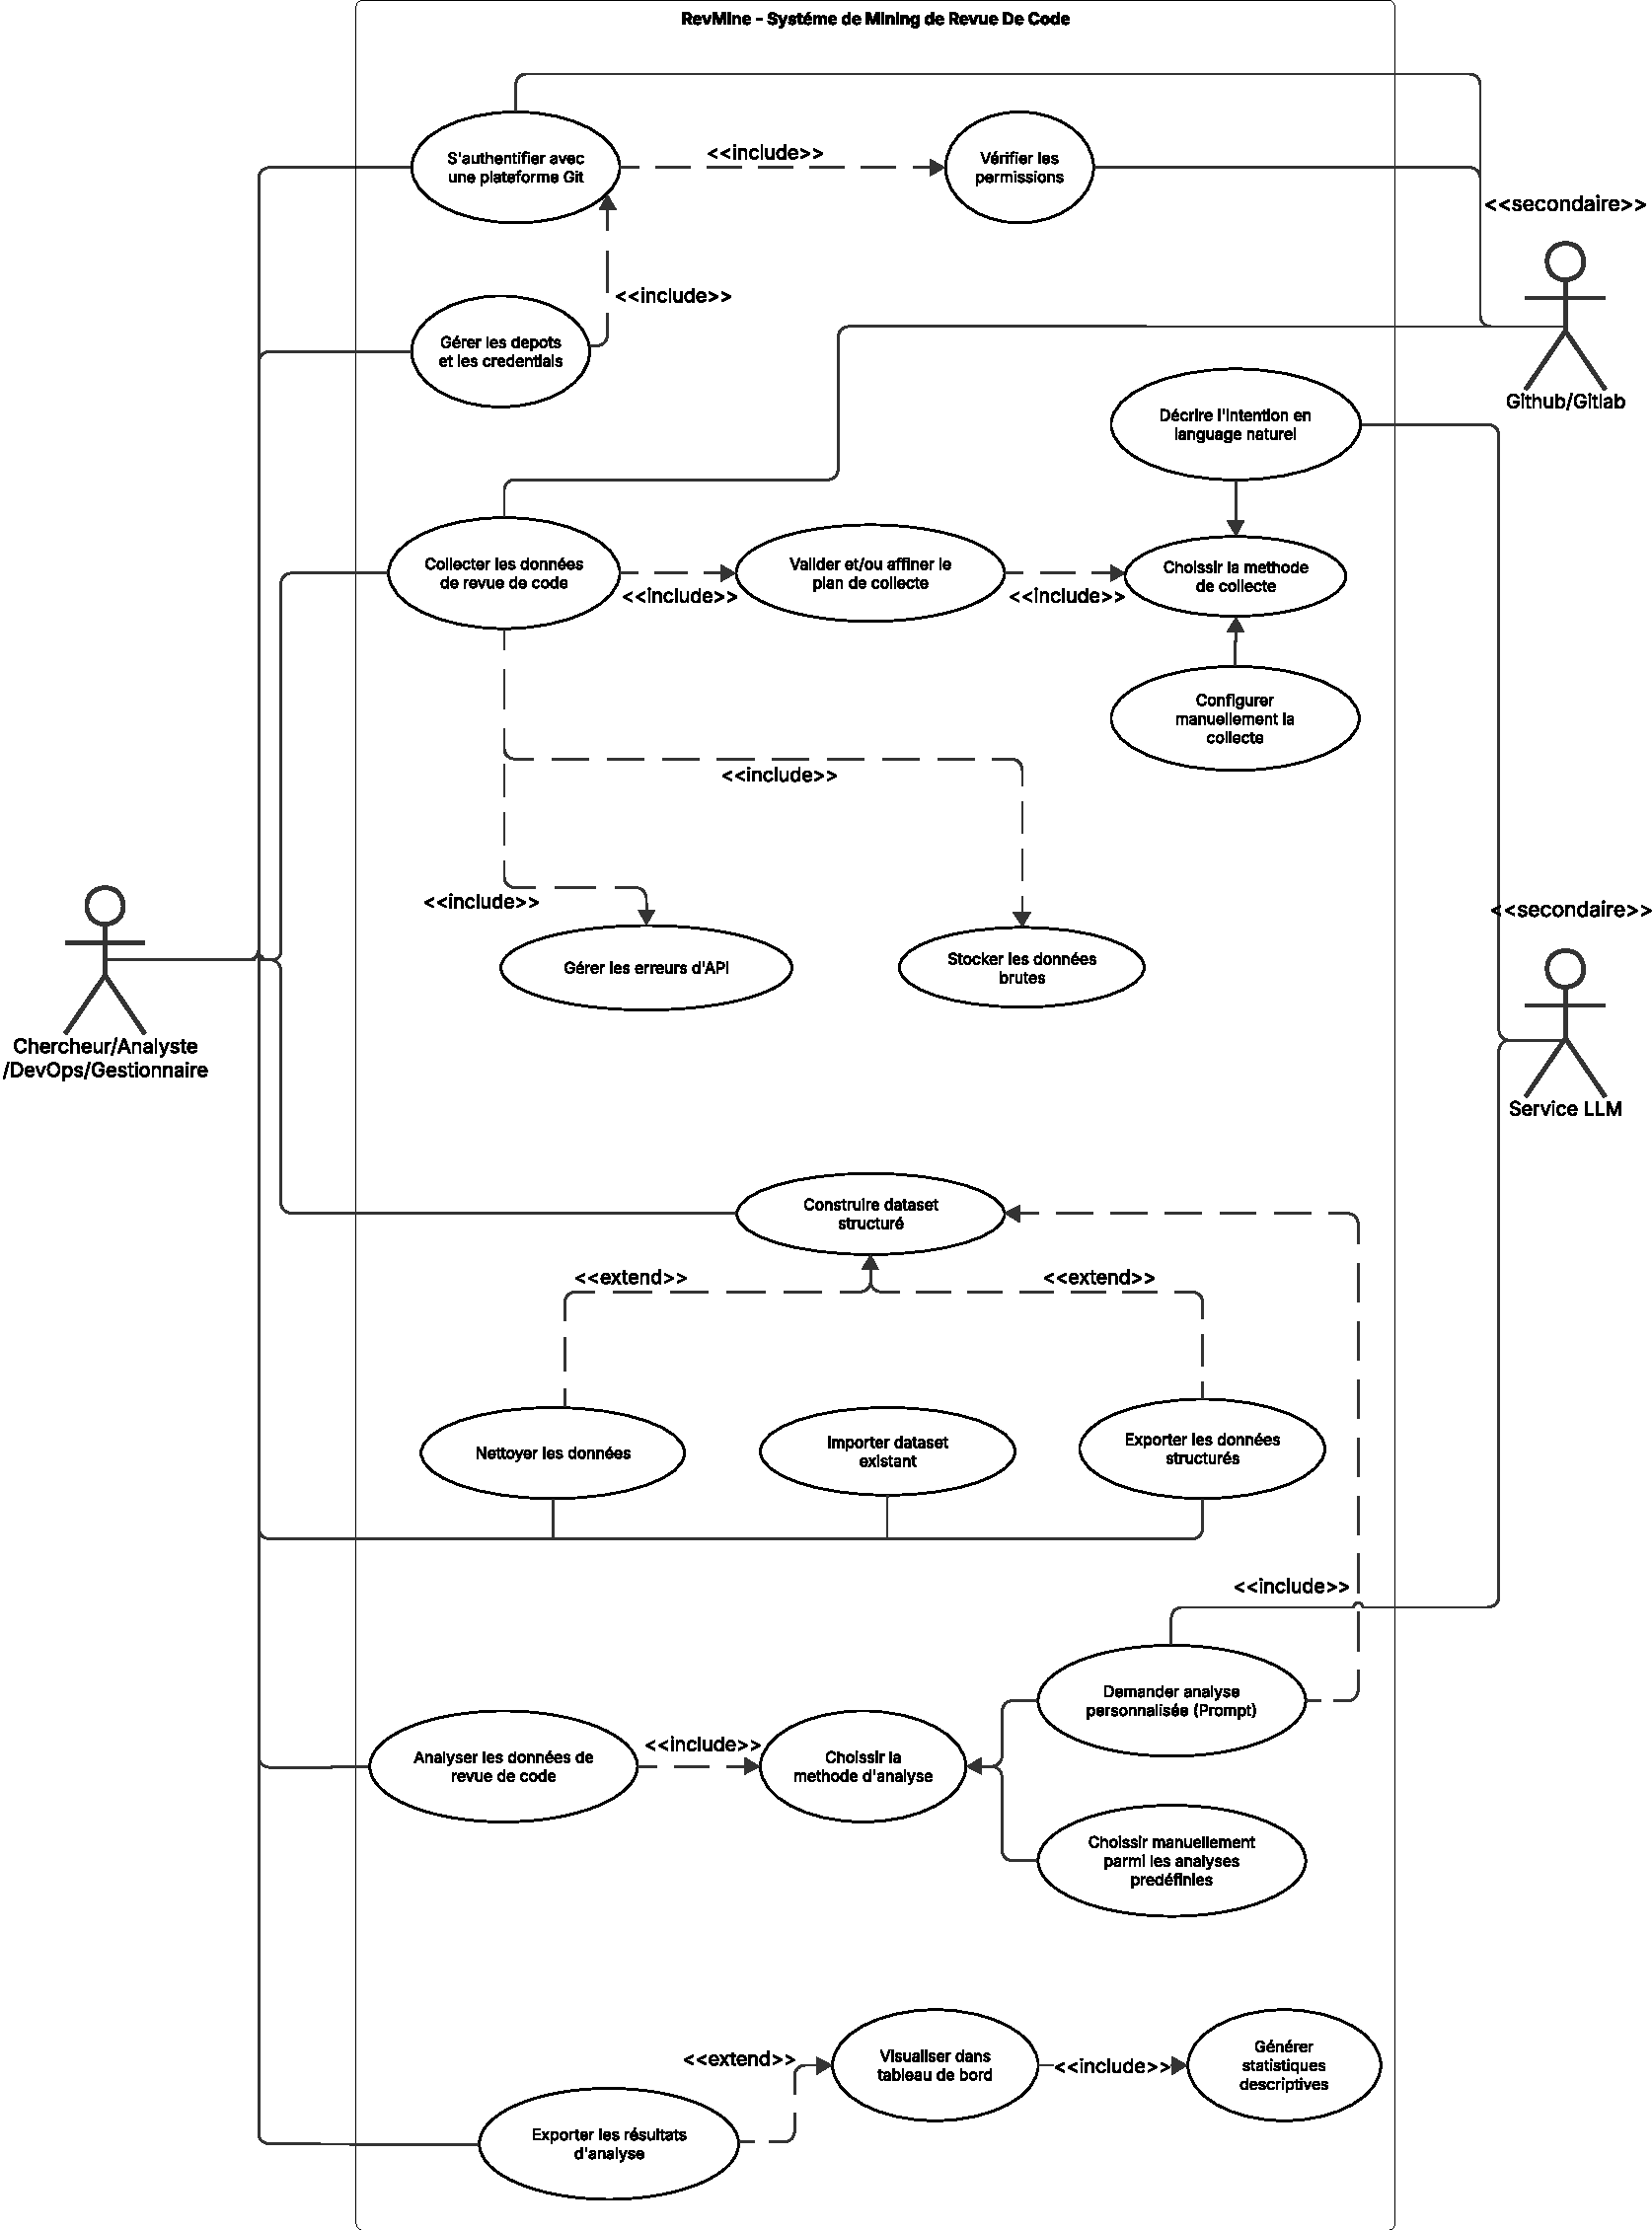
\includegraphics[width=\textwidth]{figures/useCaseDiagramm.pdf}
            \caption{Diagramme de cas d’utilisation}
            \label{fig:diagramme_cas_utilisation}
        \end{figure}

\subsection{Documentation des cas d'utillisation}
Parmi l’ensemble des cas d’utilisation identifiés, deux fonctionnalités principales se distinguent par leur rôle central dans le système RevMine : la collecte et l’analyse des données. Dans ce qui suit, nous présentons une description détaillée de ces cas d’utilisation, en précisant leurs acteurs, leurs préconditions ainsi que les différents scénarios d’exécution.


\subsubsection*{Cas d'utillisation de collecte des données de revue}
La collecte des données constitue une étape centrale du système RevMine. Après l’importation d’un dépôt depuis GitHub ou GitLab, l’utilisateur configure les paramètres de collecte en sélectionnant les endpoints et les filtres associés (branche, plage temporelle, état des PR/MR), ou en exprimant directement ses besoins en langage naturel afin de générer automatiquement un plan de collecte.

Ce plan est ensuite présenté à l’utilisateur, qui peut le valider ou l’ajuster avant son exécution. Une fois la collecte lancée, le système extrait les données via les API des plateformes et les sauvegarde sous un format structuré, en vue de leur exploitation dans les phases d’analyse.

\begin{tabularx}{\textwidth}{|l|X|}
\hline

\textbf{Nom du cas d’utilisation :} & Collecter les données de revue de code \\ \hline
\textbf{ID :} & UC1 \\ \hline

\textbf{Description :} & 
Ce cas d’utilisation décrit le processus permettant à un utilisateur de collecter les données de revue de code à partir d’un projet GitHub ou GitLab. \\ \hline

\textbf{Acteurs primaires :} & Chercheur / Analyste / DevOps / Gestionnaire \\ \hline
\textbf{Acteurs secondaires :} & API GitHub / GitLab \\ \hline

\textbf{Préconditions :} & 
\begin{itemize}
    \item L’utilisateur est authentifié sur la plateforme cible
    \item Le dépôt à analyser est importé dans l’espace de travail
\end{itemize} \\ \hline

\textbf{Enchaînement principal :} & 
\begin{enumerate}
    \item L’utilisateur sélectionne le dépôt à analyser
    \item Le système propose deux modes de collecte :
    \begin{itemize}
        \item Configuration manuelle
        \item Collecte via un prompt en langage naturel
    \end{itemize}

    \item \textbf{Cas 1 : Configuration manuelle}
    \begin{itemize}
        \item L’utilisateur sélectionne la branche cible (par défaut : \textit{main})
        \item L’utilisateur choisit les endpoints à interroger
        \item L’utilisateur définit la fenêtre temporelle (date de début et date de fin)
        \item L’utilisateur sélectionne le type de PR/MR (open, closed, merged)
        \item L’utilisateur lance la collecte
    \end{itemize}

    \item \textbf{Cas 2 : Collecte via prompt}
    \begin{itemize}
        \item L’utilisateur exprime ses besoins de collecte en langage naturel
        \item Le système génère automatiquement un plan de collecte
    \end{itemize}

    \item Le système affiche le plan de collecte généré
    \item L’utilisateur peut valider ou modifier les paramètres (branche, endpoints, filtres, etc.)
    \item Une fois validée, la collecte est lancée
    \item Le système extrait les données via les API et les sauvegarde sous forme structurée
\end{enumerate} \\ \hline

\textbf{Postconditions :} & 
\begin{itemize}
    \item Les données de revue de code sont collectées et stockées
    \item Des statistiques générales sur les données collectées peuvent être affichées
    \item L’utilisateur peut :
    \begin{itemize}
        \item Mettre en pause ou arrêter la collecte
        \item Télécharger les données brutes
    \end{itemize}
\end{itemize} \\ \hline

\textbf{Scénarios alternatifs :} & 
\begin{itemize}
    \item \textbf{Erreur lors de la collecte :}
    En cas d’erreur (réseau ou API), les données déjà collectées sont sauvegardées. Une notification informe l’utilisateur de l’arrêt du processus, avec possibilité de reprise ultérieure.

    \item \textbf{Modification du plan de collecte :}
    Si le plan généré ne correspond pas aux attentes, l’utilisateur peut le modifier avant validation.
\end{itemize} \\ \hline

\end{tabularx}



\subsubsection*{Cas d'utillisation d'analyse des données de revue de code}

L’analyse des données de revue de code permet d’exploiter les informations collectées afin d’en extraire des indicateurs pertinents. À partir de données préalablement collectées ou importées, et enrichies par le calcul de métriques (lead time, code churn, etc.), l’utilisateur peut explorer et affiner les données à l’aide de filtres tels que les auteurs, les types de fichiers, les plages temporelles ou des mots-clés.

L’analyse peut être réalisée soit à travers des options prédéfinies, soit en exprimant les besoins en langage naturel. Le système génère alors des visualisations interactives et personnalisables, facilitant l’interprétation des résultats et leur exploitation.

\begin{tabularx}{\textwidth}{|l|X|}
\hline

\textbf{Nom du cas d’utilisation :} & Analyser les données de revue de code \\ \hline
\textbf{ID :} & UC2 \\ \hline

\textbf{Description :} & 
Ce cas d’utilisation décrit le processus permettant à un utilisateur d’analyser les données de revue de code collectées. \\ \hline

\textbf{Acteurs primaires :} & Chercheur / Analyste / DevOps / Gestionnaire \\ \hline
\textbf{Acteurs secondaires :} & Service LLM \\ \hline

\textbf{Préconditions :} & 
\begin{itemize}
    \item Les données sont disponibles (collectées ou importées)
    \item Les métriques nécessaires sont calculées, ou un dataset contenant les métriques est fourni
\end{itemize} \\ \hline

\textbf{Enchaînement principal :} & 
\begin{enumerate}
    \item L’utilisateur sélectionne le dataset à analyser
    \item L’utilisateur peut nettoyer et filtrer les données (auteurs, types de fichiers, plage temporelle, mots-clés, etc.)
    \item L’utilisateur choisit le mode d’analyse :
    \begin{itemize}
        \item Analyse manuelle
        \item Analyse via prompt en langage naturel
    \end{itemize}

    \item \textbf{Cas 1 : Analyse manuelle}
    \begin{itemize}
        \item L’utilisateur sélectionne parmi les analyses prédéfinies (ex. : collaboration, performance des contributeurs, évolution des métriques, etc.)
        \item Le système génère des visualisations et des graphiques adaptés
        \item L’utilisateur explore les résultats à travers ces visualisations
        \item Les graphiques sont ajustables et personnalisables selon les besoins
    \end{itemize}

    \item \textbf{Cas 2 : Analyse via prompt}
    \begin{itemize}
        \item L’utilisateur exprime son besoin en langage naturel
        \item Le système génère automatiquement des visualisations correspondant à la demande
    \end{itemize}
\end{enumerate} \\ \hline

\textbf{Postconditions :} & 
\begin{itemize}
    \item Les résultats d’analyse sont affichés sous forme de tableaux de bord et de graphiques
    \item Des statistiques générales sont générées
    \item L’utilisateur peut exporter les résultats
    \item L’historique des analyses est accessible
\end{itemize} \\ \hline

\textbf{Scénarios alternatifs :} & 
\begin{itemize}
    \item \textbf{Métriques manquantes :}
    Si certaines analyses ne peuvent être réalisées en raison de l’absence de métriques, le système propose de les calculer à partir des données brutes disponibles.
\end{itemize} \\ \hline

\end{tabularx}

\newpage
\subsection{Diagrammes d'activité}
Afin de compléter la modélisation des cas d’utilisation, des diagrammes d’activité sont proposés pour illustrer le déroulement des principaux processus du système. Ces diagrammes permettent de représenter de manière dynamique les différentes étapes ainsi que les enchaînements des actions réalisées lors de l’exécution des fonctionnalités clés.

\subsubsection*{Configuration de Collecte des Données}
 \begin{figure}[H]
            \centering
            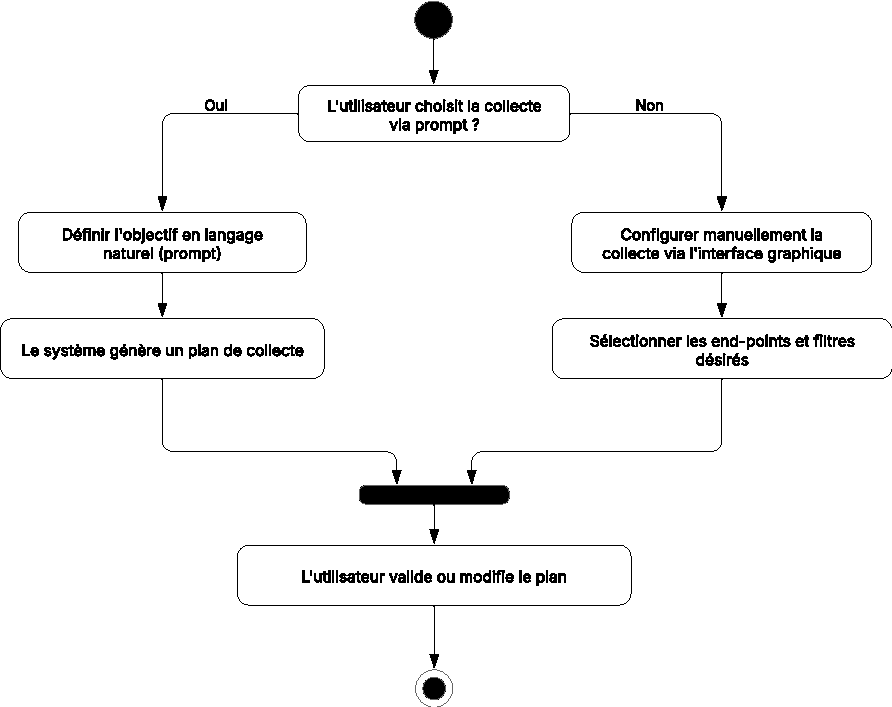
\includegraphics[width=\textwidth]{figures/Diagramme_activite2.pdf}
            \caption{Diagramme d’activité – Création et validation du plan de collecte.}
            \label{fig:activite_collecte_configuration}
        \end{figure}

\subsubsection*{Post-Collecte des Données}
\begin{figure}[H]
    \centering
    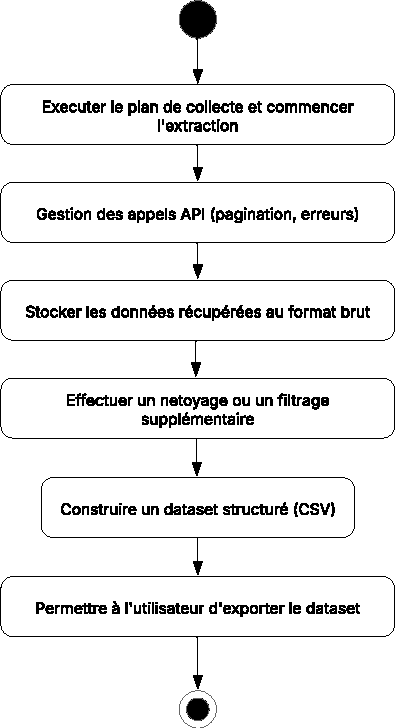
\includegraphics[height=18cm, keepaspectratio]{figures/Diagramme_activite1.pdf}
    \caption{Diagramme d’activité – Filtrage et Nettoyage des données collectées.}
    \label{fig:activite_post_collecte}
\end{figure}

\subsubsection*{L'Analyse des Données}
 \begin{figure}[H]
            \centering
            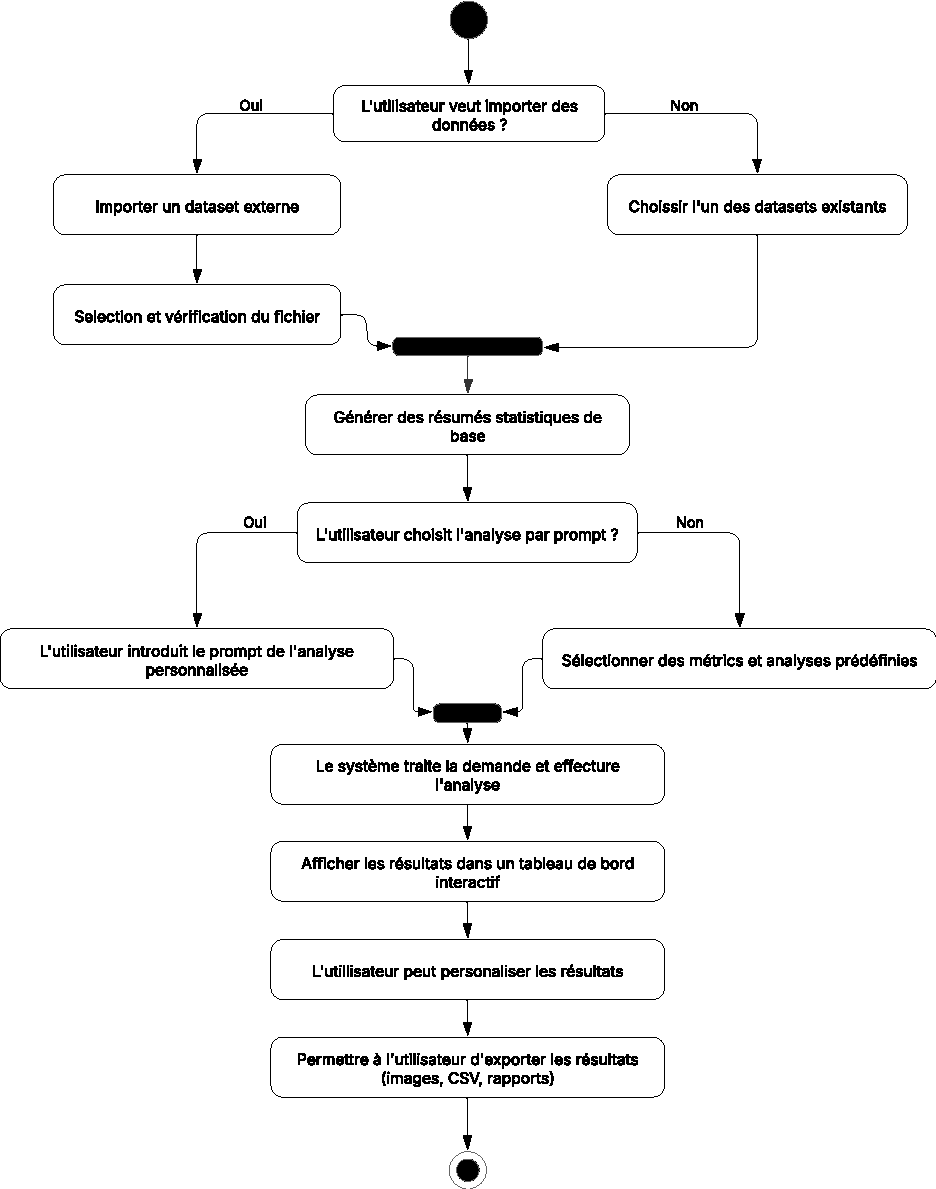
\includegraphics[width=\textwidth]{figures/Diagramme_activite3.pdf}
            \caption{Diagramme d’activité – Configuration, exécution et visualisation des analyses.}
            \label{fig:activite_analyse_donnees}
        \end{figure}




\section{Traçabilité des besoins}
Afin d’assurer la cohérence entre les besoins fonctionnels identifiés et la modélisation du système, une matrice de traçabilité est établie. Elle permet de vérifier que chaque cas d’utilisation couvre bien un ou plusieurs besoins fonctionnels.

\begin{tabularx}{\textwidth}{|l|X|}
\hline

\textbf{Cas d’utilisation} & \textbf{Besoins fonctionnels couverts} \\ \hline

S’authentifier avec une plateforme Git & BF2, BF3, BF4 \\ \hline
Vérifier les permissions & BF4 \\ \hline
Gérer les dépôts et les credentials & BF1, BF2, BF3, BF5 \\ \hline
Collecter les données de revue de code & BF5, BF6, BF7, BF8, BF9, BF10, BF11 \\ \hline
Choisir la méthode de collecte & BF6, BF7 \\ \hline
Configurer manuellement la collecte & BF6 \\ \hline
Décrire l’intention en langage naturel & BF7 \\ \hline
Valider et/ou affiner le plan de collecte & BF8 \\ \hline
Gérer les erreurs d’API & BF10 \\ \hline
Stocker les données brutes & BF11 \\ \hline
Construire dataset structuré & BF11, BF12, BF13, BF14, BF20 \\ \hline
Nettoyer les données & BF12 \\ \hline
Importer dataset existant & BF13 \\ \hline
Exporter les données structurées & BF20 \\ \hline
Analyser les données de revue de code & BF14, BF15, BF16, BF17, BF18, BF19, BF20 \\ \hline
Choisir la méthode d’analyse & BF15, BF16 \\ \hline
Demander analyse personnalisée (Prompt) & BF15 \\ \hline
Choisir manuellement parmi les analyses prédéfinies & BF16 \\ \hline
Visualiser dans tableau de bord & BF17, BF18, BF19 \\ \hline
Générer statistiques descriptives & BF18 \\ \hline
Exporter les résultats d’analyse & BF20 \\ \hline

\end{tabularx}




\section{Conclusion}
Ce chapitre a permis d’établir les fondements analytiques de la solution RevMine à travers une étude structurée des besoins. Nous avons tout d’abord présenté la méthodologie suivie, puis identifié les différents acteurs du système avant de définir les besoins fonctionnels et non fonctionnels.

Ces besoins ont ensuite été validés afin d’assurer leur cohérence et leur adéquation avec les objectifs du projet, aussi bien du point de vue académique qu’industriel. Par la suite, ils ont été modélisés à travers un diagramme de cas d’utilisation, une documentation des cas principaux, des diagrammes d’activité ainsi qu’une matrice de traçabilité permettant de vérifier leur couverture.

Cette analyse constitue ainsi un socle solide pour la suite du développement. Dans le chapitre suivant, nous aborderons la phase de conception, où les besoins identifiés seront traduits en une architecture détaillée et en choix de conception permettant de structurer la solution proposée.


\chapter{Spécification des données, métriques et analyses retenues}
\section{Introduction}

Dans le cadre de RevMine, l’analyse des données de revue de code repose sur l’identification d’un ensemble de données, de métriques et d’analyses permettant de mieux comprendre les dynamiques du processus de revue. L’objectif est de transformer les informations extraites depuis les plateformes GitHub et GitLab en indicateurs exploitables pour les chercheurs, les praticiens DevOps et les managers.

Ce chapitre présente les données retenues dans la plateforme RevMine. Nous commençons par définir les informations générales extraites des PR/MR, qui constituent la base nécessaire au calcul des métriques. Ensuite, nous présentons les différentes catégories de métriques retenues, puis les analyses et visualisations proposées à partir de ces indicateurs.


\section{Critères de sélection des métriques}

La sélection des métriques intégrées dans RevMine s’appuie sur trois critères principaux :

\begin{itemize}
    \item \textbf{Pertinence scientifique :} les métriques retenues sont alignées avec les indicateurs couramment utilisés dans les études empiriques sur la revue de code, notamment les mesures temporelles, les métriques de collaboration, les métriques liées aux changements de code et les mesures d’interaction dans les discussions \cite{chouchen2023reviewcompletion,bosu2014developerreputation,bavota2015four,rahman2017revhelper,turzo2023usefulcomments}.

    \item \textbf{Exploitabilité multi-plateformes :} les métriques doivent pouvoir être calculées à partir des données disponibles sur GitHub et GitLab, malgré les différences entre leurs modèles de données. Les plateformes fournissent notamment des informations sur les PR/MR, les commits, les commentaires, les fichiers modifiés et les décisions de revue \cite{kansab2025revmine,kansab2025devopsmr}.

    \item \textbf{Capacité d’analyse :} les métriques doivent permettre de produire des visualisations et analyses utiles pour les chercheurs, les praticiens DevOps et les managers, en facilitant l’identification des retards, des contributions importantes, de la complexité des changements ou des anomalies dans le processus de revue \cite{chouchen2023reviewcompletion,hassan2009predicting,kansab2025devopsmr}.
\end{itemize}

Certaines métriques, telles que le \textit{code churn}, l’entropie historique ou la diversité des committers, ne sont pas directement fournies comme métriques prêtes à l’emploi par les API. Elles doivent être calculées en combinant plusieurs champs collectés, ce qui justifie la nécessité d’un catalogue structuré de données et de métriques \cite{hassan2009predicting,bavota2015four,thongtanunam2015reviewer}.

\section{Données générales collectées}
Avant de calculer les métriques, RevMine doit extraire un ensemble d’informations générales relatives aux projets, aux dépôts et aux PR/MR. Ces informations ne sont pas toujours considérées comme des métriques d’analyse à part entière, mais elles sont indispensables pour identifier les entités collectées, structurer les datasets et calculer les indicateurs avancés.

\begin{table}[H]
\centering
\begin{tabular}{|p{3.5cm}|p{5cm}|p{6cm}|}
\hline
\textbf{Donnée} & \textbf{Description} & \textbf{Utilisation} \\
\hline
\textbf{Project ID} & Identifiant du projet ou dépôt analysé & Permet de rattacher chaque PR/MR à son projet d’origine \\
\hline
\textbf{Repository Name} & Nom du dépôt analysé & Facilite l’identification du projet dans les datasets \\
\hline
\textbf{Platform} & Plateforme source : GitHub ou GitLab & Permet de distinguer l’origine des données \\
\hline
\textbf{PR/MR ID} & Identifiant unique de la Pull Request ou Merge Request & Permet d’identifier chaque unité de revue \\
\hline
\textbf{PR/MR Title} & Titre de la PR/MR & Peut être utilisé pour des analyses textuelles ou des filtres par mots-clés \\
\hline
\textbf{PR/MR Description} & Description associée à la PR/MR & Sert à comprendre le contexte de la modification \\
\hline
\textbf{Author} & Auteur ayant créé la PR/MR & Utilisé pour les analyses de contribution \\
\hline
\textbf{Created At} & Date de création de la PR/MR & Sert au calcul des métriques temporelles \\
\hline
\textbf{Updated At} & Date de dernière mise à jour & Permet de suivre l’évolution de la PR/MR \\
\hline
\textbf{Merged At} & Date de fusion, si applicable & Sert au calcul du lead time \\
\hline
\textbf{Closed At} & Date de fermeture, si applicable & Permet d’analyser les PR/MR non fusionnées \\
\hline
\textbf{State} & État de la PR/MR : ouverte, fermée ou fusionnée & Permet d’analyser l’issue des contributions \\
\hline
\textbf{Source Branch} & Branche source de la PR/MR & Donne le contexte de développement \\
\hline
\textbf{Target Branch} & Branche cible de la PR/MR & Permet d’identifier la branche d’intégration \\
\hline
\textbf{Labels} & Labels associés à la PR/MR & Permettent des analyses par catégorie ou priorité \\
\hline
\textbf{URL} & Lien vers la PR/MR sur la plateforme source & Facilite la traçabilité des données collectées \\
\hline
\end{tabular}
\end{table}

Ces données permettent de conserver la traçabilité des éléments collectés et servent d’entrée au calcul des métriques temporelles, collaboratives et liées au code.



\section{Métriques utilisées}

Les métriques sélectionnées dans RevMine sont organisées en plusieurs catégories afin de faciliter leur interprétation.

\subsection{Métriques temporelles}

\begin{table}[H]
\centering
\begin{tabular}{|l|p{5cm}|p{6cm}|}
\hline
\textbf{Métrique} & \textbf{Description} & \textbf{Justification} \\
\hline
Lead Time & Temps entre la création et la fermeture (ou fusion) d’une PR/MR & Indicateur clé de performance DevOps permettant d’évaluer la rapidité du processus de revue \\
\hline
Temps moyen entre commits & Intervalle moyen entre deux commits successifs & Permet d’analyser le rythme de développement et l’activité des contributeurs \\
\hline
Delta Time & Temps entre la création du projet et la création de la PR/MR & Donne un contexte temporel sur la maturité du projet \\
\hline
\end{tabular}
\caption{Métriques temporelles}
\end{table}

\subsection{Métriques de collaboration}

\begin{table}[H]
\centering
\begin{tabular}{|l|p{5cm}|p{6cm}|}
\hline
\textbf{Métrique} & \textbf{Description} & \textbf{Justification} \\
\hline
Nombre de commentaires & Total des commentaires dans la PR/MR & Reflète le niveau d’interaction et la profondeur de la revue \\
\hline
Nombre de discussions & Nombre de threads de discussion & Permet d’évaluer la complexité des échanges \\
\hline
Nombre de réviseurs & Nombre de personnes impliquées dans la revue & Indique le niveau de collaboration et de validation \\
\hline
Nombre de participants & Nombre total d’acteurs impliqués & Mesure globale de la collaboration \\
\hline
Nombre de committers & Nombre de contributeurs ayant effectué des commits & Permet d’analyser la distribution du travail \\
\hline
Auteurs majeurs / mineurs & Classification des contributeurs selon leur contribution & Permet d’identifier la concentration ou la dispersion du travail \\
\hline
\end{tabular}
\caption{Métriques de collaboration}
\end{table}

\subsection{Métriques de code}

\begin{table}[H]
\centering
\begin{tabular}{|p{4cm}|p{5cm}|p{6cm}|}
\hline
\textbf{Métrique} & \textbf{Description} & \textbf{Justification} \\
\hline
Code churn (additions/suppressions) & Nombre total de lignes ajoutées et supprimées & Indicateur de l’effort de développement et de la taille des modifications \\
\hline
Nombre de fichiers modifiés & Total des fichiers impactés & Permet d’évaluer la portée des changements \\
\hline
Types de fichiers & Nombre de types de fichiers modifiés & Indique la diversité technique des modifications \\
\hline
Taille initiale & Taille des modifications avant la création de la PR/MR & Donne une idée de la préparation du travail \\
\hline
Rework size & Modifications effectuées après les retours de revue & Indicateur de l’effort de correction suite aux feedbacks \\
\hline
Entropie historique & Mesure de la dispersion des modifications dans le code & Permet d’évaluer la complexité et la dispersion des changements \\
\hline
\end{tabular}
\caption{Métriques liées au code}
\end{table}

\subsection{Métriques générales}

\begin{table}[H]
\centering
\begin{tabular}{|l|p{5cm}|p{6cm}|}
\hline
\textbf{Métrique} & \textbf{Description} & \textbf{Justification} \\
\hline
Nombre de commits & Total des commits dans la PR/MR & Indicateur de granularité des modifications \\
\hline
État de la PR/MR & Statut (ouverte, fusionnée, fermée) & Permet d’analyser l’issue des contributions \\
\hline
\end{tabular}
\caption{Métriques générales}
\end{table}

\section{Analyses proposées}

À partir des données collectées et des métriques calculées, RevMine propose un ensemble d’analyses permettant d’explorer les pratiques de revue de code. Ces visualisations facilitent l’interprétation des résultats et permettent d’identifier des tendances ou anomalies dans les projets étudiés.

\begin{table}[H]
\centering
\begin{tabular}{|p{4cm}|p{5cm}|p{6cm}|}
\hline
\textbf{Analyse} & \textbf{Description} & \textbf{Justification} \\
\hline
Commits over time & Évolution du nombre de commits dans le temps & Permet d’identifier les périodes d’activité intense \\
\hline
Timeline des PR/MR & Distribution temporelle des créations de PR/MR & Donne une vision globale de l’activité du projet \\
\hline
Distribution du lead time & Répartition des temps de revue & Permet d’identifier les retards ou inefficacités \\
\hline
Distribution des commits & Répartition du nombre de commits par PR/MR & Analyse la granularité du travail \\
\hline
Analyse des committers & Contribution des différents développeurs & Permet d’identifier les principaux contributeurs \\
\hline
Code churn & Analyse des ajouts et suppressions de code & Évalue l’effort de développement \\
\hline
Analyse des discussions & Étude des interactions dans les PR/MR & Permet d’évaluer la qualité des échanges \\
\hline
Analyse des fichiers modifiés & Distribution des fichiers impactés & Donne une idée de la portée des modifications \\
\hline
Distribution des types de fichiers & Répartition des extensions de fichiers & Permet d’identifier les technologies dominantes \\
\hline
Analyse d’entropie & Mesure de la dispersion des changements & Évalue la complexité des modifications \\
\hline
Matrice de corrélation & Relations entre différentes métriques & Permet d’identifier des dépendances entre variables \\
\hline
Analyse de complexité des PR/MR & Évaluation globale de la complexité & Fournit une vue synthétique du travail effectué \\
\hline
Top contributeurs & Classement des auteurs, reviewers et committers & Permet d’identifier les acteurs clés du projet \\
\hline
\end{tabular}
\caption{Analyses proposées dans RevMine}
\end{table}

\section{Conclusion}

Les données, métriques et analyses retenues permettent de structurer la logique analytique de RevMine. Les informations générales assurent l’identification et la traçabilité des PR/MR collectées, tandis que les métriques fournissent des indicateurs quantitatifs sur le temps, la collaboration et la complexité des changements.

Les analyses proposées exploitent ces métriques afin de générer des visualisations et des résultats interprétables par les utilisateurs. Ce chapitre constitue ainsi la base fonctionnelle du service de collecte et du service d’analyse, qui seront détaillés dans les chapitres de conception et de réalisation.

\chapter{Conception}

\section{Introduction}

À la suite de l’analyse des besoins, la phase de conception vise à établir la structure logique et le fonctionnement global du système. Elle traduit les exigences fonctionnelles et non fonctionnelles en une architecture cohérente, mettant en évidence les principaux composants, leurs interactions et les flux d’informations qui les relient. Cette étape garantit que la solution répond aux attentes des utilisateurs tout en respectant les contraintes de performance, de fiabilité et de sécurité. Les modèles UML présentés dans cette section (cas d’utilisation, activités, classes et séquences) reflètent les choix de conception effectués en vue de la réalisation de la plateforme.


\section{Objectifs de conception}
La conception de RevMine vise à proposer une solution capable de regrouper l’ensemble du processus d’analyse des données de revue de code dans une plateforme accessible, efficace et conviviale. Les objectifs retenus orientent les choix architecturaux et permettent d’assurer l’adéquation entre les besoins identifiés et la solution proposée.

\vspace{0.5cm}

\begin{tabularx}{\textwidth}{|l|X|}
\hline
\textbf{Objectif} & \textbf{Description} \\ \hline

\textbf{Accessibilité} & Permettre à différents profils d’utilisateurs, notamment les chercheurs, praticiens DevOps et managers, d’exploiter les données de revue de code sans nécessiter une expertise avancée en programmation ou en manipulation d’API. \\ \hline

\textbf{Modularité} & Séparer les principales responsabilités du système en modules indépendants, tels que la gestion des espaces de travail, la collecte, l’analyse et la visualisation, l’interaction avec les modèles de langage. \\ \hline

\textbf{Maintenabilité} & Faciliter l’évolution et la correction du système en permettant la modification d’un module sans impacter l’ensemble de la plateforme. \\ \hline

\textbf{Extensibilité} & Permettre l’ajout progressif de nouvelles plateformes, métriques, analyses et modèles LLM afin d’adapter RevMine à l’évolution rapide du domaine. \\ \hline

\textbf{Fiabilité} & Garantir une collecte correcte et robuste des données, en limitant les risques d’erreurs, de pertes de données ou d’interruptions non maîtrisées. \\ \hline

\textbf{Réutilisabilité des données} & Conserver les données collectées et l’historique des opérations afin d’éviter les collectes répétées et de permettre des analyses ultérieures. \\ \hline

\textbf{Sécurité} & Assurer la protection des informations sensibles, notamment les tokens d’accès aux plateformes Git ainsi que les données collectées à partir des projets. \\ \hline

\textbf{Flexibilité} & Offrir à l’utilisateur la possibilité d’utiliser différents fournisseurs de modèles de langage, y compris des modèles locaux, afin de répondre aux contraintes de confidentialité, de coût ou de performance. \\ \hline

\end{tabularx}

\vspace{0.5cm}

Ces objectifs constituent la base des décisions de conception adoptées pour RevMine.


\section{Architecture générale}
\subsection{Étude comparative des styles architecturaux}

Les architectures logicielles contemporaines les plus répandues incluent les approches monolithique, modulaire, microservices et serverless. Chacune présente des compromis entre flexibilité, complexité et performance. Le Tableau suivant résume les principales caractéristiques de ces modèles architecturaux selon la littérature récente.



\begin{table}[H]
\centering
\small
\begin{tabularx}{\textwidth}{|l|Y|Y|Y|Y|Y|}
\hline
\textbf{Architecture} & \textbf{Scalabilité} & \textbf{Extensibilité} & \textbf{Résilience} & \textbf{Complexité de déploiement} & \textbf{Cas d’usage typiques} \\
\hline
Monolithique & Faible à moyenne, principalement verticale & Limitée par le couplage interne & Faible à moyenne & Faible & Applications simples, stables ou de petite taille \\
\hline
Modulaire & Moyenne & Moyenne à élevée & Moyenne & Moyenne & Applications structurées en composants fonctionnels séparés \\
\hline
Microservices & Élevée, principalement horizontale & Élevée grâce à l’indépendance des services & Élevée & Élevée & Systèmes distribués, évolutifs et nécessitant plusieurs traitements indépendants \\
\hline
Serverless & Très élevée & Moyenne & Élevée & Moyenne & Traitements ponctuels, événementiels ou temporaires\\
\hline
\end{tabularx}
\caption{Comparaison des principales architectures logicielles selon la littérature.}
\label{tab:comparaison_architectures}
\end{table}

Cette comparaison montre que chaque architecture présente des avantages et des limites selon le contexte d’utilisation. L’architecture monolithique se distingue par sa simplicité de développement et de déploiement, mais elle devient moins adaptée lorsque le système évolue ou lorsque les composants doivent être modifiés indépendamment \cite{richards2015software}. Les architectures modulaires améliorent l’organisation interne du système, mais elles ne garantissent pas toujours une mise à l’échelle indépendante des composants \cite{richards2015software}. Les microservices, quant à eux, permettent de découper le système en services autonomes, faiblement couplés et indépendamment déployables, ce qui favorise la scalabilité, la maintenabilité et l’évolution continue du système \cite{fowler2014microservices,newman2021building}. Fowler et Lewis décrivent les microservices comme des services indépendamment déployables et scalables, avec des frontières modulaires claires \cite{fowler2014microservices}. IBM souligne également que les microservices offrent une meilleure scalabilité que les architectures monolithiques, notamment parce que les services peuvent être mis à l’échelle séparément \cite{ibm2024monolithicMicroservices}. Toutefois, cette approche introduit une complexité plus importante, notamment en matière de coordination, de communication et de gestion globale du système \cite{richards2015software,newman2021building}. Enfin, l’architecture serverless est adaptée aux charges variables et événementielles, mais elle dépend fortement des plateformes cloud et présente encore plusieurs défis techniques, notamment autour de la gestion de l’état et de la prévisibilité des performances \cite{baldini2017serverless}.

\subsection{Choix architectural}

À la suite de la définition des objectifs de conception et de l’étude comparative des principaux styles architecturaux, l’architecture \textbf{Microservices organisée en couches} apparaît comme le choix le plus adapté pour RevMine.

Ce style architectural permet de répondre aux exigences principales du système, notamment la séparation des responsabilités, l’évolutivité, la maintenabilité et l’intégration de composants hétérogènes tels que les services de collecte, d’analyse, de stockage et d’interaction avec les modèles de langage.

Ainsi, ce choix architectural sera retenu pour la conception de RevMine. La section suivante présente les éléments qui justifient plus en détail cette décision.



\subsection{Justification du choix}

Le choix d’une architecture microservices organisée en couches se justifie par la nature même de RevMine, dont les principales fonctionnalités correspondent à des responsabilités distinctes. La gestion des workspaces et des dépôts, la collecte des données, l’analyse des résultats et l’interaction en utilisant le language naturel peuvent être considérées comme des domaines fonctionnels relativement indépendants.

Cette architecture permet ainsi de répondre aux objectifs de conception définis précédemment :

\begin{itemize}
    \item \textbf{Accessibilité} : la séparation entre l’interface utilisateur, les services de traitement et les services d’analyse permet de proposer une plateforme claire et exploitable par différents profils d’utilisateurs.

    \item \textbf{Modularité et maintenabilité} : chaque service porte une responsabilité précise, ce qui facilite son évolution, sa correction ou son remplacement sans affecter l’ensemble du système.

    \item \textbf{Extensibilité} : l’ajout de nouvelles plateformes, métriques, analyses ou modèles LLM peut être réalisé progressivement, en intervenant uniquement sur les services concernés.

    \item \textbf{Fiabilité} : l’isolation des traitements, notamment ceux liés à la collecte des données, permet de mieux gérer les erreurs et de limiter leur impact sur le reste de la plateforme.

    \item \textbf{Réutilisabilité des données} : les données produites par chaque service peuvent être conservées dans son propre espace de persistance, ce qui permet de réutiliser les résultats de collecte, de structuration ou d’analyse sans répéter inutilement les mêmes opérations.
\end{itemize}

Ainsi, l’architecture retenue permet d’aligner la structure technique de RevMine avec sa logique fonctionnelle. Elle offre une base adaptée pour construire une solution évolutive, maintenable et cohérente avec les besoins identifiés.

\section{Vue initiale de l’architecture de RevMine}
La figure ci-dessous présente une vue initiale et simplifiée de l’architecture de RevMine. Elle met en évidence les principales couches de la solution, à savoir la couche de présentation, l’API Gateway, les microservices, la couche de persistance, les services externes ainsi que les mécanismes de communication et de mise en cache. Cette représentation permet d’avoir une première vision globale de l’organisation du système avant de détailler chaque service séparément.
\vspace{1em}
  \begin{figure}[H]
            \centering
            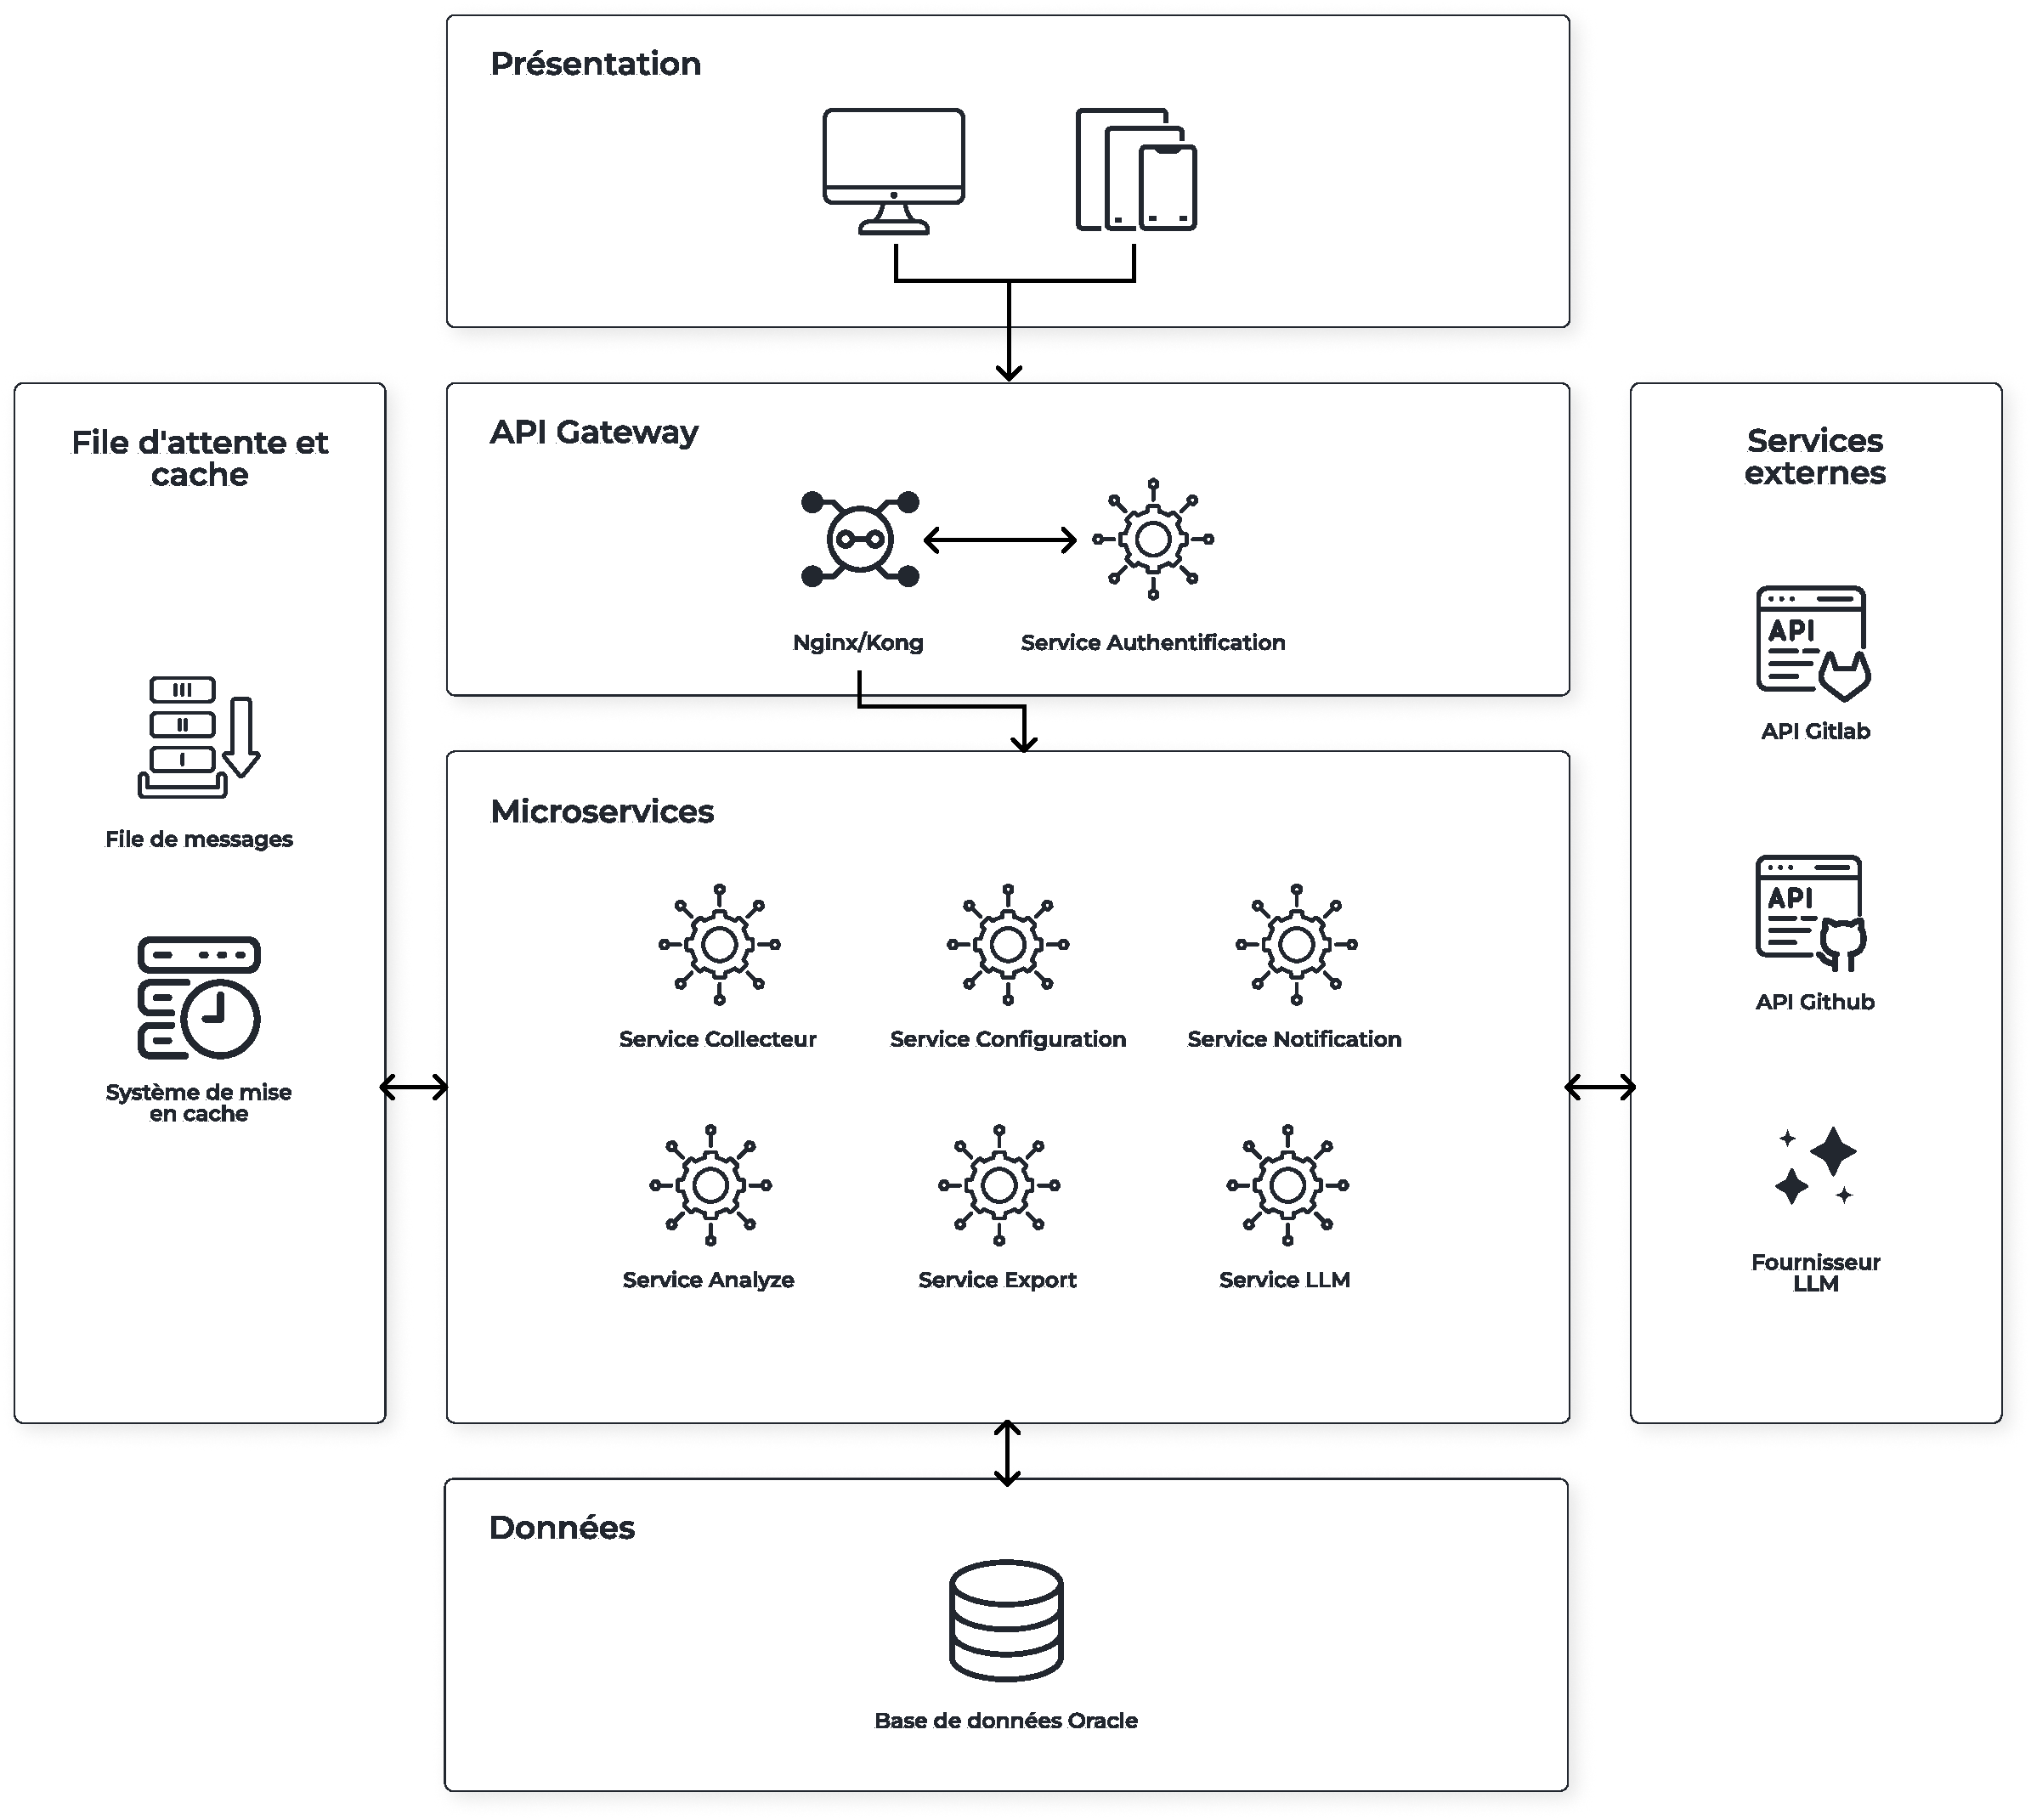
\includegraphics[width=\textwidth]{figures/diagramm_architecture_p.pdf}
            \caption{Schéma simplifié de l’architecture générale de la solution.}
            \label{fig:architecture_generale}
        \end{figure}

\vspace{1em}
L’architecture est structurée autour des éléments suivants :

\begin{itemize}
    \item \textbf{Couche présentation :} elle correspond à l’interface utilisateur de RevMine. Il s’agit d’une interface web intuitive permettant aux utilisateurs d’effectuer les principales opérations offertes par la plateforme, notamment la configuration des projets, le lancement des collectes, l’analyse des données et la consultation des résultats.

    \item \textbf{API Gateway :} cette couche constitue le point d’entrée principal du système. Elle reçoit les requêtes provenant de l’interface utilisateur et les redirige vers les services appropriés. Elle joue également un rôle important dans la gestion de l’authentification et du contrôle d’accès, afin d’assurer que seules les requêtes autorisées soient traitées.

    \item \textbf{Microservices :} cette couche regroupe les services contenant la logique métier de la solution. Chaque service est responsable d’un périmètre fonctionnel précis :
    \begin{itemize}
        \item \textbf{Service de configuration :} permet la connexion aux plateformes GitHub et GitLab, la gestion des tokens, ainsi que l’importation et la gestion des dépôts à analyser.

        \item \textbf{Service collecteur :} prend en charge la configuration et l’exécution des collectes de données de revue de code. Il gère également les opérations associées aux données collectées, telles que le nettoyage, le filtrage, l’historique des collectes et des traitements, ainsi que le calcul des métriques nécessaires à l’analyse.

        \item \textbf{Service d’analyse :} permet d’exploiter les données collectées et les métriques calculées afin de produire différentes analyses, statistiques et visualisations.

        \item \textbf{Service LLM :} assure l’intégration de l’interaction en langage naturel, notamment pour assister l’utilisateur dans la définition des plans de collecte et des analyses.

        \item \textbf{Service de notification :} informe l’utilisateur de l’état des opérations importantes, telles que le démarrage, la progression, la fin ou l’échec d’une collecte ou d’une analyse.

    \end{itemize}

    \item \textbf{Couche données :} bien qu’elle soit représentée de manière regroupée dans le diagramme, cette couche ne correspond pas à une base de données centralisée unique. Dans l’architecture de RevMine, chaque service dispose de sa propre persistance selon ses besoins. En complément, un mécanisme de stockage dédié permet de gérer les fichiers volumineux, tels que les données brutes collectées ou les datasets structurés.

    \item \textbf{Services externes :} RevMine interagit avec des systèmes externes, notamment les API GitHub et GitLab pour l’extraction des données de revue de code, ainsi qu’avec des fournisseurs LLM ou des modèles locaux pour le traitement des requêtes en langage naturel.

    \item \textbf{File d’attente et cache :} ces mécanismes facilitent la communication entre les services, notamment pour les traitements asynchrones ou de longue durée. Ils permettent également d’améliorer la réactivité du système et de mieux gérer certaines opérations répétitives ou coûteuses.
\end{itemize}

Cette vue initiale constitue ainsi une première abstraction de l’architecture de RevMine. Les sections suivantes détaillent la conception interne des différents services afin de mieux comprendre leur structure, leurs responsabilités et les données qu’ils manipulent.

\section{Conception détaillée de l'API Gateway}
L’API Gateway constitue le point d’entrée principal de RevMine. Elle reçoit les requêtes provenant de l’interface utilisateur et les redirige vers les services appropriés. Elle assure également la gestion des utilisateurs, l’authentification, les sessions et la validation des tokens d’accès.

Ce composant joue donc un rôle organisationnel et sécuritaire essentiel, en garantissant la coordination entre l’interface et les différents services métiers.

\begin{table}[H]
\centering
\begin{tabular}{|p{4cm}|p{10cm}|}
\hline
\textbf{Élément} & \textbf{Description} \\
\hline
Entrées & Requêtes utilisateur provenant de l’interface web, informations d’authentification, demandes de routage vers les services. \\
\hline
Sorties & Réponses renvoyées à l’interface utilisateur, tokens de session, requêtes transmises aux services concernés. \\
\hline
Rôle principal & Centraliser l’accès à la plateforme, gérer l’authentification et router les requêtes vers les services métiers. \\
\hline
\end{tabular}
\end{table}

\subsubsection*{Diagramme de classes de l’API Gateway}

Ce diagramme présente les classes liées à la gestion des utilisateurs, des sessions et de l’authentification.
\begin{figure}[H]
\centering
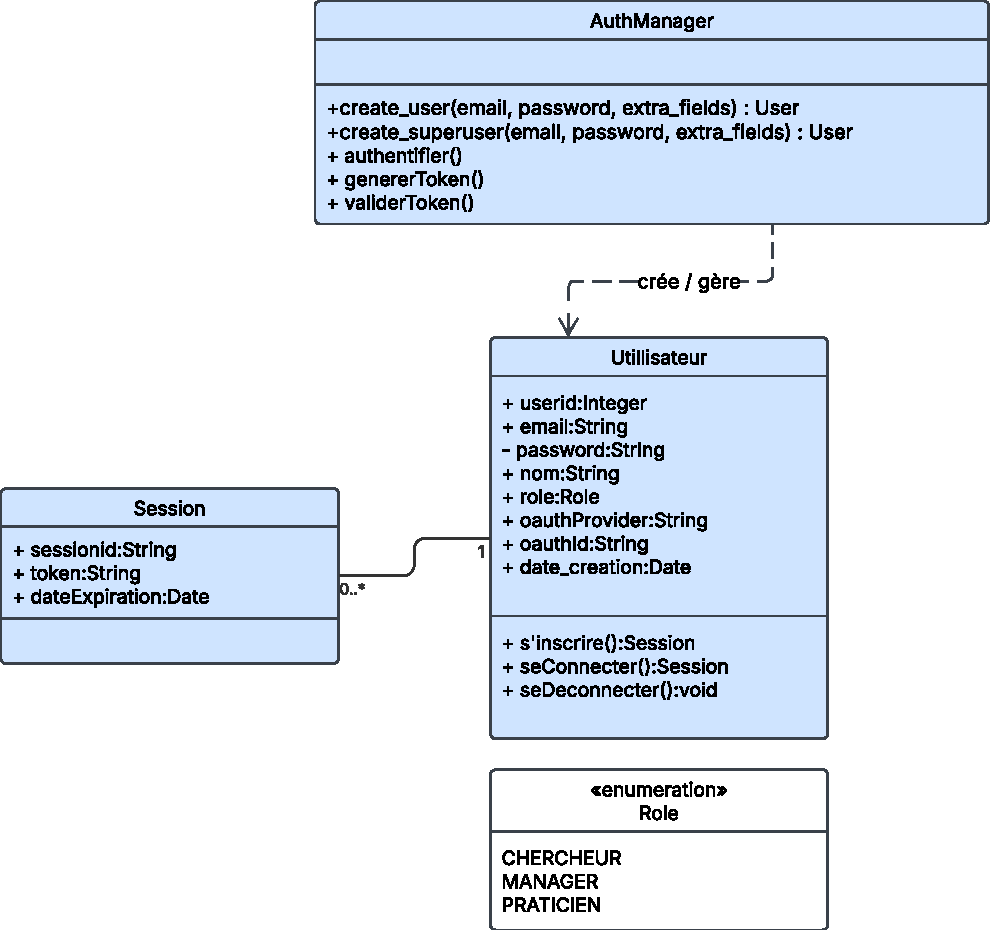
\includegraphics[width=0.9\textwidth]{classDiagramm1.pdf}
\caption{Diagramme de classes de l’API Gateway}
\label{fig:classDiagramm1}
\end{figure}

\section{Conception détaillée des services}
Cette section présente la conception détaillée des principaux services de RevMine. Pour chaque service, nous décrivons son rôle, sa logique fonctionnelle, ses entrées et sorties, ainsi que les besoins fonctionnels auxquels il contribue. Chaque sous-section est complétée par un diagramme de classes et un schéma de base de données afin de préciser la structure interne du service.


\subsection{Service de configuration}

Le service de configuration prépare l’environnement de travail nécessaire aux collectes et aux analyses. Il permet de connecter RevMine aux plateformes GitHub et GitLab, de gérer les tokens d’accès et d’importer les dépôts à analyser.

Les dépôts sont organisés dans des workspaces, ce qui facilite leur gestion, leur sélection et les opérations ultérieures. Ce service assure ainsi la liaison entre RevMine et les plateformes de collaboration logicielle.

\begin{table}[H]
\centering
\begin{tabular}{|p{4cm}|p{10cm}|}
\hline
\textbf{Élément} & \textbf{Description} \\
\hline
\textbf{Entrées} & Tokens d’accès, informations de connexion, paramètres du workspace, dépôts à importer. \\
\hline
\textbf{Sorties} & Workspaces configurés, dépôts importés, métadonnées nécessaires aux collectes. \\
\hline
\textbf{Besoins couverts} & BF1, BF2, BF3, BF4, BF5 \\
\hline
\end{tabular}
\end{table}


\subsubsection*{Diagramme de classes du service de configuration}

Ce diagramme présente les classes liées aux workspaces, aux dépôts et à leur gestion.

\begin{figure}[H]
\centering
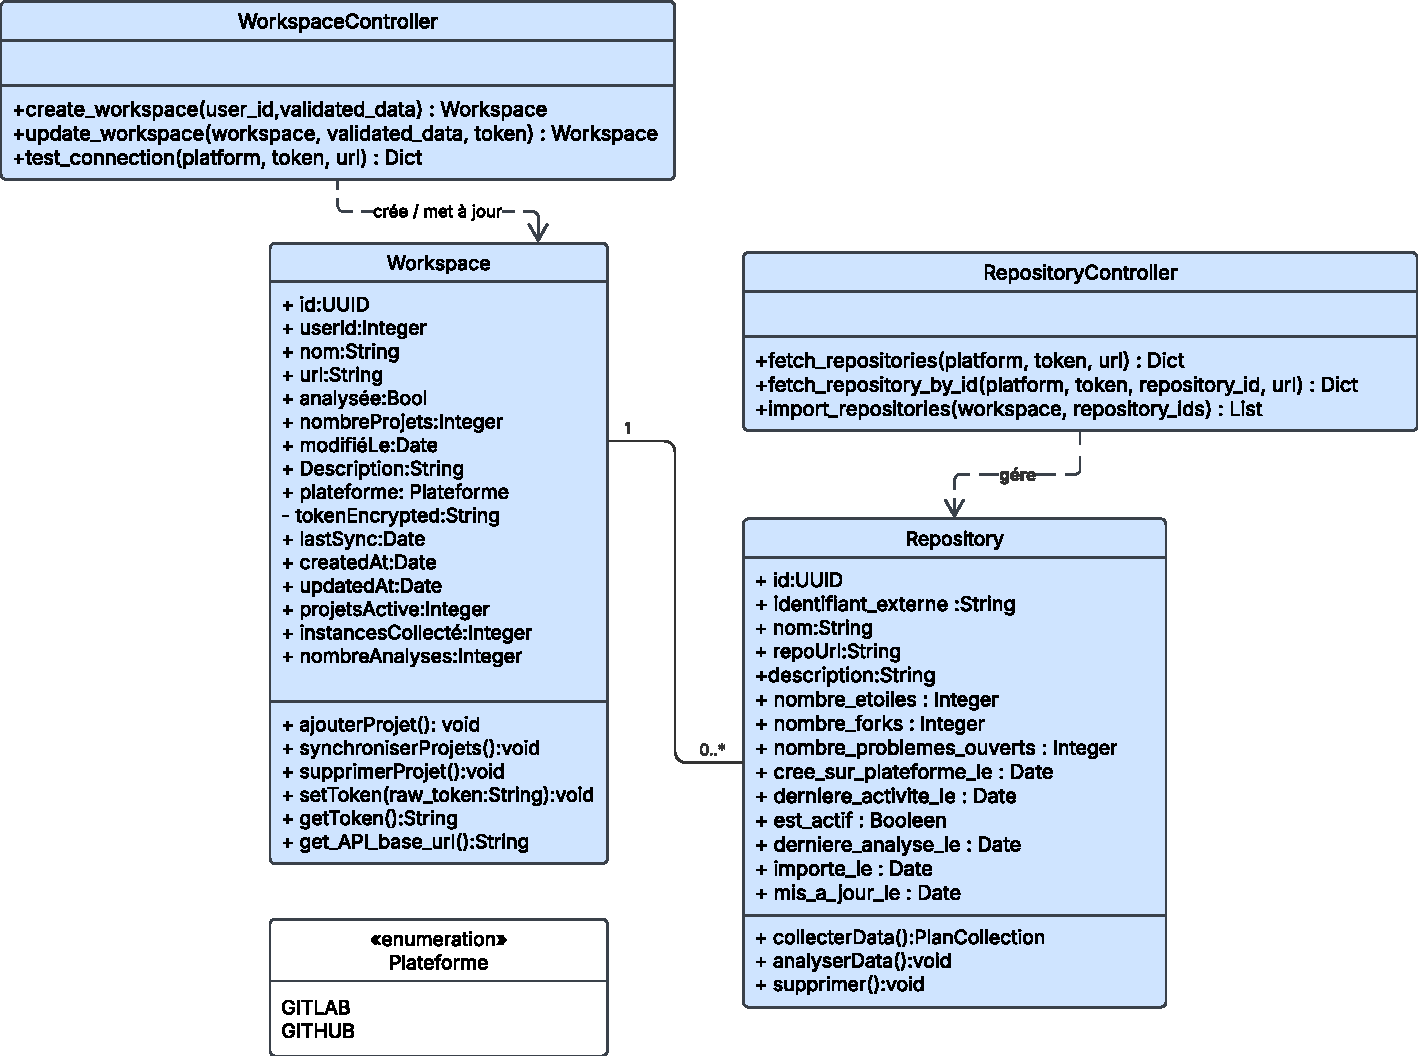
\includegraphics[width=0.9\textwidth]{classDiagramm2.pdf}
\caption{Diagramme de classes du service configuration}
\label{fig:classDiagramm2}
\end{figure}


\subsection{Service de collecte}
Le service de collecte permet d’extraire les données de revue de code à partir d’un dépôt sélectionné. La collecte peut être configurée manuellement, en précisant la branche, les endpoints, les filtres, l’état des PR/MR et la plage temporelle, ou générée automatiquement à partir d’un prompt en langage naturel.

Après validation du plan de collecte, le service extrait les données depuis GitHub ou GitLab et les stocke sous forme brute. Il permet ensuite de nettoyer et filtrer ces données afin de produire un dataset structuré, ainsi que de calculer les métriques nécessaires aux analyses futures. Il conserve également l’historique des collectes afin d’éviter les opérations répétitives.

\begin{table}[H]
\centering
\begin{tabular}{|p{4cm}|p{10cm}|}
\hline
\textbf{Élément} & \textbf{Description} \\
\hline
\textbf{Entrées} & Prompt en langage naturel ou configuration manuelle de collecte: dépôt sélectionné, branche, endpoints, filtres, plage temporelle, état des PR/MR. \\
\hline
\textbf{Sorties} & Données brutes collectées, datasets nettoyés et filtrés, fichiers structurés, métriques calculées, historique des collectes. \\
\hline
\textbf{Besoins couverts} & BF6, BF8, BF9, BF10, BF11, BF12, BF13, BF14, BF20, BF22, BF23 \\
\hline
\end{tabular}
\end{table}

\subsubsection*{Endpoints considérés pour la collecte}

Afin de permettre une analyse riche et extensible, le service de collecte est conçu pour prendre en charge différentes familles d’endpoints issues des plateformes GitHub et GitLab. L’objectif est de permettre à l’utilisateur de sélectionner les données pertinentes selon son besoin, tout en conservant la possibilité d’étendre progressivement les métriques calculées.Les principales catégories d’endpoints ciblées sont :
\begin{itemize}    
\item \textbf{Données de revue de code :} pull requests, merge requests, reviewers, auteurs, états, dates de création, fusion et fermeture.    
\item \textbf{Commentaires et discussions :} commentaires généraux, commentaires de revue, discussions et remarques associées aux PR/MR.    
\item \textbf{Commits et changements de code :} commits associés, auteurs, messages, fichiers modifiés, diffs et informations de modification.    
\item \textbf{Métadonnées de projet :} branches, labels, milestones, participants et informations générales du dépôt.    
\item \textbf{Données Kanban :} issues, boards, colonnes, statuts et informations liées au suivi du travail.    
\item \textbf{Données CI/CD :} pipelines, jobs, statuts d’exécution, durées et résultats associés.
\end{itemize}
Cette organisation par familles d’endpoints permet d’adapter la collecte aux objectifs d’analyse, tout en préparant le système à l’ajout de nouvelles métriques ou de nouvelles sources de données.

\subsubsection*{Diagramme de classes du service de collecte}

Ce diagramme présente les classes liées à la configuration, l’exécution, le nettoyage et le suivi des collectes.
\begin{figure}[H]
\centering
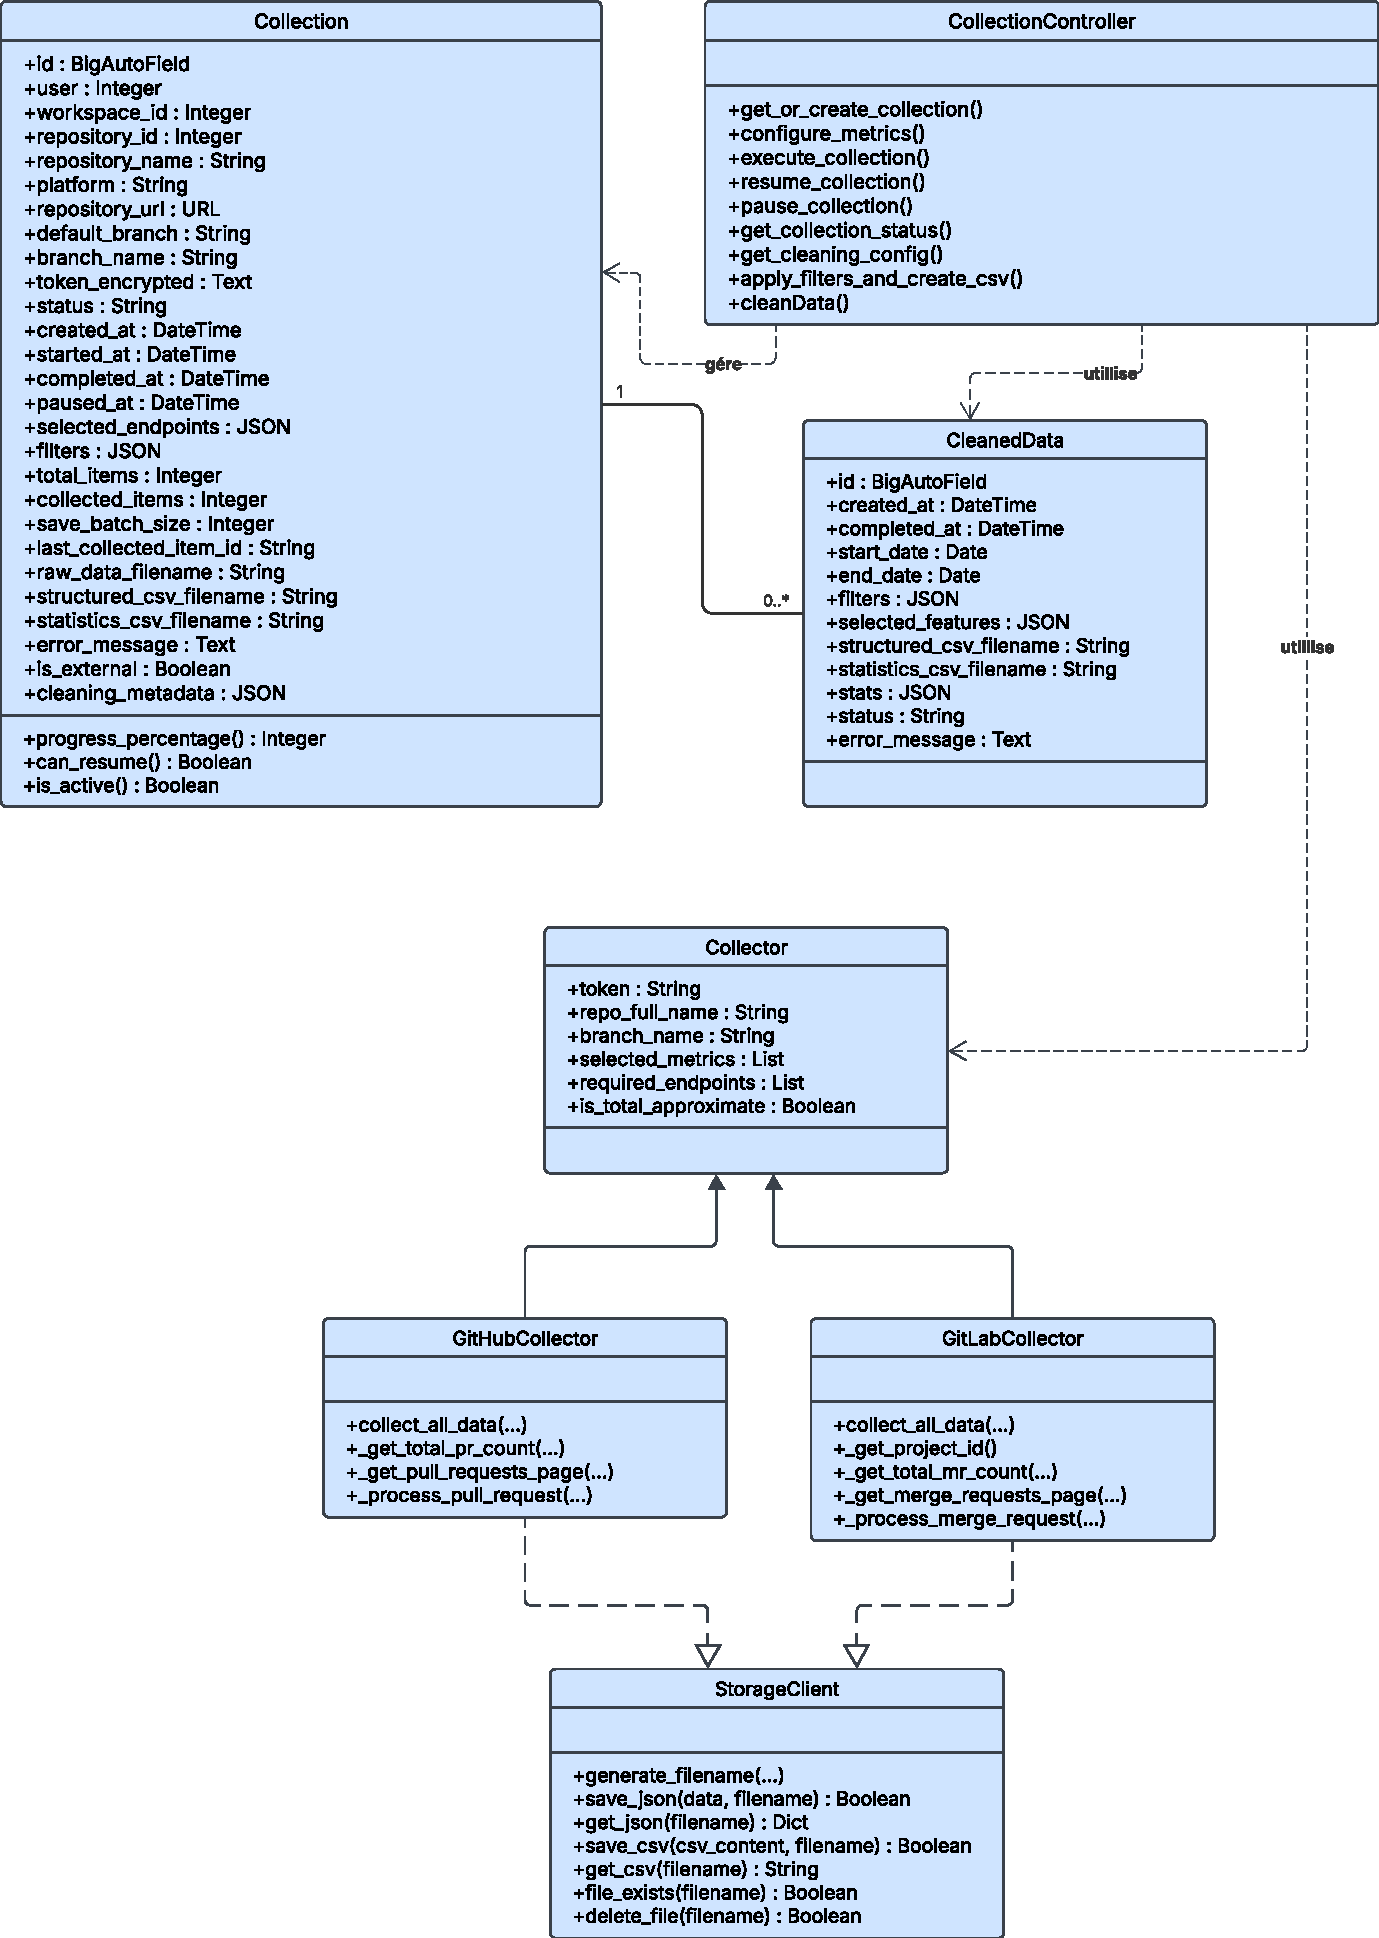
\includegraphics[width=0.9\textwidth]{classDiagramm3.pdf}
\caption{Diagramme de classes du service collection}
\label{fig:classDiagramm3}
\end{figure}

\subsection{Service d’analyse}
Le service d’analyse exploite les données collectées et les métriques calculées afin de produire des analyses, statistiques et visualisations. Il peut travailler sur des datasets issus de la collecte interne ou sur des datasets externes importés par l’utilisateur.

L’analyse peut être configurée manuellement, à partir d’analyses prédéfinies, ou automatiquement à partir d’un prompt. Les résultats sont ensuite présentés dans un tableau de bord et peuvent être exportés ou consultés depuis l’historique.

\begin{table}[H]
\centering
\begin{tabular}{|p{4cm}|p{10cm}|}
\hline
\textbf{Élément} & \textbf{Description} \\
\hline
\textbf{Entrées} & Dataset interne ou externe, métriques calculées, configuration manuelle d’analyse ou prompt utilisateur. \\
\hline
\textbf{Sorties} & Analyses, statistiques, visualisations, résultats exploitables, historique des analyses, exports. \\
\hline
\textbf{Besoins couverts} & BF13, BF16, BF17, BF18, BF19, BF20 \\
\hline
\end{tabular}
\end{table}


\subsubsection*{Diagramme de classes du service d’analyse}

Ce diagramme présente les classes liées aux datasets, aux analyses, aux résultats et aux lots d’analyse.
\begin{figure}[H]
\centering
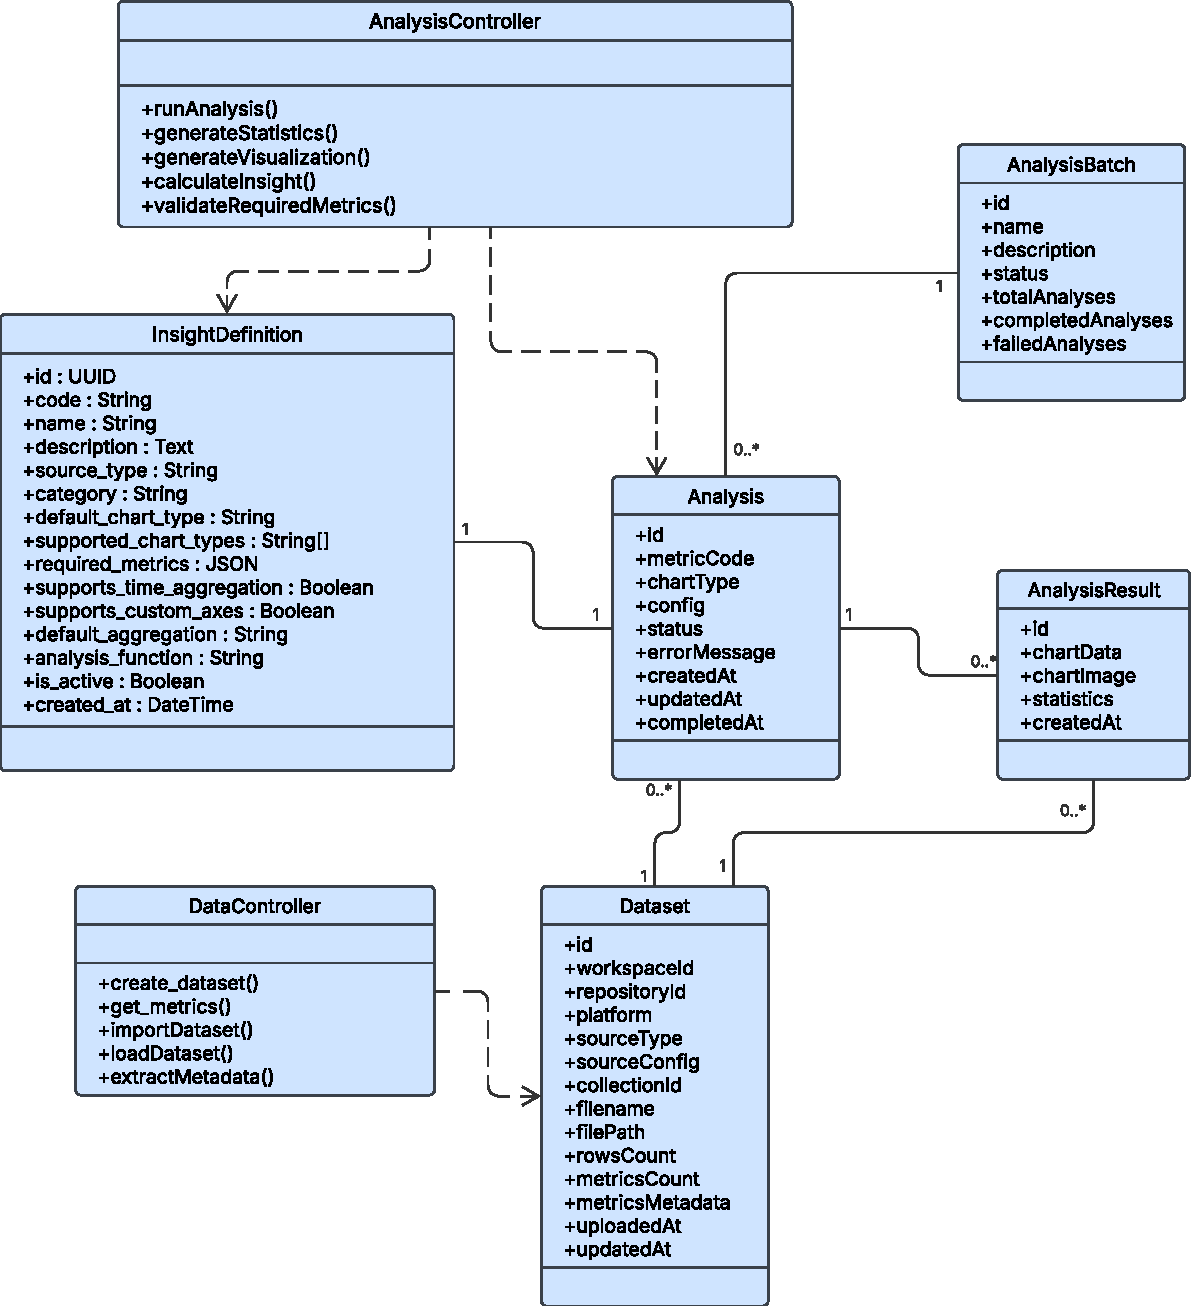
\includegraphics[width=0.9\textwidth]{classDiagramm4.pdf}
\caption{Diagramme de classes du service analyse}
\label{fig:classDiagramm4}
\end{figure}


\subsection{Service LLM}
Le service LLM permet d’intégrer l’interaction en langage naturel dans RevMine. Il interprète les prompts utilisateur afin de générer des configurations exploitables par les services de collecte ou d’analyse.

Selon le type de requête, il peut produire un plan de collecte, proposer des filtres de nettoyage, suggérer des métriques à calculer ou générer une configuration d’analyse. Il permet aussi de gérer le choix entre un modèle local ou un fournisseur externe.

\begin{table}[H]
\centering
\begin{tabular}{|p{4cm}|p{10cm}|}
\hline
\textbf{Élément} & \textbf{Description} \\
\hline
\textbf{Entrées} & Prompt utilisateur, type de requête, contexte disponible, choix du fournisseur LLM. \\
\hline
\textbf{Sorties} & Plan de collecte, configuration de nettoyage, liste de métriques à calculer, configuration d’analyse ou liste d’analyses proposées. \\
\hline
\textbf{Besoins couverts} & BF7, BF15 \\
\hline
\end{tabular}
\end{table}


\subsubsection*{Diagramme de classes du service LLM}

Ce diagramme présente les objets de requête/réponse et le fournisseur LLM utilisé.
\begin{figure}[H]
\centering
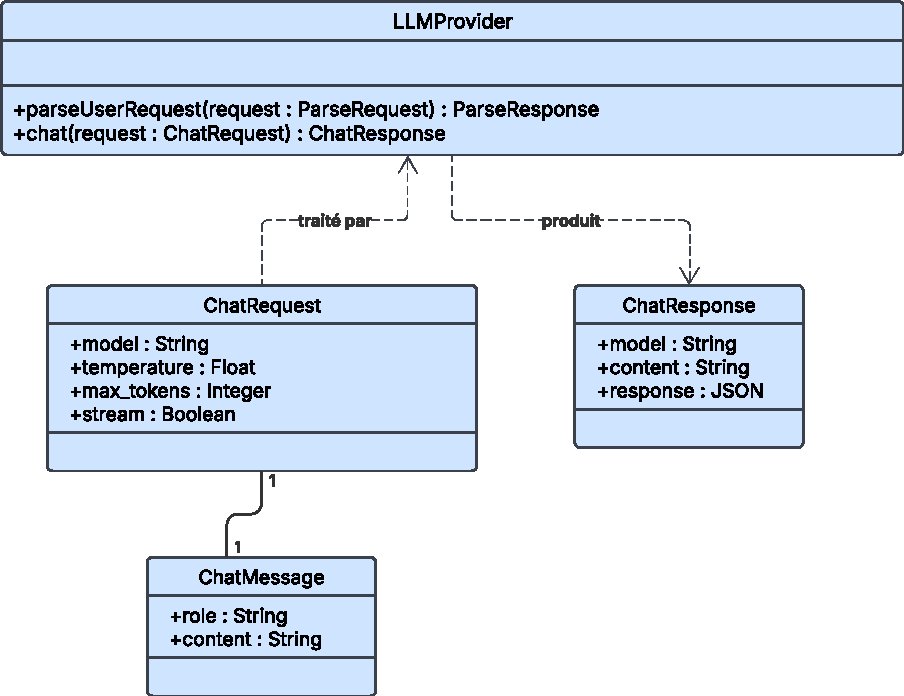
\includegraphics[width=0.9\textwidth]{classDiagramm5.pdf}
\caption{Diagramme de classes du service LLM}
\label{fig:classDiagramm5}
\end{figure}


\subsection{Service de notification}

Le service de notification informe l’utilisateur de l’état des opérations importantes de la plateforme. Il intervient notamment lors des collectes, nettoyages, calculs de métriques, analyses ou générations de plans.

Il permet de signaler le démarrage, la progression, la suspension, la reprise, la réussite ou l’échec d’une opération, améliorant ainsi le suivi et l’expérience utilisateur.

\begin{table}[H]
\centering
\begin{tabular}{|p{4cm}|p{10cm}|}
\hline
\textbf{Élément} & \textbf{Description} \\
\hline
\textbf{Entrées} & Événements produits par les services, états d’avancement, erreurs, messages système. \\
\hline
\textbf{Sorties} & Notifications utilisateur et messages de suivi. \\
\hline
\textbf{Besoins couverts} & BF21 \\
\hline
\end{tabular}
\end{table}

\subsubsection*{Diagramme de classes du service de notification}

Ce diagramme présente les classes responsables de la création, de la persistance et de la diffusion des notifications.
\begin{figure}[H]
\centering
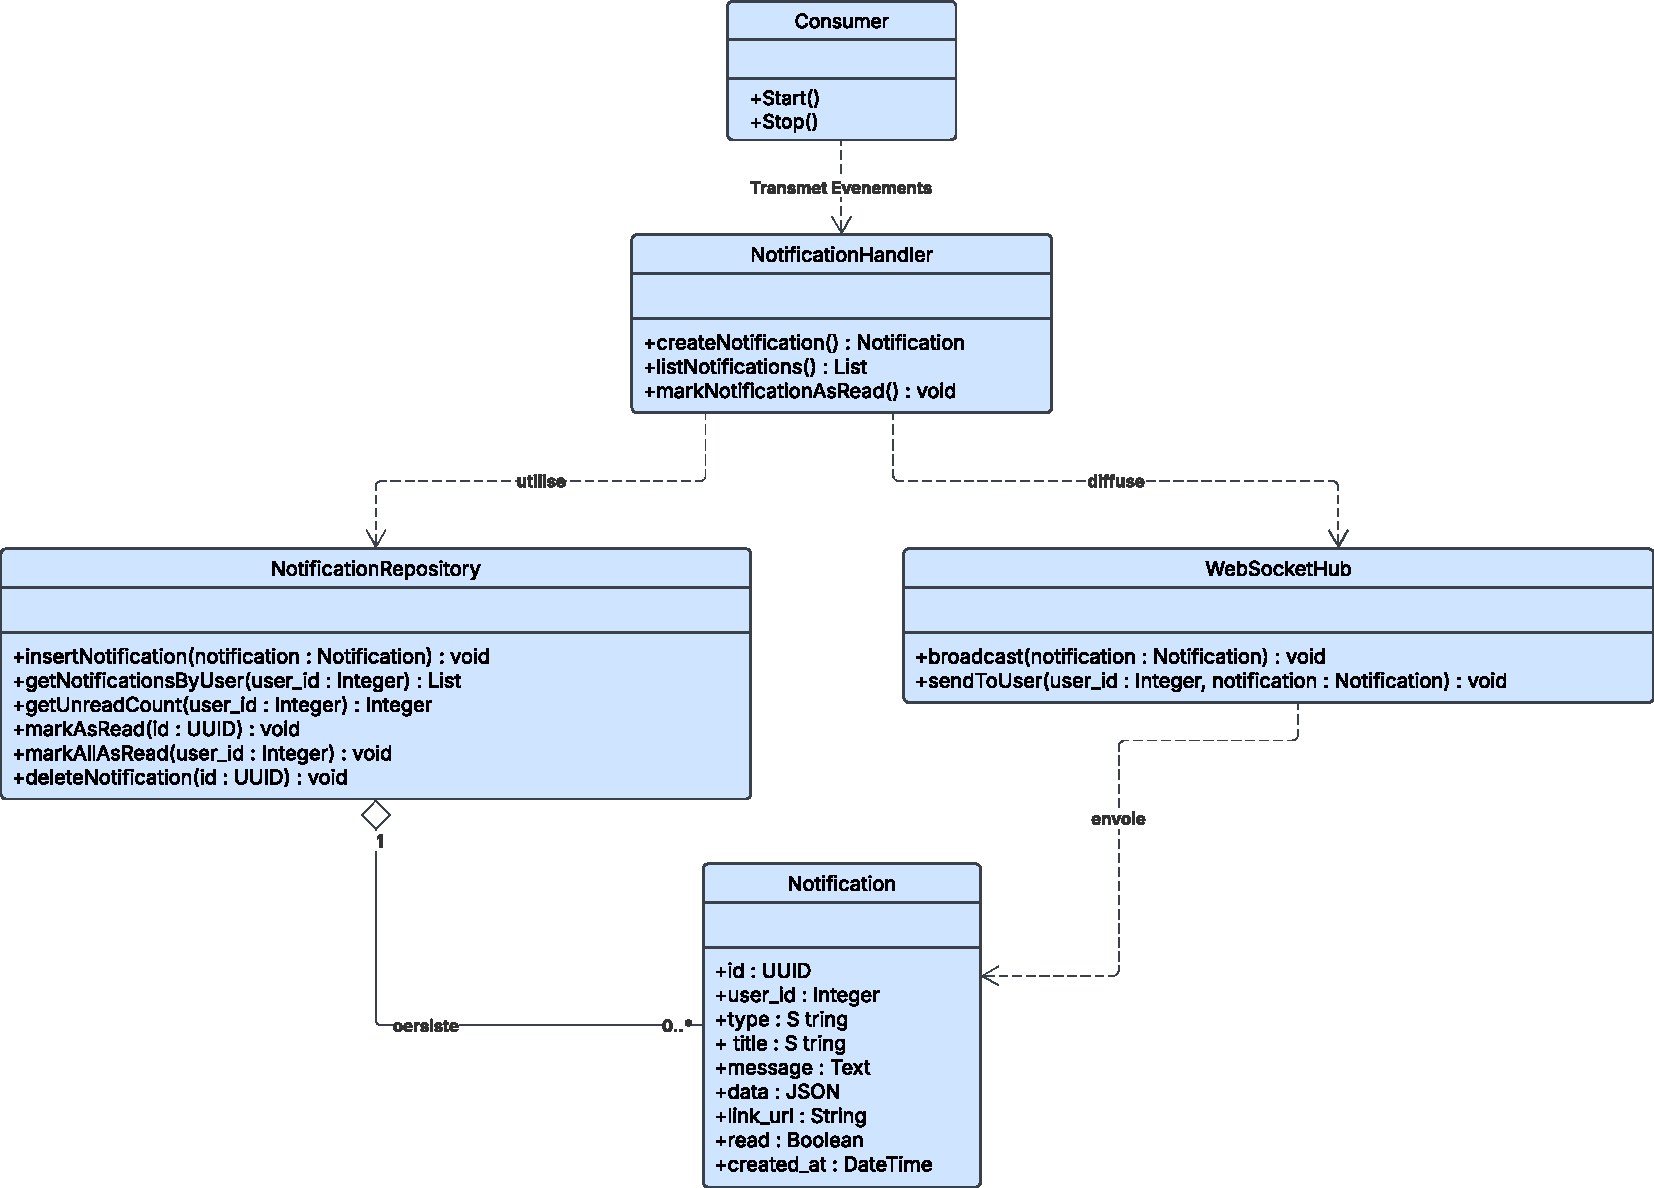
\includegraphics[width=0.9\textwidth]{classDiagramm6.pdf}
\caption{Diagramme de classes du service notification}
\label{fig:classDiagramm6}
\end{figure}


\section{Diagramme de composants global}
La figure ci-dessous synthétise la vue logique globale de RevMine en regroupant les composants détaillés précédemment. Elle permet de visualiser les principales interactions entre l’interface utilisateur, l’API Gateway, les services applicatifs, leurs espaces de persistance et les systèmes externes.

\begin{figure}[H]
    \centering
    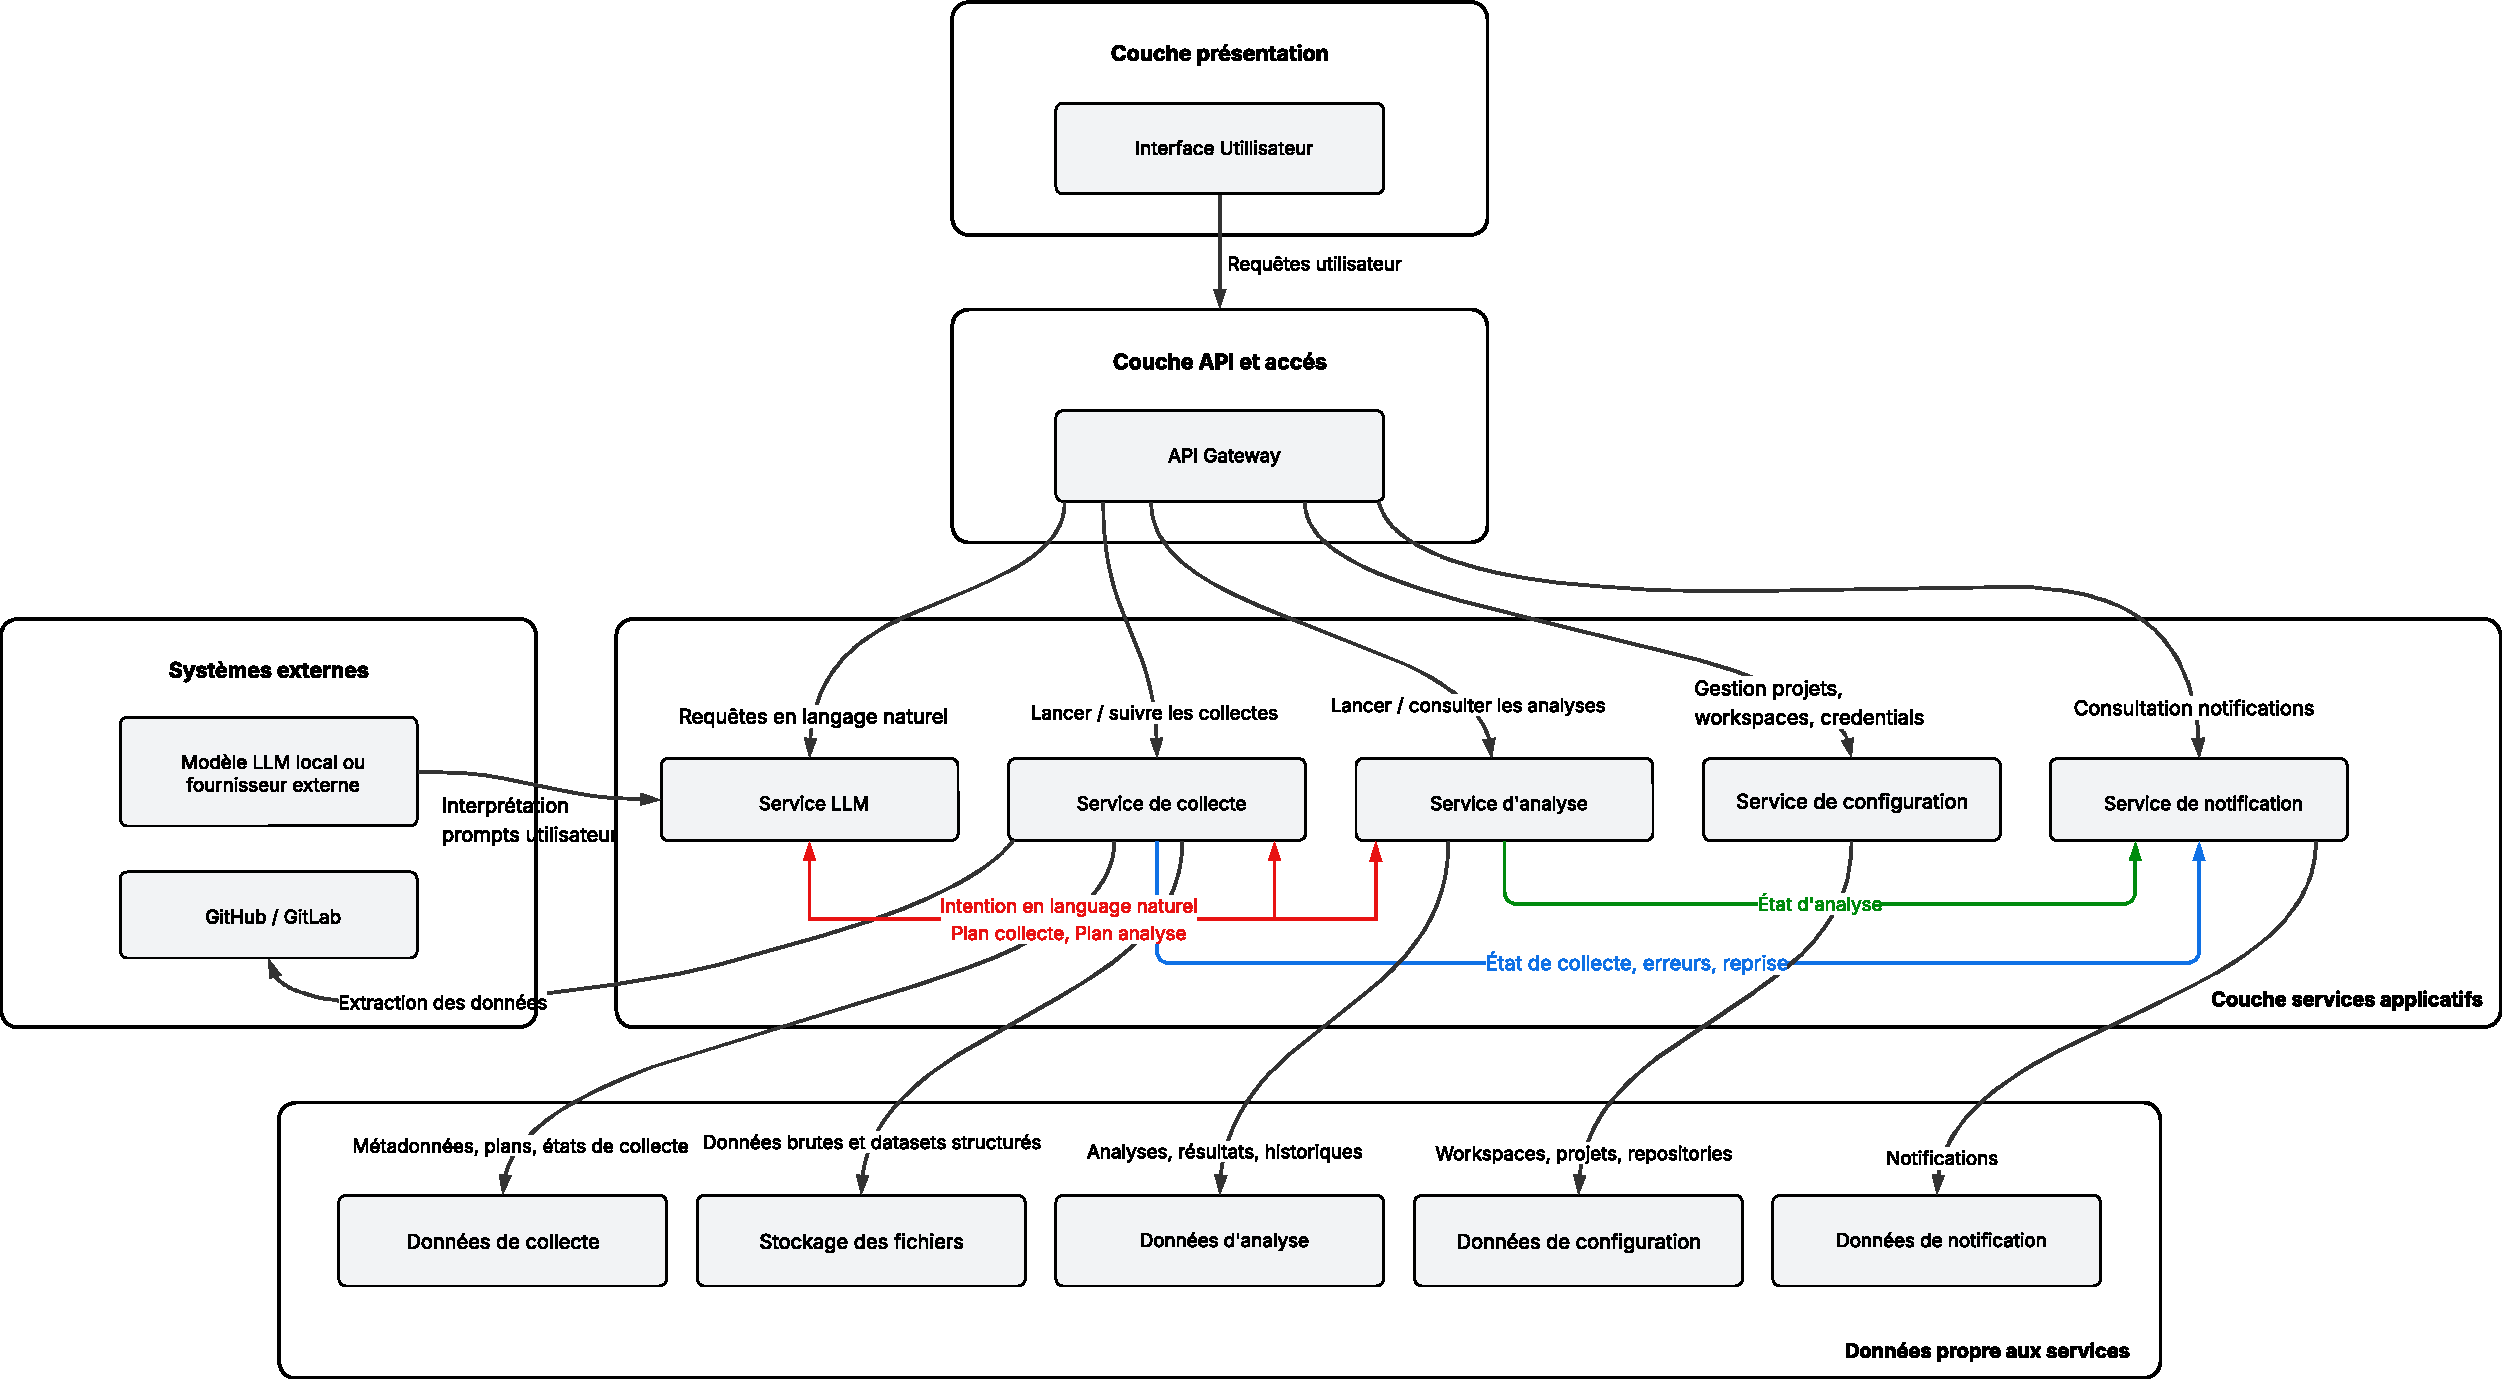
\includegraphics[width=\textwidth]{figures/diagrammComposants.pdf}
    \caption{Vue logique globale des composants de RevMine}
    \label{fig:vue-logique-composants-revmine}
\end{figure}

\section{Conclusion}
Ce chapitre a présenté la conception de la solution RevMine en partant des objectifs définis et des besoins identifiés précédemment. Après une étude comparative des principaux styles architecturaux, nous avons retenu une architecture microservices organisée en couches, adaptée à la séparation des responsabilités, à l’évolutivité et à la maintenabilité de la plateforme.

Nous avons ensuite détaillé la structure globale de RevMine ainsi que la conception interne de ses principaux services, notamment l’API Gateway, le service de configuration, le service de collecte, le service d’analyse, le service LLM et le service de notification.

Ainsi, cette phase de conception établit une base claire pour la mise en œuvre de RevMine, en traduisant les besoins fonctionnels et les choix architecturaux en une structure logicielle cohérente. Le chapitre suivant sera consacré à la réalisation de la solution, où nous présenterons les aspects d’implémentation, les technologies utilisées ainsi que les principales fonctionnalités développées.

\chapter{Réalisation}
% ============================================================
% Chapitre 6 : Réalisation, Tests et Déploiement
% ============================================================

\section{Introduction}

À l'issue des phases d'analyse des besoins et de conception architecturale, ce chapitre décrit
la concrétisation technique de la plateforme \textbf{RevMine}. Il couvre l'ensemble du processus
de réalisation~: de la mise en place de la culture DevOps et de l'environnement de développement
jusqu'à l'implémentation des différents modules du système, en passant par la stratégie de test,
le déploiement et la surveillance de la plateforme.

L'objectif de cette phase est de produire une application capable de centraliser la configuration
des espaces de travail, de collecter les données issues des plateformes de gestion de code, de les
nettoyer et de les structurer, puis de générer des analyses visuelles exploitables. Pour répondre
à ces exigences, une architecture microservices a été adoptée, avec une séparation claire des
responsabilités entre l'API Gateway, les services métier, les mécanismes de communication
asynchrone et les composants d'infrastructure.

% ============================================================
\section{Environnement de développement}
% ============================================================

\subsection{Matériel}

Le développement de RevMine a été mené en binôme sur deux postes de travail locaux. Le
Tableau~\ref{tab:env-dev} récapitule leurs configurations matérielles et logicielles.

\begin{table}[H]
\centering
\small
\caption{Configurations des postes de développement}
\label{tab:env-dev}
\begin{tabular}{|>{\raggedright\arraybackslash}p{3.5cm}
                |>{\raggedright\arraybackslash}p{5cm}
                |>{\raggedright\arraybackslash}p{5cm}|}
\hline
\textbf{Caractéristique} & \textbf{Poste 1} & \textbf{Poste 2} \\
\hline
Système d'exploitation & Windows 11 Pro (64~bits) & Windows 11 Pro (64~bits) \\
\hline
Processeur & Intel Core i5 -- 10\textsuperscript{e} génération
           & Intel Core i7 -- 10\textsuperscript{e} génération \\
\hline
Carte graphique & NVIDIA GeForce GTX~1650 & -- \\
\hline
Mémoire RAM & 8~Go & 16~Go \\
\hline
Stockage & SSD 256~Go & SSD 512~Go \\
\hline
\end{tabular}
\end{table}

\subsection{Logiciels et outils}

Les principaux outils utilisés au cours du développement sont les suivants~:

\begin{itemize}
    \item \textbf{Visual Studio Code} et \textbf{PyCharm Community Edition}~: éditeurs utilisés
          respectivement pour le développement frontend/backend généraliste et pour le développement
          Python spécialisé~;
    \item \textbf{Docker Desktop}~: plateforme de conteneurisation permettant d'exécuter et
          d'orchestrer l'ensemble des services sous Windows~;
    \item \textbf{Postman}~: outil de test et de documentation des API REST~;
    \item \textbf{Git / GitLab}~: système de gestion de versions distribué, utilisé pour le
          versioning, la gestion des branches et le suivi du projet~;
    \item \textbf{pgAdmin 4}~: interface graphique d'administration des bases de données
          PostgreSQL.
\end{itemize}

% ============================================================
\section{Technologies utilisées}
% ============================================================

\subsection{Python}
\begin{wrapfigure}{r}{0.1\textwidth}
    \centering
    
\includegraphics[width=0.1\textwidth]{assets/python_logo.png}
\end{wrapfigure}

Python est un langage de programmation interprété, multiparadigme et open source, reconnu pour
sa lisibilité, sa flexibilité et la richesse de son écosystème \parencite{pythonWhatPython}. Sa
syntaxe épurée réduit le coût de maintenance des projets, tandis que ses bibliothèques spécialisées
couvrent de nombreux domaines, de l'analyse de données à l'apprentissage automatique. Dans
RevMine, Python constitue le socle du développement backend en raison de sa maturité pour
l'interaction avec les API REST, le traitement de données et l'intégration de services
d'intelligence artificielle.

\subsection{Django et Django REST Framework}
\begin{wrapfigure}{r}{0.1\textwidth}
    \centering
    
\includegraphics[width=0.1\textwidth]{assets/django_logo.png}
\end{wrapfigure}

Django est un framework web Python suivant le paradigme Modèle-Vue-Template (MVT). Il intègre
nativement un ORM\footnote{ORM (\textit{Object-Relational Mapping})~: technique de correspondance
entre les objets d'un programme et les tables d'une base de données relationnelle, permettant de
manipuler les données sans écrire de requêtes SQL.} puissant, un système d'authentification
robuste et une interface d'administration \parencite{holovaty2009django}. Son extension Django
REST Framework (DRF) facilite la conception d'API RESTful performantes et bien documentées. Dans
RevMine, Django/DRF est utilisé pour le \textbf{service d'authentification} ainsi que pour les
services métier manipulant des données persistantes, notamment les services de configuration, de
collecte et d'analyse. Ce choix est motivé par la maturité de l'ORM avec PostgreSQL, la facilité
de structuration des API REST et l'intégration de mécanismes de sécurité déjà éprouvés.

\subsection{FastAPI}
\begin{wrapfigure}{r}{0.1\textwidth}
    \centering
    
\includegraphics[width=0.1\textwidth]{assets/fastapi_logo.png}
\end{wrapfigure}

FastAPI est un framework Python moderne orienté performances, reposant sur les annotations de
type Python~3.7+ et le paradigme asynchrone (\texttt{async/await}) \parencite{ramirez2021fastapi}.
Il génère automatiquement une documentation interactive (Swagger UI, ReDoc) et assure la
validation des données via Pydantic. Dans RevMine, FastAPI est utilisé pour deux composants où la
légèreté et l'exécution asynchrone sont importantes~: \textbf{l'API Gateway}, qui joue le rôle de
proxy applicatif entre le frontend et les microservices, et le \textbf{service LLM}, qui expose une
interface REST simple vers Ollama et OpenRouter.

\subsection{Go et WebSocket}
\begin{wrapfigure}{r}{0.1\textwidth}
    \centering
    
\includegraphics[width=0.1\textwidth]{assets/go_logo.png}
\end{wrapfigure}

Go est un langage compilé et statiquement typé, développé par Google, dont la gestion native de
la concurrence via les \textit{goroutines} en fait un choix de référence pour les services à haute
concurrence et faible latence \parencite{go2012donovan}. Le service de notification de RevMine
doit gérer simultanément un grand nombre de connexions persistantes en temps réel~; Go répond à
cette contrainte en permettant le traitement de milliers de connexions concurrentes avec une
empreinte mémoire réduite. Le framework \textbf{Fiber}, inspiré d'Express.js, a été utilisé pour
simplifier le développement des API REST associées.

Le protocole \textbf{WebSocket}\footnote{WebSocket (RFC~6455)~: protocole de communication
standardisé établissant un canal bidirectionnel et persistant entre un client et un serveur sur
une connexion TCP, contrairement à HTTP qui est unidirectionnel par nature.} établit un canal de
communication bidirectionnel et persistant, permettant au service de notification de diffuser
instantanément les événements système (démarrage de collecte, fin d'analyse, erreur) aux clients
connectés, sans recourir au \textit{polling} HTTP.

\subsection{React.js}
\begin{wrapfigure}{r}{0.1\textwidth}
    \centering
    
\includegraphics[width=0.1\textwidth]{assets/react_logo.png}
\end{wrapfigure}

React.js est une bibliothèque JavaScript open source développée par Meta pour la construction
d'interfaces utilisateur interactives, reposant sur une architecture en composants réutilisables
et une gestion efficace du DOM virtuel \parencite{facebookReact2023}. Dans RevMine, React.js
assure le développement de l'interface utilisateur, permettant l'exploration interactive des
données, la configuration des collectes et la visualisation des résultats d'analyse.

\subsection{Tailwind CSS}
\begin{wrapfigure}{r}{0.1\textwidth}
    \centering
    
\includegraphics[width=0.1\textwidth]{assets/tailwind_logo.png}
\end{wrapfigure}

Tailwind CSS est un framework CSS \textit{utility-first} qui permet de construire des interfaces
modernes et responsives directement dans le balisage, sans rédiger de feuilles de style
personnalisées volumineuses \parencite{tailwindlabs2023}. Son approche par classes utilitaires
composables favorise la cohérence visuelle et s'intègre naturellement avec React.

\subsection{Docker}
\begin{wrapfigure}{r}{0.1\textwidth}
    \centering
    
\includegraphics[width=0.1\textwidth]{assets/docker_logo.png}
\end{wrapfigure}

Docker est une plateforme de conteneurisation permettant d'empaqueter une application et ses
dépendances dans un conteneur léger, portable et isolé \parencite{merkel2014docker}. Un
\textit{conteneur} est une unité d'exécution autonome qui encapsule le code, les bibliothèques
et les configurations nécessaires au fonctionnement d'un service, garantissant ainsi un
comportement identique quel que soit l'environnement d'exécution. Docker Compose étend cette
capacité en orchestrant plusieurs services applicatifs et d'infrastructure de manière
déclarative. Dans RevMine, Docker assure la conteneurisation de l'ensemble des services,
garantissant la reproductibilité des environnements entre le développement, les tests et le
déploiement.

\subsection{PostgreSQL}
\begin{wrapfigure}{r}{0.1\textwidth}
    \centering
    
\includegraphics[width=0.1\textwidth]{assets/postgresql_logo.png}
\end{wrapfigure}

PostgreSQL est un système de gestion de base de données relationnelle objet open source, reconnu
pour sa robustesse, sa conformité aux standards SQL et ses fonctionnalités avancées
\parencite{postgresql2023}. Son intégration native avec l'ORM Django facilite la persistance des
données métier. Chaque microservice de RevMine dispose de sa propre base PostgreSQL, assurant
ainsi l'isolation des données et limitant les dépendances directes entre services.

\subsection{MinIO}
\begin{wrapfigure}{r}{0.1\textwidth}
    \centering
    
\includegraphics[width=0.1\textwidth]{assets/minio_logo.png}
\end{wrapfigure}

MinIO est une solution de stockage objet haute performance compatible avec l'API Amazon S3,
conçue pour le stockage de fichiers volumineux et de données semi-structurées
\parencite{minio2023}. Dans RevMine, MinIO archive les données brutes collectées depuis GitHub et
GitLab sous forme de fichiers JSON, séparant ainsi les artefacts bruts du stockage relationnel et
facilitant leur réutilisation sans relancer les appels API.

\subsection{Apache Kafka}
\begin{wrapfigure}{r}{0.1\textwidth}
    \centering
    
\includegraphics[width=0.1\textwidth]{assets/kafka_logo.png}
\end{wrapfigure}

Apache Kafka est une plateforme distribuée de \textit{streaming} d'événements permettant la
communication asynchrone entre services via un mécanisme de publication/souscription
(\textit{publish/subscribe}) \parencite{kreps2011kafka}. Dans ce modèle, un service
\textit{producteur} publie des messages sur un \textit{topic} -- canal logique nommé --, et un ou
plusieurs services \textit{consommateurs} s'abonnent à ce topic pour traiter les messages de
manière indépendante. Son adoption dans RevMine réduit le couplage entre microservices, améliore
la scalabilité du système et permet l'exécution de traitements indépendants ou différés.

\subsection{Redis et Celery}
\begin{wrapfigure}{r}{0.1\textwidth}
    \centering
    
\includegraphics[width=0.1\textwidth]{assets/redis_logo.png}
\end{wrapfigure}

Redis est un système de stockage clé-valeur en mémoire offrant de très hautes performances pour
la mise en cache et la récupération rapide de données \parencite{carlson2013redis}. Dans RevMine,
Redis remplit deux rôles complémentaires~: le cache applicatif, qui réduit le nombre de requêtes
répétitives vers les bases de données, et le broker de messages pour Celery.

Celery est un gestionnaire de tâches asynchrones pour Python qui permet d'exécuter des
traitements longs en arrière-plan, sans bloquer la réponse aux requêtes HTTP. Cette combinaison
Redis~+~Celery améliore la réactivité globale de la plateforme, notamment lors de l'analyse de
jeux de données volumineux.

\subsection{SonarQube}
\label{subsec:sonarqube-tech}
\begin{wrapfigure}{r}{0.1\textwidth}
    \centering
    
\includegraphics[width=0.1\textwidth]{assets/sonarqube_logo.png}
\end{wrapfigure}

SonarQube est une plateforme d'analyse statique de la qualité du code, capable de détecter des
bugs, des vulnérabilités de sécurité, des \textit{code smells} et des duplications
\parencite{campbell2013sonarqube}. Dans RevMine, une configuration SonarQube Community~10.4 a été
préparée afin de permettre l'analyse statique du backend dans un environnement disposant d'un
serveur SonarQube. Cette configuration inclut les sources à analyser, les exclusions, les rapports
de couverture et les paramètres du \textit{Quality Gate}. Le pipeline GitLab CI peut ainsi être
connecté à un serveur SonarQube au moyen des variables \texttt{SONAR\_HOST\_URL} et
\texttt{SONAR\_TOKEN}. Lorsque cette étape est activée dans l'environnement CI, le
\textit{Quality Gate} peut être rendu bloquant~; dans le cadre de ce rapport, il est donc présenté
comme une capacité d'intégration qualité préparée pour l'environnement de déploiement.

\subsection{Grafana, Loki et Promtail}
\label{subsec:grafana-tech}
\begin{wrapfigure}{r}{0.1\textwidth}
    \centering
    
\includegraphics[width=0.1\textwidth]{assets/grafana_logo.png}
\end{wrapfigure}

La supervision des journaux applicatifs repose sur la pile \textbf{Loki~+~Promtail~+~Grafana}
\parencite{grafana2023loki}. Cette solution a été préférée à des alternatives plus lourdes
(ELK Stack) en raison de sa faible empreinte mémoire, de son intégration native dans un
environnement Docker et de la rapidité de sa mise en place.

\begin{itemize}
    \item \textbf{Promtail}~: agent déployé comme conteneur Docker, il collecte les journaux de
          sortie standard (\texttt{stdout}/\texttt{stderr}) de chaque conteneur applicatif et les
          expédie vers Loki~;
    \item \textbf{Loki}~: moteur de stockage et d'indexation des journaux optimisé pour les
          environnements conteneurisés. Contrairement à Elasticsearch, Loki n'indexe que les
          métadonnées (\textit{labels}), ce qui réduit considérablement la consommation de
          ressources~;
    \item \textbf{Grafana}~: interface de visualisation permettant d'interroger Loki via le
          langage de requête LogQL, d'afficher les journaux en temps réel et de configurer des
          alertes. Dans RevMine, chaque service produit ses journaux en JSON structuré,
          permettant à Grafana de filtrer rapidement les erreurs et d'identifier les anomalies
          par service, par niveau de sévérité ou par période.
\end{itemize}

% ============================================================
\section{Culture DevOps}
% ============================================================

\subsection{Principes généraux}

Le développement de RevMine s'inscrit dans une culture \textbf{DevOps}, paradigme qui rapproche
les équipes de développement (\textit{Dev}) et d'exploitation (\textit{Ops}) afin de livrer des
logiciels de manière plus rapide, plus fiable et plus itérative \parencite{bass2015devops}. DevOps
repose sur un ensemble de pratiques couvrant l'intégralité du cycle de vie du logiciel~: codage,
construction, test, déploiement et surveillance. Ce cycle est souvent représenté sous la forme
d'une boucle infinie (symbole $\infty$) illustrant la continuité et l'amélioration permanente
du processus, comme illustré à la Figure~\ref{fig:devops-cycle}.

\begin{figure}[H]
    \centering
    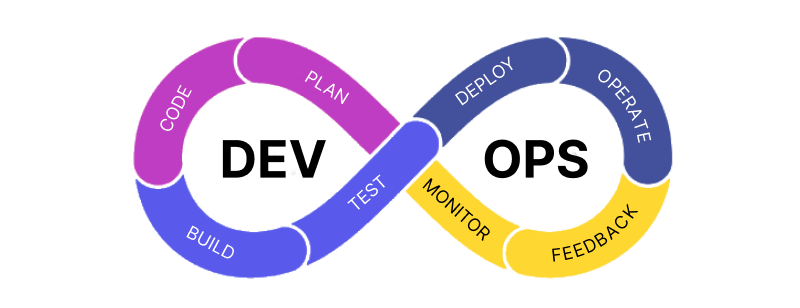
\includegraphics[width=0.75\textwidth]{assets/devops_cycle.png}
    \caption{Cycle de vie DevOps -- boucle d'amélioration continue (Source : \cite{katalon2024devops})}
    \label{fig:devops-cycle}
\end{figure}

Concrètement, les pratiques DevOps retenues pour RevMine se déclinent selon les différentes
étapes du cycle DevOps~:

\begin{itemize}
    \item \textbf{Planification (Plan)}~: définition des besoins fonctionnels et techniques du
          système, rédaction des exigences, organisation des tâches et planification des sprints
          selon la méthodologie Scrum~;

    \item \textbf{Développement (Code)}~: développement collaboratif sur GitLab avec gestion de
          versions et revue systématique des contributions via des Merge Requests~;

    \item \textbf{Construction (Build)}~: génération et construction automatisée des images Docker
          après chaque fusion sur la branche principale. Chaque service dispose de son propre
          \texttt{Dockerfile}~;

    \item \textbf{Tests (Test)}~: exécution automatique des tests unitaires, des tests
          d'intégration et des analyses de qualité statique via les pipelines GitLab CI à
          chaque commit~;

    \item \textbf{Déploiement (Deploy)}~: orchestration et déploiement des services applicatifs
          et d'infrastructure à l'aide de Docker Compose et du pipeline CI/CD GitLab~;

    \item \textbf{Exploitation (Operate)}~: gestion et exécution continue des services de la
          plateforme afin d'assurer leur disponibilité, leur stabilité et leur bon fonctionnement
          dans l'environnement de développement et de recherche~;

    \item \textbf{Retour d'expérience (Feedback)}~: collecte des retours de l'équipe de recherche
          de l'ETS ainsi que des utilisateurs métier afin d'améliorer les fonctionnalités,
          l'ergonomie et les performances du système~;

    \item \textbf{Surveillance (Monitor)}~: suivi des journaux applicatifs via la pile
          Grafana~+~Loki~+~Promtail, supervision des erreurs et observation des performances des
          services en temps réel.
\end{itemize}

Ce cycle est itératif~: les retours collectés durant les phases d'exploitation et de surveillance
permettent de revenir à l'étape de planification afin d'identifier de nouveaux besoins, corriger
les limitations observées et améliorer continuellement la plateforme RevMine.

% ============================================================
\section{Planification}
% ============================================================

\subsection{Méthodologie Scrum}

La gestion du projet s'est inspirée de la méthode \textbf{Scrum}, cadre agile structurant le
développement en itérations courtes et régulières appelées \textit{sprints}
\parencite{schwaber2020scrum}. Les sprints ont été fixés à une durée d'une semaine, permettant
des cycles de livraison rapides et une adaptation continue aux retours obtenus.

Le projet RevMine a été réalisé en \textbf{binôme}, ce qui a nécessité une coordination étroite
tout au long du développement. Deux cadences de réunion ont structuré le suivi du projet~:

\begin{itemize}
    \item \textbf{Réunions hebdomadaires (chaque jeudi)}~: ces séances servaient à la fois de
          revue de sprint et de planification. Nous y présentions les fonctionnalités développées
          au cours de la semaine, levions les blocages techniques et définissions les objectifs du
          sprint suivant. La régularité de ces rendez-vous a permis une adaptation rapide aux
          retours et un alignement continu entre les réalisations et les attentes du projet~;

    \item \textbf{Réunions mensuelles}~: à un rythme mensuel, l'équipe présentait l'avancement
          global du projet devant l'équipe de recherche de l'\textbf{ETS} (École de Technologie
          Supérieure). Ces réunions constituaient une opportunité précieuse d'obtenir un retour
          critique de la part de professionnels du métier, apportant un regard extérieur sur les
          choix fonctionnels et techniques de la plateforme. Les observations formulées lors de
          ces séances ont contribué à affiner certaines orientations du projet et à valider la
          pertinence des fonctionnalités développées au regard des besoins réels du terrain.
\end{itemize}

Cette double cadence de suivi -- hebdomadaire pour le pilotage opérationnel et mensuelle pour la
validation avec l'équipe de recherche -- a favorisé une livraison incrémentale des fonctionnalités
et une détection précoce des écarts tout au long du développement.

\subsection{Tableau Kanban}

La gestion des tâches a été assurée à l'aide du tableau \textbf{Kanban} (littéralement
\og{}panneau visuel\fg{} en japonais) intégré à GitLab. Cet outil offre une représentation
visuelle de l'état d'avancement de chaque tâche, permettant aux deux membres du binôme
d'identifier rapidement les blocages et de prioriser les efforts. Chaque fonctionnalité,
correction ou amélioration a été formalisée sous forme d'\textit{issue}, puis suivie tout au
long de son cycle de vie grâce à cinq statuts distincts et un système d'étiquettes structuré.

\subsubsection*{Statuts du tableau}

Cinq statuts ont été définis pour refléter fidèlement l'avancement de chaque tâche~:

\begin{itemize}
    \item \textbf{À faire} (\textit{To Do})~: la tâche est identifiée et planifiée pour le sprint
          en cours, mais le développement n'a pas encore débuté~;
    \item \textbf{En cours} (\textit{In Progress})~: le développement est actif~; une seule
          personne du binôme est responsable de la tâche à ce stade afin d'éviter les conflits
          de travail~;
    \item \textbf{En revue} (\textit{Under Review})~: le développement est terminé et une Merge
          Request a été ouverte~; la tâche est en attente de revue par l'autre membre du binôme
          avant intégration~;
    \item \textbf{Bloquée} (\textit{Blocked})~: la tâche ne peut pas avancer en raison d'une
          dépendance non résolue ou d'un blocage technique~; ce statut permet de signaler
          rapidement les obstacles et de les traiter en priorité lors des points hebdomadaires~;
    \item \textbf{Clôturée} (\textit{Closed})~: la tâche est terminée, revue, intégrée dans la
          branche principale et validée.
\end{itemize}

\subsubsection*{Système d'étiquettes}

Chaque issue est enrichie d'un ensemble d'étiquettes permettant de la caractériser selon plusieurs
dimensions~:

\begin{itemize}
    \item \textbf{Composant}~: \texttt{frontend}, \texttt{backend} ou \texttt{ai}, indiquant la
          couche technique concernée~;
    \item \textbf{Nature}~: \texttt{feat} (nouvelle fonctionnalité) ou \texttt{bug} (correction
          d'un défaut)~;
    \item \textbf{Priorité}~: niveau d'urgence parmi \texttt{low}, \texttt{medium} et
          \texttt{high}, facilitant l'arbitrage lors de la planification du sprint~;
    \item \textbf{Sprint}~: étiquette indiquant le sprint auquel la tâche est rattachée, assurant
          la traçabilité de la charge de travail par itération.
\end{itemize}

La Figure~\ref{fig:kanban} illustre le tableau Kanban tel qu'utilisé dans GitLab, avec les
différentes colonnes de statut et le système d'étiquettes.

\begin{figure}[H]
    \centering
    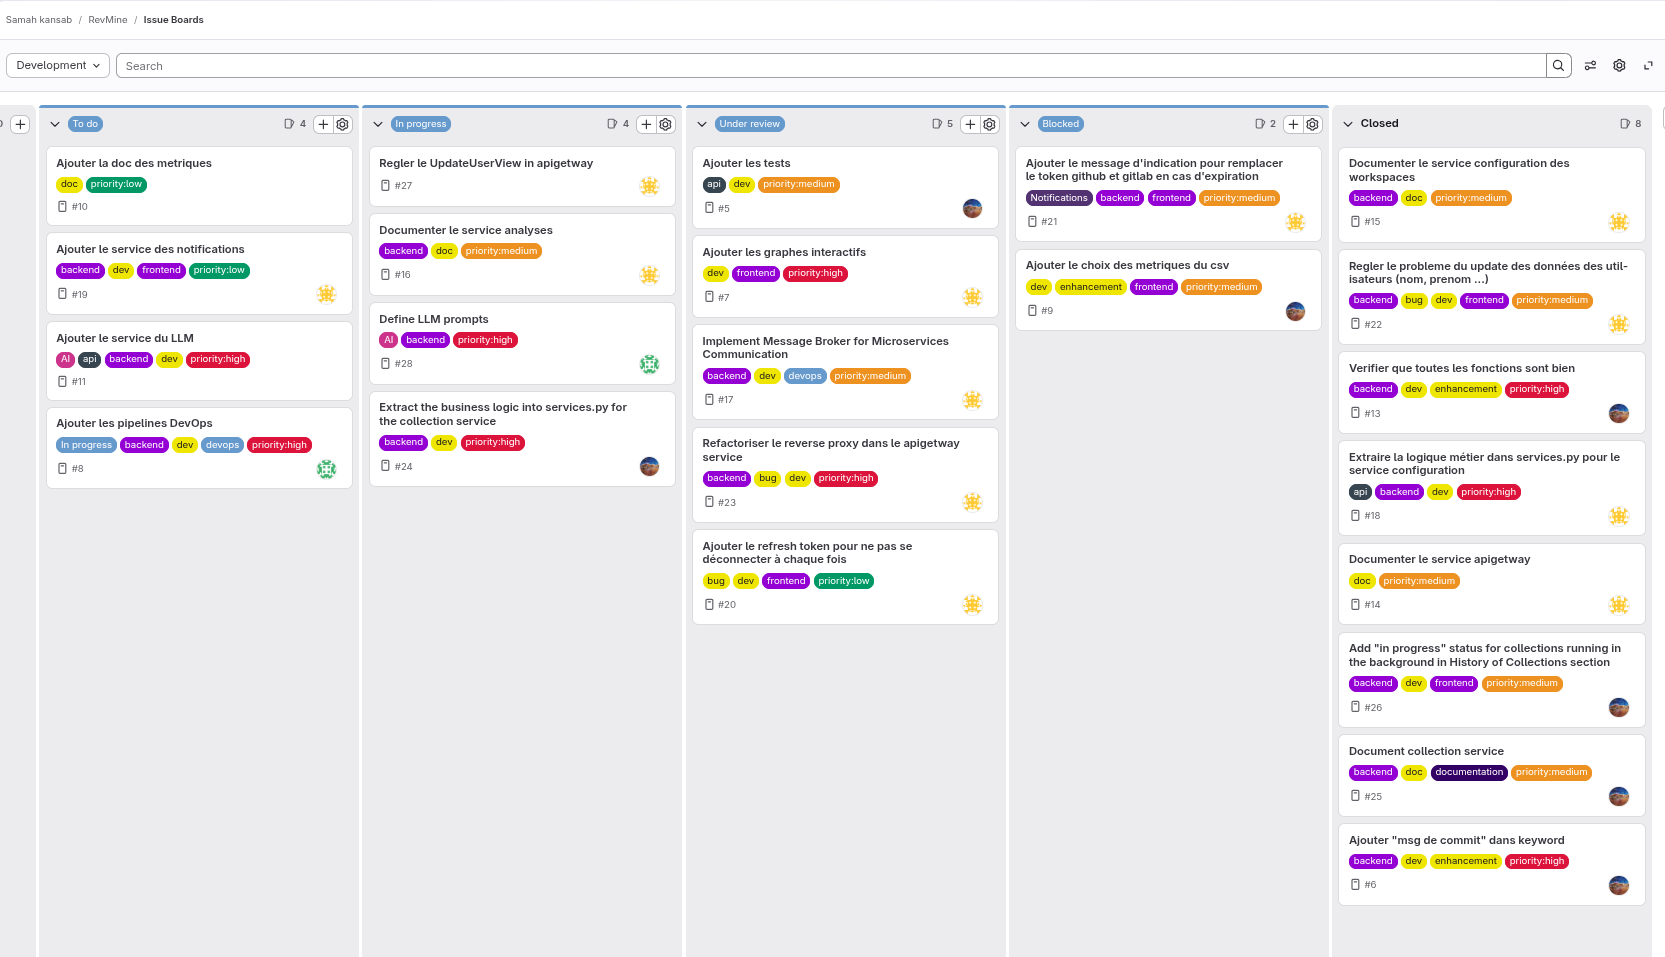
\includegraphics[width=0.95\textwidth]{captures/kanban_board.png}
    \caption{Tableau Kanban GitLab utilisé pour le suivi des tâches du projet RevMine}
    \label{fig:kanban}
\end{figure}


% ============================================================
\section{Développement}
% ============================================================

\subsection{Politique de gestion des branches}

Afin de maintenir la lisibilité de l'historique Git et de sécuriser l'intégrité de la branche
principale, une \textbf{politique de branches} rigoureuse a été adoptée, s'inspirant du
\textit{Feature Branch Workflow} \parencite{atlassian2023gitflow}. Ce modèle préconise que chaque
nouvelle unité de travail -- fonctionnalité, correction ou amélioration -- soit développée dans
une branche dédiée, isolant ainsi les modifications en cours des livrables stables.

\subsubsection*{Justification du choix}

Plusieurs alternatives ont été envisagées. Le modèle \textit{Gitflow} classique, avec ses branches
\texttt{develop}, \texttt{release} et \texttt{hotfix}, s'avère surdimensionné pour un binôme
réalisant des livraisons continues sans gestion de versions numérotées. Le \textit{Trunk-Based
Development}, où tous les développeurs poussent directement sur la branche principale, présente un
risque élevé d'instabilité pour un projet en construction active. Le \textit{Feature Branch
Workflow} représente le meilleur compromis~: chaque fonctionnalité est isolée dans sa propre
branche, ce qui protège la branche principale tout en restant simple à opérer à deux.

\subsubsection*{Convention de nommage}

La convention de nommage suivante a été appliquée de manière systématique~:

\begin{itemize}
    \item \texttt{feature/<nom-fonctionnalité>}~-- développement d'une nouvelle fonctionnalité~;
    \item \texttt{fix/<description-du-bug>}~-- correction d'un défaut~;
    \item \texttt{refactor/<module>}~-- refactorisation d'un composant existant~;
    \item \texttt{test/<service>}~-- ajout ou mise à jour de tests~;
    \item \texttt{docs/<sujet>}~-- modification de la documentation.
\end{itemize}

Ce nommage structuré présente plusieurs avantages~: il permet d'identifier instantanément la
nature et la portée d'une branche, facilite le filtrage et la recherche dans l'historique Git,
et réduit les risques de confusion lors des revues de code. Toutes les branches sont créées
depuis \texttt{main} et fusionnées après revue via une Merge Request. Aucun commit direct sur
la branche principale n'est autorisé, garantissant ainsi la stabilité permanente du code de
référence.

\subsection{Revue de code}

La branche \texttt{main} du dépôt GitLab a été configurée en mode \textbf{protégé}~: aucun
commit direct n'y est autorisé, et toute intégration passe obligatoirement par une
\textbf{Merge Request} (MR). Ce mécanisme constitue le point de contrôle central de la qualité
du code tout au long du développement.

Selon la nature et la portée de la tâche, deux niveaux de revue ont été appliqués~:

\begin{itemize}
    \item \textbf{Revue croisée}~: pour les fonctionnalités significatives, les modifications
          d'architecture ou les corrections de bugs critiques, la MR est soumise à l'examen de
          l'autre membre du binôme et, lorsque pertinent, à l'encadrant. La revue porte sur la
          correction fonctionnelle, la lisibilité du code, le respect des conventions de nommage
          et de structure, ainsi que l'absence de régressions. Les remarques sont formulées
          directement sous forme de commentaires inline dans GitLab, favorisant un échange précis
          et traçable~;
    \item \textbf{Auto-approbation}~: pour les tâches mineures -- corrections typographiques dans
          la documentation, ajustements de configuration, mises à jour de dépendances sans impact
          fonctionnel -- le membre ayant ouvert la MR procède lui-même à son approbation
          (\textit{self-approve}), afin de ne pas bloquer inutilement le flux de travail sur des
          changements à faible risque.
\end{itemize}

Cette politique à deux vitesses permet de concilier rigueur et agilité~: les modifications
sensibles bénéficient d'un regard extérieur systématique, tandis que les tâches routinières ne
génèrent pas de délais d'attente superflus. La Figure~\ref{fig:code-review} illustre un exemple
de revue de code réalisée sur une Merge Request, avec des commentaires formulés directement sur
les lignes concernées.

\begin{figure}[H]
    \centering
    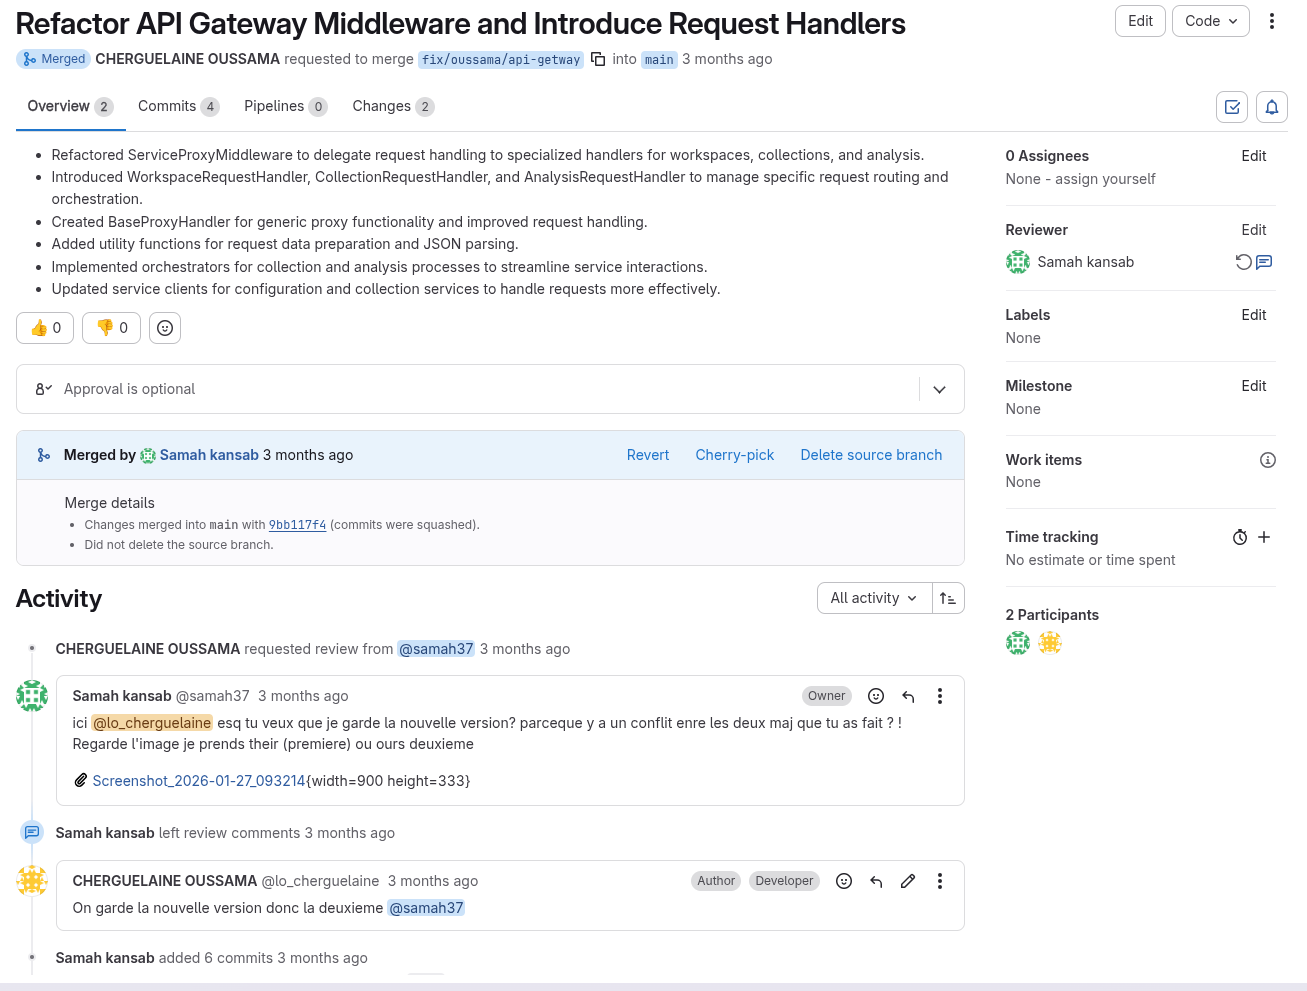
\includegraphics[width=0.95\textwidth]{captures/code_review.png}
    \caption{Exemple de revue de code sur une Merge Request GitLab dans le projet RevMine}
    \label{fig:code-review}
\end{figure}

\subsection{Réalisation du backend}

Le backend de RevMine est composé de plusieurs microservices spécialisés, chacun prenant en
charge un périmètre fonctionnel précis. Les sections suivantes détaillent l'implémentation de
chacun d'eux.

La Figure~\ref{fig:architecture-revmine-realisation} présente la vue d'ensemble de la plateforme
telle qu'elle a été réalisée. Elle distingue les services applicatifs, les bases de données
isolées, le stockage objet MinIO, le bus Kafka, le couple Redis/Celery, la pile d'observabilité
et les intégrations externes.

\begin{figure}[H]
    \centering
    \IfFileExists{assets/architecture_vf.pdf}{%
        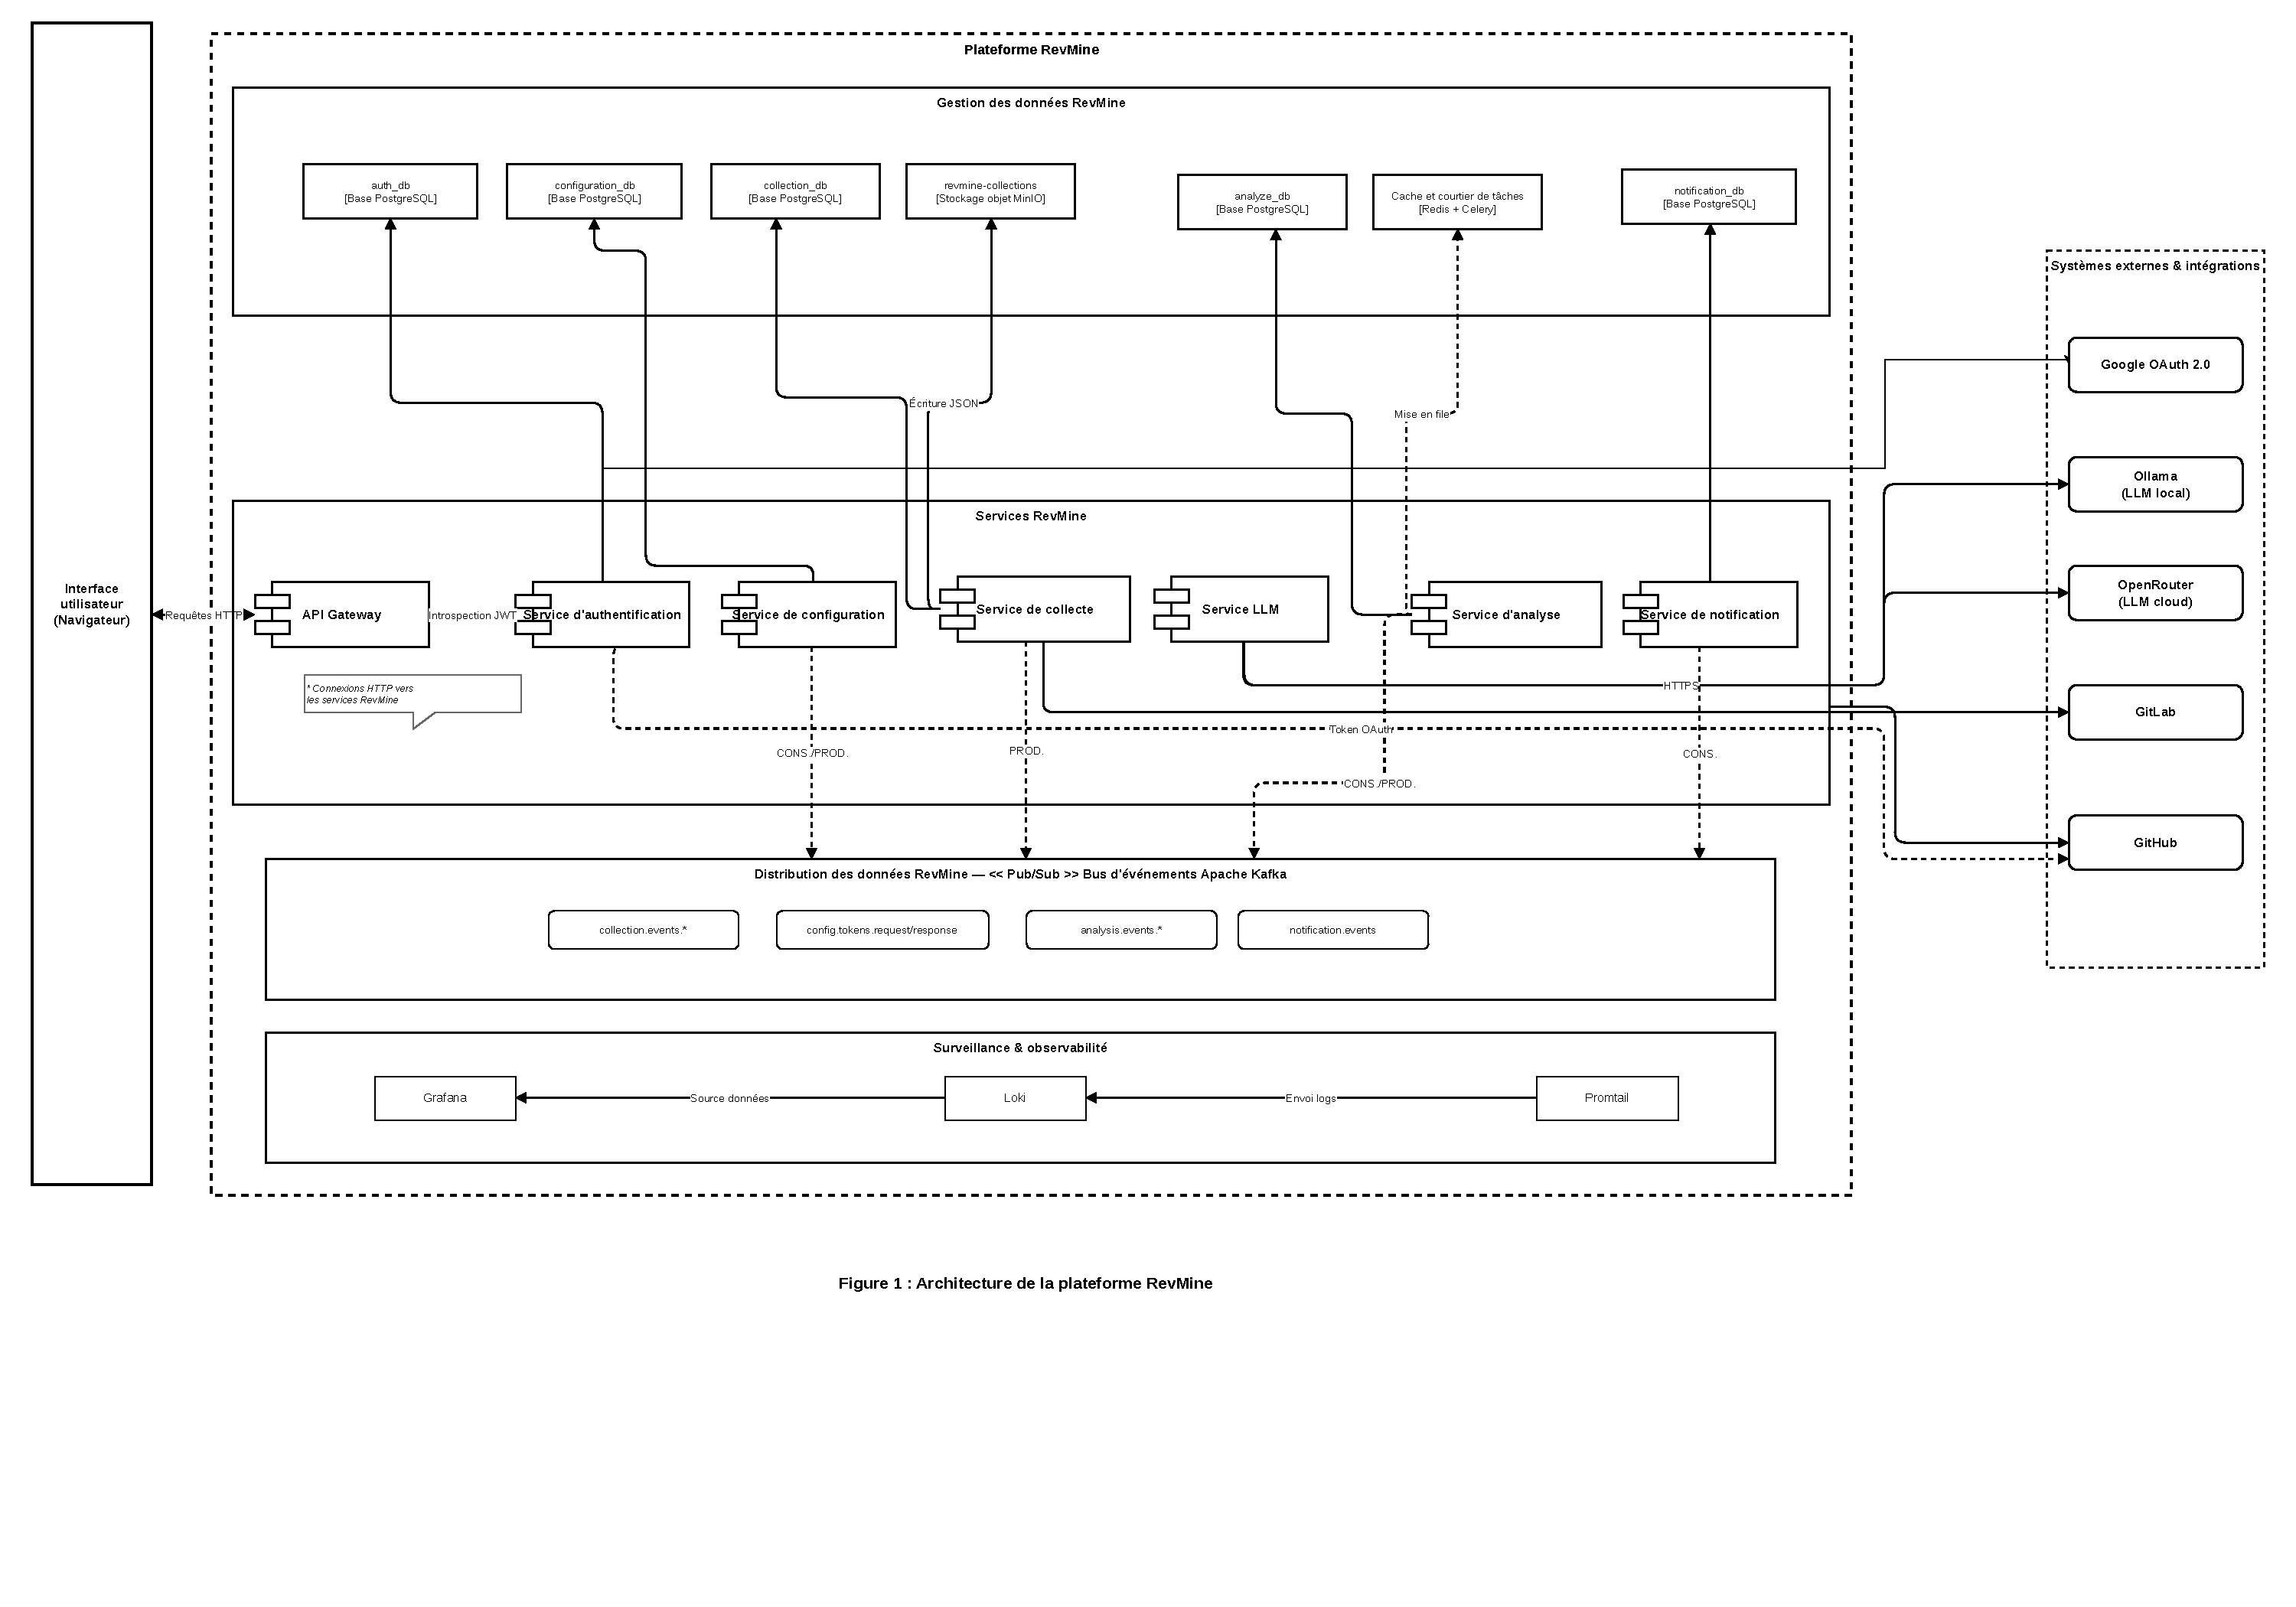
\includegraphics[
            width=\textwidth,
            height=0.68\textheight
        ]{assets/architecture_vf.pdf}%
    }{%
        \fbox{\parbox{0.9\textwidth}{\centering Diagramme d'architecture à placer dans \texttt{assets/architecture\_vf.pdf}}}%
    }
    \caption{Architecture réalisée de la plateforme RevMine}
    \label{fig:architecture-revmine-realisation}
\end{figure}

% ------------------------------------------------------------
\subsubsection{API Gateway}
% ------------------------------------------------------------

L'API Gateway constitue le point d'entrée API de RevMine. Ce composant
est développé avec \textbf{FastAPI} et agit comme un proxy applicatif léger entre le frontend et
les microservices internes. Son rôle principal est de router les requêtes,
d'appliquer les règles transversales et de propager l'identité de l'utilisateur vers les services
métier.

Son fonctionnement repose sur les responsabilités suivantes~:
\begin{itemize}
    \item réception de toutes les requêtes HTTP exposées sous le préfixe \texttt{/api/}~;
    \item routage vers le service cible selon le préfixe demandé~: authentification,
          configuration, collecte, analyse, LLM ou notification~;
    \item validation des requêtes protégées par introspection du JWT auprès du service
          d'authentification~;
    \item ajout de l'en-tête interne \texttt{X-User-ID} avant transmission au microservice cible~;
    \item gestion du CORS, des erreurs de disponibilité et d'un mécanisme de limitation de débit
          afin de réduire les abus côté client.
\end{itemize}

Le Tableau~\ref{tab:endpoints-gateway} synthétise les principales familles de routes routées par
l'API Gateway.

\begin{table}[H]
\centering
\small
\caption{Familles de routes prises en charge par l'API Gateway}
\label{tab:endpoints-gateway}
\renewcommand{\arraystretch}{1.15}
\begin{tabular}{|>{\raggedright\arraybackslash}p{4cm}
                |>{\raggedright\arraybackslash}p{4.2cm}
                |>{\raggedright\arraybackslash}p{5cm}|}
\hline
\textbf{Préfixe exposé} & \textbf{Service cible} & \textbf{Rôle} \\
\hline
\texttt{/health} & API Gateway & Vérification de disponibilité du point d'entrée \\
\hline
\texttt{/api/auth/*} & Service d'authentification & Inscription, connexion, profil, OAuth et introspection JWT \\
\hline
\texttt{/api/workspaces/*} & Service de configuration & Workspaces, plateformes, tokens chiffrés et dépôts importés \\
\hline
\texttt{/api/collections/*} & Service de collecte & Plans de collecte, exécution, filtrage, nettoyage et exports CSV \\
\hline
\texttt{/api/analysis/*} & Service d'analyse & Datasets, métriques, analyses et visualisations \\
\hline
\texttt{/api/llm/*} & Service LLM & Interprétation des demandes en langage naturel \\
\hline
\texttt{/api/notifications/*} & Service de notification & Notifications, événements et communication temps réel \\
\hline
\end{tabular}
\end{table}

% ------------------------------------------------------------
\subsubsection{Service d'authentification}
% ------------------------------------------------------------

Le service d'authentification est un microservice développé avec \textbf{Django} et
\textbf{Django REST Framework}. Il prend en charge le cycle de vie des utilisateurs~: inscription,
connexion, rafraîchissement du token, consultation et mise à jour du profil, changement de mot de
passe, suppression du compte et authentification OAuth via des fournisseurs externes. Il expose
aussi un endpoint d'\textbf{introspection} utilisé par l'API Gateway pour vérifier la validité d'un
JWT et récupérer l'identifiant utilisateur.

L'authentification repose sur des \textbf{tokens JWT}\footnote{JWT (\textit{JSON Web Token})~:
standard ouvert (RFC~7519) définissant un format compact et autonome pour la transmission
sécurisée d'informations entre parties sous forme d'objet JSON signé numériquement.}, avec prise
en charge du rafraîchissement de session par l'émission d'un \textit{refresh token}. En complément
de l'authentification classique par email et mot de passe, le service intègre l'authentification
\textbf{OAuth}\footnote{OAuth (\textit{Open Authorization})~: protocole standard d'autorisation
permettant à une application d'accéder aux ressources d'un utilisateur chez un fournisseur tiers
sans que l'utilisateur n'ait à partager ses identifiants.} via GitHub, GitLab et Google. La
documentation interactive des API est générée avec \textbf{drf-spectacular}.

\begin{table}[H]
\centering
\small
\caption{Endpoints principaux du service d'authentification}
\label{tab:endpoints-auth}
\begin{tabular}{|>{\centering\arraybackslash}p{1.6cm}
                |>{\raggedright\arraybackslash}p{6.2cm}
                |>{\raggedright\arraybackslash}p{4.8cm}|}
\hline
\textbf{Méthode} & \textbf{Route} & \textbf{Description} \\
\hline
POST & \texttt{/api/auth/register} & Inscription d'un nouvel utilisateur \\
\hline
POST & \texttt{/api/auth/login} & Authentification par email et mot de passe \\
\hline
POST & \texttt{/api/auth/refresh} & Renouvellement du token JWT \\
\hline
POST & \texttt{/api/auth/introspect} & Validation d'un JWT par l'API Gateway \\
\hline
GET & \texttt{/api/auth/me} & Profil de l'utilisateur connecté \\
\hline
PATCH & \texttt{/api/auth/me/update/} & Mise à jour des informations du profil \\
\hline
POST & \texttt{/api/auth/me/change-password/} & Changement de mot de passe \\
\hline
DELETE & \texttt{/api/auth/me/delete/} & Suppression du compte utilisateur \\
\hline
GET / POST & \texttt{/api/auth/oauth/github} & Authentification OAuth via GitHub \\
\hline
GET / POST & \texttt{/api/auth/oauth/gitlab} & Authentification OAuth via GitLab \\
\hline
GET / POST & \texttt{/api/auth/oauth/google} & Authentification OAuth via Google \\
\hline
GET & \texttt{/api/docs/} & Documentation Swagger interactive \\
\hline
\end{tabular}
\end{table}

% ------------------------------------------------------------
\subsubsection{Service de configuration}
% ------------------------------------------------------------

Le service de configuration gère les espaces de travail (\textit{workspaces}) et les dépôts associés. Il permet à
l'utilisateur de créer un espace de travail, de spécifier la plateforme cible (GitHub ou GitLab),
de fournir un jeton d'accès\footnote{Un jeton d'accès (\textit{access token}) est une clé secrète
générée par une plateforme permettant à une application tierce d'interagir avec son API au nom de
l'utilisateur, sans exposer les identifiants de connexion.} et de valider la connexion. Une fois
la connexion établie, le service interroge la plateforme distante pour récupérer la liste des
dépôts disponibles, que l'utilisateur peut ensuite importer dans son espace local.

La séparation entre la gestion des sources de données et les traitements analytiques améliore la
maintenabilité de l'ensemble et facilite l'évolution indépendante de chaque composant. Les
endpoints de ce service sont répertoriés dans le tableau suivant.

\begin{table}[H]
\centering
\small
\caption{Endpoints principaux du service de configuration}
\label{tab:endpoints-config}
\begin{tabular}{|>{\centering\arraybackslash}p{2cm}
                |>{\raggedright\arraybackslash}p{7cm}
                |>{\raggedright\arraybackslash}p{3.5cm}|}
\hline
\textbf{Méthode} & \textbf{Route} & \textbf{Description} \\
\hline
GET / POST & \texttt{/api/workspaces/} & Liste et création de workspaces \\
\hline
GET / PUT / DELETE & \texttt{/api/workspaces/<id>/} & Lecture, mise à jour, suppression \\
\hline
GET & \texttt{/api/workspaces/<id>/token/} & Récupération du token chiffré \\
\hline
POST & \texttt{/api/workspaces/test/} & Test de connexion à la plateforme \\
\hline
GET & \makecell[l]{\texttt{/api/workspaces/<id>/} \\ \texttt{remote-repositories/}} & Dépôts distants disponibles \\
\hline
POST & \makecell[l]{\texttt{/api/workspaces/<id>/} \\ \texttt{repositories/import/}} & Import local des dépôts sélectionnés \\
\hline
GET & \texttt{/api/workspaces/<id>/repositories/} & Liste des dépôts importés \\
\hline
DELETE & \makecell[l]{\texttt{/api/workspaces/<id>/} \\ \texttt{repositories/<repo\_id>/}} & Suppression d'un dépôt importé \\
\hline
GET & \texttt{/api/workspaces/repositories/all/} & Liste globale de tous les dépôts \\
\hline
\end{tabular}
\end{table}

% ------------------------------------------------------------
\subsubsection{Service de collecte}
% ------------------------------------------------------------

Le service de collecte est l'un des modules centraux de RevMine. Il récupère les données issues
des plateformes de développement -- notamment les \textit{merge requests}, \textit{pull requests},
branches et métadonnées associées depuis GitHub et GitLab -- selon un \textbf{workflow progressif}
structuré en six étapes~:

\begin{enumerate}
    \item sélection du dépôt à traiter~;
    \item récupération des branches disponibles~;
    \item sélection des métriques à collecter~;
    \item validation du plan de collecte~;
    \item exécution, suspension ou reprise de la collecte~;
    \item consultation des résultats.
\end{enumerate}

Ce service prend également en charge l'\textbf{importation de collections externes} au format
JSON, permettant d'intégrer des données déjà exportées depuis d'autres sources. Les données brutes
collectées sont archivées dans \textbf{MinIO}, tandis que les métadonnées de suivi sont conservées
en base relationnelle.

Une étape de \textbf{nettoyage et de structuration} transforme ensuite les données brutes en
fichiers CSV exploitables, prêts pour l'analyse. Cette séparation entre collecte et préparation
des données garantit la traçabilité et facilite la réutilisation des jeux de données. Le tableau
ci-dessous liste les endpoints exposés par ce service.

\begin{table}[H]
\centering
\small
\caption{Endpoints principaux du service de collecte}
\label{tab:endpoints-collection}
\begin{tabular}{|>{\centering\arraybackslash}p{1.5cm}
                |>{\raggedright\arraybackslash}p{7.2cm}
                |>{\raggedright\arraybackslash}p{3.8cm}|}
\hline
\textbf{Méthode} & \textbf{Route} & \textbf{Description} \\
\hline
POST & \texttt{/api/collections/start/} & Initialisation d'un plan de collecte \\
\hline
POST & \makecell[l]{\texttt{/api/collections/plans/<id>/} \\ \texttt{configure/}} & Sélection des métriques \\
\hline
POST & \makecell[l]{\texttt{/api/collections/plans/<id>/} \\ \texttt{validate/}} & Validation du plan de collecte \\
\hline
POST & \makecell[l]{\texttt{/api/collections/plans/<id>/} \\ \texttt{execute/}} & Lancement de la collecte \\
\hline
GET & \makecell[l]{\texttt{/api/collections/plans/<id>/} \\ \texttt{status/}} & Suivi de la progression \\
\hline
POST & \makecell[l]{\texttt{/api/collections/plans/<id>/} \\ \texttt{pause/}} & Suspension de la collecte \\
\hline
POST & \makecell[l]{\texttt{/api/collections/plans/<id>/} \\ \texttt{resume/}} & Reprise d'une collecte suspendue \\
\hline
POST & \makecell[l]{\texttt{/api/collections/plans/<id>/} \\ \texttt{apply-filters/}} & Filtres et génération du CSV \\
\hline
GET & \makecell[l]{\texttt{/api/collections/cleaned-data/} \\ \texttt{<id>/download/<type>/}} & Téléchargement du CSV généré \\
\hline
POST & \texttt{/api/collections/upload-external/} & Import d'une collection externe \\
\hline
\end{tabular}
\end{table}

% ------------------------------------------------------------
\subsubsection{Service d'analyse}
% ------------------------------------------------------------

Le service d'analyse transforme les datasets préparés en résultats analytiques et visuels. Il
permet d'importer des datasets, d'afficher un aperçu des colonnes disponibles, d'identifier
automatiquement les métriques compatibles et de générer des graphiques correspondants.

Pour gérer les traitements potentiellement coûteux en temps, le service s'appuie sur
\textbf{Celery} pour l'exécution asynchrone des tâches et sur \textbf{Redis} comme broker de
messages. Cette architecture permet à l'interface utilisateur de rester réactive pendant
l'exécution des calculs, notamment lors de l'analyse de jeux de données volumineux ou de la
génération de plusieurs visualisations en parallèle. Les analyses réalisées sont sauvegardées
et consultables via un historique. Le cycle de vie complet d'une analyse est couvert par les
endpoints répertoriés dans le tableau suivant.

\begin{table}[H]
\centering
\small
\caption{Endpoints principaux du service d'analyse}
\label{tab:endpoints-analyze}
\begin{tabular}{|>{\centering\arraybackslash}p{1.5cm}
                |>{\raggedright\arraybackslash}p{7.2cm}
                |>{\raggedright\arraybackslash}p{3.8cm}|}
\hline
\textbf{Méthode} & \textbf{Route} & \textbf{Description} \\
\hline
POST & \texttt{/api/analysis/datasets/upload/} & Import d'un dataset (CSV) \\
\hline
GET & \texttt{/api/analysis/datasets/<id>/columns/} & Colonnes et types disponibles \\
\hline
GET & \texttt{/api/analysis/datasets/<id>/preview/} & Aperçu des premières lignes \\
\hline
GET & \makecell[l]{\texttt{/api/analysis/datasets/<id>/} \\ \texttt{available\_metrics/}} & Métriques compatibles \\
\hline
POST & \texttt{/api/analysis/generate/} & Génération d'un graphique \\
\hline
GET & \texttt{/api/analysis/analyses/} & Historique des analyses réalisées \\
\hline
POST & \texttt{/api/analysis/analyses/bulk\_create/} & Création de plusieurs analyses \\
\hline
GET & \texttt{/api/analysis/analyses/<id>/result/} & Résultat et image du graphique \\
\hline
POST & \texttt{/api/analysis/analyses/<id>/retry/} & Relance d'une analyse existante \\
\hline
GET & \texttt{/api/analysis/metrics/} & Catalogue des métriques disponibles \\
\hline
\end{tabular}
\end{table}

% ------------------------------------------------------------
\subsubsection{Service d'intelligence artificielle (LLM)}
\label{subsec:service-llm}
% ------------------------------------------------------------

RevMine intègre un service dédié au traitement du langage naturel, développé avec
\textbf{FastAPI}. Ce service constitue l'interface entre l'utilisateur et les modèles de
langage~: il interprète des requêtes formulées en langage naturel -- telles que \og{}Analyse les
données des six derniers mois sur la branche principale\fg{} -- et les transforme en plans de
collecte ou d'analyse structurés, directement exécutables par les autres services de la
plateforme.

\subsubsection*{Architecture du service}

Le service LLM est architecturé comme un microservice \textbf{sans état} (\textit{stateless}),
exposant deux endpoints distincts selon le fournisseur de modèle~: \texttt{/ollama} pour
l'inférence locale et \texttt{/openrouter} pour les modèles hébergés. Cette conception lui
confère une scalabilité horizontale native, sans modification de l'architecture lors d'une montée
en charge.

L'intégration avec l'API Gateway s'effectue via HTTP REST. Lorsqu'un utilisateur active le mode
automatique depuis l'interface, l'API Gateway délègue la requête à l'orchestrateur correspondant
(\texttt{CollectionOrchestrator} ou \texttt{AnalysisOrchestrator}), qui exécute le pipeline de
traitement suivant~:

\begin{enumerate}
    \item Récupération des métadonnées du dépôt ciblé auprès du service de configuration~;
    \item Construction d'un prompt contextualisé enrichi de ces métadonnées (identifiant,
          plateforme, nom du dépôt) et de la requête en langage naturel de l'utilisateur~;
    \item Transmission au service LLM via l'endpoint \texttt{/openrouter} ou \texttt{/ollama}
          selon le mode sélectionné~;
    \item Réception du plan structuré JSON, normalisation et validation des dépendances de
          métriques par la fonction \texttt{normalize\_collection\_automation\_payload()}~;
    \item Retour du plan validé au frontend pour confirmation utilisateur avant exécution.
\end{enumerate}

Côté service LLM, chaque requête est traitée selon la séquence interne suivante~: le prompt
système est construit dynamiquement via \texttt{build\_system\_prompt()} avec injection de la
date courante (\texttt{\_\_TODAY\_\_})~; la paire (prompt système, message utilisateur) est
soumise au modèle avec une température fixée à \textbf{0} pour maximiser le déterminisme des
sorties~; enfin, la réponse brute est traitée par \texttt{extract\_json\_object()} qui tente
d'abord un décodage JSON direct, puis une extraction par expression régulière en cas de texte
enveloppant le JSON.

\begin{table}[H]
\centering
\small
\caption{Endpoints du service LLM (FastAPI)}
\label{tab:endpoints-llm}
\begin{tabular}{|>{\centering\arraybackslash}p{1.5cm}
                |>{\raggedright\arraybackslash}p{4.5cm}
                |>{\raggedright\arraybackslash}p{6.5cm}|}
\hline
\textbf{Méthode} & \textbf{Route} & \textbf{Description} \\
\hline
GET & \texttt{/health} & Vérification de l'état du service \\
\hline
GET & \texttt{/models} & Liste des fournisseurs et modèles disponibles \\
\hline
POST & \texttt{/ollama} & Traitement via Ollama (inférence locale) \\
\hline
POST & \texttt{/openrouter} & Traitement via OpenRouter (hébergé) \\
\hline
\end{tabular}
\end{table}

\subsubsection*{Ingénierie des prompts par consensus~: le processus NGT}
\label{subsubsec:ngt}

La conception du service repose sur une \textbf{ingénierie de prompts}\footnote{\textit{Prompt
engineering}~: discipline consistant à concevoir et structurer les instructions transmises à un
modèle de langage afin de maximiser la pertinence, la fiabilité et la conformité de ses réponses.}
structurée. Dans le contexte de RevMine, la qualité du prompt n'est pas uniquement une question
de style~: un prompt incomplet ou mal structuré peut produire des noms de métriques invalides,
des dépendances manquantes, des filtres incorrects ou des sorties JSON malformées, chacun de ces
défauts compromettant la correction ou l'exécutabilité du plan de collecte généré.

Afin de garantir un processus de conception rigoureux et traçable, un processus inspiré de la
\textbf{Technique du Groupe Nominal} (\textit{Nominal Group Technique}, NGT) a été adopté
\parencite{mcmillan2016ngt, rileybennett2024ngt}. La NGT est une méthode de construction de
consensus qui combine une génération d'idées indépendante et une discussion structurée ultérieure,
réduisant ainsi les biais d'ancrage et d'influence entre participants. Ce processus se déroule en
quatre étapes, résumées dans la Figure~\ref{fig:ngt-process}.

\begin{figure}[H]
    \centering
    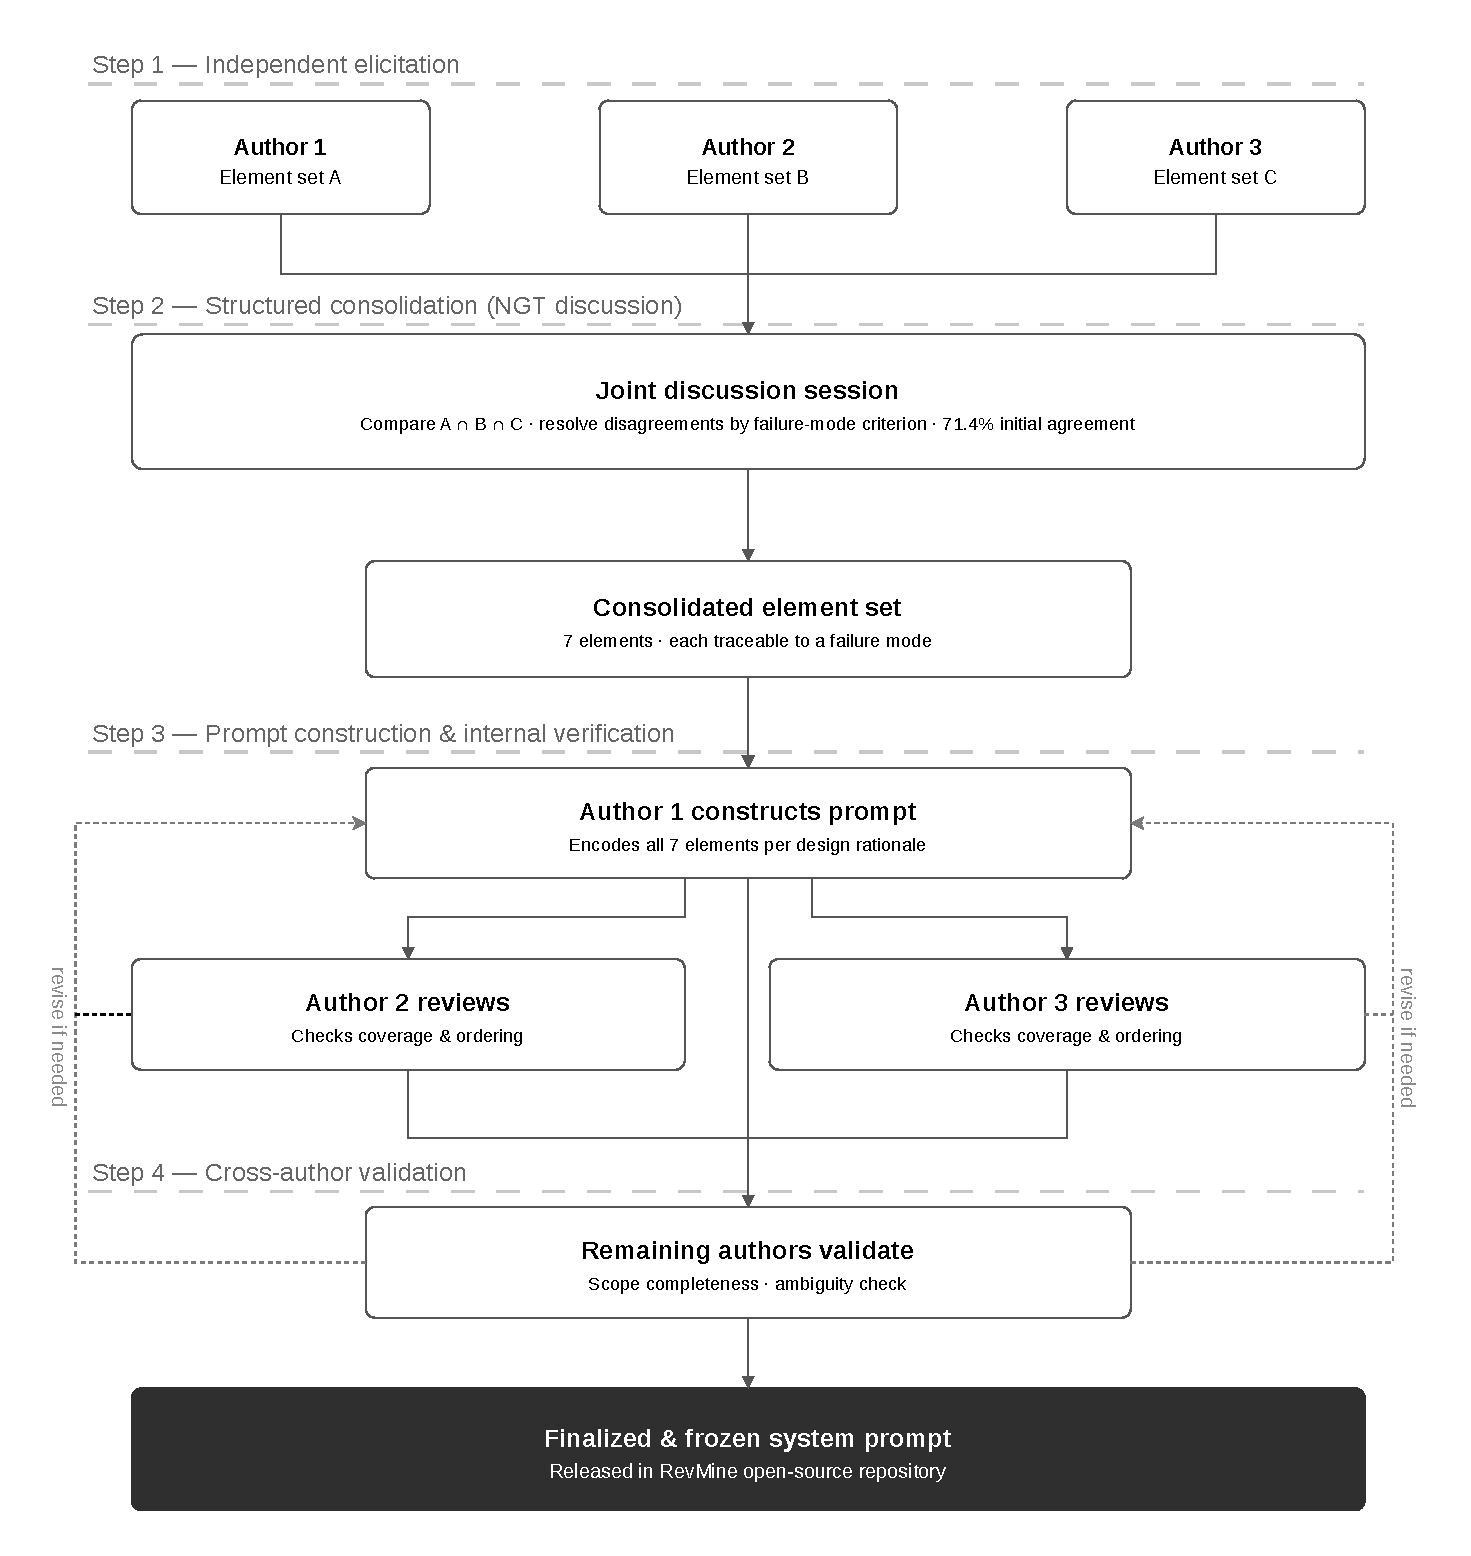
\includegraphics[width=\textwidth]{assets/ngt_revmine_diagram.pdf}
    \caption{Vue d'ensemble du processus d'ingénierie de prompts basé sur la NGT modifiée}
    \label{fig:ngt-process}
\end{figure}

\begin{enumerate}
    \item \textbf{Élicitation indépendante.} Chaque auteur identifie indépendamment les éléments
          du prompt jugés nécessaires pour l'orchestration, en utilisant le mode de configuration
          manuelle de RevMine comme spécification de référence.

    \item \textbf{Consolidation structurée.} Les ensembles produits indépendamment sont comparés
          lors d'une session de discussion structurée. Les éléments proposés ne sont retenus que
          s'ils permettent de prévenir un mode de défaillance identifié.

    \item \textbf{Construction du prompt et vérification interne.} Un auteur construit le prompt
          système à partir des décisions de conception consolidées, puis le prompt résultant est
          examiné indépendamment par les autres auteurs.

    \item \textbf{Validation croisée.} Le prompt est soumis à une passe de validation finale par
          l'ensemble des auteurs afin de confirmer qu'il reflète fidèlement le périmètre
          opérationnel complet de RevMine.
\end{enumerate}

\subsubsection*{Éléments du prompt et modes de défaillance prévenus}

Sept éléments fondamentaux ont été intégrés au prompt système à l'issue du processus NGT. Le
Tableau~\ref{tab:prompt_elements_fr} les récapitule avec les modes de défaillance correspondants.

\begin{table}[H]
\centering
\small
\caption{Éléments du prompt système et modes de défaillance prévenus}
\label{tab:prompt_elements_fr}
\begin{tabular}{|>{\raggedright\arraybackslash}p{6.5cm}
                |>{\raggedright\arraybackslash}p{6.5cm}|}
\hline
\textbf{Élément du prompt} & \textbf{Mode de défaillance prévenu} \\
\hline
Énumération fermée de toutes les métriques valides & Hallucination de noms de métriques \\
\hline
Table de dépendances métriques\,/\,features & Omission de dépendances \\
\hline
Règles de classification de l'intention & Mauvaise classification de l'intention \\
\hline
Indicateurs de détection de la plateforme & Confusion GitHub\,/\,GitLab \\
\hline
Injection dynamique de la date courante (\texttt{\_\_TODAY\_\_}) & Mauvaise résolution des expressions temporelles \\
\hline
Règles de peuplement des filtres & Filtres incorrects ou manquants \\
\hline
Instruction de discipline de sortie stricte & JSON mal formé ou encadré de texte \\
\hline
\end{tabular}
\end{table}

\subsubsection*{Modes d'exécution~: inférence locale et inférence hébergée}

Le service LLM est conçu comme \textbf{agnostique au modèle}~: la couche d'orchestration
interagit avec les LLM via une interface unifiée, permettant de substituer différents backends
sans modifier la structure du prompt ni la logique de parsing en aval.

\paragraph{Mode Ollama -- inférence locale.} Ollama est un moteur d'inférence locale permettant
d'exécuter des modèles open source (Mistral, LLaMA, Gemma, etc.) directement sur la machine hôte,
sans dépendance à un service cloud \parencite{ollama2023}. Ce mode garantit la confidentialité
totale des données et l'absence de coût par requête, au prix de performances limitées par les
ressources locales disponibles.

\paragraph{Mode OpenRouter -- modèles hébergés.} OpenRouter est une passerelle d'API agrégeant
de nombreux fournisseurs de LLM (OpenAI, Anthropic, Google, Meta, etc.) sous une interface
unifiée compatible avec l'API OpenAI \parencite{openrouter2023}. Ce mode donne accès à des
modèles de grande capacité sans infrastructure GPU requise.

Le Tableau~\ref{tab:backend_modes_fr} synthétise les compromis pratiques entre les deux modes.

\begin{table}[H]
\centering
\small
\caption{Comparaison des deux modes d'exécution du service LLM de RevMine}
\label{tab:backend_modes_fr}
\begin{tabular}{|>{\raggedright\arraybackslash}p{3.5cm}
                |>{\raggedright\arraybackslash}p{5.5cm}
                |>{\raggedright\arraybackslash}p{5.5cm}|}
\hline
\textbf{Dimension} & \textbf{Ollama (local)} & \textbf{OpenRouter (hébergé)} \\
\hline
Traitement des données & Les requêtes restent sur la machine locale & Les requêtes sont transmises à un fournisseur externe \\
\hline
Infrastructure requise & Environnement local et poids du modèle téléchargés & Connexion Internet et clé API \\
\hline
Accès aux modèles & Limité aux modèles exécutables localement & Large accès aux modèles commerciaux et open-weight \\
\hline
Confidentialité & Contrôle local fort des données & Soumis aux politiques du fournisseur externe \\
\hline
Reproductibilité & Élevée si la version du modèle est figée & Dépend de la stabilité de la version distante \\
\hline
Structure de coût & Pas de facturation par requête~; coût matériel local & Options gratuites et payantes selon le modèle \\
\hline
\end{tabular}
\end{table}

% ------------------------------------------------------------
\subsubsection{Service de notification}
% ------------------------------------------------------------

Le service de notification a été développé en \textbf{Go} avec le framework \textbf{Fiber}. Ce
choix répond à la nécessité de gérer un grand nombre de connexions WebSocket concurrentes avec
une faible empreinte mémoire, exigence difficile à satisfaire avec des frameworks synchrones
traditionnels.

Ce service consomme les événements publiés sur Kafka par les autres services, les persiste dans
sa propre base PostgreSQL, puis les diffuse en temps réel aux clients connectés via WebSocket.
L'utilisateur reçoit ainsi instantanément des informations sur l'état d'une collecte, la fin
d'un traitement ou toute anomalie survenue. Des endpoints complémentaires permettent de lister
les notifications, de comptabiliser les éléments non lus, de les marquer comme lus ou de les
supprimer.

% ============================================================
\subsection{Gestion des données et communication inter-services}
% ============================================================

La cohérence globale de RevMine repose sur une stratégie claire de gestion des données. Chaque
microservice dispose de sa propre base \textbf{PostgreSQL}, garantissant l'isolation des
responsabilités et limitant les dépendances directes entre services -- principe fondateur de
l'architecture microservices.

Les données brutes issues de la collecte sont archivées dans \textbf{MinIO} au format JSON,
séparant ainsi les artefacts bruts du stockage relationnel et facilitant leur réutilisation sans
relancer les appels API vers les plateformes distantes.

La communication entre services s'articule autour de deux mécanismes complémentaires~:

\begin{itemize}
    \item les \textbf{API REST}, pour les interactions synchrones initiées par le frontend ou
          l'API Gateway, lorsqu'une réponse immédiate est attendue~;
    \item \textbf{Apache Kafka}, comme bus de messages pour la communication asynchrone et le
          découplage des traitements internes, notamment pour les opérations longues telles que
          la collecte ou l'analyse de données.
\end{itemize}

Ces topics permettent, par exemple, au service de collecte d'informer le service d'analyse et
le service de notification de la disponibilité de nouvelles données, sans aucun couplage direct
entre eux. Le Tableau~\ref{tab:kafka-topics} détaille les topics Kafka utilisés dans la
plateforme, ainsi que leurs producteurs et consommateurs respectifs.

\begin{table}[H]
\centering
\small
\caption{Topics Kafka et flux de messages dans RevMine}
\label{tab:kafka-topics}
\begin{tabular}{|>{\raggedright\arraybackslash}p{6.2cm}
                |>{\raggedright\arraybackslash}p{3cm}
                |>{\raggedright\arraybackslash}p{3.5cm}|}
\hline
\textbf{Topic} & \textbf{Producteur} & \textbf{Consommateur(s)} \\
\hline
\texttt{config.tokens.request} & Collecte / Analyse & Configuration \\
\hline
\texttt{config.tokens.response} & Configuration & Collecte / Analyse \\
\hline
\texttt{collection.events.started} & Collecte & Notification \\
\hline
\texttt{collection.events.completed} & Collecte & Analyse, Notification \\
\hline
\texttt{collection.events.failed} & Collecte & Notification \\
\hline
\texttt{analysis.events.requested} & Analyse & Analyse \\
\hline
\texttt{analysis.events.completed} & Analyse & Notification \\
\hline
\texttt{notification.events} & Tous les services & Notification \\
\hline
\end{tabular}
\end{table}

Un message Kafka publié par le service de collecte est volontairement compact~: il transporte
l'état de la collecte, les identifiants nécessaires à la corrélation et les métadonnées utiles aux
services consommateurs, sans transporter l'intégralité des données brutes. Celles-ci restent
stockées dans MinIO.

\begin{verbatim}
{
  "event": "collection_completed",
  "collection_id": "col_42",
  "repository": "owner/project",
  "workspace_id": 7,
  "status": "completed",
  "raw_object": "revmine-collections/col_42/raw.json",
  "duration": 128.4
}
\end{verbatim}

% ============================================================
\subsection{Réalisation du frontend}
% ============================================================

Le frontend de RevMine a été développé sous la forme d'une \textbf{Single Page Application}
(SPA)\footnote{SPA (\textit{Single Page Application})~: application web qui charge une seule
page HTML au démarrage et met à jour dynamiquement le contenu sans rechargement complet de la
page, offrant une expérience utilisateur proche d'une application native.} avec \textbf{React},
offrant une navigation fluide entre les fonctionnalités.

La Figure~\ref{fig:workflow-utilisateur-revmine} synthétise le parcours cible~: l'utilisateur
exprime une demande en langage naturel, l'assistant RevMine produit un plan JSON normalisé, puis
l'exécution enchaîne collecte, stockage brut, nettoyage, analyse, visualisation et notification en
temps réel.

\begin{figure}[H]
    \centering
    \IfFileExists{assets/revmine_user_workflow.drawio.pdf}{%
        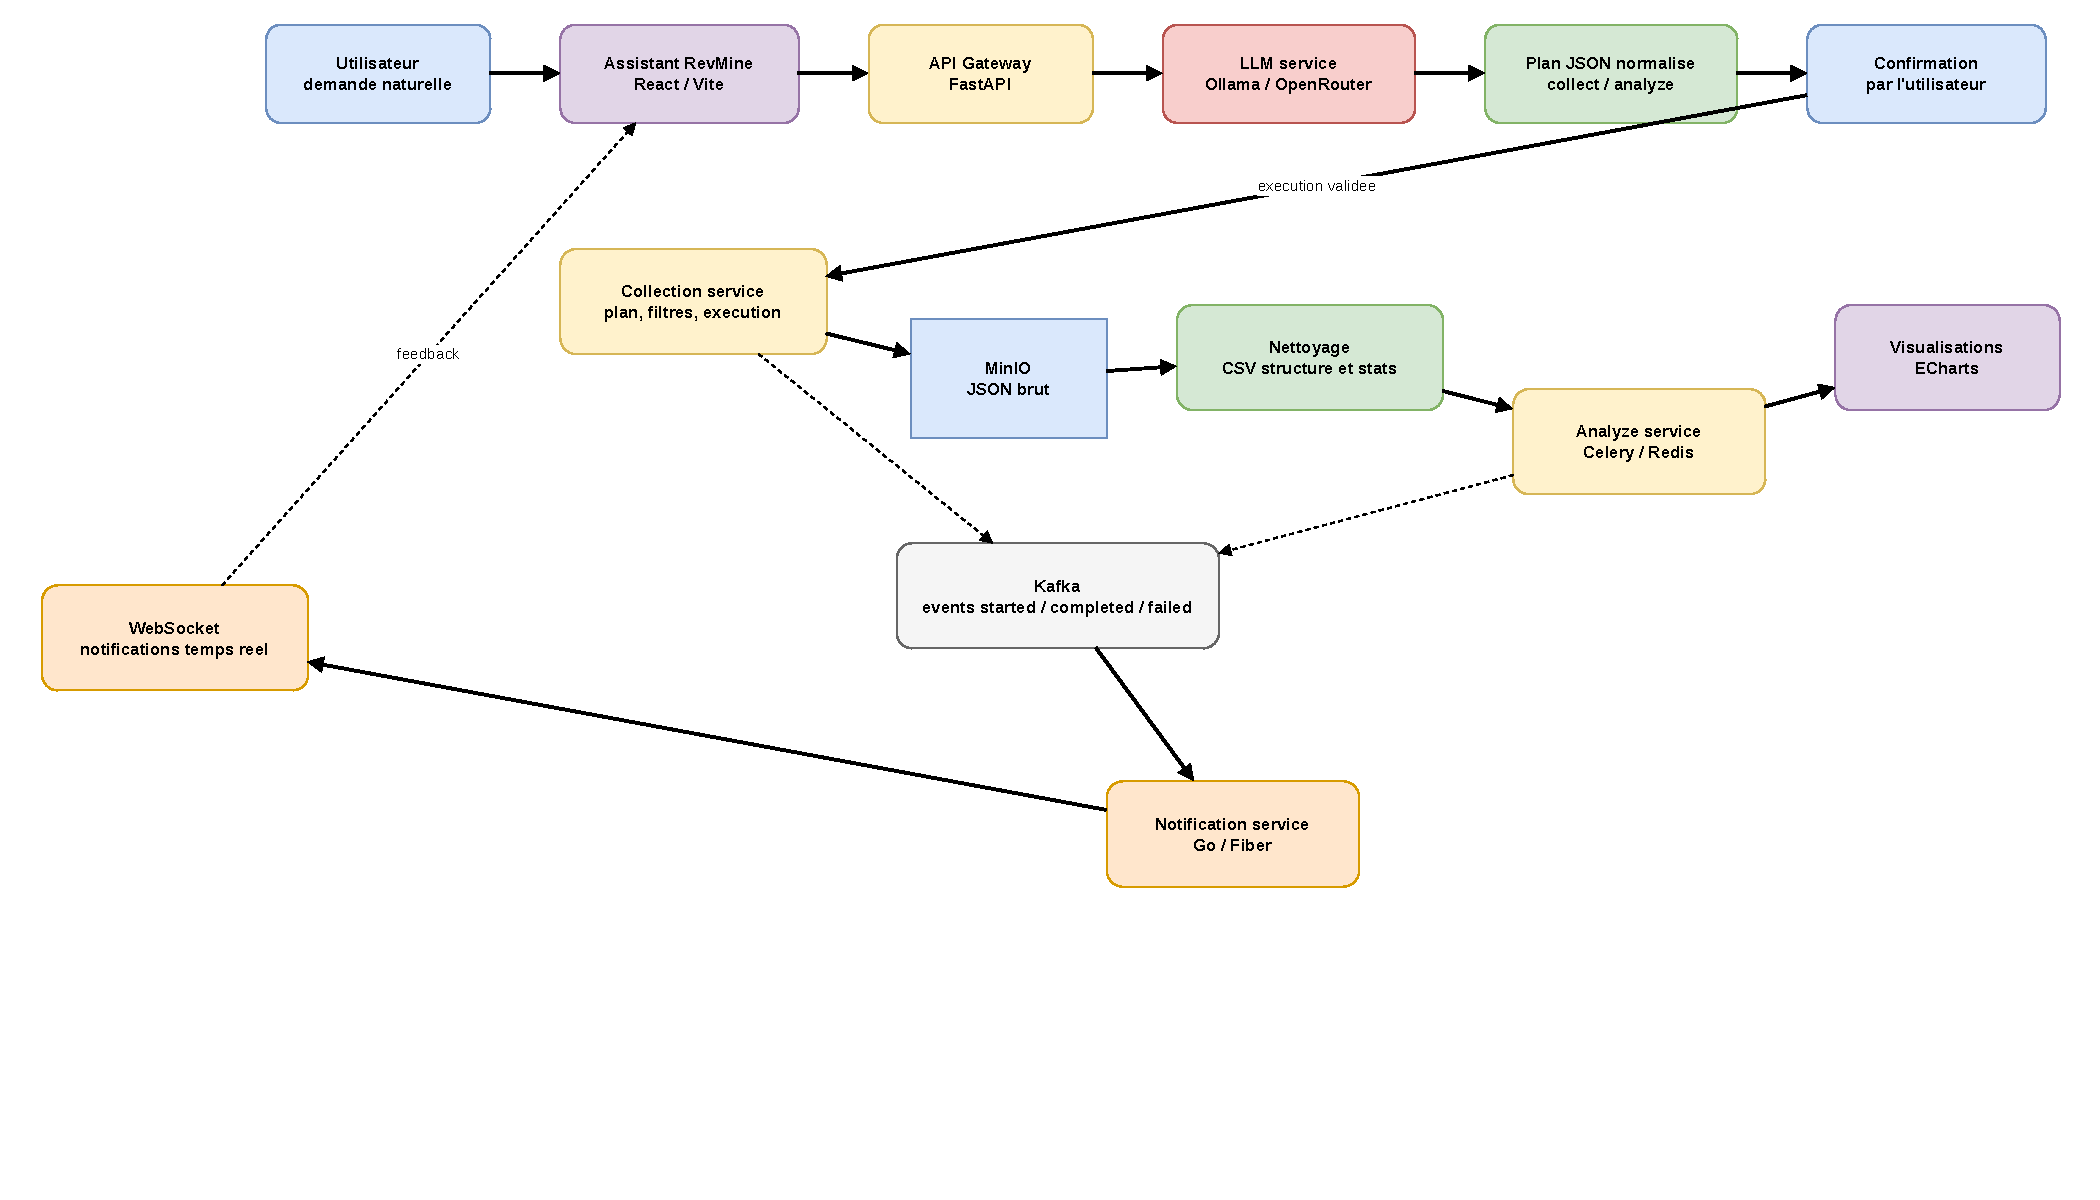
\includegraphics[width=\textwidth,height=0.55\textheight,keepaspectratio]{assets/revmine_user_workflow.drawio.pdf}%
    }{%
        \fbox{\parbox{0.9\textwidth}{\centering Diagramme de workflow à placer dans \texttt{assets/revmine\_user\_workflow.drawio.pdf}}}%
    }
    \caption{Workflow utilisateur de RevMine, de la demande naturelle à la visualisation}
    \label{fig:workflow-utilisateur-revmine}
\end{figure}

\subsubsection{Structure générale de l'interface}

La navigation est assurée par \textbf{React Router} et les vues sont organisées en pages
fonctionnelles~: authentification, gestion des workspaces, gestion des projets, collecte et
nettoyage des données, analyse, profil et paramètres. Des \textit{layouts} distincts délimitent
les espaces accessibles sans authentification et les pages réservées aux utilisateurs connectés.

\subsubsection{Gestion de l'authentification et de l'état global}

L'authentification est centralisée dans des \textit{providers} React. Lors de la connexion, les
tokens JWT sont stockés côté client et automatiquement injectés dans les en-têtes des requêtes
HTTP via des \textbf{intercepteurs Axios}. Un mécanisme de rafraîchissement silencieux évite toute
interruption de session en cas d'expiration du token d'accès. La protection des routes garantit
que les pages sensibles sont inaccessibles aux utilisateurs non authentifiés.

\subsubsection{Modules fonctionnels}

\paragraph{Gestion des workspaces et des projets.} Ce module permet à l'utilisateur de créer et
gérer ses espaces de travail, de tester la connexion à une plateforme distante et d'importer les
dépôts souhaités. L'organisation par workspace puis par dépôt reflète le processus naturel de
travail dans un environnement de développement collaboratif.

\paragraph{Collecte et nettoyage des données.} L'interface de collecte guide l'utilisateur à
travers les étapes de configuration du plan de collecte~: sélection des branches, des métriques
et des filtres. Des écrans dédiés permettent de suivre la progression de l'exécution et de
consulter les résultats. Une fois les données récupérées, des vues spécifiques donnent accès au
nettoyage, à la génération de fichiers CSV structurés et à la consultation des jeux de données
préparés.

\paragraph{Analyse et visualisation.} Le module d'analyse constitue l'une des fonctionnalités
centrales de RevMine. Il permet de lancer une analyse à partir d'un fichier CSV ou d'un dataset
préparé, de sélectionner les métriques disponibles et de générer des représentations graphiques
adaptées au contenu des données. L'interface propose également un historique des analyses et un
tableau de bord analytique. Les visualisations sont produites avec \textbf{ECharts}, une
bibliothèque graphique offrant des représentations riches et interactives.


\subsubsection{Traçabilité du parcours utilisateur}

Afin de montrer concrètement comment l'interface rend l'analyse plus accessible, le
Tableau~\ref{tab:frontend-parcours} relie les besoins utilisateur aux écrans et aux services
sollicités.

\begin{table}[H]
\centering
\small
\caption{Parcours utilisateur et services mobilisés dans RevMine}
\label{tab:frontend-parcours}
\begin{tabular}{|>{\raggedright\arraybackslash}p{3.4cm}
                |>{\raggedright\arraybackslash}p{3.2cm}
                |>{\raggedright\arraybackslash}p{3.4cm}
                |>{\raggedright\arraybackslash}p{3.4cm}|}
\hline
\textbf{Besoin utilisateur} & \textbf{Écran RevMine} & \textbf{Service appelé} & \textbf{Résultat obtenu} \\
\hline
Créer un espace de travail & Workspaces & Configuration / Authentification & Workspace associé à l'utilisateur \\
\hline
Connecter GitHub ou GitLab & Paramètres du workspace & Configuration & Token chiffré et dépôts distants disponibles \\
\hline
Formuler une demande naturelle & Assistant RevMine & API Gateway + LLM & Plan JSON normalisé proposé à l'utilisateur \\
\hline
Exécuter une collecte & Collecte & Collection + MinIO + Kafka & Données brutes JSON, état de collecte et CSV nettoyé \\
\hline
Lancer une analyse & Analyse & Analyze + Celery / Redis & Métriques calculées et graphiques ECharts \\
\hline
Suivre l'avancement & Notifications & Kafka + Notification & Notifications temps réel via WebSocket \\
\hline
\end{tabular}
\end{table}

\subsubsection{Aspects ergonomiques et visuels}

L'interface repose sur \textbf{Tailwind CSS}, qui assure la cohérence des composants, des
espacements et des couleurs, tout en garantissant un comportement adaptatif sur différentes
tailles d'écran. L'organisation modulaire des composants React et l'utilisation de contextes
partagés contribuent à la maintenabilité du code frontend.

% ============================================================
\subsection{Sécurité de la solution}
% ============================================================

La sécurité a été intégrée dès la phase de conception, selon le principe du
\textit{security by design}. Les mécanismes de protection couvrent l'ensemble des couches de
la plateforme~: API Gateway, microservices internes, stockage des secrets et interface frontend.

\subsubsection{Contrôle d'accès via l'API Gateway et le service d'authentification}

L'architecture de sécurité de RevMine sépare le \textbf{point d'entrée} et la \textbf{gestion des
identités}. L'API Gateway reçoit les requêtes du frontend et applique les contrôles transversaux,
tandis que le service d'authentification Django/DRF gère les utilisateurs et valide les JWT. Dans
l'architecture cible, les services métier ne sont pas appelés directement depuis l'extérieur~:
ils sont placés derrière la Gateway dans le réseau Docker local.

Le flux d'une requête authentifiée se déroule en quatre étapes, décrites dans le
Tableau~\ref{tab:flux-auth}~:

\begin{table}[H]
\centering
\small
\caption{Flux d'une requête authentifiée dans RevMine}
\label{tab:flux-auth}
\begin{tabular}{|>{\centering\arraybackslash}p{0.8cm}
                |>{\raggedright\arraybackslash}p{12.5cm}|}
\hline
\textbf{Étape} & \textbf{Description} \\
\hline
1 & Le frontend envoie la requête à l'API Gateway avec l'en-tête \texttt{Authorization: Bearer <token>} \\
\hline
2 & L'API Gateway transmet le JWT au service d'authentification via l'endpoint d'introspection
    \texttt{/api/auth/introspect}. En cas de token absent, invalide ou expiré, une réponse
    \texttt{401 Unauthorized} est retournée. \\
\hline
3 & Lorsque l'introspection réussit, l'API Gateway ajoute l'identifiant utilisateur
    \texttt{user\_id} à la requête interne sous la forme de l'en-tête \texttt{X-User-ID}. \\
\hline
4 & Le microservice destinataire utilise uniquement \texttt{X-User-ID} pour associer les
    ressources à l'utilisateur, sans recevoir ni manipuler le JWT complet. \\
\hline
\end{tabular}
\end{table}

\subsubsection{Isolation réseau Docker et exposition contrôlée}

Tous les composants sont rattachés au réseau Docker \texttt{revmine-network}. Les services
communiquent entre eux par leur nom de service interne~: \texttt{auth-service},
\texttt{configuration-service}, \texttt{collection-service}, \texttt{analyze-service},
\texttt{llm-service} et \texttt{notification-service}. L'exposition directe de certains ports
en environnement de développement facilite le débogage local, mais le modèle de sécurité cible
consiste à exposer les API applicatives par l'API Gateway et à considérer les autres services
comme internes. Cette contrainte est importante, car l'en-tête \texttt{X-User-ID} n'est fiable
que si les services métier ne peuvent pas être invoqués librement depuis l'extérieur.

\subsubsection{Cycle de vie des tokens JWT}

L'authentification repose sur des \textbf{tokens JWT} (RFC~7519), gérés par la bibliothèque
\textbf{django-rest-framework-simplejwt}. À l'issue d'une authentification réussie, le service
génère~: un \textbf{token d'accès} d'une durée de vie de \textbf{60~minutes}, signé avec
l'algorithme HMAC-SHA256~; et un \textbf{token de rafraîchissement} valide pendant
\textbf{7~jours}, permettant d'obtenir silencieusement un nouveau token d'accès sans
ré-authentification.

\subsubsection{Chiffrement des tokens de plateformes tierces}

Les tokens d'accès personnels fournis par l'utilisateur pour s'authentifier auprès de GitHub ou
GitLab sont chiffrés avant stockage en base de données, en utilisant l'algorithme de chiffrement
symétrique \textbf{AES-128} via l'implémentation \textbf{Fernet} de la bibliothèque Python
\texttt{cryptography}. La clé de chiffrement est conservée comme variable d'environnement,
séparée du code source et exclue du dépôt.

\subsubsection{Mécanismes de sécurité complémentaires}

Plusieurs mécanismes complémentaires renforcent la posture de sécurité globale~:
\begin{itemize}
    \item \textbf{Middlewares Django}~: \texttt{SecurityMiddleware}, \texttt{XFrameOptionsMiddleware}
          et \texttt{CsrfViewMiddleware}~;
    \item \textbf{CORS}~: les origines autorisées sont configurées via
          \texttt{CORS\_ALLOWED\_ORIGINS}~;
    \item \textbf{Validation des mots de passe}~: quatre validateurs cumulatifs (similarité au
          profil, longueur minimale, mots de passe courants, refus des mots de passe numériques)~;
    \item \textbf{Gestion des secrets par variables d'environnement}~: toutes les clés sensibles
          sont chargées via \texttt{python-decouple} depuis un fichier \texttt{.env} exclu du
          dépôt~;
    \item \textbf{Isolation des bases de données}~: chaque microservice dispose de sa propre
          instance PostgreSQL~;
    \item \textbf{Timeouts des appels proxy}~: la Gateway applique un délai maximal configuré par
          variable d'environnement afin d'éviter les requêtes bloquées indéfiniment.
\end{itemize}

% ============================================================
\section{Build}
\label{sec:build}
% ============================================================

La phase de build constitue l'étape qui transforme le code source validé en images Docker
autonomes et déployables. Dans RevMine, chaque microservice est empaquetté dans sa propre image,
garantissant l'isolation des dépendances et la reproductibilité des environnements entre le
développement, les tests et la production.

\subsection{Dockerisation des microservices}

Chaque service de RevMine dispose de son propre \texttt{Dockerfile}. Les services Python sont
principalement basés sur l'image officielle \texttt{python:3.11-slim}, le frontend sur
\texttt{node:20-alpine}, et le service de notification sur \texttt{golang:1.22-alpine}. Cette
séparation permet d'isoler les dépendances propres à chaque composant et de reconstruire un
service indépendamment des autres.

Dans les services Python, l'image installe uniquement les dépendances nécessaires, copie le code
applicatif, crée un utilisateur non privilégié et expose le port interne du service. Le service de
notification Go utilise, quant à lui, une construction \textit{multi-stage} afin de compiler le
binaire dans une image de build puis de l'exécuter dans une image Alpine plus légère. L'extrait
ci-dessous remplace avantageusement une capture d'écran de code~: il est plus lisible, vérifiable
et reste exploitable même lors d'une impression du rapport.

\begin{figure}[H]
\centering
\begin{minipage}{0.95\textwidth}
\begin{verbatim}
FROM python:3.11-slim
ENV PYTHONDONTWRITEBYTECODE=1
ENV PYTHONUNBUFFERED=1
WORKDIR /app
RUN apt-get update && apt-get install -y --no-install-recommends \
    netcat-traditional && rm -rf /var/lib/apt/lists/*
RUN groupadd --system revmine && useradd --system --gid revmine \
    --home-dir /app revmine
COPY --chmod=0444 requirements.txt .
RUN pip install --no-cache-dir -r requirements.txt
COPY --chown=revmine:revmine --chmod=0555 analytics ./analytics
USER revmine
EXPOSE 8003
CMD ["sh", "-c", "python manage.py migrate --noinput && \
     python manage.py runserver 0.0.0.0:8003"]
\end{verbatim}
\end{minipage}
\caption{Extrait représentatif du Dockerfile d'un service Python RevMine}
\label{fig:dockerfile}
\end{figure}

% ============================================================
\section{Test}
% ============================================================

\subsection{Stratégie de test}

La stratégie de test adoptée pour RevMine s'articule autour de quatre niveaux complémentaires~:

\begin{itemize}
    \item \textbf{Tests unitaires}~: vérification isolée des fonctions, classes et composants
          individuels au sein de chaque service backend et du frontend~;
    \item \textbf{Tests d'intégration}~: validation des interactions entre les couches d'un même
          service~;
    \item \textbf{Tests fonctionnels (\textit{end-to-end})}~: simulation de scénarios utilisateur
          complets dans un environnement proche de la production, à l'aide de Cypress~;
    \item \textbf{Tests de non-régression}~: exécutés automatiquement à chaque commit via le
          pipeline GitLab CI.
\end{itemize}

Les outils de test mobilisés pour chacune des couches de la plateforme sont récapitulés dans le
Tableau~\ref{tab:outils-tests}.

\begin{table}[H]
\centering
\small
\caption{Outils de test utilisés dans RevMine}
\label{tab:outils-tests}
\begin{tabular}{|>{\raggedright\arraybackslash}p{3.5cm}
                |>{\raggedright\arraybackslash}p{3.8cm}
                |>{\raggedright\arraybackslash}p{5.5cm}|}
\hline
\textbf{Couche} & \textbf{Outil} & \textbf{Périmètre couvert} \\
\hline
Backend Python & pytest + pytest-django & Tests unitaires et d'intégration \\
\hline
Service notification & go test & Tests unitaires du service temps réel écrit en Go \\
\hline
Frontend React & Jest + React Testing Library & Tests des services et composants JS \\
\hline
End-to-End & Cypress & Scénarios fonctionnels complets \\
\hline
Qualité statique & SonarQube 10.4 & Couverture, bugs, \textit{code smells} et analyse activable \\
\hline
CI/CD & GitLab CI & Automatisation des tests et build Docker \\
\hline
Couverture & Cobertura (\texttt{coverage.xml}) & Rapports de couverture par service \\
\hline
Service LLM & Benchmark (500~scénarios) & Parsing langage naturel vers JSON conforme \\
\hline
\end{tabular}
\end{table}

\subsection{Tests unitaires}

Les tests unitaires constituent le premier niveau de validation. Dans RevMine, chaque service
dispose de son propre dossier de tests, organisé en fichiers thématiques et exécuté avec l'outil
adapté à sa technologie. Les services Python utilisent \textbf{pytest}, le frontend utilise
\textbf{Jest} et le service de notification est prévu pour être validé par \textbf{go test}.
Les résultats quantitatifs et les taux de couverture associés sont présentés dans le
Chapitre~7.

\subsubsection*{API Gateway et service d'authentification}

L'API Gateway et le service d'authentification disposent de tests ciblés sur les comportements
exposés aux autres composants~: routage, limitation de débit, introspection JWT, gestion du
profil utilisateur et flux OAuth.

\begin{table}[H]
\centering
\small
\caption{Fichiers de tests de l'API Gateway et du service d'authentification}
\label{tab:tests-gateway-auth}
\begin{tabular}{|>{\raggedright\arraybackslash}p{5.2cm}
                |>{\raggedright\arraybackslash}p{8cm}|}
\hline
\textbf{Fichier de test} & \textbf{Périmètre couvert} \\
\hline
\texttt{backend/api-gateway/tests/test\_gateway.py} & Santé du service, routage public/protégé, introspection JWT, injection de l'identifiant utilisateur, limitation de débit et timeout amont \\
\hline
\texttt{backend/services/authentication/users/tests.py} & Modèle utilisateur, inscription, connexion, profil, changement de mot de passe, suppression du compte, rafraîchissement/introspection de token et OAuth GitHub/GitLab/Google \\
\hline
\end{tabular}
\end{table}

\subsubsection*{Service de configuration}

Le service de configuration dispose d'une suite de tests complète répartie sur huit fichiers,
organisés selon les couches de l'architecture propre (\textit{clean architecture}) adoptée,
comme présenté dans le Tableau~\ref{tab:tests-config}.

\begin{table}[H]
\centering
\small
\caption{Fichiers de tests du service de configuration}
\label{tab:tests-config}
\begin{tabular}{|>{\raggedright\arraybackslash}p{6cm}
                |>{\raggedright\arraybackslash}p{7cm}|}
\hline
\textbf{Fichier de test} & \textbf{Périmètre couvert} \\
\hline
\texttt{test\_api\_views.py} & Endpoints REST (CRUD workspaces et dépôts, test de connexion) \\
\hline
\texttt{test\_encryption.py} & Chiffrement et déchiffrement des tokens AES via Fernet \\
\hline
\texttt{test\_git\_infrastructure.py} & Client Git, normalisation des réponses et récupération des dépôts distants \\
\hline
\texttt{test\_kafka\_handlers.py} & Publication et consommation sur les topics \texttt{config.tokens.*} \\
\hline
\texttt{test\_repository\_service.py} & Récupération et import des dépôts depuis GitHub et GitLab \\
\hline
\texttt{test\_workspace\_rules.py} & Règles métier (unicité du nom, validation de plateforme, URL) \\
\hline
\texttt{test\_workspace\_service.py} & Cycle de vie du workspace (création, test, mise à jour) \\
\hline
\texttt{test\_workspaces.py} & Tests d'intégration des couches combinées (suite héritée) \\
\hline
\end{tabular}
\end{table}

Cette suite couvre à la fois l'ancienne surface d'intégration et les composants refactorisés,
ce qui permet de conserver la compatibilité tout en validant les nouvelles frontières
domaines/infrastructure/API.

\subsubsection*{Service de collecte}

Le service de collecte est structuré autour de fichiers de tests thématiques couvrant le domaine,
les API, les collecteurs GitHub/GitLab, MinIO, la génération CSV et les tâches asynchrones,
comme détaillé dans le Tableau~\ref{tab:tests-collection}.

\begin{table}[H]
\centering
\small
\caption{Fichiers de tests du service de collecte}
\label{tab:tests-collection}
\begin{tabular}{|>{\raggedright\arraybackslash}p{4.5cm}
                |>{\raggedright\arraybackslash}p{8.5cm}|}
\hline
\textbf{Fichier de test} & \textbf{Périmètre couvert} \\
\hline
\texttt{test\_api.py} & Endpoints REST du workflow de collecte \\
\hline
\texttt{test\_csv\_generator.py} & Génération des CSV, calculs statistiques, extraction des champs et cas limites GitHub/GitLab \\
\hline
\texttt{test\_domain.py} & Modèles de données et règles métier (\texttt{Collection}, \texttt{CleanedData}) \\
\hline
\texttt{test\_infrastructure.py} & Interactions avec MinIO (stockage et récupération de fichiers) \\
\hline
\texttt{test\_integration.py} & Flux d'exécution complets, de l'initialisation à la génération du CSV \\
\hline
\texttt{test\_services.py} & Logique des services métier (\texttt{CollectionService}, \texttt{DataCleaningService}) \\
\hline
\texttt{test\_tasks.py} & Tâches Celery, annulation, reprise, nettoyage et calcul des statistiques de collecte \\
\hline
\texttt{tests\_legacy.py} & Tests historiques conservés pour éviter les régressions sur les anciens endpoints \\
\hline
\texttt{conftest.py} & Fixtures pytest partagées (base de données de test, clients simulés) \\
\hline
\end{tabular}
\end{table}

\subsubsection*{Service d'analyse}

Le service d'analyse dispose de la suite de tests la plus étendue, organisée en quatorze fichiers
couvrant chaque couche de l'architecture, comme présenté dans le Tableau~\ref{tab:tests-analyze}.

\begin{table}[H]
\centering
\small
\caption{Fichiers de tests du service d'analyse}
\label{tab:tests-analyze}
\begin{tabular}{|>{\raggedright\arraybackslash}p{6cm}
                |>{\raggedright\arraybackslash}p{7cm}|}
\hline
\textbf{Fichier de test} & \textbf{Périmètre couvert} \\
\hline
\texttt{test\_metrics\_engine.py} & Calcul des 60+ métriques analytiques via le moteur \texttt{MetricsEngine} \\
\hline
\texttt{test\_dataset\_service.py} & Cycle de vie des datasets (création, chargement, suppression) \\
\hline
\texttt{test\_dataset\_loader.py} & Lecture CSV et détection des colonnes supplémentaires \\
\hline
\texttt{test\_analysis\_service.py} & Orchestration de l'analyse \\
\hline
\texttt{test\_analysis\_service\_new.py} & Tests complémentaires de la version refactorisée \\
\hline
\texttt{test\_analysis\_functions\_pure.py} & Fonctions analytiques pures et format des séries produites \\
\hline
\texttt{test\_celery\_tasks.py} & Tâches asynchrones Celery (déclenchement, exécution, erreurs) \\
\hline
\texttt{test\_api\_views.py} & Vues API (upload de dataset, génération de graphique, historique) \\
\hline
\texttt{test\_api.py} & Tests complémentaires des endpoints REST \\
\hline
\texttt{test\_devops\_collectors.py} & Collecteurs DevOps et normalisation des données CI/CD \\
\hline
\texttt{test\_devops\_tasks\_unit.py} & Tâches unitaires DevOps et traitements associés \\
\hline
\texttt{test\_workspace\_tokens.py} & Résolution sécurisée des tokens de workspace côté analyse \\
\hline
\texttt{test\_shim\_compatibility.py} & Compatibilité des modules shims après refactorisation \\
\hline
\texttt{test\_legacy.py} & Tests historiques des modèles et endpoints principaux \\
\hline
\end{tabular}
\end{table}

\subsubsection*{Service LLM}

Le service LLM est validé par des tests unitaires et API ciblant les deux fournisseurs supportés,
la robustesse du parsing JSON et les erreurs de modèle.

\begin{table}[H]
\centering
\small
\caption{Fichiers de tests du service LLM}
\label{tab:tests-llm}
\begin{tabular}{|>{\raggedright\arraybackslash}p{5cm}
                |>{\raggedright\arraybackslash}p{8cm}|}
\hline
\textbf{Fichier de test} & \textbf{Périmètre couvert} \\
\hline
\texttt{test\_api\_e2e.py} & Endpoints de santé, parsing, liste des modèles et erreurs HTTP contrôlées \\
\hline
\texttt{test\_json\_utils.py} & Extraction et validation d'objets JSON depuis les réponses de modèles \\
\hline
\texttt{test\_ollama\_service.py} & Appels simulés vers Ollama, erreurs de configuration et réponses invalides \\
\hline
\texttt{test\_openrouter\_service.py} & Appels simulés vers OpenRouter, clé API, erreurs réseau et réponses mal formées \\
\hline
\end{tabular}
\end{table}

\subsubsection*{Frontend}

La couche frontend est testée à l'aide de \textbf{Jest} et de \textbf{React Testing Library}.
Trois fichiers sont actuellement couverts~: \texttt{src/services/api.test.js} pour le client
HTTP Axios, \texttt{src/utils/jwt.test.js} pour la lecture des tokens JWT et
\texttt{src/context/AuthProvider.test.jsx} pour le fournisseur d'authentification React.

\subsection{Tests d'intégration}

Des bases de tests d'intégration ont été posées au sein de plusieurs services. Dans le service
de collecte, le fichier \texttt{test\_integration.py} valide le flux complet allant de
l'initialisation d'un plan de collecte à la génération du fichier CSV structuré. Dans le service
de configuration, le fichier \texttt{test\_kafka\_handlers.py} valide l'émission et la réception
de messages Kafka sur les topics \texttt{config.tokens.request} et
\texttt{config.tokens.response}.

\subsection{Tests fonctionnels (End-to-End)}

Les tests de bout en bout sont réalisés à l'aide de \textbf{Cypress}. Trois fichiers de tests
couvrent les scénarios les plus critiques de l'application, comme présenté dans le
Tableau~\ref{tab:tests-cypress}.

\begin{table}[H]
\centering
\small
\caption{Scénarios de tests fonctionnels end-to-end avec Cypress}
\label{tab:tests-cypress}
\begin{tabular}{|>{\raggedright\arraybackslash}p{4cm}
                |>{\raggedright\arraybackslash}p{9cm}|}
\hline
\textbf{Fichier Cypress} & \textbf{Scénarios couverts} \\
\hline
\texttt{auth.cy.js} & Inscription, connexion, déconnexion, refus d'accès aux routes protégées \\
\hline
\texttt{workspaces.cy.js} & Création de workspace, test de connexion, import de dépôts, suppression \\
\hline
\texttt{user-journey.cy.js} & Parcours complet~: authentification, workspace, collecte, résultats \\
\hline
\end{tabular}
\end{table}

\subsection{Qualité du code et analyse statique}

L'analyse statique est préparée avec \textbf{SonarQube Community 10.4}. La configuration est
centralisée dans \texttt{sonar-project.properties} et couvre principalement le répertoire
\texttt{backend/}, tout en excluant les migrations, les caches, les environnements virtuels, les
fichiers de tests et certains adaptateurs techniques qui ne portent pas directement la logique
métier. Les rapports de couverture produits par les jobs de test peuvent être consommés par le
scanner SonarQube.

Le Listing~\ref{lst:sonar-exclusions} présente les paramètres les plus importants de cette
configuration. Les exclusions séparent trois catégories~: les fichiers générés ou techniques
(\texttt{migrations}, caches, environnements virtuels), les fichiers de tests, et certains
adaptateurs de câblage dont la faible couverture ne reflète pas la qualité du coeur métier.

\begin{lstlisting}[caption={Extrait de configuration SonarQube pour l'analyse backend}, label={lst:sonar-exclusions}]
sonar.sources=backend

sonar.exclusions=\
  **/migrations/**,\
  **/__pycache__/**,\
  **/.venv/**,\
  **/venv/**,\
  **/node_modules/**,\
  **/schema.py,\
  **/schemas.py,\
  backend/shared/**,\
  backend/services/llm/main.py

sonar.test.inclusions=\
  **/tests/**/*.py,\
  **/tests.py,\
  **/conftest.py,\
  **/test_*.py,\
  **/*_test.py,\
  **/*_test.go

sonar.python.coverage.reportPaths=**/coverage.xml

sonar.coverage.exclusions=\
  **/tests/**,\
  **/tests.py,\
  **/conftest.py,\
  **/migrations/**,\
  **/manage.py,\
  **/asgi.py,\
  **/wsgi.py,\
  **/admin.py,\
  **/apps.py,\
  **/logging_utils.py,\
  **/kafka_utils/**
\end{lstlisting}

Le projet contient également un fichier \texttt{docker-compose.sonar.yml} permettant de démarrer
un serveur SonarQube local, sa base PostgreSQL, un conteneur de tests et un scanner. Cette
configuration rend possible l'activation d'un \textit{Quality Gate} bloquant dans un environnement
CI disposant des variables \texttt{SONAR\_HOST\_URL} et \texttt{SONAR\_TOKEN}. Dans le rapport, la
qualité statique est donc présentée comme une étape d'intégration préparée et activable, plutôt
que comme une garantie systématique lorsque le scanner n'est pas exécuté dans un pipeline donné.
La capture des résultats SonarQube est présentée dans le Chapitre~7, avec les résultats de tests
et de couverture.

% ============================================================
\section{Déploiement}
\label{sec:deploiement}
% ============================================================

Le déploiement de RevMine s'appuie sur deux piliers complémentaires~: l'orchestration des
conteneurs via \textbf{Docker Compose}, qui assure le démarrage coordonné de l'ensemble de la
stack en environnement local, et le pipeline CI/CD GitLab, qui automatise la validation et la
construction des livrables à chaque évolution du code.

\subsection{Orchestration avec Docker Compose}

Le fichier \texttt{docker-compose.yaml} est le point central de l'orchestration locale. Il
déclare les services applicatifs, les bases PostgreSQL dédiées, les composants de communication
asynchrone, le stockage objet, le service LLM local et la pile d'observabilité. Tous les services
sont rattachés au réseau Docker \texttt{revmine-network}, ce qui permet une communication interne
par nom de service.

\begin{table}[H]
\centering
\scriptsize
\caption{Services applicatifs orchestrés par Docker Compose}
\label{tab:docker-services-app}
\begin{tabular}{|>{\raggedright\arraybackslash}p{3.2cm}
                |>{\raggedright\arraybackslash}p{3.3cm}
                |>{\raggedright\arraybackslash}p{2cm}
                |>{\raggedright\arraybackslash}p{4.4cm}|}
\hline
\textbf{Service} & \textbf{Technologie} & \textbf{Port hôte} & \textbf{Rôle} \\
\hline
\texttt{frontend} & Node.js / React / Vite & \texttt{5173} & Interface utilisateur web \\
\hline
\texttt{api-gateway} & Python / FastAPI & \texttt{8000} & Point d'entrée API, routage, introspection JWT et limitation de débit \\
\hline
\texttt{auth-service} & Python / Django / DRF & \texttt{8006} & Inscription, connexion, JWT, OAuth et profil utilisateur \\
\hline
\texttt{configuration-service} & Python / Django / DRF & \texttt{8001} & Workspaces, plateformes, tokens chiffrés et dépôts importés \\
\hline
\texttt{collection-service} & Python / Django / DRF & \texttt{8002} & Collecte GitHub/GitLab, stockage brut, filtrage et génération CSV \\
\hline
\texttt{analyze-service} & Python / Django / DRF & \texttt{8003} & Datasets, métriques, analyses et visualisations \\
\hline
\texttt{celery-worker} & Python / Celery & Interne & Exécution asynchrone des traitements d'analyse \\
\hline
\texttt{llm-service} & Python / FastAPI & \texttt{8004} & Interface vers Ollama et OpenRouter \\
\hline
\texttt{notification-service} & Go / Fiber / WebSocket & \texttt{8005} & Notifications temps réel et consommation d'événements Kafka \\
\hline
\end{tabular}
\end{table}

\begin{table}[H]
\centering
\scriptsize
\caption{Services d'infrastructure orchestrés par Docker Compose}
\label{tab:docker-services-infra}
\begin{tabular}{|>{\raggedright\arraybackslash}p{3.2cm}
                |>{\raggedright\arraybackslash}p{3.3cm}
                |>{\raggedright\arraybackslash}p{2cm}
                |>{\raggedright\arraybackslash}p{4.4cm}|}
\hline
\textbf{Service} & \textbf{Image / Technologie} & \textbf{Port hôte} & \textbf{Rôle} \\
\hline
\texttt{auth-db} & PostgreSQL 15 & \texttt{5432} & Base du service d'authentification \\
\hline
\texttt{configuration-db} & PostgreSQL 15 & \texttt{5433} & Base du service de configuration \\
\hline
\texttt{collection-db} & PostgreSQL 15 & \texttt{5434} & Base du service de collecte \\
\hline
\texttt{analyze-db} & PostgreSQL 15 & \texttt{5435} & Base du service d'analyse \\
\hline
\texttt{notification-db} & PostgreSQL 15 & \texttt{5436} & Base du service de notification \\
\hline
\texttt{kafka} & Confluent Platform 7.5.0 & \texttt{9092}, \texttt{29092} & Bus d'événements en mode KRaft \\
\hline
\texttt{minio} & MinIO & \texttt{9000}, \texttt{9001} & Stockage objet des JSON bruts et console d'administration \\
\hline
\texttt{redis} & Redis 7 Alpine & \texttt{6379} & Broker Celery et stockage temporaire \\
\hline
\texttt{ollama-service} & Ollama & \texttt{11434} & Inférence LLM locale \\
\hline
\texttt{loki} & Grafana Loki & \texttt{3100} & Stockage et interrogation des journaux \\
\hline
\texttt{promtail} & Grafana Promtail & \texttt{9080} & Collecte des logs Docker et envoi vers Loki \\
\hline
\texttt{grafana} & Grafana & \texttt{3001} & Visualisation des logs et tableaux de bord \\
\hline
\end{tabular}
\end{table}

Chaque service reçoit sa configuration via les variables d'environnement du fichier \texttt{.env}
et les secrets ne sont pas intégrés aux images Docker. Les volumes Docker nommés conservent les
données des bases PostgreSQL, de MinIO, de Grafana, de Loki, de Redis, de Kafka et d'Ollama entre
les redémarrages.

Le démarrage de la stack principale s'effectue par la commande suivante~:
\begin{verbatim}
docker compose up --build
\end{verbatim}

Les points d'accès de développement les plus importants sont récapitulés dans le
Tableau~\ref{tab:docker-access}. Il faut distinguer ces ports de développement de l'architecture
cible~: pour les APIs, le point d'entrée privilégié reste l'API Gateway.

\begin{table}[H]
\centering
\small
\caption{Points d'accès locaux de la stack RevMine}
\label{tab:docker-access}
\begin{tabular}{|>{\raggedright\arraybackslash}p{4.2cm}
                |>{\raggedright\arraybackslash}p{5.1cm}
                |>{\raggedright\arraybackslash}p{4cm}|}
\hline
\textbf{Composant} & \textbf{URL locale} & \textbf{Remarque} \\
\hline
Frontend React/Vite & \texttt{http://localhost:5173} & Interface utilisateur \\
\hline
API Gateway & \texttt{http://localhost:8000} & Point d'entrée API recommandé \\
\hline
MinIO API / Console & \texttt{http://localhost:9000} / \texttt{http://localhost:9001} & Stockage objet \\
\hline
Grafana & \texttt{http://localhost:3001} & Tableaux de bord \\
\hline
Loki & \texttt{http://localhost:3100} & API de logs, utilisée par Grafana \\
\hline
Ollama & \texttt{http://localhost:11434} & Inférence locale \\
\hline
SonarQube local & \texttt{http://localhost:9090} & Via \texttt{docker-compose.sonar.yml}, hors stack principale \\
\hline
\end{tabular}
\end{table}

L'état de la stack peut être vérifié avec \texttt{docker ps}. Dans le rapport, la liste complète
des conteneurs est mieux représentée par les tableaux précédents que par une longue capture de
terminal, qui devient rapidement peu lisible à l'impression.

\subsection{Pipeline CI/CD}
\label{subsec:cicd}

Le pipeline d'intégration et de livraison continues (CI/CD\footnote{CI/CD~: \textit{Continuous
Integration / Continuous Delivery}. L'intégration continue consiste à automatiser la vérification
du code à chaque modification~; la livraison continue étend cette automatisation jusqu'à la
construction des livrables déployables.}) de RevMine est défini dans \texttt{.gitlab-ci.yml}. Il
conserve les trois étapes du cycle retenu -- \textbf{test}, \textbf{quality} et \textbf{build} --,
mais il ne repose pas sur un unique job global. Les tests et les builds sont décomposés par
service, puis déclenchés en fonction des fichiers modifiés grâce aux règles de changement. Cette
approche évite d'exécuter inutilement tous les jobs lorsqu'une modification ne concerne qu'un seul
microservice.

\begin{table}[H]
\centering
\small
\caption{Organisation du pipeline GitLab CI de RevMine}
\label{tab:pipeline-ci}
\begin{tabular}{|>{\raggedright\arraybackslash}p{2cm}
                |>{\raggedright\arraybackslash}p{5.2cm}
                |>{\raggedright\arraybackslash}p{6cm}|}
\hline
\textbf{Étape} & \textbf{Job(s)} & \textbf{Principe} \\
\hline
\texttt{test} & \makecell[l]{\texttt{test:api-gateway} \\ \texttt{test:authentication} \\ \texttt{test:configuration} \\ \texttt{test:collection} \\ \texttt{test:analyze} \\ \texttt{test:llm} \\ \texttt{test:notification}} & Exécution des tests du service concerné uniquement lorsque son code, le code partagé ou la configuration CI est modifié. \\
\hline
\texttt{quality} & \texttt{sonarqube} / scanner SonarQube & Étape préparée pour l'analyse statique. Elle peut être activée dans un environnement disposant d'un serveur SonarQube et des variables \texttt{SONAR\_HOST\_URL} et \texttt{SONAR\_TOKEN}. \\
\hline
\texttt{build} & \makecell[l]{\texttt{build:api-gateway} \\ \texttt{build:authentication} \\ \texttt{build:configuration} \\ \texttt{build:collection} \\ \texttt{build:analyze} \\ \texttt{build:llm} \\ \texttt{build:notification}} & Construction de l'image Docker du service modifié, avec une logique analogue aux jobs de test. \\
\hline
\end{tabular}
\end{table}

\paragraph{Étape de test.} Les services Python utilisent une image \texttt{python:3.11-slim} et
s'appuient sur \texttt{pytest}. Le pipeline prépare les bases de test nécessaires, installe les
dépendances du service ciblé, puis produit des rapports JUnit et Cobertura conservés comme
artefacts. Le service de notification, écrit en Go, est testé dans une image \texttt{golang} au
moyen de la commande \texttt{go test ./...}.

\paragraph{Étape d'analyse qualité.} La configuration SonarQube est présente afin de permettre
l'analyse statique et l'application d'un \textit{Quality Gate}. Cette étape dépend cependant de
la disponibilité d'un serveur SonarQube accessible par le runner. Elle doit donc être présentée
comme une intégration qualité activable selon l'environnement CI, et non comme une preuve que
chaque exécution actuelle du pipeline bloque systématiquement sur SonarQube.

\paragraph{Étape de build Docker.} Les jobs de build construisent l'image correspondant au
service modifié. Cette granularité s'aligne avec l'architecture microservices de RevMine~: une
évolution du service de collecte, par exemple, déclenche prioritairement les tests et le build de
ce service, sans reconstruire inutilement l'ensemble de la plateforme.

La Figure~\ref{fig:pipeline-passed} illustre une exécution réussie du pipeline GitLab CI. Une
capture d'échec n'est pas conservée dans le corps du rapport, car elle apporte moins d'information
qu'une description précise des règles de déclenchement et des jobs réellement exécutés.

\begin{figure}[H]
    \centering
    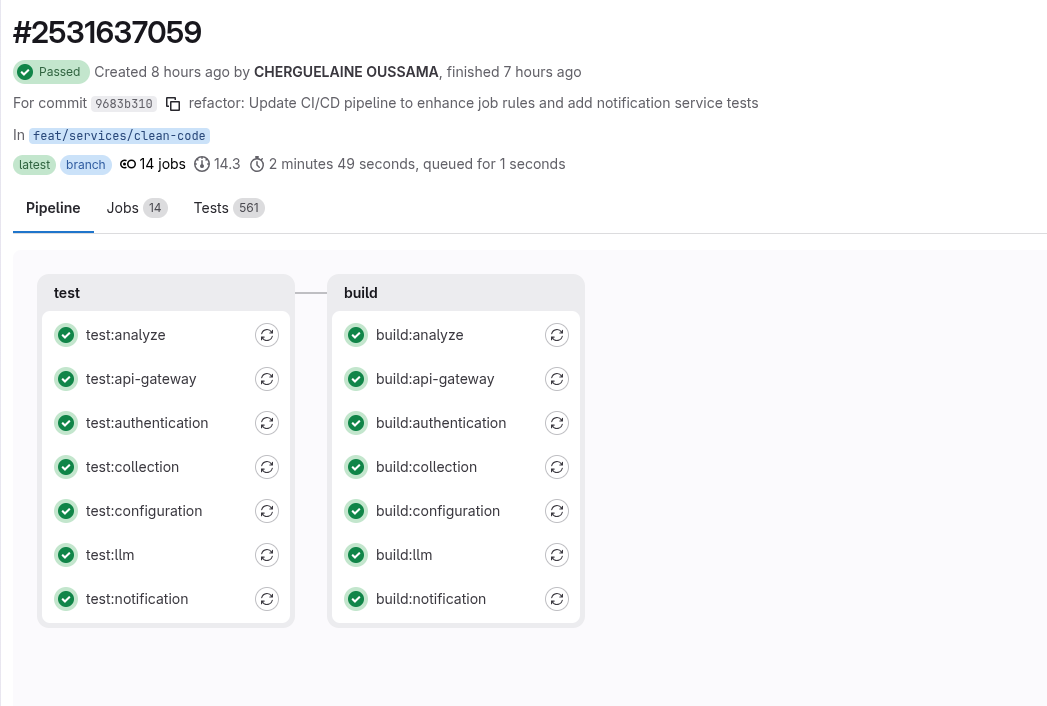
\includegraphics[width=0.95\textwidth]{captures/gitlab_pipeline_passed.png}
    \caption{Pipeline GitLab CI -- exécution réussie des jobs déclenchés par service}
    \label{fig:pipeline-passed}
\end{figure}

% ============================================================
% Section : Surveillance et Observabilité
% ============================================================
\section{Surveillance}
\label{sec:surveillance}

\subsection{Architecture d'observabilité}

La surveillance de la plateforme RevMine repose sur la pile \textbf{Loki + Promtail + Grafana},
présentée à la section~\ref{subsec:grafana-tech}. Promtail collecte les journaux des conteneurs,
Loki les stocke et les indexe par labels, puis Grafana permet leur interrogation avec le langage
LogQL. Chaque service produit des journaux en \textbf{JSON structuré}, contenant notamment le nom
du service, le niveau de sévérité, l'événement applicatif, les identifiants de corrélation et les
mesures de durée lorsque celles-ci sont disponibles.

\subsection{Indicateurs suivis dans Grafana}

Les tableaux de bord ne se limitent pas à afficher un flux de logs. Ils répondent à des besoins
opérationnels précis~: détecter un pic d'erreurs, suivre la durée des collectes, identifier les
métriques lentes, diagnostiquer les échecs et surveiller la consommation de tokens lorsque le mode
OpenRouter est utilisé. Le Tableau~\ref{tab:grafana-indicateurs} synthétise les principaux
indicateurs.

\begin{table}[H]
\centering
\scriptsize
\caption{Principaux indicateurs Grafana suivis dans RevMine}
\label{tab:grafana-indicateurs}
\begin{tabular}{|>{\raggedright\arraybackslash}p{4cm}
                |>{\raggedright\arraybackslash}p{3.2cm}
                |>{\raggedright\arraybackslash}p{6cm}|}
\hline
\textbf{Indicateur} & \textbf{Service(s)} & \textbf{Objectif} \\
\hline
Durée P95 des collectes par dépôt & \texttt{collection-service} & Détecter les dépôts dont la collecte devient anormalement longue \\
\hline
Nombre d'erreurs par service & Tous les services applicatifs & Identifier rapidement le service responsable d'un pic d'erreurs \\
\hline
Échecs de collecte par dépôt & \texttt{collection-service} & Repérer les dépôts problématiques ou les erreurs d'accès aux API GitHub/GitLab \\
\hline
Consommation de tokens OpenRouter & \texttt{llm-service} & Suivre l'utilisation des modèles cloud et maîtriser les coûts \\
\hline
Détails des échecs d'analyse & \texttt{analyze-service} & Diagnostiquer les erreurs par analyse et par métrique \\
\hline
Durée moyenne d'écriture MinIO & \texttt{collection-service} & Surveiller la performance du stockage objet \\
\hline
Échecs d'analyse par métrique & \texttt{analyze-service} & Identifier les métriques les plus souvent en erreur \\
\hline
Détails des échecs de collecte & \texttt{collection-service} & Comprendre la cause d'une collecte échouée \\
\hline
Durée moyenne de calcul par métrique & \texttt{analyze-service} & Repérer les métriques coûteuses à calculer \\
\hline
Durée médiane des collectes & \texttt{collection-service} & Suivre la performance nominale des collectes \\
\hline
Cycle de vie des collectes & \texttt{collection-service} & Suivre chronologiquement les événements \texttt{started}, \texttt{completed}, \texttt{failed} et \texttt{cancelled} \\
\hline
\end{tabular}
\end{table}

\subsection{Requêtes LogQL utilisées}

Les requêtes suivantes correspondent aux panels les plus importants des tableaux de bord Grafana.
Elles sont incluses dans le mémoire afin de rendre l'observabilité reproductible et vérifiable.

\paragraph{Durée P95 des collectes par dépôt.}
\begin{verbatim}
quantile_over_time(
  0.95,
  {service="collection-service"} | json | event="collection_completed"
    | unwrap duration [30m]
) by (repository)
\end{verbatim}

\paragraph{Nombre d'erreurs par service.}
\begin{verbatim}
sum by (service) (
  count_over_time(
    {service=~"api-gateway|configuration-service|collection-service|analyze-service|celery-worker|llm-service|notification-service"} | json | level="ERROR" [1m]
  )
)
\end{verbatim}

\paragraph{Échecs de collecte par dépôt.}
\begin{verbatim}
sum by (repository) (
  count_over_time(
    {service="collection-service"} | json | event="collection_failed" [1h]
  )
)
\end{verbatim}

\paragraph{Consommation de tokens OpenRouter.}
\begin{verbatim}
sum_over_time(
  {service="llm-service"} | json | event="llm_inference_completed" | provider="openrouter"
    | unwrap tokens_used [1m]
)
\end{verbatim}

\paragraph{Détails des échecs d'analyse.}
\begin{verbatim}
{service="analyze-service"} | json | event="analysis_failed"
  | line_format "{{.timestamp}} analysis={{.analysis_id}} metric={{.metric}} error={{.error}} duration={{.duration}}s"
\end{verbatim}

\paragraph{Durée moyenne d'écriture MinIO.}
\begin{verbatim}
avg_over_time(
  {service="collection-service"} | json | event="collection_completed"
    | unwrap minio_save_duration [10m]
)
\end{verbatim}

\paragraph{Échecs d'analyse par métrique.}
\begin{verbatim}
sum by (metric) (
  count_over_time(
    {service="analyze-service"} | json | event="analysis_failed" [1h]
  )
)
\end{verbatim}

\paragraph{Détails des échecs de collecte.}
\begin{verbatim}
{service="collection-service"} | json | event="collection_failed"
  | line_format "{{.timestamp}} repo={{.repository}} id={{.collection_id}} error={{.error}} duration={{.duration}}s"
\end{verbatim}

\paragraph{Durée moyenne de calcul par métrique.}
\begin{verbatim}
avg_over_time(
  {service="analyze-service"} | json | event="analysis_completed"
    | unwrap compute_duration [10m]
) by (metric)
\end{verbatim}

\paragraph{Durée médiane des collectes.}
\begin{verbatim}
quantile_over_time(
  0.5,
  {service="collection-service"} | json | event="collection_completed"
    | unwrap duration [30m]
)
\end{verbatim}

\paragraph{Journal du cycle de vie des collectes.}
\begin{verbatim}
{service="collection-service"} | json | event=~"collection_started|collection_completed|collection_failed|collection_cancelled"
  | line_format "{{.timestamp}} [{{.event}}] repo={{.repository}} id={{.collection_id}} status={{.status}} duration={{.duration}}s"
\end{verbatim}

\subsection{Tableaux de bord Grafana}

Les captures Grafana conservent un rôle illustratif~: elles montrent l'existence des panels et
leur intégration visuelle. L'information technique principale est toutefois fournie par les
requêtes LogQL ci-dessus, car celles-ci permettent de reproduire les graphiques et de comprendre
leur finalité.

\begin{figure}[H]
    \centering
    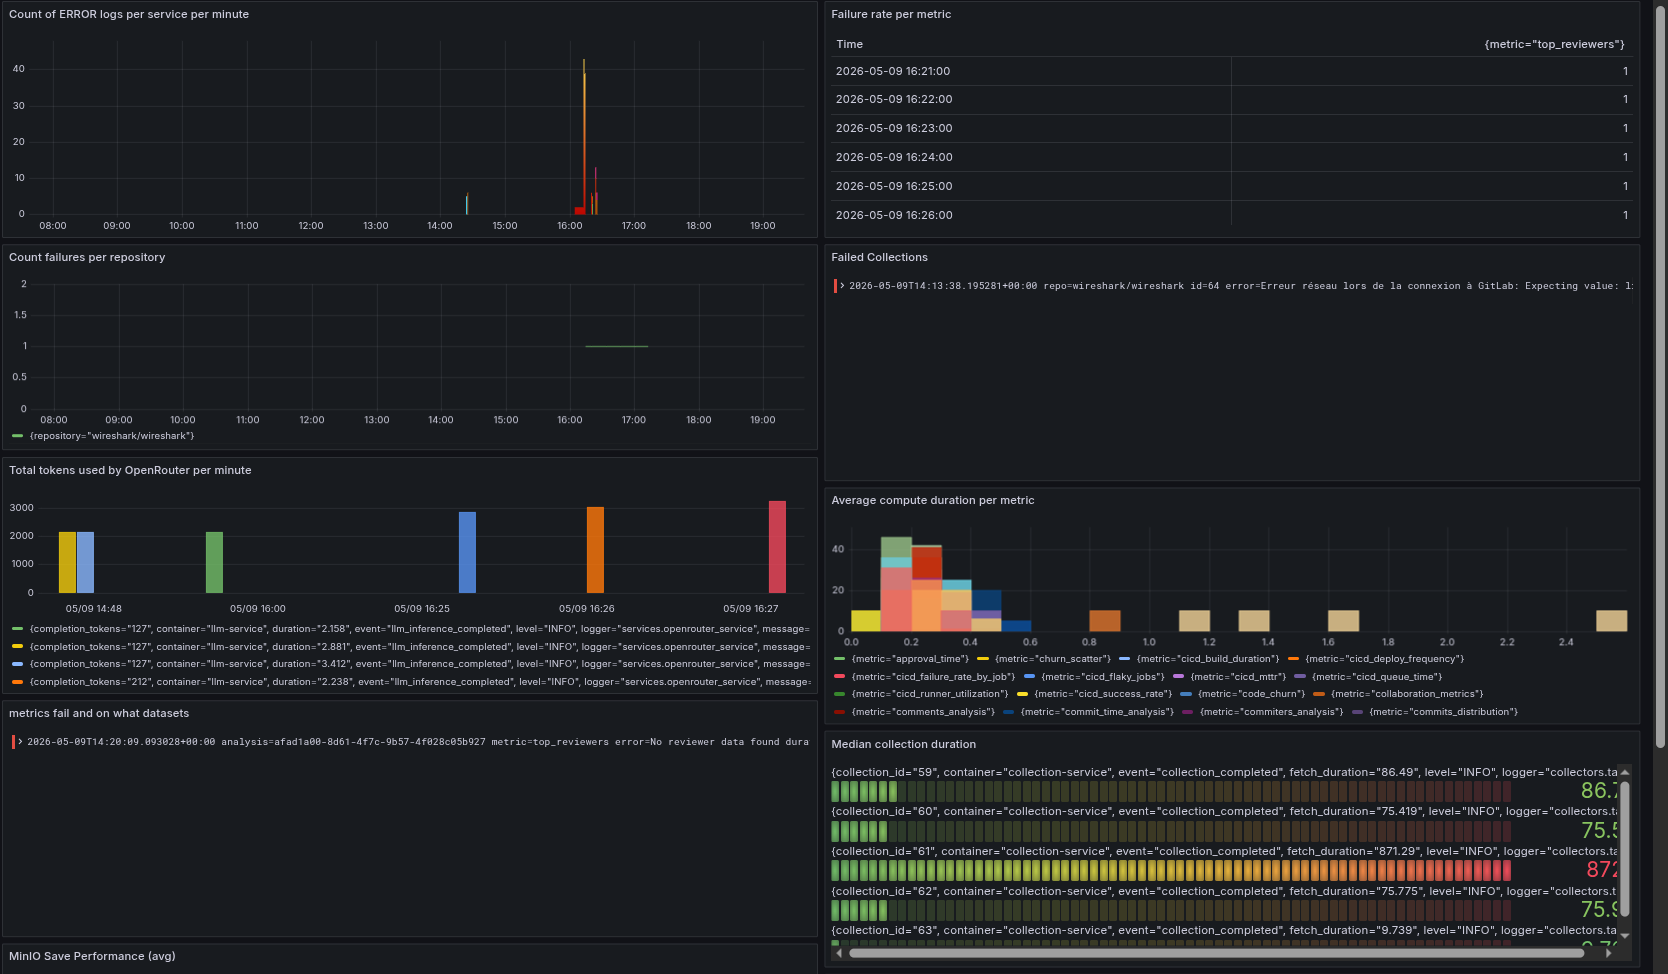
\includegraphics[width=0.95\textwidth]{captures/grafana_overview_dashboard.png}
    \caption{Tableau de bord Grafana -- vue d'ensemble de la plateforme RevMine}
    \label{fig:grafana-overview}
\end{figure}

\begin{figure}[H]
    \centering
    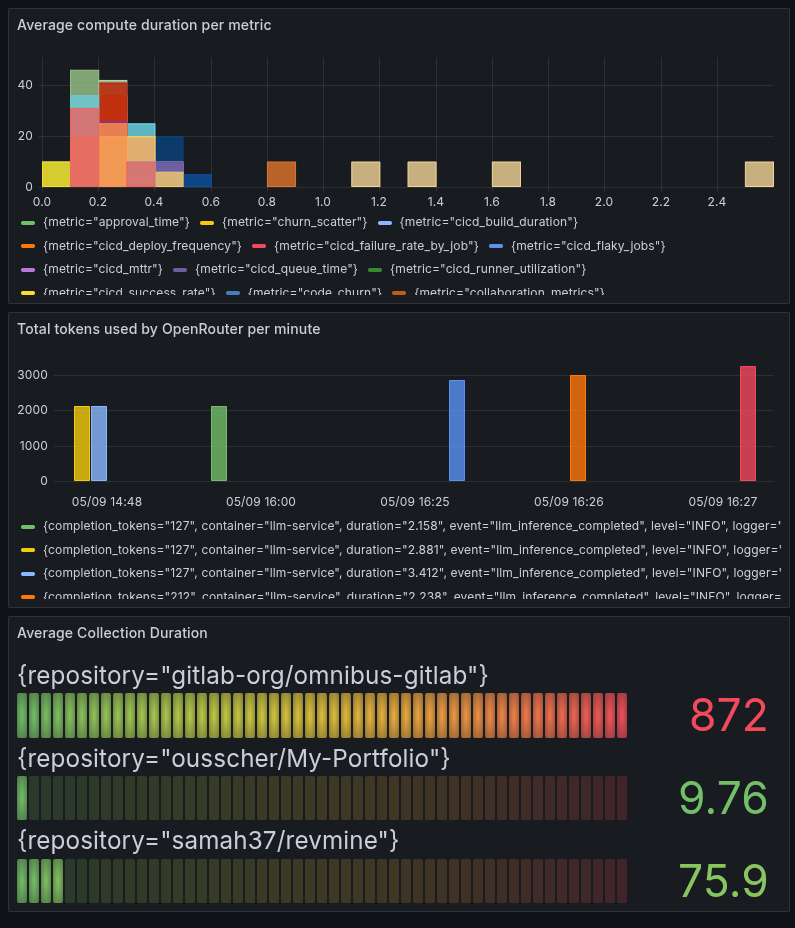
\includegraphics[width=0.95\textwidth]{captures/grafana_performance_costs.png}
    \caption{Panel Grafana -- performances des collectes, calculs d'analyse et consommation LLM}
    \label{fig:grafana-perf-costs}
\end{figure}

\begin{figure}[H]
    \centering
    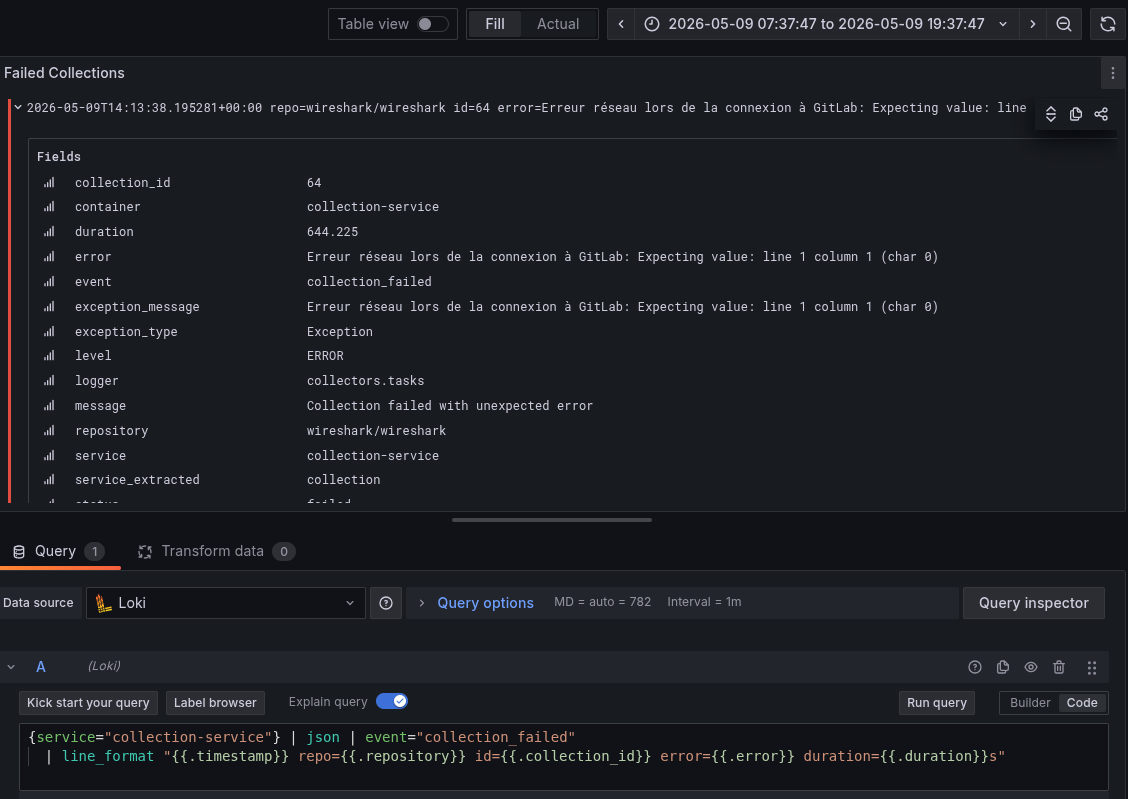
\includegraphics[width=0.95\textwidth]{captures/grafana_errors_panel.png}
    \caption{Panel Grafana -- agrégation et diagnostic des erreurs applicatives}
    \label{fig:grafana-errors}
\end{figure}

\subsection{Utilité opérationnelle}

L'observabilité mise en place répond à quatre besoins majeurs. Premièrement, elle permet une
\textbf{détection proactive} des incidents à partir des pics d'erreurs. Deuxièmement, elle
facilite l'\textbf{optimisation des performances}, en identifiant les collectes ou les métriques
les plus lentes. Troisièmement, elle contribue à la \textbf{maîtrise des coûts} lorsque les
modèles OpenRouter sont utilisés, grâce au suivi des tokens consommés. Enfin, elle renforce la
\textbf{traçabilité}, car les identifiants de collecte, d'analyse et de dépôt permettent de suivre
une opération de bout en bout.

% ============================================================
\section{Conclusion}
% ============================================================

La phase de réalisation de RevMine a permis de concrétiser l'architecture microservices définie
lors de la conception en une solution fonctionnelle, modulaire et évolutive. Développé en binôme,
le projet a bénéficié d'une organisation rigoureuse~: convention de branches justifiée, revues de
code systématiques, sprints hebdomadaires et réunions mensuelles avec l'équipe de l'ETS.

Le choix de technologies complémentaires et adaptées à chaque périmètre -- Python/Django pour les
services métier et l'authentification, FastAPI pour l'API Gateway et le service LLM, Go pour les
notifications temps réel, React pour le frontend, et la pile Grafana~+~Loki~+~Promtail pour
l'observabilité -- a permis de répondre aux exigences de performance, de maintenabilité et de
flexibilité.

Enfin, la stratégie de test multi-niveaux -- des tests unitaires aux scénarios end-to-end en
passant par l'évaluation empirique du service LLM sur 500~scénarios -- associée à la surveillance
continue via Grafana, pose les fondements d'une plateforme fiable et maintenable, capable
d'intégrer de nouvelles fonctionnalités sans compromettre la qualité de l'existant.


% =========================================================
% PARTIE III : Tests, validation et perspectives
% =========================================================
\part{Tests, validation et perspectives}

\chapter{Validation expérimentale de RevMine}
% \chapter{Validation expérimentale de RevMine}

% \label{chap:validation-experimentale}

\section{Introduction}
\label{sec:validation-introduction}

La validation de RevMine doit démontrer trois propriétés complémentaires. Premièrement, la
plateforme doit fonctionner sans régression sur ses principaux parcours techniques. Deuxièmement,
les données collectées depuis GitHub et GitLab doivent être complètes, exactes et comparables à
une vérité terrain indépendante. Troisièmement, les métriques et visualisations produites doivent
être conformes à leurs définitions mathématiques.

Ce chapitre commence donc par les résultats de tests automatisés, l'analyse statique et la
couverture de code. Il présente ensuite une démarche statistique de validation, puis l'applique à
la collecte, aux calculs analytiques, aux visualisations, à la reproductibilité et à la couche
d'orchestration LLM. L'axe méthodologique central reste la \textbf{validation différentielle par
oracle indépendant}~: les résultats produits par RevMine sont comparés à un calcul de référence
réalisé à partir des mêmes données brutes, sans réutiliser les fonctions internes de RevMine. Cette
approche suit les principes de validation des métriques logicielles, selon lesquels une mesure doit
être définie explicitement, calculée selon un protocole stable et vérifiée par rapport à l'attribut
qu'elle prétend mesurer \cite{fenton2014software,kitchenham1995framework}. La structuration des
objectifs suit également l'approche Goal--Question--Metric, qui relie chaque objectif à des
questions observables et à des métriques mesurables \cite{basili1994gqm}.

\section{Résultats des tests automatisés}
\label{sec:resultats-tests-automatises}

\subsection{Exécution des suites de tests}

Les rapports JUnit générés pour les six services Python totalisent \textbf{561~tests exécutés},
avec \textbf{0 échec}, \textbf{0 erreur} et \textbf{0 test ignoré}. En complément, les tests
unitaires frontend exécutés avec Jest totalisent \textbf{29~tests réussis} sur trois suites. Les
scénarios Cypress constituent la validation fonctionnelle de bout en bout~; ils sont conservés
comme niveau de validation globale des parcours utilisateur.

\begin{table}[H]
\centering
\small
\caption{Résultats d'exécution des tests automatisés}
\label{tab:resultats-tests-automatises}
\begin{tabular}{|>{\raggedright\arraybackslash}p{4cm}
                |>{\centering\arraybackslash}p{2.2cm}
                |>{\centering\arraybackslash}p{1.8cm}
                |>{\centering\arraybackslash}p{1.8cm}
                |>{\centering\arraybackslash}p{2cm}|}
\hline
\textbf{Service / couche} & \textbf{Outil} & \textbf{Tests} & \textbf{Échecs} & \textbf{Durée} \\
\hline
API Gateway & pytest & 7 & 0 & 2,999~s \\
\hline
Authentification & pytest & 38 & 0 & 11,153~s \\
\hline
Configuration & pytest & 111 & 0 & 3,096~s \\
\hline
Collecte & pytest & 220 & 0 & 4,633~s \\
\hline
Analyse & pytest & 161 & 0 & 37,770~s \\
\hline
Service LLM & pytest & 24 & 0 & 0,435~s \\
\hline
Frontend & Jest & 29 & 0 & 1,615~s \\
\hline
Parcours utilisateur & Cypress & 3 fichiers & à renseigner & à renseigner \\
\hline
\end{tabular}
\end{table}

Le taux de succès des tests automatisés est calculé par la formule suivante, où $N$ est le nombre
total de tests exécutés, $F$ le nombre d'échecs et $E$ le nombre d'erreurs d'exécution~:

\begin{equation}
\mathrm{TestSuccessRate} = \frac{N - F - E}{N}
\end{equation}

Pour les suites backend Python et frontend Jest exécutées, le taux observé est donc de
$100\,\%$. Les scénarios Cypress doivent être reportés avec la même logique après exécution dans
l'environnement complet, car ils valident l'enchaînement réel des écrans et des appels API.

\subsection{Couverture de code}

Le Tableau~\ref{tab:couverture} présente les derniers rapports \texttt{coverage.xml} disponibles
pour les services Python. Ces valeurs correspondent aux rapports bruts produits par pytest avant
l'application des exclusions SonarQube.

\begin{table}[H]
\centering
\small
\caption{Taux de couverture des tests backend Python par service}
\label{tab:couverture}
\begin{tabular}{|>{\raggedright\arraybackslash}p{4.5cm}
                |>{\centering\arraybackslash}p{3.2cm}
                |>{\centering\arraybackslash}p{3.2cm}
                |>{\centering\arraybackslash}p{2.8cm}|}
\hline
\textbf{Service} & \textbf{Lignes valides} & \textbf{Lignes couvertes} & \textbf{Couverture} \\
\hline
API Gateway & 137 & 128 & \textbf{93,43\,\%} \\
\hline
Authentification & 356 & 324 & \textbf{91,01\,\%} \\
\hline
Service de configuration & 687 & 589 & \textbf{85,74\,\%} \\
\hline
Service de collecte & 3\,128 & 2\,525 & \textbf{80,72\,\%} \\
\hline
Service d'analyse & 3\,018 & 2\,117 & \textbf{70,15\,\%} \\
\hline
Service LLM & 418 & 389 & \textbf{93,06\,\%} \\
\hline
\textbf{Total backend Python} & \textbf{7\,744} & \textbf{6\,072} & \textbf{78,41\,\%} \\
\hline
\end{tabular}
\end{table}

La couverture frontend n'est pas consolidée dans ce tableau, car la configuration SonarQube du
projet cible le backend. Les tests Jest valident toutefois les modules critiques actuellement
couverts côté interface~: client HTTP, décodage JWT et fournisseur d'authentification.

\section{Analyse statique et qualité du code}
\label{sec:analyse-statique-qualite}

La Figure~\ref{fig:sonar-dashboard} présente le tableau de bord SonarQube utilisé pour suivre la
qualité du backend. L'analyse ne signale aucune issue ouverte en sécurité, aucune issue ouverte
en fiabilité et aucun \textit{security hotspot}. La maintenabilité est notée A malgré
164~issues ouvertes, principalement classées comme dette technique de maintenabilité. La
couverture consolidée par SonarQube atteint \textbf{83,2\,\%} sur environ 6,4k lignes à couvrir,
et le taux de duplication est limité à \textbf{1,6\,\%}.

\begin{figure}[H]
    \centering
    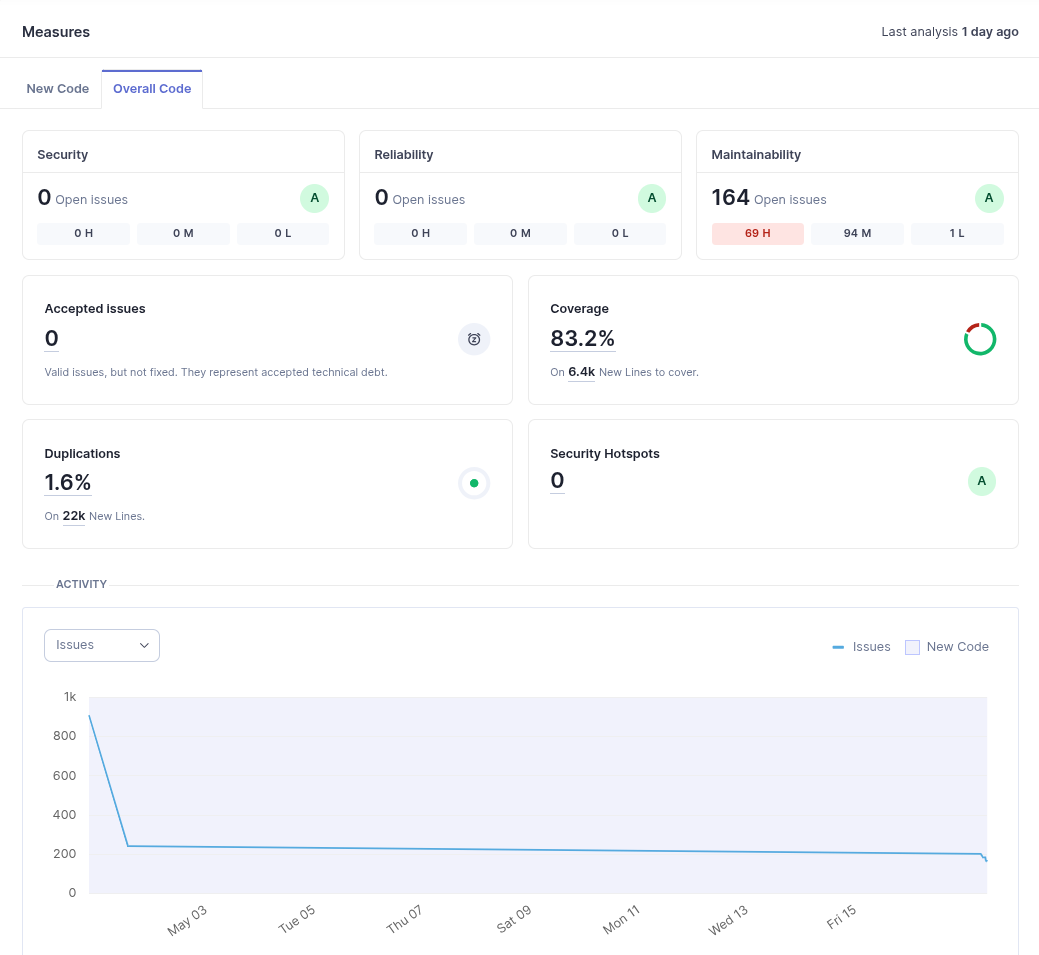
\includegraphics[width=0.95\textwidth]{captures/sonarqube_dashboard.png}
    \caption{Tableau de bord SonarQube -- métriques de qualité de RevMine}
    \label{fig:sonar-dashboard}
\end{figure}

L'écart entre la couverture brute pytest du Tableau~\ref{tab:couverture} et la couverture
SonarQube s'explique par les exclusions définies dans \texttt{sonar-project.properties}. Les
migrations, fichiers de tests, modules de démarrage, adaptateurs techniques et fichiers générés
ne sont pas considérés comme du code métier à couvrir. Cette séparation rend l'indicateur
SonarQube plus représentatif de la logique applicative réellement maintenue.

\section{Démarche de validation statistique}
\label{sec:demarche-validation-statistique}

La validation statistique de RevMine suit une démarche en trois niveaux.

\begin{enumerate}
    \item \textbf{Valider le fonctionnement global}~: vérifier que les tests unitaires,
          d'intégration et end-to-end couvrent les parcours critiques et que leur taux de succès
          est stable.
    \item \textbf{Valider la collecte avec mesure}~: comparer les entités collectées par RevMine
          avec un collecteur de référence indépendant, puis mesurer la complétude, l'exactitude et
          la cohérence multi-plateformes.
    \item \textbf{Valider l'analyse}~: comparer les métriques et séries produites par RevMine
          avec un oracle indépendant, en utilisant des mesures d'écart telles que MAE, RMSE, MAPE,
          EMR et biais moyen.
\end{enumerate}

Le Tableau~\ref{tab:questions-validation-revmine} relie ces niveaux aux questions de validation
et aux indicateurs à renseigner.

\begin{table}[H]
\centering
\small
\caption{Objectifs, questions et indicateurs de validation de RevMine}
\label{tab:questions-validation-revmine}
\begin{tabularx}{\textwidth}{|p{1.4cm}|X|X|X|}
\hline
\textbf{ID} & \textbf{Question de validation} & \textbf{Risque contrôlé} & \textbf{Indicateurs principaux} \\
\hline
QV1 & RevMine exécute-t-il correctement ses parcours techniques critiques ? & Régression fonctionnelle, route cassée, erreur d'orchestration & taux de succès des tests, réussite Cypress, erreurs applicatives \\
\hline
QV2 & RevMine collecte-t-il les entités attendues depuis GitHub et GitLab ? & Données absentes, pagination incomplète, erreur d'API ou de normalisation & FCR, FAR, CPC, taux d'erreur de champs \\
\hline
QV3 & Les métriques calculées par RevMine sont-elles conformes à leurs définitions ? & métriques temporelles, collaboratives ou de code incorrectes & EMR, MAE, RMSE, MAPE, corrélation, biais moyen \\
\hline
QV4 & Les analyses et visualisations reposent-elles sur les bonnes séries numériques ? & graphique correct visuellement mais fondé sur une agrégation erronée & exactitude des séries, distance d'agrégation, erreur relative par point \\
\hline
QV5 & Les résultats sont-ils reproductibles à paramètres constants ? & résultats différents entre deux exécutions identiques & hash des CSV normalisés, écart-type inter-exécutions, coefficient de variation \\
\hline
QV6 & La couche LLM produit-elle des plans structurés conformes au schéma RevMine ? & mauvaise intention, métriques ou dépendances manquantes & validité JSON, exact match, précision, rappel, F1, FDSR \\
\hline
\end{tabularx}
\end{table}

Les sections suivantes détaillent l'application de cette démarche à la collecte, aux métriques,
aux visualisations, à la performance, à la reproductibilité et à l'orchestration LLM.

% ============================================================
\section{Validation de la collecte de données}
\label{sec:validation-collecte}
% ============================================================

\subsection{Protocole expérimental}

La validation de la couche de collecte vise à établir l'exactitude et la complétude des données
produites par RevMine par rapport à une vérité terrain obtenue directement via les API officielles
GitHub et GitLab. Pour éviter que la vérité terrain ne soit conçue pour favoriser RevMine, le
collecteur de référence a été dérivé de la littérature existante. Un inventaire des champs et
des endpoints récupérés par des outils d'extraction établis
\parencite{gousios2017mining, bouraffa2025not, rebatchi2024dependabot, legault2022empirical,
kansab2025empirical} a permis d'implémenter un collecteur de référence récupérant l'union de
leurs surfaces de données directement depuis l'API GitHub REST (v2022-11-28) et l'API GitLab
REST (v4). Les réponses sont persistées verbatim, un fichier JSON par PR/MR, afin qu'aucun
champ retourné par l'API ne soit normalisé ou abandonné avant comparaison.

\subsection{Corpus de sujets}

Vingt dépôts open source ont été sélectionnés selon un échantillonnage raisonné
\parencite{wohlin2012experimentation} maximisant la diversité sur deux axes~: le domaine
(infrastructure, frameworks web, outils développeurs, logiciels créatifs, moteurs de jeu) et
le niveau d'activité, stratifié en trois catégories.

\begin{table}[H]
\centering
\small
\caption{Corpus de dépôts utilisés pour la validation de la collecte }
\label{tab:rq1-subjects}
\begin{tabular}{|>{\raggedright\arraybackslash}p{2cm}
                |>{\raggedright\arraybackslash}p{6.5cm}
                |>{\centering\arraybackslash}p{2cm}
                |>{\centering\arraybackslash}p{2cm}|}
\hline
\textbf{Plateforme} & \textbf{Projet} & \textbf{\#PR/MR} & \textbf{Lang.} \\
\hline
\multicolumn{4}{|l|}{\textit{Grande activité ($>$500 PR/MR par an)}} \\
\hline
GitHub & \texttt{godotengine/godot} & 55\,604 & C++ \\
GitHub & \texttt{tauri-apps/tauri} & 6\,446 & Rust \\
GitHub & \texttt{fastapi/fastapi} & 5\,625 & Python \\
GitLab & \texttt{gitlab-org/gitlab-runner} & 6\,366 & Go \\
GitLab & \texttt{gitlab-org/gitaly} & 8\,707 & Go \\
GitLab & \texttt{inkscape/inkscape} & 7\,870 & C++ \\
GitLab & \texttt{gitlab-org/omnibus-gitlab} & 9\,329 & Ruby \\
\hline
\multicolumn{4}{|l|}{\textit{Activité moyenne (100--500 PR/MR par an)}} \\
\hline
GitHub & \texttt{pallets/flask} & 2\,781 & Python \\
GitHub & \texttt{psf/black} & 2\,212 & Python \\
GitHub & \texttt{encode/httpx} & 1\,803 & Python \\
GitLab & \texttt{gitlab-org/cli} & 2\,748 & Go \\
GitLab & \texttt{gitlab-org/gitlab-docs} & 5\,354 & Markdown \\
GitLab & \texttt{gitlab-org/gitlab-development-kit} & 5\,879 & Ruby \\
\hline
\multicolumn{4}{|l|}{\textit{Faible activité ($<$100 PR/MR par an)}} \\
\hline
GitHub & \texttt{pallets/click} & 1\,458 & Python \\
GitHub & \texttt{python-attrs/attrs} & 753 & Python \\
GitHub & \texttt{sdispater/pendulum} & 369 & Python \\
GitHub & \texttt{samuelcolvin/watchfiles} & 205 & Python \\
GitLab & \texttt{gitlab-org/gitlab-triage} & 375 & Ruby \\
GitLab & \texttt{fdroid/fdroidserver} & 1\,796 & Python \\
GitLab & \texttt{inkscape/extensions} & 723 & Python \\
\hline
\end{tabular}
\end{table}

\subsection{Métriques de qualité des données}

Trois métriques de qualité des données ont été définies pour évaluer la correction de la collecte
\parencite{batini2009methodologies, kalliamvakou2014promises}.

Le \textbf{Taux de complétude des champs} (\textit{Field Completeness Rate}, FCR) mesure la
proportion d'instances de champs renseignées dans la collection de référence qui sont également
renseignées dans RevMine~:

\begin{equation}
\mathrm{FCR} =
\frac{|\{f \in P_{\mathrm{ref}} : f \text{ est renseigné dans RevMine}\}|}
     {|P_{\mathrm{ref}}|}
\end{equation}

Le \textbf{Taux de précision des champs} (\textit{Field Accuracy Rate}, FAR) mesure la
concordance exacte des valeurs sur les champs immuables, avec normalisation de chaînes (mise en
minuscules, collapse des espaces blancs)~:

\begin{equation}
\mathrm{FAR} =
\frac{\sum_{f}\mathbb{1}[\mathrm{norm}(v^{f}_{\mathrm{ref}})
         = \mathrm{norm}(v^{f}_{\mathrm{RM}})]}{|F_{\mathrm{imm}}|}
\end{equation}

La \textbf{Cohérence multi-plateformes} (\textit{Cross-Platform Consistency}, CPC) vérifie la
parité du nombre d'enregistrements, le chevauchement des identifiants et la parité des
sous-collections après alignement de la fenêtre d'évaluation.

\begin{equation}
\mathrm{CPC} =
\frac{|I_{\mathrm{RM}} \cap I_{\mathrm{ref}}|}
     {|I_{\mathrm{RM}} \cup I_{\mathrm{ref}}|}
\end{equation}

où $I_{\mathrm{RM}}$ désigne l'ensemble des identifiants collectés par RevMine et
$I_{\mathrm{ref}}$ l'ensemble des identifiants collectés par l'oracle de référence. Le même
principe est appliqué aux sous-collections critiques, par exemple les commentaires, les commits
et les fichiers modifiés.

\begin{table}[H]
\centering
\small
\caption{Synthèse des mesures de qualité de collecte}
\label{tab:resultats-qualite-collecte}
\begin{tabular}{|>{\raggedright\arraybackslash}p{2.6cm}
                |>{\centering\arraybackslash}p{1.8cm}
                |>{\centering\arraybackslash}p{2cm}
                |>{\centering\arraybackslash}p{2cm}
                |>{\centering\arraybackslash}p{2cm}
                |>{\raggedright\arraybackslash}p{3cm}|}
\hline
\textbf{Périmètre} & \textbf{Dépôts} & \textbf{FCR} & \textbf{FAR immuable} & \textbf{CPC} & \textbf{Observation} \\
\hline
GitHub & à renseigner & à renseigner & à renseigner & à renseigner & distinguer PR très volumineuses et pagination fichiers \\
\hline
GitLab & à renseigner & à renseigner & à renseigner & à renseigner & contrôler les comptes supprimés et noms miroir \\
\hline
\textbf{Global} & \textbf{20} & \textbf{100,00\,\%} & \textbf{99,85\,\%} & à renseigner & écarts résiduels documentés ci-dessous \\
\hline
\end{tabular}
\end{table}

\subsection{Résultats}

RevMine atteint une parité complète avec les scripts de collecte manuels sur GitHub et GitLab.
Sur les 20 sujets évalués, RevMine satisfait les seuils de succès à 98\,\% pour la complétude
et la précision. Les taux macro-moyennés sont $\mathrm{FCR} = 100{,}00\,\%$ et
$\mathrm{FAR} = 99{,}85\,\%$ sur les champs immuables. La complétude est parfaite sur tous les
projets~: aucun champ renseigné par le collecteur de référence n'est jamais absent de la sortie
de RevMine. La précision atteint $100{,}00\,\%$ sur 15 des 20 projets (75,0\,\%). Les 5 projets non parfaits appartiennent tous à la catégorie de grande activité et se situent entre \(98{,}02\,\%\) et \(99{,}91\,\%\), bien au-dessus du seuil de \(98\,\%\) : Godot à \(99{,}56\,\%\), GitLab Runner à \(99{,}72\,\%\), Inkscape à \(99{,}88\,\%\), Gitaly à \(99{,}91\,\%\) et Omnibus GitLab à \(98{,}02\,\%\).

L'écart résiduel de moins de 2\,\% sur ces cinq projets est exclusivement imputable à quatre
phénomènes au niveau de la plateforme, sans lien avec la logique de collecte de RevMine~:
(i)~la substitution du compte fantôme GitLab (\textit{Ghost User}, identifiant~1243277) pour
les comptes d'auteurs supprimés~; (ii)~la canonicalisation des noms d'utilisateurs en mode miroir
(suffixe~\texttt{-gtlb})~; (iii)~les modifications de titre initiées par les auteurs entre les
deux instantanés~; et (iv)~les force-push sur les branches \texttt{head} de certaines PR modifiant
le champ \texttt{head.sha} entre les deux collectes. Chacun de ces phénomènes affecterait
identiquement tout collecteur asynchrone.

Par ailleurs, la précision des champs mutables ($\mathrm{FAR}_{\mathrm{mut}}$) diminue de
manière monotone avec le délai entre les deux collectes~: de 100\,\% pour les instantanés du
même jour, jusqu'à $94{,}83\,\%$ et $95{,}66\,\%$ pour les deux paires collectées avec un
écart $\Delta t \approx 61$~jours, confirmant l'hypothèse de dérive temporelle et justifiant le
choix de persistance des réponses brutes dans MinIO pour pouvoir ré-exécuter les analyses sans
relancer les appels API.

Enfin, une limitation ponctuelle a été identifiée~: RevMine a récupéré moins d'entrées de
fichiers que le collecteur de référence sur deux très grandes PR (2\,951 contre 6\,164 pour
FastAPI~; 524 contre 4\,729 pour Godot), imputable à un plafond de pagination dans le gestionnaire
\texttt{/pulls/\{n\}/files} affectant uniquement les PR dépassant un seuil de fichiers propre
à la plateforme. Tous les autres endpoints, et toutes les collections équivalentes sur GitLab,
atteignent une parité complète. Cette limitation est documentée et sera corrigée dans la prochaine
version.

% ============================================================

\section{Validation calculatoire des métriques}
\label{sec:validation-calculatoire-metriques}

Cette section constitue l'ajout méthodologique principal. Elle vérifie la correction des métriques produites par RevMine en les comparant à un oracle de calcul indépendant. L'oracle est un script séparé, idéalement placé dans le package de réplication, qui lit les JSON bruts exportés par RevMine et recalcule les métriques sans appeler les classes internes du service d'analyse.

\subsection{Principe de l'oracle indépendant}
\label{subsec:oracle-independant}

Le protocole est le suivant :

\begin{enumerate}
    \item exécuter une collecte RevMine sur un dépôt et exporter les données brutes JSON ;
    \item calculer les métriques avec le service d'analyse RevMine ;
    \item recalculer les mêmes métriques avec un script oracle indépendant ;
    \item aligner les résultats par identifiant de PR/MR ;
    \item calculer les écarts entre RevMine et l'oracle pour chaque métrique ;
    \item documenter les divergences et leur cause : erreur de calcul, différence de définition, champ absent, pagination ou cas limite de plateforme.
\end{enumerate}

Cette validation est particulièrement adaptée à RevMine, car la contribution de la plateforme repose précisément sur la transformation de données de revue de code en métriques exploitables. Un résultat visuel convaincant n'est pas suffisant : la série numérique sous-jacente doit être vérifiée.

\subsection{Métriques à valider}
\label{subsec:metriques-a-valider}

Les métriques suivantes doivent être vérifiées en priorité, car elles structurent les analyses principales de RevMine :

\begin{table}[H]
\centering
\small
\caption{Métriques RevMine à valider par oracle indépendant}
\label{tab:metriques-oracle-validation}
\begin{tabularx}{\textwidth}{|p{3.2cm}|X|X|}
\hline
\textbf{Métrique} & \textbf{Définition de référence} & \textbf{Type de comparaison} \\
\hline
Lead time & durée entre création et fusion ou fermeture de la PR/MR & erreur absolue en secondes ou minutes \\
\hline
Review time & durée entre la création de la PR/MR et le premier commentaire, la première revue ou l'approbation selon la définition retenue & erreur absolue et vérification des événements utilisés \\
\hline
Nombre de commentaires & nombre de commentaires associés à la PR/MR, selon les catégories incluses & correspondance exacte \\
\hline
Nombre de reviewers & nombre d'acteurs distincts ayant participé à la revue & correspondance exacte sur ensemble d'identifiants \\
\hline
Code churn & additions $+$ suppressions, ou additions et suppressions séparées selon le schéma & correspondance exacte \\
\hline
Nombre de fichiers modifiés & cardinalité de la liste des fichiers associés à la PR/MR & correspondance exacte \\
\hline
Rework size & volume de modifications postérieures au premier retour de revue & erreur absolue, car dépend de l'horodatage du premier retour \\
\hline
Entropie historique & dispersion des modifications sur les fichiers ou zones du dépôt & erreur numérique avec tolérance \\
\hline
\end{tabularx}
\end{table}

\subsection{Mesures d'écart}
\label{subsec:mesures-ecart}

Pour une métrique numérique $m$, on note $y_i$ la valeur produite par l'oracle et $\hat{y}_i$ la valeur produite par RevMine pour la PR/MR $i$. L'erreur absolue moyenne est :

\begin{equation}
\mathrm{MAE}(m) = \frac{1}{n}\sum_{i=1}^{n}|\hat{y}_i-y_i|
\end{equation}

La racine de l'erreur quadratique moyenne est :

\begin{equation}
\mathrm{RMSE}(m) = \sqrt{\frac{1}{n}\sum_{i=1}^{n}(\hat{y}_i-y_i)^2}
\end{equation}

Pour les métriques strictement positives, l'erreur absolue relative moyenne est :

\begin{equation}
\mathrm{MAPE}(m) = \frac{100}{n}\sum_{i=1}^{n}\left|\frac{\hat{y}_i-y_i}{y_i}\right|
\end{equation}

Pour les métriques discrètes ou catégorielles, le taux de correspondance exacte est :

\begin{equation}
\mathrm{EMR}(m) = \frac{|\{i \mid \hat{y}_i=y_i\}|}{n}
\end{equation}

Lorsque deux méthodes de mesure sont comparées, une corrélation élevée ne suffit pas à prouver l'accord entre elles. Une analyse des différences, de type Bland--Altman, peut être utilisée pour inspecter le biais moyen et les limites d'accord \cite{bland1986statistical}. Le biais moyen est :

\begin{equation}
\mathrm{Bias}(m) = \frac{1}{n}\sum_{i=1}^{n}(\hat{y}_i-y_i)
\end{equation}

Les limites d'accord à 95\% sont approximées par :

\begin{equation}
\mathrm{LoA}_{95\%} = \mathrm{Bias} \pm 1.96 \times \sigma_{d}
\end{equation}

où $\sigma_d$ est l'écart-type des différences $d_i=\hat{y}_i-y_i$.

\subsection{Seuils d'acceptation}
\label{subsec:seuils-acceptation}

Les seuils doivent être définis avant l'exécution de l'expérience afin d'éviter une interprétation opportuniste des résultats. Les seuils suivants sont proposés :

\begin{table}[H]
\centering
\small
\caption{Seuils d'acceptation proposés pour la validation calculatoire}
\label{tab:seuils-validation-calculatoire}
\begin{tabularx}{\textwidth}{|p{3.5cm}|X|X|}
\hline
\textbf{Type de métrique} & \textbf{Indicateur} & \textbf{Seuil proposé} \\
\hline
Comptages exacts & EMR & $\geq 99\%$ hors cas de plateforme documentés \\
\hline
Durées temporelles & MAE & $\leq 60$ secondes si les timestamps sont à la seconde, ou $0$ si la précision est identique \\
\hline
Métriques de code & EMR ou MAPE & EMR $\geq 99\%$ pour additions/suppressions ; MAPE $\leq 1\%$ si agrégation approximée \\
\hline
Entropie & erreur absolue moyenne & $\leq 10^{-6}$ si la formule est identique ; sinon justifier l'écart de définition \\
\hline
Visualisations & exactitude de la série agrégée & $\geq 99\%$ de points identiques ou erreur relative $\leq 1\%$ \\
\hline
Reproductibilité & hash des CSV normalisés & identité stricte pour données figées ; sinon expliquer les champs volatils \\
\hline
\end{tabularx}
\end{table}

\subsection{Tableau de résultats à intégrer}
\label{subsec:tableau-resultats-calculatoire}

Le tableau suivant doit être rempli après exécution de l'oracle. Il est préférable de rapporter les résultats par métrique et par plateforme, puis de donner une synthèse globale.

\begin{table}[H]
\centering
\small
\caption{Résultats de validation calculatoire des métriques}
\label{tab:resultats-validation-calculatoire}
\begin{tabularx}{\textwidth}{|p{2.6cm}|p{1.5cm}|p{1.5cm}|p{1.5cm}|p{1.6cm}|X|}
\hline
\textbf{Métrique} & \textbf{Plateforme} & \textbf{EMR} & \textbf{MAE} & \textbf{MAPE} & \textbf{Interprétation} \\
\hline
Lead time & GitHub & à renseigner & à renseigner & à renseigner & vérifier les fuseaux horaires et timestamps \\
\hline
Lead time & GitLab & à renseigner & à renseigner & à renseigner & vérifier les états fermée/fusionnée \\
\hline
Commentaires & GitHub & à renseigner & à renseigner & à renseigner & distinguer commentaires généraux et commentaires de revue \\
\hline
Commentaires & GitLab & à renseigner & à renseigner & à renseigner & vérifier les notes système et commentaires utilisateur \\
\hline
Code churn & GitHub & à renseigner & à renseigner & à renseigner & contrôler les PR/MR très volumineuses \\
\hline
Code churn & GitLab & à renseigner & à renseigner & à renseigner & contrôler la pagination des changements \\
\hline
Entropie historique & multi-plateforme & à renseigner & à renseigner & à renseigner & documenter la formule utilisée \\
\hline
\end{tabularx}
\end{table}

\section{Validation des analyses et visualisations}
\label{sec:validation-visualisations}

La validation des visualisations vérifie que les graphiques affichés par RevMine correspondent exactement aux séries de données attendues. Il ne s'agit pas d'évaluer l'esthétique de l'interface, mais de vérifier les agrégations numériques.

Pour chaque visualisation, on compare la série produite par l'API d'analyse RevMine avec une série de référence calculée par l'oracle. Pour une série temporelle $S$ comportant $k$ points, l'erreur relative moyenne par point est :

\begin{equation}
\mathrm{MRE}_{series} = \frac{1}{k}\sum_{j=1}^{k}\left|\frac{\hat{s}_j-s_j}{\max(|s_j|,\epsilon)}\right|
\end{equation}

où $\epsilon$ évite une division par zéro. Une visualisation est considérée comme valide si la série des abscisses, la série des ordonnées et la règle d'agrégation correspondent à la spécification.

\begin{table}[H]
\centering
\small
\caption{Validation des visualisations par comparaison de séries}
\label{tab:validation-visualisations}
\begin{tabularx}{\textwidth}{|p{3cm}|X|X|X|}
\hline
\textbf{Analyse} & \textbf{Série de référence} & \textbf{Comparaison} & \textbf{Critère d'acceptation} \\
\hline
Commits over time & nombre de commits par période & comparaison point par point & série identique ou MRE $\leq 1\%$ \\
\hline
Timeline PR/MR & nombre de PR/MR créées par période & comparaison des buckets temporels & buckets et valeurs identiques \\
\hline
Distribution du lead time & histogramme ou distribution des durées & comparaison des classes et effectifs & classes identiques et EMR $\geq 99\%$ \\
\hline
Top contributeurs & classement par nombre de contributions & comparaison du rang et du score & top-$k$ identique ou recouvrement $\geq 95\%$ \\
\hline
Matrice de corrélation & corrélations entre métriques numériques & différence absolue moyenne & erreur $\leq 10^{-6}$ si même formule \\
\hline
\end{tabularx}
\end{table}

\section{Validation de performance et de passage à l'échelle}
\label{sec:validation-performance}

La performance doit être évaluée sur les mêmes dépôts que la validation de collecte, en enregistrant les temps de début et de fin, le volume de données, le nombre d'appels API et les ressources consommées. Les métriques suivantes sont proposées.

Le débit de collecte est défini par :

\begin{equation}
\mathrm{Throughput} = \frac{N_{items}}{T_{collecte}}
\end{equation}

où $N_{items}$ est le nombre d'entités collectées et $T_{collecte}$ le temps total en minutes.

L'efficacité API est définie par :

\begin{equation}
\mathrm{API\ Efficiency} = \frac{N_{items}}{N_{api\ calls}}
\end{equation}

Le taux de reprise après interruption est défini par :

\begin{equation}
\mathrm{Resume\ Consistency} = \frac{|E_{normal} \cap E_{resumed}|}{|E_{normal}|}
\end{equation}

où $E_{normal}$ est l'ensemble collecté en exécution normale et $E_{resumed}$ l'ensemble obtenu après interruption puis reprise.

\begin{table}[H]
\centering
\small
\caption{Indicateurs de performance et de robustesse opérationnelle}
\label{tab:validation-performance}
\begin{tabularx}{\textwidth}{|p{3.4cm}|X|X|}
\hline
\textbf{Indicateur} & \textbf{Définition} & \textbf{Interprétation} \\
\hline
Temps total de collecte & durée entre le lancement et la fin de la collecte & mesure l'effort opérationnel \\
\hline
Débit & entités collectées par minute & compare petits et grands dépôts \\
\hline
Efficacité API & entités collectées par appel API & mesure la qualité de pagination et de batch \\
\hline
Taux d'échec & collectes échouées sur collectes lancées & mesure la robustesse générale \\
\hline
Cohérence de reprise & similarité entre collecte normale et collecte reprise & vérifie la reprise après interruption \\
\hline
Consommation mémoire & pic mémoire par service & détecte les limites de scalabilité \\
\hline
\end{tabularx}
\end{table}

\section{Validation de reproductibilité}
\label{sec:validation-reproductibilite}

La reproductibilité est essentielle pour un outil destiné à l'ingénierie logicielle empirique. Pour une même configuration, une même période et un même dépôt figé, RevMine doit produire le même dataset, modulo les champs volatils tels que les dates d'exécution ou les identifiants internes.

Le protocole recommandé est le suivant :

\begin{enumerate}
    \item exécuter la même collecte trois fois avec les mêmes paramètres ;
    \item normaliser les fichiers exportés en retirant les champs volatils ;
    \item trier les lignes par identifiant stable de PR/MR ;
    \item calculer un hash SHA-256 de chaque CSV normalisé ;
    \item comparer les métriques agrégées entre exécutions.
\end{enumerate}

Le coefficient de variation d'une métrique $m$ sur $r$ exécutions est :

\begin{equation}
\mathrm{CV}(m) = \frac{\sigma(m)}{\mu(m)}
\end{equation}

Un coefficient de variation nul ou très proche de zéro indique une reproductibilité forte. Toute différence doit être expliquée par une modification réelle des données de la plateforme, par un champ non déterministe ou par une limite de l'API.

\section{Évaluation de la couche d'orchestration LLM}
\label{sec:eval-llm}
% ============================================================

\subsection{Objectifs et protocole}

La couche d'orchestration LLM de RevMine répond à une problématique de \textbf{traduction
sémantique}~: l'utilisateur formule une requête en langage naturel, et le service doit en extraire
un plan de collecte structuré, valide et conforme au schéma de la plateforme. Contrairement aux
services métier classiques dont la logique est déterministe, la sortie d'un modèle de langage est
probabiliste. L'évaluation repose donc sur une approche empirique fondée sur un benchmark annoté
manuellement.

\subsubsection{Benchmark de 500~scénarios}

Un benchmark de \textbf{500~scénarios} a été constitué manuellement. Chaque scénario associe une
requête en langage naturel à sa sortie JSON de référence, conforme au schéma de RevMine. La
construction a été répartie entre les auteurs (100, 200 et 200~scénarios respectivement) pour
diversifier les formulations et les intentions exprimées~; une passe de vérification croisée a
ensuite assuré la cohérence des annotations, en vérifiant la validité du schéma, la cohérence
d'interprétation des champs et l'alignement entre requête et réponse attendue.

\subsubsection{Cadre d'évaluation}

Comme illustré dans la Figure~\ref{fig:eval-framework}, tous les modèles sélectionnés ont été
évalués selon le même prompt d'orchestration, la même structure de requête et la même procédure
de scoring.

\begin{figure}[H]
    \centering
    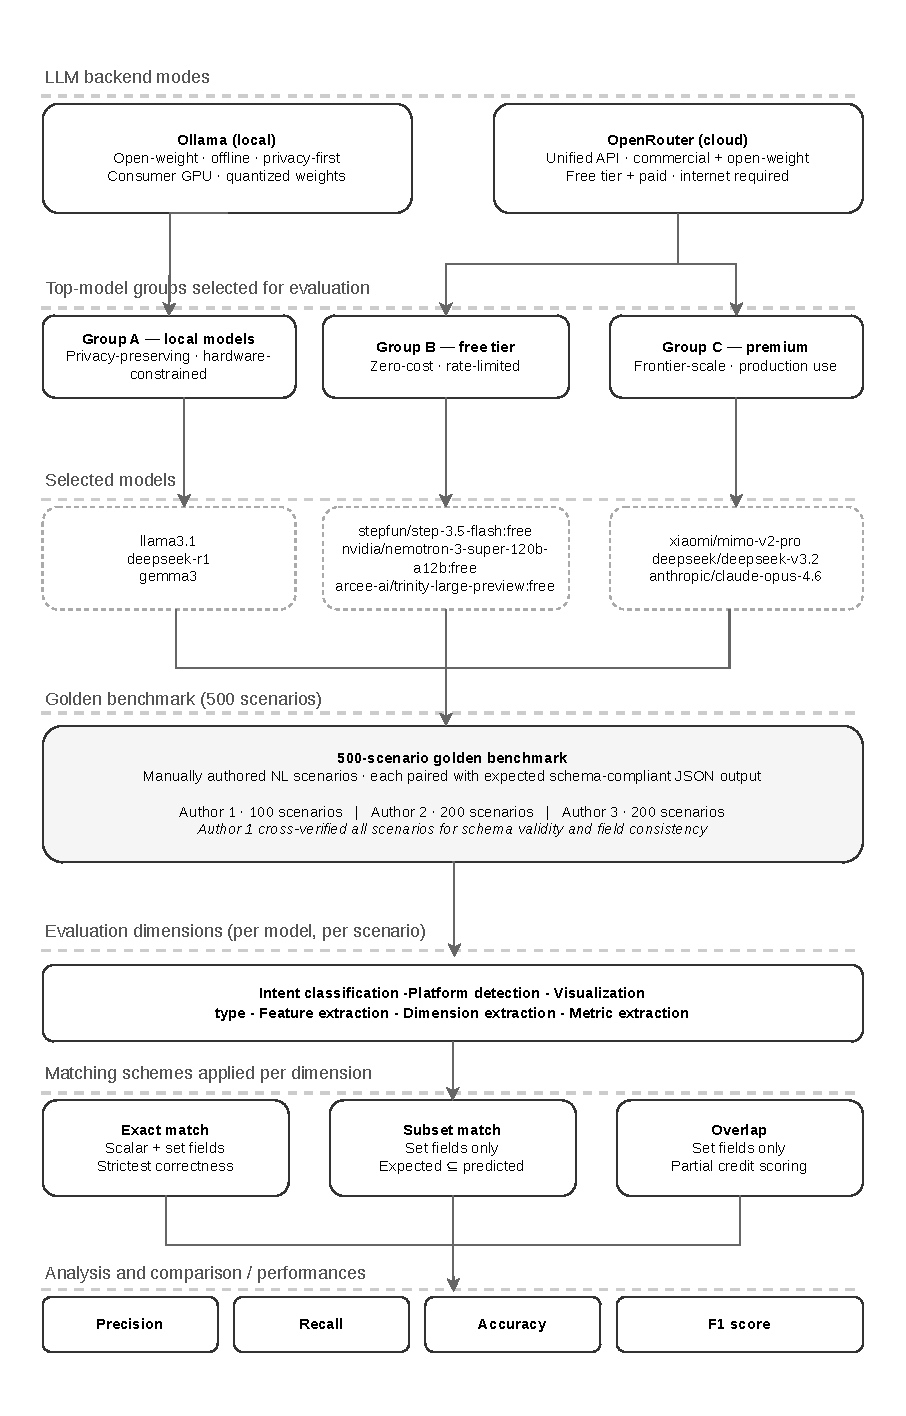
\includegraphics[width=\textwidth]{assets/evaluation_framework.pdf}
    \caption{Vue d'ensemble du cadre d'évaluation de la couche LLM de RevMine}
    \label{fig:eval-framework}
\end{figure}

L'évaluation porte sur six \textbf{dimensions}, chacune correspondant à un champ du schéma JSON
et à un mode de défaillance identifié lors de l'ingénierie des prompts.

\begin{table}[H]
\centering
\small
\caption{Dimensions d'évaluation de la couche LLM et impact opérationnel des erreurs}
\label{tab:eval_dim_fr}
\begin{tabular}{|>{\raggedright\arraybackslash}p{3.5cm}
                |>{\centering\arraybackslash}p{1.8cm}
                |>{\raggedright\arraybackslash}p{7cm}|}
\hline
\textbf{Dimension (champ JSON)} & \textbf{Type} & \textbf{Impact en cas d'erreur} \\
\hline
Intention (\texttt{intent}) & Scalaire & Critique~: mauvais pipeline déclenché \\
\hline
Plateforme (\texttt{platform}) & Scalaire & Élevé~: appels API vers la mauvaise source \\
\hline
Visualisation (\texttt{visualization}) & Scalaire & Moyen~: graphique inadapté \\
\hline
Métriques (\texttt{metrics}) & Ensemble & Critique~: lacunes silencieuses ou noms rejetés \\
\hline
Features (\texttt{features}) & Ensemble & Élevé~: colonnes absentes du dataset de sortie \\
\hline
Dimensions analytiques (\texttt{dimensions}) & Ensemble & Moyen~: agrégations incohérentes \\
\hline
\end{tabular}
\end{table}

Les champs scalaires sont évalués par \textbf{correspondance exacte}. Les champs ensemblistes sont
évalués selon trois critères~: correspondance exacte (ensemble prédit identique à l'ensemble
attendu), correspondance par sous-ensemble (tous les éléments attendus sont présents), et métriques
de recouvrement (précision, rappel, F\textsubscript{1}).

\subsubsection{Modèles évalués}

Neuf modèles ont été évalués, organisés en trois groupes reflétant les principaux contextes de
déploiement de RevMine~: modèles locaux via Ollama (Groupe~A), modèles hébergés gratuits via
OpenRouter (Groupe~B) et modèles premium via OpenRouter (Groupe~C).

\begin{table}[H]
\centering
\small
\caption{Correspondance des abréviations des modèles évalués}
\label{tab:rq2_abbrev_fr}
\begin{tabular}{|>{\raggedright\arraybackslash}p{4cm}
                |>{\raggedright\arraybackslash}p{9cm}|}
\hline
\textbf{Abréviation} & \textbf{Identifiant complet} \\
\hline
\texttt{llama-3.1-8b}    & \texttt{meta-llama/llama-3.1-8b-instruct} \\
\hline
\texttt{gemma-3-27b}     & \texttt{google/gemma-3-27b-it} \\
\hline
\texttt{deepseek-r1}     & \texttt{deepseek/deepseek-r1} \\
\hline
\texttt{step-3.5-flash}  & \texttt{stepfun/step-3.5-flash:free} \\
\hline
\texttt{nemotron-120b}   & \texttt{nvidia/nemotron-3-super-120b-a12b:free} \\
\hline
\texttt{trinity-large}   & \texttt{arcee-ai/trinity-large-preview:free} \\
\hline
\texttt{claude-opus-4.6} & \texttt{anthropic/claude-opus-4.6} \\
\hline
\texttt{mimo-v2-pro}     & \texttt{xiaomi/mimo-v2-pro} \\
\hline
\texttt{deepseek-v3.2}   & \texttt{deepseek/deepseek-v3.2} \\
\hline
\end{tabular}
\end{table}

\subsection{Résultats~: dimensions scalaires et conformité au schéma}

\begin{table}[H]
\centering
\small
\caption{RQ2 -- Validité du pipeline et dimensions scalaires}
\label{tab:rq2_scalar_fr}
\begin{tabular}{|>{\centering\arraybackslash}p{0.8cm}
                |>{\raggedright\arraybackslash}p{3.8cm}
                |>{\centering\arraybackslash}p{1.5cm}
                |>{\centering\arraybackslash}p{1.5cm}
                |>{\centering\arraybackslash}p{1.5cm}
                |>{\centering\arraybackslash}p{1.7cm}
                |>{\centering\arraybackslash}p{1.7cm}|}
\hline
\textbf{Grp} & \textbf{Modèle} & \textbf{Taux succès} & \textbf{JSON valide} & \textbf{EM total} & \textbf{Acc. intention} & \textbf{Acc. plateforme} \\
\hline
\multicolumn{7}{|l|}{\textit{Groupe A -- local (Ollama)}} \\
\hline
A & \texttt{llama-3.1-8b}    & 0,960 & 0,960 & 0,010 & 0,928 & 0,763 \\
A & \texttt{gemma-3-27b}     & 0,955 & 0,955 & 0,198 & 0,900 & 0,882 \\
A & \texttt{deepseek-r1}     & 0,963 & 0,963 & 0,238 & 0,948 & 0,844 \\
\hline
\multicolumn{7}{|l|}{\textit{Groupe B -- gratuit (OpenRouter)}} \\
\hline
B & \texttt{step-3.5-flash}  & 0,943 & 0,943 & 0,250 & 0,765 & 0,696 \\
B & \texttt{nemotron-120b}   & 0,920 & 0,920 & 0,270 & 0,908 & 0,726 \\
B & \texttt{trinity-large}   & 0,995 & 0,995 & 0,265 & 0,973 & 0,889 \\
\hline
\multicolumn{7}{|l|}{\textit{Groupe C -- premium (OpenRouter)}} \\
\hline
C & \texttt{claude-opus-4.6} & 0,988 & 0,988 & 0,268 & 0,978 & 0,911 \\
C & \texttt{mimo-v2-pro}     & 0,995 & 0,995 & 0,255 & 0,988 & 0,896 \\
C & \texttt{deepseek-v3.2}   & 0,963 & 0,963 & 0,183 & 0,940 & 0,882 \\
\hline
\end{tabular}
\end{table}

La conformité au schéma est élevée sur tous les modèles (taux de succès entre 92,0\,\% et
99,5\,\%). En revanche, la correspondance exacte globale -- qui exige que chaque champ du schéma
soit simultanément correct -- est nettement plus faible, de 1,0\,\% à 27,0\,\%. Ce contraste
montre que la principale difficulté dans RevMine n'est pas de générer un objet JSON bien formé,
mais de produire un objet sémantiquement correct sur l'ensemble des champs requis.

La classification de l'intention est la dimension scalaire la plus fiable, avec les meilleurs
modèles approchant les performances plafonds (\texttt{mimo-v2-pro} à 98,8\,\%,
\texttt{claude-opus-4.6} à 97,8\,\%, \texttt{trinity-large} à 97,3\,\%). La détection de la
plateforme (entre 69,6\,\% et 91,1\,\%) et la sélection de la visualisation restent plus
sujettes aux erreurs, notamment pour les modèles gratuits.

\subsection{Résultats~: dimensions ensemblistes}

\begin{table}[H]
\centering
\small
\caption{RQ2 -- Dimensions ensemblistes (correspondance exacte, sous-ensemble et recouvrement)}
\label{tab:rq2_set_fr}
\begin{tabular}{|>{\centering\arraybackslash}p{0.6cm}
                |>{\raggedright\arraybackslash}p{3.6cm}
                |>{\centering\arraybackslash}p{0.9cm}
                |>{\centering\arraybackslash}p{0.9cm}
                |>{\centering\arraybackslash}p{0.9cm}
                |>{\centering\arraybackslash}p{0.9cm}
                |>{\centering\arraybackslash}p{0.9cm}
                |>{\centering\arraybackslash}p{0.9cm}
                |>{\centering\arraybackslash}p{0.9cm}
                |>{\centering\arraybackslash}p{0.9cm}
                |>{\centering\arraybackslash}p{0.9cm}|}
\hline
 & & \multicolumn{3}{c|}{\textbf{Features}} & \multicolumn{3}{c|}{\textbf{Dimensions}} & \multicolumn{3}{c|}{\textbf{Métriques}} \\
\hline
\textbf{Grp} & \textbf{Modèle} & EM & Sub & F1 & EM & Sub & F1 & EM & Sub & F1 \\
\hline
\multicolumn{11}{|l|}{\textit{Groupe A -- local (Ollama)}} \\
\hline
A & \texttt{llama-3.1-8b}    & 0,775 & 0,787 & 0,202 & 0,497 & 1,000 & 0,000 & 0,393 & 0,648 & 0,706 \\
A & \texttt{gemma-3-27b}     & 0,889 & 0,919 & 0,340 & 0,958 & 1,000 & 0,000 & 0,378 & 0,618 & 0,687 \\
A & \texttt{deepseek-r1}     & 0,898 & 0,902 & 0,315 & 0,976 & 1,000 & 0,000 & 0,455 & 0,705 & 0,780 \\
\hline
\multicolumn{11}{|l|}{\textit{Groupe B -- gratuit (OpenRouter)}} \\
\hline
B & \texttt{step-3.5-flash}  & 0,847 & 0,885 & 0,297 & 0,958 & 1,000 & 0,000 & 0,448 & 0,725 & 0,749 \\
B & \texttt{nemotron-120b}   & 0,855 & 0,860 & 0,266 & 0,988 & 1,000 & 0,000 & 0,465 & 0,663 & 0,756 \\
B & \texttt{trinity-large}   & 0,821 & 0,953 & 0,335 & 0,927 & 1,000 & 0,000 & 0,460 & 0,763 & 0,739 \\
\hline
\multicolumn{11}{|l|}{\textit{Groupe C -- premium (OpenRouter)}} \\
\hline
C & \texttt{claude-opus-4.6} & 0,570 & 0,953 & 0,310 & 0,927 & 1,000 & 0,000 & 0,430 & 0,873 & 0,776 \\
C & \texttt{mimo-v2-pro}     & 0,851 & 0,949 & 0,336 & 0,897 & 1,000 & 0,000 & 0,475 & 0,815 & 0,821 \\
C & \texttt{deepseek-v3.2}   & 0,855 & 0,945 & 0,326 & 0,891 & 1,000 & 0,000 & 0,433 & 0,820 & 0,738 \\
\hline
\end{tabular}
\end{table}

Les valeurs de correspondance par sous-ensemble pour les dimensions ensemblistes sont nettement
supérieures aux valeurs de correspondance exacte. Pour l'extraction de métriques,
\texttt{claude-opus-4.6} passe de 43,0\,\% en exact match à 87,3\,\% en sous-ensemble, et
\texttt{mimo-v2-pro} de 47,5\,\% à 81,5\,\%, montrant que les modèles récupèrent généralement
les informations requises accompagnées d'éléments supplémentaires plutôt qu'ils ne les omettent.
Le F\textsubscript{1} de recouvrement sur l'extraction de métriques est fort pour les modèles
leaders (\texttt{mimo-v2-pro}~: 0,821~; \texttt{deepseek-r1}~: 0,780~;
\texttt{claude-opus-4.6}~: 0,776), tandis que l'extraction de features est sensiblement plus
faible (0,202 à 0,340), indiquant que les omissions et sur-prédictions sur les features dérivées
sont plus fréquentes.

\subsection{Résultats~: complétude des dépendances features-métriques}
\label{subsec:rq3-resultats}

\subsubsection{Enjeux et mesures}

Cette analyse approfondit la question de la correction exécutable en examinant la capacité des
modèles à inférer l'ensemble des métriques brutes requises par les features calculées
demandées. Une dépendance manquante produit un \textbf{échec silencieux}~: la collecte se
termine, le CSV est produit, aucune erreur n'est levée, mais la colonne dérivée demandée est
absente du dataset, car les champs bruts nécessaires à son calcul n'ont jamais été récupérés.
Contrairement à l'hallucination d'une métrique -- rejetée immédiatement par le service de
collecte -- l'omission d'une dépendance n'est détectable qu'à l'inspection du dataset résultant,
rendant ces défaillances particulièrement néfastes pour la reproductibilité.

Deux métriques complémentaires ont été définies. Le \textbf{Rappel de Dépendances de Feature}
(\textit{Feature Dependency Recall}, FDR) mesure la proportion de métriques brutes requises pour
une feature donnée effectivement incluses dans la sortie du modèle, moyennée sur toutes les
features du scénario~:

\begin{equation}
\mathrm{FDR}(s) = \frac{1}{|F_s|} \sum_{f \in F_s}
\frac{|\mathrm{deps}(f) \cap \hat{M}_s|}{|\mathrm{deps}(f)|}
\end{equation}

Le \textbf{Taux de Satisfaction Complète des Dépendances} (\textit{Full Dependency Satisfaction
Rate}, FDSR) est la proportion de scénarios comportant des features pour lesquels toutes les
métriques brutes requises de toutes les features demandées sont présentes dans la sortie~:

\begin{equation}
\mathrm{FDSR} = \frac{|\{ s \in S_F \mid \forall f \in F_s :
\mathrm{deps}(f) \subseteq \hat{M}_s \}|}{|S_F|}
\end{equation}

Le FDSR est la métrique principale~: un seul dépendance manquante sur une seule feature constitue
un échec complet du scénario, car la colonne associée sera silencieusement absente du CSV de
sortie. Le FDR est rapporté comme diagnostic secondaire pour caractériser les patterns d'échecs
partiels.

\subsubsection{Résultats et implications}

Le FDSR strict reste bien en dessous du seuil de succès de 90\,\% pour tous les modèles évalués,
tandis que les valeurs de FDR sont substantiellement plus élevées -- indiquant que, lorsqu'un
modèle échoue sur un scénario, il manque généralement une seule dépendance plutôt que plusieurs.
Ce pattern est cohérent avec les résultats de correspondance exacte sur les métriques observés
(37,8\,\%--47,5\,\%)~: une seule dépendance manquante suffit à faire échouer entièrement un
scénario sous FDSR. Il est également cohérent avec les valeurs élevées de rappel observées pour
l'extraction de métriques (0,739 à 0,941 pour le champ ensembliste \texttt{metrics}), montrant
que les modèles récupèrent généralement la majorité des métriques requises mais en omettent
occasionnellement une ou deux.

La mitigation naturelle pour les échecs FDSR est \textbf{architecturale plutôt qu'au niveau du
modèle}~: puisque RevMine connaît de manière déterministe la table de dépendances depuis son
propre service d'analyse, l'injection automatique de toute dépendance manquante avant l'exécution
du plan de collecte fait monter le FDSR effectif à 100\,\% par construction. Avec cette
mitigation architecturale en place, le modèle est responsable de l'identification des features
demandées par l'utilisateur, tandis que la clôture des dépendances est assurée par le pipeline
lui-même -- permettant ainsi d'utiliser la couche d'orchestration dans un contexte pleinement
automatisé même aux niveaux de performance actuels des modèles.

% ============================================================

\section{Menaces à la validité}
\label{sec:menaces-validite}

\subsection{Validité interne}

Le principal risque interne est la dépendance entre RevMine et l'oracle. Pour limiter ce risque, l'oracle doit être implémenté indépendamment, avec des fonctions simples et auditables, et ne doit pas importer les modules du service d'analyse RevMine.

\subsection{Validité externe}

Le corpus de validation peut ne pas représenter tous les types de dépôts open source ou industriels. Il faut donc diversifier les tailles de projets, les plateformes, les langages et les pratiques de revue. Les conclusions doivent être formulées comme valides pour le corpus étudié et non comme une preuve universelle.

\subsection{Validité de construction}

Certaines métriques peuvent avoir plusieurs définitions acceptables. Par exemple, le review time peut être défini comme le temps jusqu'au premier commentaire, jusqu'à la première revue formelle ou jusqu'à l'approbation. Le rapport doit donc fixer explicitement la définition utilisée par RevMine avant d'interpréter les résultats.

\subsection{Validité de conclusion}

Les seuils d'acceptation doivent être définis avant l'analyse. Les résultats incomplets, les écarts liés à des limitations d'API et les cas non couverts doivent être rapportés explicitement afin d'éviter une interprétation excessive des performances.

\section{Conclusion}
\label{sec:conclusion-validation}

Ce chapitre propose une validation plus complète et plus défendable de RevMine. Les tests automatisés démontrent la robustesse logicielle, la validation de collecte vérifie la parité avec un collecteur de référence, l'évaluation LLM mesure la capacité de traduction du langage naturel vers des plans structurés, et la validation calculatoire ajoutée vérifie la contribution centrale de la plateforme : produire des métriques et des analyses correctes à partir de données de revue de code.

La méthode la plus importante à intégrer est la validation par oracle indépendant. Elle permet de transformer la validation de RevMine en une démarche mesurable, reproductible et scientifiquement défendable. Après exécution du protocole, les tableaux de résultats devront être complétés avec les valeurs observées et les éventuels écarts devront être discutés comme limites documentées plutôt que masqués.


\chapter{Démonstration}
% ============================================================
% Chapitre 9 : Démonstration
% À compléter : démonstration de la plateforme RevMine
% ============================================================

\section{Introduction}

Ce chapitre présente une démonstration concrète de la plateforme RevMine à travers un scénario d'utilisation complet. Il illustrera les principales fonctionnalités de la solution, depuis la configuration d'un espace de travail jusqu'à la génération de visualisations et d'analyses interactives.


% =========================
% Conclusion générale
% =========================
\mychapter{0}{Conclusion générale}
\addcontentsline{toc}{chapter}{Conclusion générale}

La revue de code occupe une place centrale dans les processus modernes de développement logiciel. Elle contribue non seulement à l’amélioration de la qualité du code, mais constitue également une source précieuse d’informations pour l’analyse des pratiques collaboratives, des dynamiques d’équipe et de l’efficacité des pipelines DevOps. Toutefois, l’exploitation de ces données demeure complexe en raison de l’hétérogénéité des plateformes, des contraintes liées aux APIs et du manque d’outils accessibles et intégrés.

Dans ce contexte, notre projet de fin d’études a porté sur la conception et la réalisation de \textbf{RevMine}, une plateforme dédiée à la collecte, au nettoyage, à l’analyse et à la visualisation des données de revue de code issues de GitHub et GitLab. L’objectif principal était de proposer une solution capable de simplifier l’accès à ces données, de structurer leur exploitation et de rendre leur analyse plus accessible à différents profils d’utilisateurs, notamment les chercheurs, les praticiens DevOps et les responsables techniques.

Au cours de ce travail, nous avons d’abord étudié le cadre théorique lié à la revue de code, aux pratiques DevOps, aux métriques logicielles et à l’usage des modèles de langage dans l’ingénierie logicielle. Nous avons ensuite analysé les solutions existantes afin d’identifier leurs limites et de mieux positionner RevMine. Sur cette base, nous avons défini les besoins de la plateforme, conçu son architecture, puis réalisé une implémentation reposant sur une approche microservices, intégrant un frontend interactif, plusieurs services backend spécialisés, un module d’intelligence artificielle ainsi que des mécanismes de stockage, de communication asynchrone et de supervision.

Le projet a ainsi permis de mettre en place une solution cohérente capable de centraliser la configuration des projets, de collecter des données de revue de code, de produire des datasets exploitables, de calculer des métriques pertinentes et de générer des visualisations interactives. L’intégration d’un module fondé sur les modèles de langage constitue également un apport important, dans la mesure où elle ouvre la voie à une interaction plus naturelle avec le système et à une meilleure accessibilité des opérations de collecte et d’analyse.

Au-delà de la réalisation technique, ce travail nous a permis de consolider plusieurs acquis en conception logicielle, en développement distribué, en intégration d’APIs, en conteneurisation, ainsi qu’en organisation de projet collaboratif. Il a également mis en évidence l’intérêt d’une approche interdisciplinaire combinant génie logiciel, analyse de données et intelligence artificielle pour répondre à des besoins concrets en ingénierie logicielle empirique.

\section*{Perspectives}
\addcontentsline{toc}{section}{Perspectives}

Plusieurs perspectives peuvent être envisagées pour prolonger ce travail. Il serait tout d’abord intéressant d’élargir la couverture fonctionnelle de RevMine en intégrant davantage de métriques, de visualisations et de sources de données, notamment autour des pipelines CI/CD, des tableaux Kanban ou d’autres plateformes de développement collaboratif. L’amélioration du module LLM constitue également une piste importante, aussi bien en termes de précision que d’assistance à l’analyse. Enfin, la poursuite de la validation de la plateforme auprès de profils académiques et industriels permettra de mieux mesurer son utilité, d’identifier ses limites en conditions réelles et d’orienter ses évolutions futures.

En définitive, RevMine constitue une première étape vers une plateforme plus intégrée et plus accessible pour l’analyse des données de revue de code. Nous espérons que ce travail pourra servir de base à de futures améliorations, tant sur le plan technique que scientifique.

% \section{Synthèse des contributions}

% Ce projet de fin d'études avait pour objectif de développer RevMine, un outil interactif facilitant la collecte et l'analyse des données de revue de code provenant de plateformes comme GitHub et GitLab. Face aux défis identifiés — complexité de la collecte, hétérogénéité des formats, absence d'outils accessibles et manque d'interactivité — nous avons conçu et réalisé une solution innovante combinant automatisation, visualisation et intelligence artificielle.

% \subsection{Contributions techniques}

% \subsubsection{Module de collecte robuste}

% Nous avons développé un système de collecte automatisée capable de :
% \begin{itemize}
%     \item Extraire les données de GitHub et GitLab via leurs APIs REST et GraphQL
%     \item Gérer intelligemment les contraintes (authentification, pagination, quotas)
%     \item Récupérer l'ensemble des informations pertinentes : PRs/MRs, commentaires, revues, commits, métadonnées
%     \item Assurer la fiabilité avec des mécanismes de retry et de reprise sur erreur
%     \item Normaliser les formats pour permettre des analyses comparatives entre plateformes
% \end{itemize}

% Les tests de validation montrent que le module collecte 1000 PRs en moins de 20 minutes avec un taux de succès supérieur à 98\%.

% \subsubsection{Architecture modulaire et extensible}

% L'architecture en couches adoptée (présentation, métier, données) facilite la maintenance et l'évolution du système. L'utilisation de technologies modernes (FastAPI, React, PostgreSQL, Redis) garantit performance et évolutivité. La containerisation avec Docker simplifie le déploiement et assure la reproductibilité.

% \subsubsection{Module LLM innovant}

% L'intégration d'un modèle de langage constitue une innovation majeure. Ce module permet aux utilisateurs de :
% \begin{itemize}
%     \item Formuler leurs questions en langage naturel sans connaître SQL ou Python
%     \item Obtenir des analyses contextualisées adaptées à leurs besoins spécifiques
%     \item Générer automatiquement des visualisations pertinentes
%     \item Découvrir des insights qu'ils n'auraient pas pensé à chercher
% \end{itemize}

% Avec un taux de précision de 92\% sur les requêtes testées, le module démontre l'efficacité de l'approche basée sur les LLMs pour démocratiser l'analyse de données.

% \subsubsection{Interface utilisateur intuitive}

% L'interface web développée offre une expérience utilisateur fluide avec :
% \begin{itemize}
%     \item Configuration guidée des sources de données
%     \item Suivi en temps réel de la progression des collectes
%     \item Tableaux de bord interactifs avec visualisations dynamiques
%     \item Interface conversationnelle pour le module LLM
%     \item Export flexible des données (CSV, JSON, SQL)
% \end{itemize}

% \subsection{Contributions méthodologiques}

% \subsubsection{Datasets pour la recherche}

% En collectant et en documentant des données sur quatre projets open source majeurs (React, Kubernetes, Django, VS Code), nous fournissons à la communauté de recherche en ingénierie logicielle des datasets de référence pour des études empiriques reproductibles.

% \subsubsection{Bonnes pratiques identifiées}

% À travers l'analyse des données collectées, nous avons identifié plusieurs patterns et bonnes pratiques :
% \begin{itemize}
%     \item Les PRs de taille réduite (< 300 lignes) sont revues 3x plus rapidement
%     \item La présence de tests automatisés accélère significativement le processus
%     \item Les reviewers dédiés par domaine améliorent la qualité tout en réduisant les délais
%     \item La documentation dans les descriptions de PR réduit les allers-retours
% \end{itemize}

% \subsection{Impact attendu}

% RevMine vise à bénéficier à plusieurs catégories d'utilisateurs :

% \paragraph{Pour les chercheurs} Un outil facilitant la collecte et l'analyse de données réelles pour des études empiriques rigoureuses, avec la possibilité de reproduire facilement les expériences.

% \paragraph{Pour les équipes DevOps} Un moyen d'identifier les goulots d'étranglement dans leurs processus, d'optimiser la répartition de la charge de revue, et d'améliorer continuellement leurs pratiques.

% \paragraph{Pour les managers} Des métriques objectives pour suivre la santé des projets, détecter les risques de burnout, et prendre des décisions informées sur l'allocation des ressources.

% \section{Limites et perspectives}

% Malgré les résultats encourageants, RevMine présente certaines limites qui ouvrent des perspectives d'amélioration.

% \subsection{Limites actuelles}

% \subsubsection{Couverture limitée des plateformes}

% Actuellement, RevMine supporte GitHub et GitLab, qui représentent la majorité des projets open source. Cependant, d'autres plateformes comme Bitbucket, Gerrit, ou Azure DevOps ne sont pas encore prises en charge.

% \subsubsection{Analyses prédéfinies limitées}

% Bien que le module LLM permette des requêtes flexibles, certaines analyses complexes nécessitent encore des compétences techniques. Par exemple, l'analyse de réseaux de collaboration ou la détection de patterns temporels avancés ne sont pas automatisées.

% \subsubsection{Absence d'analyses prédictives}

% RevMine se concentre sur l'analyse descriptive et exploratoire. Il ne propose pas encore de modèles prédictifs pour anticiper, par exemple, les PRs susceptibles de nécessiter plus de revisions ou d'identifier les zones à risque dans le code.

% \subsubsection{Scalabilité pour très grands projets}

% Bien que performant sur des projets de taille moyenne, RevMine peut rencontrer des limites sur des projets comportant des dizaines de milliers de PRs. Des optimisations supplémentaires seraient nécessaires pour ce type de cas d'usage.

% \subsubsection{Dépendance aux APIs externes}

% Le module LLM repose actuellement sur l'API OpenAI, ce qui implique des coûts et une dépendance externe. Bien qu'une option avec Ollama (modèles locaux) soit prévue, sa précision reste inférieure aux modèles propriétaires.

% \subsection{Perspectives d'amélioration}

% \subsubsection{Extension des sources de données}

% \textbf{Support de nouvelles plateformes :}
% \begin{itemize}
%     \item Bitbucket (Cloud et Server)
%     \item Azure DevOps
%     \item Gerrit (utilisé par Android, Chrome)
%     \item Phabricator
% \end{itemize}

% \textbf{Intégration d'outils complémentaires :}
% \begin{itemize}
%     \item Systèmes de tickets (Jira, Linear, GitHub Issues)
%     \item Outils CI/CD (Jenkins, CircleCI, Travis)
%     \item Outils de qualité de code (SonarQube, CodeClimate)
% \end{itemize}

% Cette intégration permettrait des analyses cross-tool pour mieux comprendre l'impact de la revue sur la qualité finale et les délais de livraison.

% \subsubsection{Analyses avancées et machine learning}

% \textbf{Modèles prédictifs :}
% \begin{itemize}
%     \item Prédiction du temps de revue basée sur la taille, la complexité et l'historique
%     \item Identification automatique des PRs à risque nécessitant une attention particulière
%     \item Recommandation intelligente de reviewers basée sur l'expertise et la disponibilité
%     \item Détection d'anomalies dans les patterns de revue
% \end{itemize}

% \textbf{Analyse de sentiment :}
% \begin{itemize}
%     \item Analyse automatique du ton des commentaires (constructif vs. hostile)
%     \item Détection de tensions ou conflits potentiels dans les équipes
%     \item Mesure de la qualité de la collaboration
% \end{itemize}

% \textbf{Analyse de code :}
% \begin{itemize}
%     \item Corrélation entre métriques de code (complexité, duplication) et temps de revue
%     \item Identification automatique des refactorings majeurs
%     \item Analyse de l'impact des changements sur l'architecture
% \end{itemize}

% \subsubsection{Amélioration du module LLM}

% \textbf{Fine-tuning spécialisé :}
% \begin{itemize}
%     \item Entraîner un modèle spécifiquement sur des requêtes d'analyse de revue de code
%     \item Améliorer la génération de code Python complexe pour analyses statistiques avancées
%     \item Intégrer des exemples d'analyses réussies dans le prompt (RAG - Retrieval Augmented Generation)
% \end{itemize}

% \textbf{Multimodalité :}
% \begin{itemize}
%     \item Support de la génération automatique de rapports PDF ou PowerPoint
%     \item Création de dashboards personnalisés par commande vocale
%     \item Analyse d'images (diagrammes d'architecture dans les PRs)
% \end{itemize}

% \textbf{Agents autonomes :}
% \begin{itemize}
%     \item Agents LLM capables de décomposer des questions complexes en sous-tâches
%     \item Suggestion proactive d'analyses basées sur les patterns détectés
%     \item Système de recommandation d'amélioration des processus
% \end{itemize}

% \subsubsection{Fonctionnalités collaboratives}

% \textbf{Partage et collaboration :}
% \begin{itemize}
%     \item Création de rapports partagés avec droits d'accès configurables
%     \item Commentaires et annotations collaboratives sur les analyses
%     \item Historique des requêtes et analyses avec versioning
% \end{itemize}

% \textbf{Notifications intelligentes :}
% \begin{itemize}
%     \item Alertes automatiques sur détection d'anomalies
%     \item Rapports périodiques par email
%     \item Intégration Slack/Teams pour notifications d'équipe
% \end{itemize}

% \subsubsection{Performance et scalabilité}

% \textbf{Optimisations techniques :}
% \begin{itemize}
%     \item Implémentation d'un système de cache distribué
%     \item Traitement stream pour très grands volumes de données
%     \item Parallélisation avancée de la collecte et des analyses
%     \item Support de clusters PostgreSQL pour haute disponibilité
% \end{itemize}

% \textbf{Architecture distribuée :}
% \begin{itemize}
%     \item Déploiement sur Kubernetes pour élasticité
%     \item Workers distribués pour collecte parallèle à grande échelle
%     \item CDN pour accélération de l'interface web
% \end{itemize}

% \subsubsection{Expérience utilisateur}

% \textbf{Personnalisation :}
% \begin{itemize}
%     \item Tableaux de bord personnalisables par drag-and-drop
%     \item Thèmes visuels (clair/sombre)
%     \item Sauvegarde de requêtes favorites
%     \item Création de templates d'analyse réutilisables
% \end{itemize}

% \textbf{Accessibilité :}
% \begin{itemize}
%     \item Support multilingue (français, anglais, espagnol, etc.)
%     \item Interface adaptée aux personnes en situation de handicap
%     \item Mode hors-ligne pour consultation des données déjà collectées
% \end{itemize}

% \subsubsection{Écosystème et communauté}

% \textbf{Marketplace de plugins :}
% \begin{itemize}
%     \item Architecture de plugins permettant d'étendre les fonctionnalités
%     \item Marketplace communautaire pour partager analyses et visualisations
%     \item SDK pour développeurs tiers
% \end{itemize}

% \textbf{Open source et gouvernance :}
% \begin{itemize}
%     \item Publication du code source sur GitHub
%     \item Création d'une communauté active de contributeurs
%     \item Documentation exhaustive pour faciliter les contributions
%     \item Processus de revue et de release transparents
% \end{itemize}

% \section{Conclusion générale}

% La revue de code est un pilier du développement logiciel moderne, mais son analyse reste complexe et peu accessible. RevMine apporte une réponse concrète en combinant automatisation, visualisation et intelligence artificielle pour démocratiser l'accès à ces insights précieux.

% Ce projet de fin d'études a permis de concevoir et réaliser un prototype fonctionnel qui répond aux besoins identifiés. Les validations sur des projets réels démontrent la pertinence de l'approche et l'utilité de l'outil pour différents types d'utilisateurs.

% L'intégration d'un module LLM pour l'interrogation en langage naturel représente une innovation significative dans le domaine de l'analyse de données de développement logiciel. Elle ouvre la voie à une nouvelle génération d'outils d'analyse plus accessibles et intuitifs.

% Les perspectives d'amélioration sont nombreuses et prometteuses. RevMine a le potentiel de devenir un outil de référence pour la communauté de recherche en ingénierie logicielle empirique ainsi que pour les praticiens DevOps cherchant à optimiser leurs processus.

% Au-delà de l'outil lui-même, ce travail contribue à une meilleure compréhension des pratiques de revue de code et de leur impact sur la qualité logicielle et la dynamique des équipes. Il s'inscrit dans une démarche d'amélioration continue des processus de développement, essentielle dans un contexte où la complexité et le rythme de l'innovation ne cessent de croître.

\vspace{2em}

\begin{flushright}
\textit{"La mesure est le premier pas vers le contrôle et éventuellement vers l'amélioration.\\
Si vous ne pouvez pas mesurer quelque chose, vous ne pouvez pas le comprendre.\\
Si vous ne pouvez pas le comprendre, vous ne pouvez pas le contrôler.\\
Si vous ne pouvez pas le contrôler, vous ne pouvez pas l'améliorer."}\\
\vspace{0.5em}
--- H. James Harrington
\end{flushright}

\appendix
\chapter{Documentation open source de RevMine}
% ============================================================
% Annexe : documentation open source de RevMine
% ============================================================

\section{Guide d'installation}

RevMine peut etre execute localement avec Docker Compose. Les prerequis minimaux sont Git,
Docker Desktop ou Docker Engine avec le plugin Compose, et un espace memoire suffisant pour
executer les bases PostgreSQL, Kafka, MinIO, Grafana/Loki et les services applicatifs. Pour un
developpement hors conteneur, Node.js est necessaire pour le frontend, Python 3.11 pour les
services Python et Go pour le service de notification.

La configuration de depart est fournie par \texttt{.env.example}. Le fichier doit etre copie
vers \texttt{.env}, puis complete avec les secrets de l'environnement local.

\begin{lstlisting}[caption={Initialisation de l'environnement local RevMine},label={lst:annexe-install-env},breaklines=true]
cp .env.example .env
# renseigner SECRET_KEY, ENCRYPTION_KEY, POSTGRES_USER,
# POSTGRES_PASSWORD, les credentials OAuth et les tokens LLM si besoin
docker compose up --build
\end{lstlisting}

Les variables les plus sensibles sont \texttt{SECRET\_KEY}, \texttt{ENCRYPTION\_KEY}, les
identifiants PostgreSQL, les credentials OAuth GitHub/GitLab/Google, les parametres MinIO
(\texttt{MINIO\_ROOT\_USER}, \texttt{MINIO\_ROOT\_PASSWORD}, \texttt{MINIO\_BUCKET\_NAME}) et les
cles eventuelles pour OpenRouter. La cle \texttt{ENCRYPTION\_KEY} protege les tokens Git stockes
par le service de configuration; elle doit donc etre traitee comme un secret d'application.

\begin{table}[H]
\centering
\small
\caption{Acces locaux principaux}
\label{tab:annexe-acces-locaux}
\begin{tabular}{|>{\raggedright\arraybackslash}p{4cm}
                |>{\raggedright\arraybackslash}p{5cm}
                |>{\raggedright\arraybackslash}p{5cm}|}
\hline
\textbf{Composant} & \textbf{URL locale} & \textbf{Usage} \\
\hline
Frontend & \texttt{http://localhost:5173} & Interface React/Vite. \\
\hline
API Gateway & \texttt{http://localhost:8000} & Point d'entree REST principal. \\
\hline
MinIO Console & \texttt{http://localhost:9001} & Consultation des objets JSON et CSV. \\
\hline
Grafana & \texttt{http://localhost:3001} & Dashboards et requetes Loki. \\
\hline
Loki & \texttt{http://localhost:3100} & API de stockage des logs. \\
\hline
SonarQube & \texttt{http://localhost:9090} & Pile separee via \texttt{docker-compose.sonar.yml}. \\
\hline
\end{tabular}
\end{table}

Si l'inference locale est utilisee, un modele Ollama doit etre disponible dans le conteneur
\texttt{ollama-service}. Le service LLM peut aussi utiliser OpenRouter lorsque la cle
correspondante est fournie dans l'environnement.

\section{Guide developpeur}

Le depot est organise autour d'une separation claire entre frontend, gateway et microservices :

\begin{itemize}
    \item \texttt{frontend/} : application React/Vite, routes protegees, services Axios,
          visualisations ECharts et contexte de notifications.
    \item \texttt{backend/api-gateway/} : gateway FastAPI, routage, CORS, introspection JWT,
          propagation de \texttt{X-User-ID} et rate limiting.
    \item \texttt{backend/services/authentication/} : comptes utilisateurs, JWT SimpleJWT,
          refresh token, introspection et OAuth GitHub/GitLab/Google.
    \item \texttt{backend/services/configuration/} : workspaces, tokens chiffres, import de depots
          GitHub/GitLab et reponse aux demandes Kafka de token.
    \item \texttt{backend/services/collection/} : plans de collecte, collecte GitHub/GitLab,
          stockage MinIO, nettoyage, CSV et evenements Kafka.
    \item \texttt{backend/services/analyze/} : datasets, catalogue de metriques, calculs
          analytiques, taches Celery et modules DevOps Kanban/CI-CD.
    \item \texttt{backend/services/llm/} : normalisation JSON des demandes utilisateur via
          Ollama ou OpenRouter.
    \item \texttt{backend/services/notification/} : service Go/Fiber consommant Kafka et diffusant
          les notifications REST/WebSocket.
\end{itemize}

Les tests peuvent etre lances service par service. Le pipeline GitLab utilise ces memes
separations afin de ne tester que les services modifies.

\begin{lstlisting}[caption={Commandes de test par famille de services},label={lst:annexe-tests},breaklines=true]
# Services Python
cd backend/api-gateway && python -m pytest
cd backend/services/authentication && python -m pytest
cd backend/services/configuration && python -m pytest
cd backend/services/collection && python -m pytest
cd backend/services/analyze && python -m pytest
cd backend/services/llm && python -m pytest

# Service Go
cd backend/services/notification && go test ./...

# Frontend
cd frontend && npm test
cd frontend && npm run cypress:run
\end{lstlisting}

Pour ajouter un endpoint dans un service Django/DRF, la demarche recommandee est d'ajouter le
serializer ou le cas d'usage, d'exposer la vue DRF, de declarer la route dans \texttt{urls.py},
puis de couvrir le comportement par des tests \texttt{pytest-django}. Pour un endpoint FastAPI,
le changement doit etre accompagne d'un schema de requete/reponse Pydantic et d'un test HTTP.

Pour ajouter une metrique, il faut completer le catalogue \texttt{MetricDefinition}, implementer
la fonction de calcul dans le moteur de metriques, declarer les contraintes de colonnes et d'axes
compatibles, puis ajouter le mapping frontend lorsque la visualisation necessite un traitement
specifique.

\section{Guide API}

La documentation API est exposee differemment selon les technologies utilisees. Les URLs ci-dessous
sont des acces de developpement directs aux services; dans l'architecture cible, les appels
applicatifs passent par l'API Gateway.

\begin{table}[H]
\centering
\small
\caption{Documentation API disponible par service}
\label{tab:annexe-doc-api}
\begin{tabular}{|>{\raggedright\arraybackslash}p{4cm}
                |>{\raggedright\arraybackslash}p{5cm}
                |>{\raggedright\arraybackslash}p{5cm}|}
\hline
\textbf{Service} & \textbf{Documentation} & \textbf{Observation} \\
\hline
API Gateway & \texttt{/docs}, \texttt{/redoc}, \texttt{/openapi.json} & Documentation FastAPI du gateway. \\
\hline
Authentication & \texttt{/api/docs/}, \texttt{/api/redoc/}, \texttt{/api/schema/} & Documentation DRF Spectacular. \\
\hline
Configuration & \texttt{/api/docs/}, \texttt{/api/redoc/}, \texttt{/api/schema/} & Workspaces, tokens et depots. \\
\hline
Collection & \texttt{/api/docs/}, \texttt{/api/redoc/}, \texttt{/api/schema/} & Plans, nettoyage et datasets collectes. \\
\hline
LLM & \texttt{/docs}, \texttt{/redoc}, \texttt{/openapi.json} & Documentation FastAPI du parser LLM. \\
\hline
Analyze & Non declare dans \texttt{analyze\_service/urls.py} & Routes disponibles sous \texttt{/api/analysis/}. \\
\hline
Notification & Non declare & API Go/Fiber REST et WebSocket documentee par le code. \\
\hline
\end{tabular}
\end{table}

\section{Guide des metriques}

Le catalogue des metriques est porte par le service d'analyse, principalement autour du modele
\texttt{MetricDefinition}, des migrations de donnees du module \texttt{analytics} et du moteur de
calcul situe dans le domaine analytique. Ce catalogue separe le nom fonctionnel de la metrique,
sa categorie, ses contraintes de colonnes et la fonction de calcul appelee au moment de generer
une analyse.

\begin{table}[H]
\centering
\small
\caption{Exemples de metriques presentes dans le catalogue RevMine}
\label{tab:annexe-metrics}
\begin{tabular}{|>{\raggedright\arraybackslash}p{3.8cm}
                |>{\raggedright\arraybackslash}p{4.2cm}
                |>{\raggedright\arraybackslash}p{6cm}|}
\hline
\textbf{Metrique} & \textbf{Famille} & \textbf{Objectif analytique} \\
\hline
\texttt{lead\_time\_distribution} & Revue de code & Mesurer le temps entre creation et integration d'une PR/MR. \\
\hline
\texttt{code\_churn} & Evolution du code & Suivre les lignes ajoutees, supprimees et modifiees. \\
\hline
\texttt{entropy\_analysis} & Dispersion historique & Evaluer la concentration des changements sur fichiers ou modules. \\
\hline
\texttt{top\_reviewers} & Engagement reviewers & Identifier les reviewers les plus impliques. \\
\hline
\texttt{time\_to\_first\_review} & Revue de code & Quantifier le delai avant le premier retour. \\
\hline
\texttt{review\_duration}, \texttt{cycle\_time} & Flux de revue & Mesurer la duree de revue et le cycle complet. \\
\hline
\texttt{kanban\_lead\_time}, \texttt{kanban\_cycle\_time}, \texttt{kanban\_throughput} & Kanban & Analyser le flux des issues et la capacite de livraison. \\
\hline
\texttt{cicd\_success\_rate}, \texttt{cicd\_build\_duration}, \texttt{cicd\_mttr} & CI/CD & Suivre la fiabilite et la performance des pipelines. \\
\hline
\end{tabular}
\end{table}

\section{Guide d'extension}

RevMine est concu pour etre etendu par ajout progressif de collecteurs, de metriques ou de vues
frontend. L'architecture microservices limite l'impact d'une extension : un nouveau collecteur
peut etre integre dans le service de collecte ou dans le module DevOps du service d'analyse,
tandis qu'une nouvelle metrique peut etre ajoutee au catalogue sans modifier l'authentification
ni la configuration des workspaces.

Deux extensions sont particulierement naturelles :

\begin{itemize}
    \item \textbf{Analyse avancee des tableaux Kanban} : enrichir la collecte des issues,
          transitions, labels et colonnes pour produire davantage d'indicateurs de flux.
    \item \textbf{Analyse des builds et pipelines CI} : exploiter les jobs, statuts,
          durees, echecs et reprises pour relier qualite de revue, stabilite CI et performance de
          livraison.
\end{itemize}

Cette extensibilite repose sur quatre points : l'isolation des services, le stockage brut dans
MinIO, le catalogue de metriques du service d'analyse et la separation frontend entre parcours,
services API et composants de visualisation.


% =========================
% Bibliographie
% =========================
\printbibliography

\end{document}
